% !TeX spellcheck = pt_BR
% !TeX encoding = UTF-8
% Escolha: portugues ou ingles ou espanhol.
% Para a versão final do texto, após a defesa acrescente final:

% Para o exame de qualificação
%\documentclass[portugues, qualificacao]{ic-tese}
% Para a tese
\documentclass[portugues]{ic-tese}
% Para a versão final da tese
%\documentclass[portugues,final]{ic-tese}

% Extra macros para escrita 
%\usepackage{ic-extras}

\usepackage[latin1,utf8]{inputenc}
\usepackage{pifont}

%% Math
\usepackage{mathtools}
\usepackage{amsmath}
\usepackage{commath}

\usepackage{amsfonts}% revise se precisa ou não
\usepackage{nccmath}% revise se precisa ou não

\usepackage[numbers]{natbib}
\usepackage{multirow}
\usepackage{makecell}
\usepackage{graphicx}

\usepackage{listings}
\usepackage{float}
\usepackage{enumitem}

\usepackage{wasysym}
\usepackage{rotating}

%\usepackage{fancyhdr}
%\usepackage{cite}
%\usepackage{booktabs}
%\usepackage{hyperref}
%\usepackage{subfigure}
%\usepackage{xparse}
%\usepackage{amssymb}
%\usepackage{svg}

\renewcommand{\lstlistingname}{Código}
\renewcommand{\lstlistlistingname}{Lista de \lstlistingname s}

\definecolor{codegreen}{rgb}{0,0.6,0}
\definecolor{codegray}{rgb}{0.85,0.85,0.85}
\definecolor{codepurple}{rgb}{0.58,0,0.82}
\definecolor{codeblack}{rgb}{0,0,0}

\lstdefinelanguage{JavaScript}{
  keywords={typeof, new, true, false, catch, function, return, null, catch, switch, var, if, in, while, do, else, case, break},
  %keywordstyle=\color{blue}\bfseries,
  ndkeywords={class, export, boolean, throw, implements, import, this},
  %ndkeywordstyle=\color{codegray}\bfseries,
  %identifierstyle=\color{black},
  sensitive=false,
  comment=[l]{//},
  morecomment=[s]{/*}{*/},
  %commentstyle=\color{purple}\ttfamily,
  %stringstyle=\color{red}\ttfamily,
  morestring=[b]',
  morestring=[b]"
}

\lstdefinestyle{codigo}{
    backgroundcolor=\color{codegray},   
    commentstyle=\color{codegreen},
    keywordstyle=\color{magenta},
    numberstyle=\tiny\color{codeblack},
    stringstyle=\color{codepurple},
    basicstyle=\ttfamily\footnotesize,
    breakatwhitespace=false,         
    breaklines=true,                 
    captionpos=b,                    
    keepspaces=true,                 
    numbers=left,                    
    numbersep=5pt,                  
    showspaces=false,                
    showstringspaces=false,
    showtabs=false,                  
    tabsize=4
}

\lstset{style=codigo}

\DeclarePairedDelimiter{\round}\lfloor\rceil
\newcommand\citetxt[1]{%
  \citeauthor{#1}~(\citeyear{#1})}
\newcommand\citepar[1]{%
  (\citeauthor{#1}, \citeyear{#1})} 


%% tight space around equations
%\apptocmd\normalsize{%
%  \abovedisplayskip=7pt plus 2pt minus 7pt
%  \abovedisplayshortskip=0pt plus 3pt
%  \belowdisplayskip=7pt plus 2pt minus 6pt
%  \belowdisplayshortskip=4pt plus 3pt minus 4pt
%}{}{}
%
%\abovedisplayskip=0pt
%\belowdisplayskip=0pt

\newcommand{\conc}{\mathbin{\Vert}}

% Adaptive norm operator
% https://tex.stackexchange.com/a/70130/7561
% With this setup, \norm*{...} will produce automatically sized double-bar
% fence symbols around the macro's, whereas (say) \norm[\bigg]{...} will
% generate \bigg double-bar symbols. There are four sizing modifiers: \big,
% \Big, \bigg, and \Bigg. 

%https://tex.stackexchange.com/q/151984/7561
\DeclarePairedDelimiterX{\infdivx}[2]{(}{)}{%
  #1\;\delimsize\|\;#2%
}
\newcommand{\kl}{\operatorname{KL}\infdivx}
\newcommand{\skl}{\operatorname{SKL}\infdivx}

% https://tex.stackexchange.com/questions/23773/a-centered-plus-minus-symbol
\newcommand{\rpm}{\raisebox{.2ex}{$\scriptstyle\pm$}}

% https://tex.stackexchange.com/a/141685/7561
\newcommand\givenbase[1][]{\:#1\lvert\:}
\let\given\givenbase

% https://tex.stackexchange.com/a/171959/7561
\newcommand\reallywidehat[1]{\ThisStyle{%
    \setbox0=\hbox{$\SavedStyle#1$}%
    \stackengine{-1.0\ht0+.5pt}{$\SavedStyle#1$}{%
      \stretchto{\scaleto{\SavedStyle\mkern.15mu\char'136}{1.5\wd0}}{1.4\ht0}%
    }{O}{c}{F}{T}{S}%
}}
\newcommand{\hkl}{\widehat{\operatorname{KL}}\infdivx}

% Conditional independence symbol
% https://tex.stackexchange.com/questions/218631/symbol-for-not-conditionally-independent/
\newcommand{\CI}{\mathrel{\perp\mspace{-10mu}\perp}}

% declare my argmin and argmax operators
% https://tex.stackexchange.com/a/5255/7561
\DeclareMathOperator*{\argmax}{arg\,max}
\DeclareMathOperator*{\argmin}{arg\,min}

% declaring an expectation operator to behave like sum
% https://tex.stackexchange.com/a/23436/7561
\makeatletter
\DeclareRobustCommand\bigop[1]{%
  \mathop{\vphantom{\sum}\mathpalette\bigop@{#1}}\slimits@
}
\newcommand{\bigop@}[2]{%
  \vcenter{%
    \sbox\z@{$#1\sum$}%
    \hbox{\resizebox{\ifx#1\displaystyle.9\fi\dimexpr\ht\z@+\dp\z@}{!}{$\m@th#2$}}%
  }%
}
\makeatother

% Keywords command
\providecommand{\keywords}[1]
{
  \small	
  \textbf{\textit{Keywords ---}} #1
}
\providecommand{\palavraschave}[1]
{
  \small	
  \textbf{\textit{Palavras-chave ---}} #1
}

%\newcommand{\E}{\DOTSB\bigop{\mathbb{E}}}
\DeclareMathOperator*{\E}{\mathbb{E}}

% redefining \times operator
\let\oldtimes\times
\def\times{{\mkern1mu\oldtimes\mkern1mu}}



\usepackage{subfigure}
\newcommand{\cmark}{\ding{51}}%

%\DeclarePairedDelimiter\abs{\lvert}{\rvert}%
%\DeclarePairedDelimiter\norm{\lVert}{\rVert}%
\DeclarePairedDelimiter\product{\langle}{\rangle}%

\usepackage{cellspace}
\setlength\cellspacetoplimit{6pt}
\setlength\cellspacebottomlimit{4pt}

%% Units
\usepackage{siunitx}

%% Tables
\usepackage{booktabs}


% Para acrescentar comentários ao PDF descomente:
\usepackage
%  [pdfauthor={nome do autor},
%   pdftitle={titulo},
%   pdfkeywords={palavra-chave, palavra-chave},
%   pdfproducer={Latex with hyperref},
%   pdfcreator={pdflatex}]
{hyperref}

% Os cores podem ser mudados
\hypersetup{
%  linkcolor={red!50!black},
%  citecolor={blue!50!black},
%  urlcolor={blue!80!black}
}

\begin{document}

% Escolha entre autor ou autora:
\autor{Thales Eduardo Nazatto}
%\autora{Nome da Autora}

% Sempre deve haver um título em português:
\titulo{\textit{Workflow} autonômico para aplicações de \textit{Machine Learning} utilizando métricas de \textit{Fairness}}
\title{text}

% Se a língua for o inglês ou o espanhol defina:
%\title{The Dissertation or Thesis Title in English or Spanish}

% Escolha entre orientador ou orientadora. Inclua os títulos acadêmicos:
%\orientador{Prof. Dr. Gerberth Adín Ramírez Rivera}
\orientadora{Profa. Dra. Cecília Mary Fischer Rubira}

% Escolha entre coorientador ou coorientadora, se houver.  Inclua os títulos acadêmicos:
\coorientador{Prof. Dr. Leonardo Montecchi}
%\coorientadora{Prof. Dra. Eng. Lic. Nome da Co-Orientadora}

% Escolha entre mestrado ou doutorado:
\mestrado
%\doutorado

% Se houve cotutela, defina:
%\cotutela{Universidade Nova de Plutão}

\datadadefesa{30}{07}{2022}

% Para a versão final defina:
%\avaliadorA{Prof. Dr. Primeiro Avaliador}{Instituição do primeiro avaliador}
%\avaliadorB{Profa. Dra. Segunda Avaliadora}{Instituição da segunda avaliadora}
%\avaliadorC{Dr. Terceiro Avaliador}{Instituição do terceiro avaliador}
%\avaliadorD{Prof. Dr. Quarto Avaliador}{Instituição do quarto avaliador}
%\avaliadorE{Prof. Dr. Quinto Avaliador}{Instituição do quinto avaliador}
%\avaliadorF{Prof. Dr. Sexto Avaliador}{Instituição do sexto avaliador}
%\avaliadorG{Prof. Dr. Sétimo Avaliador}{Instituição do sétimo avaliador}
%\avaliadorH{Prof. Dr. Oitavo Avaliador}{Instituição do oitavo avaliador}


% Para incluir a ficha catalográfica em PDF na versão final, descomente e ajuste:
%\fichacatalografica{arquivo.pdf}


% Este comando deve ficar aqui:
\frontmatter


% Se houver dedicatória, descomente:
%\prefacesection{Dedicatória}
%A dedicatória deve ocupar uma única página.

% Se houver epígrafe, descomente e edite:
\begin{epigrafe}
{\it
Você não consegue ligar os pontos olhando pra frente; você só consegue ligá-los olhando pra trás. Então você tem que confiar que os pontos se ligarão algum dia no futuro. Você tem que confiar em algo – seu instinto, destino, vida, carma, o que for. Esta abordagem nunca me desapontou, e fez toda diferença na minha vida.}

\hfill (Steve Jobs)
\end{epigrafe}


% Agradecimentos ou Acknowledgements ou Agradecimientos
\chapter{Agradecimentos}
%Os agradecimentos devem ocupar uma única página.
Primeiramente, à minha família, pela dedicação que tiveram em me criar, pela liberdade de escolha para fazer o que gosto e pela compreensão atual de que hoje seguimos caminhos completamente distintos, apesar de mantermos contato constantemente.

A meus orientadores, Profa. Dra. Cecília Mary Fischer Rubira e Prof. Dr. Leonardo Montecchi, pelo desafio de orientar uma dissertação com temas fora de seus domínios de estudo, e também ao Prof. Dr. Gerberth Adín Ramírez Rivera, que me aceitou como orientador anteriormente, foi compreensivo no momento de minha desistência e que pude fazer reflexões com tal experiência que levei para esta dissertação final de alguma forma.

A todas as pessoas com quem morei em Campinas nesses anos desde que comecei a frequentar aulas, presentes nas Repúblicas Borritos, KioBio e Galinheiro, pelos momentos de lazer que me fizeram relaxar das tensões encaradas em um curso de Pós-Graduação.

A todas as pessoas que conheci na época em que eu estudei em Rio Claro e reencontrei em Campinas, e também a todas as pessoas que mantive contato de Rio Claro desde que comecei a frequentar aulas, principalmente por entender que as conexões e comunicações se mantém mesmo quando um ciclo se fecha e um ciclo diferente é iniciado.

A todas as pessoas que trabalhei junto na CI\&T, Dextra e Zup, pela compreensão de que o estudo também é essencial para a evolução profissional de uma pessoa.

E finalmente, a todas as pessoas que pude conhecer na Unicamp, pela troca de experiências e pelo contato com pessoas de altíssimo nível e acima de todas as minhas expectativas.

% Sempre deve haver um resumo em português:
\begin{resumo}
O uso de Aprendizado de Máquina (ML) envolvendo grandes volumes de dados vem crescendo conforme nossa sociedade migra processos manuais de trabalho para soluções digitais e necessita de tomadas de decisão mais rápidas e assertivas, mas, devido a barreiras éticas e legais, métricas usadas inicialmente para definir a eficácia de um algoritmo se mostraram limitadas para medir vieses que refletem a sociedade de maneira que não era esperada pelos desenvolvedores da solução. Para resolver tal problema, novos algoritmos foram desenvolvidos e um novo conjunto de métricas, denominado como métricas de Fairness, é utilizado para avaliar um equilíbrio aos grupos que sofrem discriminações. Entretanto, com estas novas descobertas, aumenta-se a complexidade da análise do Cientista de Dados para obter modelos com os melhores resultados. Esta dissertação de Mestrado possui o objetivo de contribuir com o tema de Aprendizado de Máquina do ponto de vista da Engenharia de Software, apresentando uma solução para aplicações de \textit{Machine Learning} que pode ser executado de maneira semi-autônoma sem a necessidade de experimentar uma grande quantidade de técnicas e pode ser mais assertivo em encontrar opções mais otimizadas para diferentes contextos, utilizando um \textit{Workflow} que possui uma diversa gama de algoritmos já implementados e utiliza a arquitetura MAPE-K para determinar qual possui o melhor balanceamento. Foram realizados diversos estudos de caso para determinar se o MAPE-K pode ser viável na resolução destes problemas e se a solução implementada é extensível sem grandes esforços, possibilitando um maior uso de algoritmos. Diante deste contexto, foi notado que a solução pode facilitar caminhos realizados pelo Especialista de ML, possibilitando estudos de Engenharia de Software em aplicações com o uso responsável de dados.

\palavraschave{\textit{Workflow}, \textit{Machine Learning}, Inteligência Artificial, Computação Autônoma, Métricas de \textit{Fairness}}
\end{resumo}


% Sempre deve haver um abstract:
\begin{abstract}
The use of Machine Learning (ML) involving big data volumes has been growing as our society migrates manual work processes to digital solutions and requires faster and more assertive decision making, but due to ethical and legal barriers, metrics initially used to define the effectiveness of an algorithm proved to be limited in measuring biases that reflect society in scenarios that were not expected by the developers of the solution. To solve this problem, new algorithms were developed and a new set of metrics, called Fairness metrics, is used to determine a balance for groups that suffer discrimination. However, with these new discoveries, the complexity of the Data Scientist's analysis increases to obtain models with the best results. This Master's thesis aims on the topic of Machine Learning from a Software Engineering point of view, presenting a solution for \textit{Machine Learning} applications that can be executed in a semi-autonomous way without the need to experiment a large amount of techniques and can be more assertive in finding more optimized options for different contexts, using a \textit{Workflow} that has a diverse range of algorithms already implemented and uses the MAPE-K architecture to determine which one has the best balance. Several case studies were carried out to determine whether MAPE-K can be viable in solving these problems and whether the implemented solution is extensible without great efforts, allowing a greater use of algorithms. Given this context, it was noted that the solution can facilitate paths taken by the ML Specialist, enabling Software Engineering studies in applications with the responsible use of data.

\keywords{\textit{Workflow}, \textit{Machine Learning}, Artificial Intelligence, Autonomic Computing, \textit{Fairness} Metrics}
\end{abstract}


% Se houver um resumo em espanhol, descomente:
%\begin{resumen}
% A mesma regra aplica-se.
%\end{resumen}


% A lista de figuras é opcional:
\listoffigures

% A lista de tabelas é opcional:
\listoftables

% A lista de abreviações e siglas é opcional:
% \prefacesection{Lista de Abreviações e Siglas}

% A lista de símbolos é opcional:
% \prefacesection{Lista de Símbolos}

% Quem usa o pacote nomencl pode incluir:
%\renewcommand{\nomname}{Lista de Abreviações e Siglas}
%\printnomenclature[3cm]


% O sumário vem aqui:
\tableofcontents


% E esta linha deve ficar bem aqui:
\mainmatter

%\mainmatter

\chapter{Introdução}

% O corpo da dissertação ou tese começa aqui:

Técnicas de Inteligência Artificial e Aprendizado de Máquina já são utilizadas há bastante tempo no ramo da Computação. Ramos como robótica e jogos são grandes exemplos, dada a necessidade nos mesmos de automatizar comportamentos que seriam tidos como triviais para um ser humano mas que são difíceis de serem traduzidos em código. Entretanto, nos últimos anos ocorreu um crescimento no uso dessas tecnologias em aplicações tradicionais, com estimativa de US\$ 57 bilhões em investimentos em 2021, 480\% maior em relação a 2017~\citep{Deloitte_2018}. No Brasil, o número de empresas de IA aumentou de 120 em 2018 para 206 em 2020~\citep{CIO_2021}.

Isso se mostra possível devido a grande quantidade de dados processada diariamente pelas empresas, que coletam estatísticas toda vez que um usuário acessa suas aplicações. Com esses dados, podem traçar diferentes perfis e usar soluções de IA para ter tomadas de decisão mais assertivas com o objetivo de melhorar a experiência de usuário e corrigir problemas. Porém, muitas dessas soluções foram projetadas sem pensar em governança de dados como requisito de projeto, e se mostram ineficientes quando ela é tratada em consideração.

Governança de dados é um tema que entrou em evidência recentemente em países como o Brasil: Iniciativas como a LGPD - Lei Geral de Proteção de Dados \citep{LGPD_2021}, de 14 de agosto de 2018, mostram como as aplicações e seus dados possuem cada vez mais influência na sociedade moderna. E nesse ponto muitas aplicações de IA falham: muitas implementações foram implementadas como \textit{black boxes}, onde o determinante para estabelecer a confiança no modelo implementado é sua entrada e sua saída.

Um outro efeito colateral dessa estratégia é a exposição de vieses que, embora sejam vistos como não-intencionais pelos desenvolvedores por ter a possibilidade de ser um \textit{outlier} no modelo treinado, refletem preconceitos escancarados da sociedade atual. Uma entrada de dados enviesada resulta em um algoritmo que realiza discriminações em sua classificação~\citep{Buolamwini_2018}, e uma vez que as métricas utilizadas para medir a qualidade de um modelo \textit{black box} são geralmente baseadas em acurácia, precisão e recall, discriminações não são facilmente percebidas por tais métricas. Ao mesmo tempo, um modelo \textit{black box} pode ter uma alta dependência de poucos dados, determinando problemas de acoplamento. Para resolver este problema, é possível que a criação de um novo modelo seja uma melhor opção que realizar a correção em apenas parte dele.

Devido a esses tipos de problemas, o termo \textit{Explainable AI} (XAI) ganha força para envolver o desenvolvimento de uma IA que seja acurada e simultaneamente transparente. Como IA possui diversos tipos de métodos diferentes para enquadrar diversos tipos de dados, o mesmo acaba se aplicando em Explainable AI, podendo enquadrar em diversos tipos de dados~\citep{Sundararajan_2017}, ou dados específicos como imagens~\citep{Kapishnikov_2019} e tabelas~\citep{Maleki_2013}. Como o objetivo em XAI é fazer com que os resultados alcançados pela solução de IA sejam compreendidos por humanos, é possível considerar este fato como requisito no design de uma solução de IA, fazendo com que a mesma seja reusável e testável.

No mesmo tema, é possível estabelecer métricas para determinar o quão o modelo está preparado para dados sensíveis \citep{Begley_2021}, termo que é conhecido como \textit{Fairness}. Com a evolução das pesquisas na comunidade acadêmica, foram descobertos algoritmos para redução dos vieses presentes nos conjuntos de dados, como \textit{Reweighing}~\citep{Kamiran_2011}, \textit{Adversarial Debiasing}~\citep{Zhang_2018} e \textit{Reject Option Classification}~\citep{Kamiran_2012}.

\section{Problemas encontrados}

Embora suas premissas tenham bastante utilidade no cenário do mundo de hoje, uma solução voltada a aplicações de IA mais justas e interpretativas adicionam alguns problemas em relação ao desenvolvimento de uma aplicação de IA tradicional:

\begin{itemize}
\item \textbf{Maior complexidade na medição e na escolha dos algoritmos a se utilizar:} Em uma solução voltada a aplicações de IA tradicionais, os algoritmos utilizados são executados, em geral, durante a fase de treinamento. Embora hajam técnicas e algoritmos que podem ser aplicados antes deste processo para melhorar a modelagem do problema, ao adicionar justiça e explicabilidade como requisitos desta aplicação aumentamos a gama de algoritmos a se testar para obter melhores resultados, que podem ser executados antes, durante e após a fase de treinamento. Além disso, para medir justiça são necessárias novas métricas especificamente para esse fim, que aumentam o tempo para análise e validação se o modelo final é bom o suficiente ou não.
\item \textbf{Maior complexidade ao balancear performance e justiça:} Além do maior número de métricas a se avaliar, é provável que, quando uma aplicação de IA mais justa é considerada como requisito, um modelo treinado com algoritmos voltados para reduzir vieses e com um determinado conjunto de dados seja avaliado com uma performance pior do que um modelo treinado com algoritmos mais comuns, uma vez que o algoritmo voltado para reduzir vieses precisa fazer concessões para que grupos considerados com privilégios e grupos considerados sem privilégios tenham os resultados mais semelhantes possíveis. Este \textit{trade-off} precisa ser considerado nos resultados finais para que o ganho em justiça seja superior a uma hipotética perda de performance.
\end{itemize}

Além destes problemas, ao observar outras soluções baseadas em IA presentes na comunidade acadêmica, há um problema de separação de interesses, onde grande parte do processo é concentrado em uma parte do código e não há a divisão em componentes reusáveis, em que podem ser utilizados em diferentes contextos sem que precisem ser alterados.

\section{Objetivo}

O objetivo desta dissertação de mestrado é desenvolver uma estrutura de \textit{Workflow} para aplicações de \textit{Machine Learning} de forma semi-autônoma, que permita que o Cientista de Dados configure a melhor forma de escolher os melhores algoritmos e resolva dois problemas principais:

\begin{itemize}
\item Facilitar a criação de modelos justos e confiáveis com a automatização da escolha dos algoritmos em todas as partes do processo: escolha dos dados a serem treinados, treinamento e avaliação.
\item Estabelecer um balanceamento entre métricas para avaliar bons modelos com métricas para avaliar modelos justos.
\end{itemize}

\section{Solução Proposta}

Foi desenvolvido um sistema, que pode ser dividido em 4 etapas principais: Engenharia de dados, \textit{Workflow} de ML, Gerenciador Autonômico e Interface Humano-Computador, que serão detalhados no Capítulo 3.

Para o desenvolvimento do \textit{workflow}, será utilizada a arquitetura \textit{Pipes-and-Filters}. Para a autonomia deste, será criado um componente utilizando a arquitetura MAPE-K~\citep{IBM_2005} para analisar uma base de conhecimento e prover o melhor pipeline seguindo regras pré-determinadas. Para a interface, ela foi criada nos moldes de uma aplicação web. O código deste desenvolvimento foi disponibilizado no GitHub\footnote{Repositório Git contendo os códigos deste projeto: \url{https://github.com/tenazatto/MsC}} para avaliação e testes em estudos posteriores.

\section{Resultados Obtidos}

Esta pesquisa mostra que o estudo de algoritmos dedicados a reduzir vieses inconscientes sutilmente introduzidos nos dados é constante e a Engenharia de Software deve acompanhar estas tendências. Foram pesquisados 13 algoritmos diferentes e atuantes em até o fim da pesquisa e conforme atualizações da biblioteca utilizada \url{https://github.com/Trusted-AI/AIF360} mais 2 foram descobertos e não foram explorados.

A escolha da arquitetura \textit{Pipes-and-Filters} se mostrou favorável para o desenvolvimento de um \textit{workflow} para aplicações envolvendo IA, permitindo que ele seja modular e que sejam feitas evoluções sem exigir grandes esforços. O uso da arquitetura MAPE-K também se mostrou favorável, permitindo diversos resultados para diferentes contextos de problema e uma simplificação da análise realizada pelo Cientista de Dados, podendo resultar em economia de tempo. Ela também possibilitou um balanço entre performance e justiça através da adição de pesos para cada métrica na parte de análise. Embora os pesos não sejam parte da arquitetura, a divisão presente na arquitetura permite que o desenvolvimento seja pensado de maneira mais clara.

Embora a proveniência de dados não teve o mesmo efeito da aplicação de um método feito para XAI, a obtenção de metadados do \textit{workflow} se mostrou essencial para alimentar o componente baseado na arquitetura MAPE-K e possibilitou a análise e tomadas de decisão baseadas em dados. É possível realizar análises mais detalhadas conforme novas execuções forem realizadas, consequentemente podendo resultar em melhores escolhas de algoritmos para contextos distintos, e até considerar novas aplicações de IA caso o volume de dados seja consideravelmente grande. Posteriormente, é possível também rever quais dados podem ser adicionados para que o objetivo de XAI possa ser alcançado de maneira satisfatória.

\section{Organização}

O restante da dissertação se organizará da seguinte forma: o Capítulo 2 descreve os conceitos que irão ser abordados neste projeto; o Capítulo 3 mostra a metodologia e detalhamento do processo de desenvolvimento; o Capítulo 4 discute os resultados obtidos e, finalmente, o Capítulo 5 estabelece as conclusões, considerações finais e sugestões de trabalhos futuros e evoluções.

\chapter{Conceitos Relacionados}

\section{Arquitetura de Software}

O consenso sobre a definição do termo arquitetura de software foi atingido com a adoção do padrão IEEE 1471, que define arquitetura de software como \textit{"a organização fundamental de um sistema incorporado em seus componentes, seus relacionamentos entre si e com o meio ambiente e os princípios que orientam seu projeto e evolução"}. Com esta definição, o componente e o conector são reforçados como conceitos centrais da arquitetura de software~\citep{Bosch_2004}.

O nível de design da arquitetura de software em um projeto vai além dos algoritmos e estruturas de dados da computação. Incluem fatores como organização, protocolos de comunicação, acesso a dados, atribuição de funcionalidades, escalabilidade, performance, composição e seleção do \textit{design} ideal~\citep{Garlan_1993}. É possível tratar uma arquitetura de um sistema específico como uma coleção de componentes juntamente com uma descrição dos conectores, que define as interações entre os componentes.

Um estilo de arquitetura define uma família de tais sistemas em termos de um padrão de organização estrutural, e determina o vocabulário de componentes e conectores que podem ser usados em instâncias desse estilo, juntamente com um conjunto de restrições sobre como eles podem ser combinados~\citep{Garlan_1993}. A decisão sobre tal estilo depende da solução e dos requisitos de um sistema. Ela pode adicionar novos componentes, incrementá-los com novos requisitos ou adicionar restrições sobre eles~\citep{Bosch_2004}.

\subsection{Arquitetura MAPE-K}

Em 2001, Paul Horn introduziu o conceito de Computação Autônoma como possível solução para a crescente complexidade dos sistemas da época, onde previa-se que os mesmos se tornariam muito grandes e complexos até mesmo para os profissionais mais qualificados configurarem e realizarem manutenção. Tal conceito qualifica sistemas de computação que podem se autogerenciar com relação aos objetivos de alto nível dados pelos administradores e é derivado da biologia, dado a grande variedade e hierarquia de sistemas autônomos presentes na natureza e na sociedade~\citep{Kephart_2003}. 

Em um ambiente autônomo e autogerenciado, os componentes de sistema podem incorporar como funcionalidade um \textit{loop} de controle. Embora estes \textit{loops} sejam divididos nos mesmos procedimentos, é possível categorizá-los em 4 categorias principais. Essas categorias são consideradas atributos dos componentes do sistema e são definidas como~\citep{IBM_2005}:

\begin{itemize}
\item \textbf{Auto-configuração:} Pode se adaptar dinamicamente a mudanças no ambiente. Um componente autoconfigurável realiza esta adaptação usando políticas fornecidas pelo profissional. Tais mudanças podem incluir a implantação de novos componentes ou a remoção dos existentes, ou mudanças drásticas nas características do sistema. A adaptação dinâmica ajuda a garantir força e produtividade contínuas da infraestrutura, resultando em crescimento e flexibilidade dos negócios.
\item \textbf{Auto-cura:} Pode descobrir, diagnosticar e reagir a interrupções. Um componente auto-curável pode detectar falhas no sistema e iniciar ações corretivas baseadas em políticas sem interromper o ambiente. A ação corretiva pode envolver um produto alterando seu próprio estado ou efetuando mudanças em outros componentes do ambiente. Com isso, o sistema se torna mais resiliente porque as operações cotidianas possuem menos probabilidade de falhar.
\item \textbf{Auto-otimização:} Pode monitorar e ajustar recursos automaticamente. Um componente auto-otimizável pode se ajustar para atender às necessidades do usuário. As ações de ajuste podem significar realocar recursos para melhorar a utilização geral, como em resposta a cargas de trabalho que mudam dinamicamente, ou garantir que processamentos possam ser concluídos em tempo hábil. A auto-otimização ajuda a fornecer um alto padrão de serviço para quem vai utilizar o sistema. Sem funções de auto-otimização, não há uma maneira fácil de re-escalonar os recursos de infraestrutura quando um aplicativo não os usa totalmente.
\item \textbf{Auto-proteção:} Pode antecipar, detectar, identificar e proteger contra ameaças de qualquer lugar. Um componente de autoproteção pode detectar comportamentos hostis à medida que ocorrem e tomar ações corretivas para se tornarem menos vulneráveis. Os comportamentos hostis podem incluir acesso e uso não autorizados, infecção e proliferação de vírus e ataques de negação de serviço. Os recursos de autoproteção permitem que as empresas apliquem consistentemente políticas de segurança e privacidade.
\end{itemize}

Para a Computação Autônoma acontecer, é implementado um Elemento Autônomo~\citep{Abbas_2010}, um componente de software que gerencia partes do sistema baseando-se em um \textit{loop} MAPE-K (\textit{Monitor, Analyze, Plan, Execute, and Knowledge}), ilustrado na Figura \ref{fig:MAPEK}. O MAPE-K é um conceito que constitui um \textit{loop} de controle, usado para monitorar e controlar um ou mais elementos gerenciados. Um elemento gerenciado (\textit{Managed Element}) pode ser um hardware, como uma controlador de uma linha de produção, um software, como um gerenciador de banco de dados, outro Elemento Autônomo ou funcões específicas, como balanceamento de carga. Um \textit{loop} de controle MAPE-K é dividido da seguinte forma:

\begin{itemize}
\item \textbf{Monitoramento (\textit{Monitor}):} Esta parte é responsável por monitorar os recursos gerenciados e coletar, agregar e filtrar dados. O monitoramento é feito por meio de um sensor (\textit{Sensor}) ou mais sensores.
\item \textbf{Análise (\textit{Analyze}):} Analisa os dados relatados pela parte do monitor. A análise visa compreender qual é o estado atual do sistema e se há medidas para serem tomadas.
\item \textbf{Planejamento (\textit{Plan}):} Um plano de ação é preparado no
base dos resultados da análise. O plano é uma série de medidas que irão mover o sistema de seu estado atual para um estado desejado.
\item \textbf{Execução (\textit{Execute}):} O plano é executado e controlado.
Um efetor (\textit{Effector}) ou mais executam as ações planejadas no recurso.
\item \textbf{Conhecimento (\textit{Knowledge}):} A base de conhecimento é central e acessível por todas as partes do \textit{loop}. Separado a partir de dados coletados e analisados, ele contém conhecimento adicional, como modelos de arquitetura, modelos de metas, políticas e planos de mudança.
\end{itemize}

\begin{figure}[H]
\centering
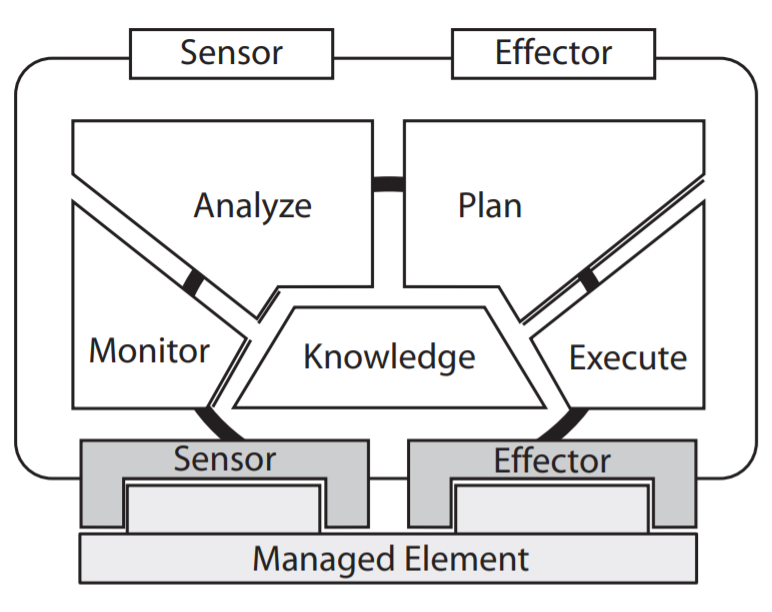
\includegraphics[scale=0.5]{images/MAPE-K.png}
\caption {Diagrama de funcionamento da arquitetura MAPE-K~\citep{Abbas_2010}.}
\label{fig:MAPEK}
\end{figure}

\subsection{Arquitetura \textit{Pipes-and-Filters}}

Em uma arquitetura \textit{Pipes-and-Filters}, ilustrada na Figura \ref{fig:PipeandFilter}, cada componente tem um conjunto de entradas e um conjunto de saídas. Um componente lê \textit{streams} (ou fluxos) de dados em suas entradas e produz \textit{streams} de dados em suas saídas, abstraindo a entrega de um resultado como um todo. O \textit{stream} de entrada é transformado de modo que a saída comece a ser produzida antes da entrada ser completamente consumida. Por isso, os componentes são chamados de filtros (\textit{filters}). Os conectores deste estilo servem como condutores para os \textit{streams}, transmitindo as saídas de um filtro para as entradas de outro. Por isso, os conectores são chamados de tubos (\textit{pipes})~\citep{Garlan_1993}.

\begin{figure}[h]
\centering
\includegraphics[scale=0.25]{images/PipeandFilter.png}
\caption {Diagrama de uma arquitetura \textit{Pipes-and-Filters}.}
\label{fig:PipeandFilter}
\end{figure}

Os filtros devem ser independentes, isto é, não devem compartilhar estado com outros filtros e, durante a programação, o ideal é que os filtros independam da ordem de processamento. Suas especificações podem restringir os dados transportados nos \textit{pipes} de entrada e nos \textit{pipes} de saída, mas não conhecem quaisquer outros filtros, ou componentes, conectados por seus \textit{pipes}. Especializações comuns desse estilo incluem \textit{pipelines}, que restringem as topologias a sequências lineares de filtros; \textit{Pipes} limitados, que restringem a quantidade de dados que podem ser passados em um \textit{pipe}, e \textit{pipes} tipados, que exigem que os dados passados entre dois filtros tenham um tipo bem definido.

O uso da arquitetura \textit{Pipes-and-Filters} possui como vantagens:

\begin{itemize}
\item Permite que o Arquiteto de Software/Desenvolvedor entendam o comportamento geral de entrada/saída de um sistema como uma composição simples dos comportamentos dos filtros individuais.
\item Suporta a reutilização: quaisquer dois filtros podem ser conectados, desde que concordem com os dados que estão sendo transmitidos entre eles. 
\item Os sistemas podem ser facilmente mantidos e aprimorados: novos filtros podem ser adicionados a sistemas existentes e filtros antigos podem ser substituídos por outros melhorados.
\item Permitem certos tipos de análise especializada, como análise de rendimento e de impasse.
\item Naturalmente suportam a execução simultânea: Cada filtro pode ser implementado como uma tarefa separada e potencialmente executado em paralelo com outros filtros.
\end{itemize}

Como desvantagens, é possível citar:

\begin{itemize}
\item Geralmente levam a uma organização de processamento em lote. Embora os filtros possam processar dados de forma incremental, uma vez que os filtros são inerentemente independentes, o Arquiteto de Software é forçado a pensar em cada filtro como fornecendo uma transformação completa dos dados de entrada em dados de saída. 
\item Por sua natureza de transformação de dados, os sistemas que usam a arquitetura \textit{Pipes-and-Filters} normalmente não são bons para lidar com aplicativos interativos. Esse problema é mais grave quando são necessárias atualizações de exibição incrementais, porque o padrão de saída para atualizações incrementais é radicalmente diferente do padrão para saída de filtro.
\item Podem ser prejudicados por terem que manter correspondências entre dois \textit{streams} separados, mas relacionados. 
\item Podem forçar um resultado médio na transmissão de dados em situações onde muitos filtros sejam encadeados com um único filtro, resultando em trabalho adicional para cada filtro separar seus dados e analisar o que for necessário. Isso, por sua vez, pode levar tanto à perda de desempenho quanto ao aumento da complexidade na escrita dos próprios filtros.
\end{itemize}

\section{Ciência de Dados e Engenharia de Dados}

\subsection{Engenharia de Dados}

A engenharia de dados é o meio para entender um processo. Os dados podem ser gerados de várias maneiras, ou um subconjunto dos dados disponíveis pode usar técnicas de análise de dados de estatísticas, aprendizado de máquina, reconhecimento de padrões ou redes neurais, juntamente com outras tecnologias, como visualização, otimização, sistemas de banco de dados. dados, ferramentas de prototipagem e elicitação de conhecimento. O objetivo é usar os dados disponíveis ou gerar mais dados e assim entender o processo que está sendo investigado. O processo de analisar os dados, criar novas ferramentas de análise especificamente para a tarefa e trabalhar com especialistas do domínio é um aspecto fundamental dessa tarefa de engenharia. Atualmente é muito utilizado em conjunto com o termo \textit{Big Data}, para a limpeza, tratamento e estabelecimento de processos para governança de grandes volumes de dados.

O termo \textit{Big Data} apareceu uma vez como conceito em 1974 e novamente em editoriais em 2006 e 2007, e somente em 2008 seu uso como conceito começou a aparecer regularmente em artigos científicos, mas implementações desse conceito começaram a partir de 2010~\citep{Raban_2020}. Quanto a engenharia de dados, embora periódicos como o IEEE Transactions on Knowledge and Data Engineering, cuja primeira edição foi lançada em 1989, e conferências como a IEEE International Conference on Data Engineering (ICDE), cuja primeira edição foi realizada em 1984, possam ser consideradas pontapés iniciais para discussões e artigos acadêmicos, o embrião da engenharia de dados vem do \textit{paper} \textit{"A Business Intelligence System"}, de 1958~\citep{Panoply_2017}. Nele, é mencionada a ideia de sistemas rodados por máquinas para abstrair e padronizar informações de vários setores da sociedade, como industrial, científico e de organizações governamentais, e como estas podem disseminar informação de uma maneira mais eficiente. Embora os anos 50/60 foram o embrião para o conceito, os anos 70/80 o amadureceram e construíram a base para a estrutura de engenharia de dados~\citep{Panoply_2017}.

Nos anos 70/80, os problemas em engenharia de dados eram classificados de acordo com 3 atributos~\citep{IEEE_1989}:

\begin{itemize}
\item \textbf{Completude do conhecimento e dos dados:} Os dados e o conhecimento disponíveis no ambiente poderiam ser considerados como \textit{completos} ou \textit{incompletos}. Se estiverem \textit{completos}, não seria necessário congecimento adicional para a resolução do problema. Se estiverem \textit{incompletos}, como no caso de grandes volumes de dados onde é exigida uma sumarização mais detalhada, seria necessário determinar heurísticas para encontrar um conjunto de dados mais específico para a resolução do problema.
\item \textbf{Exatidão do conhecimento e dos dados:} Os dados e o conhecimento disponíveis no ambiente poderiam ser considerados como exatos ou inexatos. Se estiverem exatos, poderiam ser representados em uma forma numérica ou lógica, como datas e coordenadas. Se estiverem inexatos, o número de casos possíveis seria infinito e seria impossível enumerar ou representar todos eles, sendo necessário determinar heurísticas para definir um número finito de possibilidades ou redefinir o significado de exatidão para que o que está disponível possa ser tratado como exato, como o reconhecimento de um objeto em uma imagem ou a definição do menor custo em uma determinada rota.
\item \textbf{Conhecimento sobre o objetivo e especificações do problema:} Um objetivo de um problema pode ser bem ou mal definido. Um objetivo bem definido podia ser medido e representado em termos de parâmetros para que seja possível comparar a qualidade de uma solução com outra, enquanto um objetivo mal definido envolvia parâmetros que não podem ser mensurados ou não poder ser medido, sendo impossível comparar a qualidade de soluções alternativas e necessitando de tratamentos adicionais para que o objetivo deixe de ser mal definido e passe a ser bem definido. 
\end{itemize}

Dado estas categorias, é possível pensar em soluções que conversam com os objetivos da Engenharia de Software: Abordar diversos tipos de conceitos; como teoria, projeto, desenvolvimento, avaliação e manutenção de novos dados e técnicas, metodologias e sistemas de gerenciamento de conhecimento; em prol do desenvolvimento e manutenção de sistemas e soluções com qualidade e com o custo mais viável possível. Estes sistemas podem ter questões relacionadas ao cumprimento desses objetivos incluindo estudos sobre os aspectos teóricos, ferramentas e metodologias de projeto, tradeoffs de projeto, representação e programabilidade, algoritmos e controle, confiabilidade e tolerância a falhas e projetos usando tecnologias existentes e emergentes. É tarefa do engenheiro de dados elaborar processos que reflitam tais questões em um sistema com objetivos definidos.

\subsection{Ciência de Dados}

Ciência de dados como um conceito precedeu o \textit{Big Data}, sendo um conjunto de princípios fundamentais que apoiam e orientam a extração baseada em princípios de informação e conhecimento de dados~\citep{Raban_2020}. Essa definição enfatiza a estreita relação de ciência de dados com a mineração de dados e, consequentemente, com a engenharia de dados. O termo foi cunhado nos anos 60 para descrever uma nova profissão que daria suporte à compreensão e interpretação da grande quantidade de dados que estavam sendo acumulados na época~\citep{Foote_2021}. Na academia, o termo começou a ser utilizado de modo mais formal a partir de 2001, quando os títulos dos artigos científicos começaram a usar, embora artigos já estavam focando em ciência de dados e usando o termo desde os anos 60~\citep{Raban_2020}~\citep{Foote_2021}. 

A estatística e o uso de modelos estatísticos estão profundamente enraizados no campo da ciência de dados, pois começou com estatísticas e evoluiu para incluir conceitos e práticas principalmente para aplicações de IA. À medida que mais e mais dados se tornam disponíveis, por meio de comportamentos e tendências registradas em softwares espalhados pela Internet ou mesmo por aplicações empresariais, as empresas os coletam e armazenam em quantidades cada vez maiores. Uma vez que as portas foram abertas por empresas que buscam aumentar os lucros e impulsionar melhores tomadas de decisão, seu uso, em conjunto com \textit{Big Data}, começou a ser aplicado a outros campos, como medicina, engenharia e ciências sociais.

Um cientista de dados funcional, ao contrário de um estatístico geral, tem compreensão da arquitetura de software e entende várias linguagens de programação. O cientista de dados define o problema, identifica as principais fontes de informação e projeta a estrutura para coletar e rastrear os dados necessários. O software é normalmente responsável por coletar, processar e modelar os dados. Eles usam os princípios da ciência de dados e toda sua visão multidisciplinar para obter conhecimentos mais profundos. A ciência de dados continua a evoluir como uma disciplina que usa ciência da computação e metodologia estatística para fazer previsões úteis e obter insights em uma ampla gama de campos. Embora seja usada em áreas como astronomia e medicina, também é usada nos negócios para ajudar a tomar decisões mais inteligentes.

\subsection{O ciclo do dado: Semelhanças e diferenças entre Engenharia de Dados}

Nos tempos atuais, empresas e instituições acadêmicas utilizam Engenharia de Dados e Ciência de Dados para otimizar as suas aplicações de IA. Embora tais termos sejam distintos e seus profissionais performem tarefas distintas, na prática é frequente a função de engenharia de dados ser feita por cientistas de dados e vice-versa pois ambas se complementam muito na criação de aplicações de IA. Um bom exemplo de como estas áreas se conversam está no \textit{paper} \textit{Concise Survey of Computer Methods}, de 1974~\citep{Panoply_2017}. Nele, Peter Naur detalha diversos métodos de processamento de dados e aplicações, o que poderia definir como um, mas a citação mais importante de seu \textit{paper} está justamente no termo ciência de dados. Também define que a utilidade de um dado e de seus processos deriva de sua aplicação no desenvolvimento e manutenção de modelos da realidade~\citep{Foote_2021}. Em outras palavras, a existência de um processo que trate os dados é tão importante quanto a construção de um modelo através de seus dados. Ao entender como os dados devem ser usados, é possível criar processos que auxiliem a otimizar os resultados obtidos e criar modelos cada vez mais próximos da realidade.

A principal razão para ambas as áreas se conversarem esta no ciclo de vida do dado, fundamental para entender as oportunidades e os desafios de aproveitar ao máximo os dados digitais. Como um ser vivo, os dados têm um ciclo de vida, desde o nascimento, passando por uma vida ativa até alguma forma de expiração, podendo ser "imortalizado" dependendo de sua importância. Também como um organismo vivo e inteligente, sobrevive em um ambiente que fornece suporte físico, contexto social e significado existencial~\citep{Berman_2018}.

\begin{figure}[h]
\centering
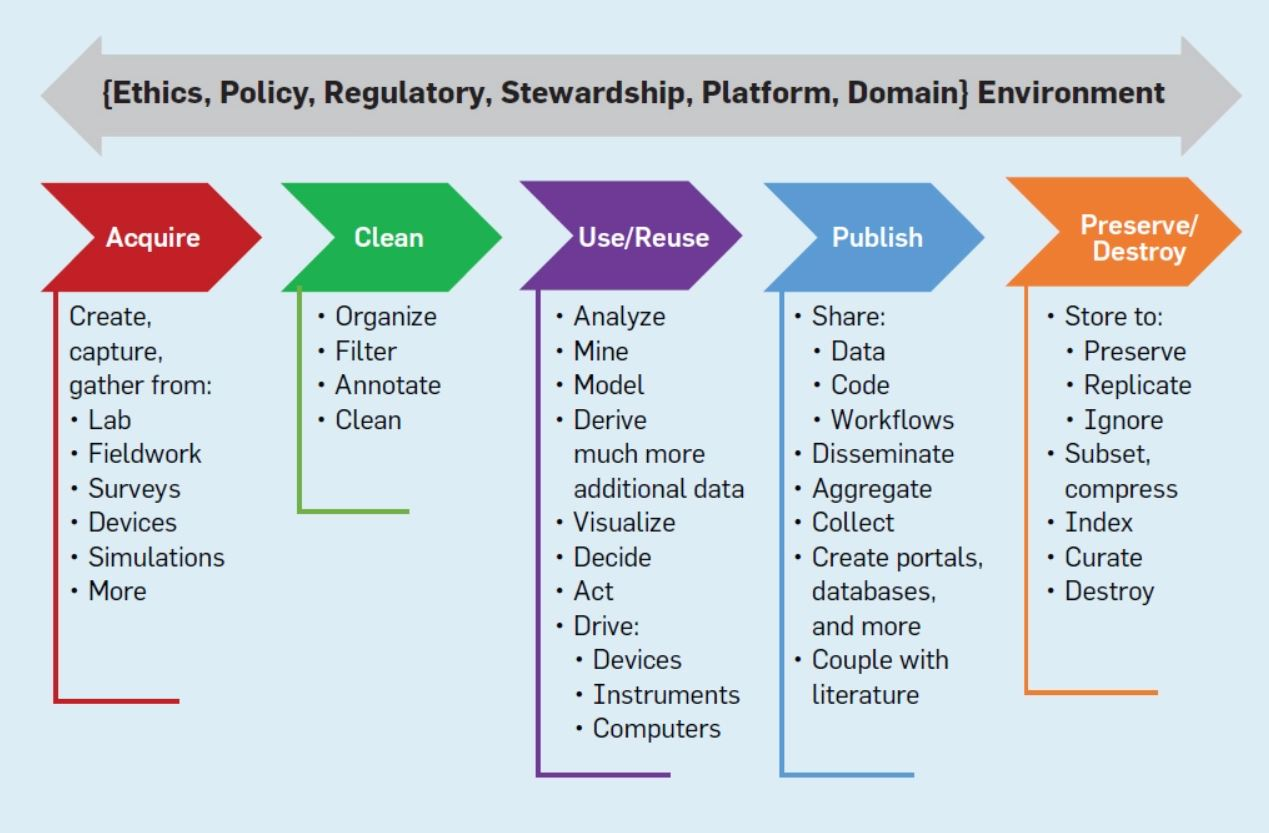
\includegraphics[scale=0.6]{images/data_life_cycle.jpg}
\caption {Ciclo de vida e ecossistema do dado~\citep{Berman_2018}.}
\label{fig:cicloDado}
\end{figure}

Este ciclo, ilustrado na Figura \ref{fig:cicloDado}, é dividido em 5 etapas:

\begin{itemize}
\item \textbf{Aquisição:} Refere-se a processos de criação e coleta de dados, através de experimentos, sensores, pesquisas, sistemas, simulações, entre outros processos
\item \textbf{Limpeza:} Refere-se a processos de limpeza, organização e filtragem dos dados adquiridos.
\item \textbf{Uso/Reuso:} Refere-se a aplicações que os dados podem ter para a aquisição de novos conhecimentos, como análise, mineração, modelagem, enriquecimento, sintetização de novos dados, visualização e tomadas de decisão.
\item \textbf{Publicação:} Refere-se ao compartilhamento destes dados após seu uso, podendo ter como meio alguma plataforma de compartilhamento, bases de dados ou artigos acadêmicos.
\item \textbf{Preservação/Destruição:} Refere-se a processos de armazenamento, curadoria e validação do dado após seu uso e publicação. No contexto de validação, se o mesmo ainda continua útil para o contexto em que foi coletado, podendo ser atualizado ou destruído em caso negativo. Também pode ser comprimido ou indexado caso espaço ou desempenho sejam considerados gargalos para os usuários que forem usar os dados publicados.
\end{itemize}

Como exemplo, é possível citar os dados para experimentos do Grande Colisor de Hádrons (LHC), representando colisões de partículas dentro de um túnel de 17 milhas para testar as previsões de várias teorias da física de partículas e da física de alta energia~\citep{Berman_2018}. A maioria dos dados gerados é tecnicamente irrelevante e são descartados, mas isso não impede que uma enorme quantidade de dados seja influente e continue a ser analisada e preservada. Em 2012, dados sobre experimentos do LHC forneceram fortes evidências para o bóson de Higgs, apoiando a veracidade do Modelo Padrão da Física. Esta descoberta científica foi a "Descoberta do Ano" de 2012 da revista Science e o Prêmio Nobel de Física em 2013.

As estimativas são de que, em 2040, haverá de 10 exabytes a 100 exabytes de dados influentes produzidos pelo LHC. Os dados retidos do LHC são anotados, preparados para preservação e arquivados em mais de uma dúzia de locais físicos. O resultado desse processo é divulgado à comunidade para análise e uso em mais de 100 outros locais de pesquisa. Além do desenvolvimento de protocolos de administração, disseminação e uso de dados, o ecossistema de dados do LHC também fornece um modelo econômico que suporta de forma sustentável os dados e sua infraestrutura. Essa combinação entre administração dos dados e administração econômica permitem que os dados sejam mantidos.

O diagrama do ciclo de vida dos dados descrito na figura e o exemplo do LHC sugerem um conjunto contínuo de ações e transformações nos dados, mas em muitas comunidades científicas e disciplinas hoje essas etapas são isoladas. Os cientistas de domínio se concentram em gerar e usar dados. Cientistas da computação podem se concentrar em questões de plataforma e desempenho, incluindo mineração, organização, modelagem e visualização, bem como os mecanismos para extrair significado dos dados por meio de aprendizado de máquina e outras abordagens. Estatísticos podem se concentrar na matemática dos modelos de risco e inferência~\citep{Berman_2018}. Engenheiros de dados podem se concentrar na administração e preservação de dados gerados pelo cientista de domínio e no \textit{backend} do pipeline, seguindo a aquisição, decisões e ações no domínio da publicação, arquivamento e curadoria. Cientistas de dados podem unir o trabalho dos cientistas da computação e dos estatísticos para extrair novos conhecimentos e conhecer tomadas de decisão mais eficientes.


\section{Machine Learning}

Aprendizado de Máquina (\textit{Machine Learning}, em inglês) pode ser definido como “a prática de usar algoritmos para coletar dados, aprender com eles, e então fazer uma determinação ou predição sobre alguma coisa no mundo. Então em vez de implementar as rotinas de software manualmente, com um gama específica de instruções para completar uma tarefa em particular, a máquina é `treinada` usando uma quantidade grande de dados e algoritmos que dão e ela a habilidade de aprender como executar a tarefa”~\citep{Copeland_2016}. Com isso, o computador consegue a habilidade de realizar determinado cálculo ou tarefa sem que necessite de programação adicional ou interferência humana para isso.

O \textit{Machine Learning} é fortemente relacionado com a Estatística, uma vez que seus métodos e parte de seus algoritmos, como regressões, tiveram como base modelos estatísticos e a análise de seus dados. As tarefas de aprendizado podem ser classificadas em três categorias básicas~\citep{MLWikipedia_2021}~\citep{MLSAS_2021}:

\begin{itemize}
\item \textbf{Aprendizado supervisionado}: O treinamento é realizado por meio de exemplos rotulados, como uma entrada na qual a saída desejada é conhecida. Através de métodos como classificação, regressão e \textit{gradient boosting}, o aprendizado supervisionado utiliza padrões para prever os valores de rótulos em dados não-rotulados adicionais. O aprendizado supervisionado é comumente empregado em aplicações nas quais dados históricos preveem eventos futuros prováveis.
\item \textbf{Aprendizado não-supervisionado}: É utilizado em dados que não possuem rótulos históricos. A “resposta certa” não é informada ao sistema, o algoritmo deve descobrir o que está sendo mostrado. O objetivo é explorar os dados e encontrar alguma estrutura dentro deles. Técnicas populares incluem mapas auto-organizáveis, mapeamento por proximidade, agrupamento \textit{k-means} e decomposição em valores singulares. Esses algoritmos também são utilizados para segmentar tópicos de texto, recomendar itens e identificar pontos discrepantes nos dados.
\item \textbf{Aprendizado por reforço}: O algoritmo descobre através de testes do tipo “tentativa e erro” quais ações rendem as maiores recompensas. Este tipo de aprendizado possui três componentes principais: o agente (o aprendiz ou tomador de decisão), o ambiente (tudo com que o agente interage) e ações (o que o agente pode fazer). O objetivo é que o agente escolha ações que maximizem a recompensa esperada em um período de tempo determinado. O agente atingirá o objetivo muito mais rápido se seguir uma boa política, então o foco do aprendizado por reforço é descobrir a melhor política.
\end{itemize}

O termo \textit{Machine Learning} se tornou muito mais evidente com a possibilidade da implementação do \textit{Deep Learning}, que é uma técnica que utiliza Redes Neurais Artificiais para atingir seus resultados. Redes Neurais Artificiais são modelos computacionais inspirados no sistema nervoso do cérebro, onde temos neurônios divididos em camadas e conectados entre si, podendo ser abstraído conforme ilustração na Figura \ref{fig:NeuralNetwork}. Dependendo da tarefa a ser realizada, cada neurônio atribui um peso para os dados que entram e a saída final é determinada pelo total desses pesos~\citep{Copeland_2016}. As redes neurais utilizadas em \textit{Deep Learning} possuem, ao menos, duas camadas de neurônios entre a camada que recebe os dados de entrada e a camada final que faz o tratamento final dos dados de saída.

\begin{figure}[h]
\centering
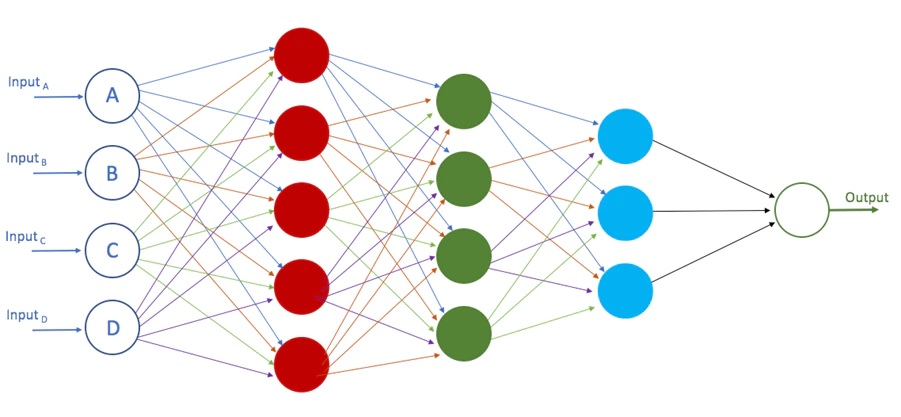
\includegraphics[scale=0.8]{images/deep_neural_network.jpg}
\caption {Exemplo de uma rede neural utilizada em \textit{Deep Learning}.}
\label{fig:NeuralNetwork}
\end{figure}

Com a evolução da computação, o treino de uma tarefa passou a ser cada vez mais viável, uma vez que a execução de algoritmos de \textit{Machine Learning} é computacionalmente muito custosa, especialmente quando redes neurais são utilizadas. Sua viabilidade também se prova quando tais tarefas se tornam efetivas no mundo real: Como exemplo, reconhecimento de imagens por máquinas treinadas através de deep learning em alguns cenários possuem uma taxa de acerto maior que a de humanos~\citep{Copeland_2016}.

\subsection{Métricas de Avaliação}

Tradicionalmente em um problema de classificação binária, uma previsão do classificador pode ter 4 tipos de resultados em uma matriz de confusão, presente na Tabela \ref{tbl:ConfusionMatrix}. Os Verdadeiros Positivos (VP, ou TP pelo termo em inglês \textit{True Positives}) e Verdadeiros Negativos (VN, ou TN pelo termo em inglês \textit{True Negatives}) são classificações corretamente previstas pelo classificador. Um Falso Positivo (FP) ocorre quando um caso previsto para estar na classe positiva quando o resultado real pertence à classe negativa, e um Falso Negativo (FN) ocorre quando um caso previsto para estar na classe negativa
quando o resultado real pertence à classe positiva.

\begin{table}[h]
\label{tbl:ConfusionMatrix}
\begin{center}
  \caption{Matriz de confusão}
  \resizebox{\linewidth}{!}{%
  \begin{tabular}{|c|c|c|c|}
    \hline
    \multicolumn{4}{|c|}{\textbf{Classe prevista}}\\
    \hline
    \multirow{3}{*}[-3ex]{\rotatebox[origin=c]{90}{\textbf{Classe atual}}} &  & \textbf{Positiva} & \textbf{Negativa}\\[3ex]
    \cline{2-4}
     & \textbf{Positiva} & \makecell{Verdadeiros Positivos\\(VP/TP)} & \makecell{Falsos Positivos\\(FP)}\\[3ex]
    \cline{2-4}
     & \textbf{Negativa} & \makecell{Falso Negativo\\(FN)} & \makecell{Verdadeiros Negativos\\(VN/TN)}\\[3ex]
    \hline
  \end{tabular}}
\end{center}
\end{table}

A taxa de sucesso, também conhecida como \textbf{acurácia}, é o número de previsões corretas dividido pelo número total de resultados:

\begin{equation}
Acc = \frac{TP + TN}{TP + TN + FP + FN}
\end{equation}

Ela é considerada um indicador da realização de um bom treinamento e de um bom funcionamento do modelo obtido. Entretanto, não é a melhor métrica para interpretar situações onde a qualidade dos dados utilizados interfere no resultado final, como classes desequilibradas.

A \textbf{precisão} enfatiza situações quando o número de falsos positivos é alto e mostra a precisão das previsões positivas. É a fração de casos positivos previstos corretamente para estar na classe positiva de todos os casos positivos previstos no modelo:

\begin{equation}
P = \frac{TP}{TP + FP}
\end{equation}

O \textbf{recall}, ou sensibilidade, enfatiza situações quando o número de falsos negativos é alto.  É a fração de casos positivos previstos corretamente para estar na classe positiva de todos os casos positivos reais:

\begin{equation}
R = \frac{TP}{TP + FN}
\end{equation}

O \textbf{F1-score} é um caso especial de F-score, uma medida geral da acurácia de um modelo que combina precisão e recall. Pode ser interpretado como uma ponderação entre ambos e usa a média harmônica para realizar a medição:

\begin{equation}
F1 = 2 \times\frac{P \times R}{P + R}
\end{equation}

O \textbf{AUC} (\textit{Area under the ROC Curve}), também chamada de precisão balanceada, pode interpretar a capacidade do classificador de evitar falsos positivos e falsos negativos. Se sai melhor que a acurácia em situações que ela não é apropriada, como o desequilíbrio entre classes já citado anteriormente:

\begin{equation}
AUC = \frac{1}{2} \left( \frac{TP}{TP + FN} + \frac{TN}{TN + FP} \right)
\end{equation}

\subsection{Algoritmos}

Existem diversos algoritmos de \textit{Machine Learning} utilizados para resolver os problemas de aprendizado supervisionado, não-supervisionado e por reforço. Nesta seção serão abordados apenas os algoritmos utilizados por este trabalho de Mestrado.

\subsubsection{Regressão Logística}

A Regressão Logística é um método de classificação baseado na aplicação da técnica de Regressão Linear. Como na Regressão Linear, ele assume uma relação linear entre os recursos e calcula a soma ponderada dos recursos mais um termo de viés. Neste método, o resultado não é utilizado diretamente, mas calcula a logística do resultado. Quando peso das \textit{features} é $w$ e o termo de viés é $b$, a probabilidade estimada do modelo de regressão logística é a seguinte:

\begin{equation}
\hat{p} = \sigma (w^{T}x + b)
\end{equation}

Logo após, a função logística $\sigma$ é calculada:

\begin{equation}
\sigma (z) = \frac{1}{1 + exp(-z)}
\end{equation}

Uma vez que o modelo de Regressão Logística estimou a probabilidade $\hat{p}$, a previsão de classificação é feita considerando a seguinte regra:

\begin{equation}
	\begin{aligned}
	\hat{p} = 
	\begin{cases}
	1 & \text{Se $\hat{p} \geq 0,5$}\\
	0 & \text{Se $\hat{p} < 0,5$}\\
	\end{cases}
	\end{aligned}
\end{equation}

O objetivo do treinamento de um modelo de classificação é de minimizar a diferença entre o resultado atual e o resultado previsto. Para medir o quão próximo a função resultante do treinamento se aproxima do conjunto de dados, a seguinte função de custo é calculada conforme equação abaixo. A função utilizada pode variar, tendo como exemplos a função por entropia cruzada ou a função por diferença de quadrados.

\begin{equation}
J(w,b) = \frac{1}{m} \sum^{m}_{i=1} L(\hat{y}^{(i)}, y^{(i)})
\end{equation}

Durante o treinamento do modelo de Regressão Logística, é preciso encontrar os parâmetros $w$ e $b$ que minimizem a função de custos globais. Como a função de custo é convexa, diferentes métodos de otimização, como o gradiente descendente, garantem encontrar o mínimo global.

Para lidar com problemas com múltiplas classes para classificação, é possível calcular uma função de custo separada para cada rótulo de classe por observação e somar os resultados, técnica conhecida como \textit{One-Vs-All}~\citep{Rifkin_2004}. Outra técnica que pode generalizar o método de regressão logística para suportar várias classes diretamente é chamada de Regressão Softmax, ou Regressão Logística Multinomial, utilizando a função Softmax para substituir a função de probabilidade da Regressão Logística convencional:

\begin{equation}
\hat{p}(Y_i = n) = \frac{e^{\beta_{n} \cdot \textbf{X}_{i}}}{1 + \sum^{K-1}_{k=1} e^{\beta_{k} \cdot \textbf{X}_{i}}}
\end{equation}

\subsubsection{\textit{Support Vector Machines} (SVM)}

\textit{Support Vector Machines} (SVM) é um algoritmo de aprendizado de máquina que pode ser usado para detecção linear, não linear, de classificação, regressão e até mesmo detecção de anomalias (\textit{Outliers}). A ideia fundamental por trás dessa técnica é que as classes de saída são separadas com um hiperplano maximizando a margem (distância máxima entre os pontos de dados de ambas as classes)~\citep{Steinwart_2008}. As \textit{Support Vector Machines} criam um ou vários hiperplanos em um espaço de $n$ dimensões. A dimensão dos hiperplanos depende do número de \textit{features}. Quando há duas \textit{features}, é apenas uma linha, ou quando há três \textit{features}, é um plano bidimensional.

Para lidar com conjuntos de dados não lineares, uma abordagem é adicionar mais \textit{features}, como um recurso polinomial, ou a outra abordagem é usar \textit{kernels}, mapeando os dados de entrada de $n$ dimensões para um espaço de dimensão superior, onde os dados podem ser separados linearmente.

\subsubsection{Regressão Kernel Ridge}

A Regressão Kernel Ridge (\textit{Kernel Ridge Regression}/KRR) é um algoritmo de aprendizado de máquina proveniente da combinação de duas operações: A Regressão Ridge com o que é conhecido como "truque do kernel"~\citep{Witten_2016}. A Regressão Ridge substitui a função de custo tradicional por uma com um termo de penalização incluído, conforme ilustrado na Equação \ref{eqn:kernelLeastSquares}, utilizando o método dos mínimos quadrados. O "truque do kernel" é uma técnica mátemática que permite exemplificar problemas não-lineares de forma linear utilizando kernels, reduzindo a complexidade para uma simples operação matricial.

\begin{equation}
\label{eqn:kernelLeastSquares}
\sum_{i} (y_{i} - w^{T}x_i)^{2} - \lambda \norm{w}^{2}
\end{equation}

Por causa de tais operações, A Regressão Kernel Ridge exige mais processamento do que uma regressão tradicional. No entanto, é vantajoso usá-la em casos que um ajuste não-linear é desejado ou onde há mais atributos do que elementos no conjunto de treinamento. Em casos onde há mais elementos no conjunto de treinamento do que atributos, a Regressão Kernel Ridge peca por não abranger o conceito utilizado nas \textit{Support Vector Machines}, onde é necessário somar apenas o conjunto de vetores de suporte ao invés de todo o conjunto de treinamento. No entanto, por causa deste mesmo conceito as \textit{Support Vector Machines} exigem mais processamento.

\subsubsection{Árvores de Decisão (\textit{Decision Trees})}

Árvores de decisão (\textit{Decision Trees}) são um grupo de algoritmos de aprendizado de máquina que podem ser usados para classificação e regressão. Eles são os métodos de aprendizado mais comuns que são muito poderosos e capazes de ajustar conjuntos de dados complexos. Os algoritmos de Árvore de Decisão são baseados em uma abordagem de dividir e conquistar para os problemas de classificação~\citep{Witten_2016}. Uma Árvore de Decisão é feita pelo processo contínuo de dividir o conjunto de dados nos atributos da melhor maneira possível em diferentes classes até que um critério de parada específico seja alcançado. Nas Árvores de Decisão, as observações sobre os itens são mostradas em ramificações e as conclusões das observações são mostradas nos nós. Existem três tipos diferentes de nós: os nós raiz que indicam o início do processo de decisão e não têm arestas de entrada, os nós internos que têm exatamente uma entrada e pelo menos duas arestas de saída e os nós finais (ou as folhas).

Sempre que o rótulo de classificação de destino assume valores discretos, a Árvore de Decisão é chamada de árvore de classificação e, sempre que recebe valores contínuos, é chamada de árvore de regressão. Um dos méritos do uso de Árvores de Decisão é que elas exigem pouco pré-processamento de dados e não há necessidade de escala. Seu treinamento geralmente é realizado com uma árvore menos complicada e mais abrangente. A complexidade de uma Árvore de Decisão pode ser controlada usando critérios de parada e métodos de poda~\citep{Rokach_2005}, existindo quatro métricas diferentes para poder medí-la: o número total de nós, o número total de folhas, a profundidade da árvore e o número de atributos usados.

Os algoritmos usados para construir uma Árvore de Decisão a partir de um conjunto de dados são chamados de indutores. Normalmente, o objetivo desses algoritmos é encontrar a Árvore de Decisão ótima minimizando o erro de generalização, considerando o número mínimo de nós e a profundidade mínima da árvore. Os algoritmos da Árvore de Decisão funcionam de forma \textit{top-down}, pois escolhem a melhor variável em cada estágio que pode dividir o conjunto de dados em um atributo específico. Diferentes indutores usam critérios diferentes para encontrar a melhor variável.

\subsubsection{\textit{Random Forest}}

\textit{Random Forest} é um algoritmo de aprendizado de máquina que combina a simplicidade das Árvores de Decisão com a flexibilidade, resultando em melhorias na acurácia~\citep{Breiman_2001}. Neste algoritmo, o \textit{Bagging}, uma técnica que gera uma coleção de classificadores introduzindo subconjuntos randômicos na entrada do algoritmo~\citep{Witten_2016}, é utilizado para gerar uma coleção de Árvores de Decisão simplificadas com a finalidade de generalizar o resultado no conjunto da obra.

No final, a classe selecionada é a que for mais citada dentre essa coleção. Esta simplificação, em geral, otimiza o treinamento em relação a uma Árvore de Decisão tradicional.

\subsubsection{\textit{Gradient Boosting}}

\textit{Gradient Boosting}, também conhecido como \textit{Gradient Boosting Machine} (GBM) ou \textit{Gradient Boosted Regression Tree} (GBRT)~\citep{Chen_2016}, é um algoritmo de aprendizado de máquina que faz a classificação através da composição de pequenos modelos pela utilização do \textit{Boosting}~\citep{Friedman_2000}~\citep{Hastie_2009}. \textit{Gradient Boosting} faz uso de \textit{Boosting} para gradualmente aproximar um melhor modelo, de modo a somar submodelos ao modelo composto. Árvores de Decisão tendem a gerar \textit{overfitting}, e o \textit{Gradient Boosting} é uma possibilidade para solucionar este problema.

\textit{Boosting} é uma combinação de modelos simples, chamados de modelos fracos, onde tipicamente estes modelos são Árvores de Decisão. O algoritmo combina classificadores fracos com intuito de produzir um classificador forte. Diferente do \textit{Bagging}, a obtenção de subconjuntos vindos do conjunto de dados não é feita de maneira aleatória, e sim feita priorizando a substituição de dados mal classificados, que ganham um peso maior para serem substituídos nas iterações seguintes~\citep{Hastie_2009}.

\subsubsection{Redes Neurais Artificiais}

As Redes Neurais Artificiais, muitas vezes chamadas apenas de Redes Neurais, são um grupo de métodos de modelagem de dados estatísticos não lineares, que a princípio foram inspirados nos cérebros e nas estruturas dos neurônios biológicos. Elas são a base do aprendizado profundo, sendo escaláveis e capazes de trabalhar com grandes tarefas complexas de aprendizado de máquina, como serviços de reconhecimento de imagem e reconhecimento de fala. O processo simplificado para treinamento de uma Rede Neural é o seguinte:

\begin{enumerate}[label=\textbf{\arabic*.}]
\item Os dados de entrada são fornecidos à rede, eles se propagam pelas camadas e o processo de encaminhamento produz a previsão.
\item Calcula-se o erro entre o produto previsto e o produto real (função de custo).
\item A Rede Neural usa um algoritmo de otimização para ajustar os pesos de forma a reduzir a função custo.
\item O processo de encaminhamento inicia novamente e continua até que a taxa de erro seja minimizada a um determinado valor, ou até um certo número de iterações.
\end{enumerate}

As Redes Neurais Artificiais não são novas para os sistemas de computação, pois foram introduzidas pela primeira vez por Warren McCulloch e Walter Pitts em 1943~\citep{McCulloch_1943}. Desde então, o desenvolvimento dessas técnicas passou por altos e baixos até ter uma adoção considerável graças aos avanços significativos tanto no poder computacional dos hardwares quanto nas otimizações de algoritmos implementadas nos softwares. Atualmente, é possível treinar Redes Neurais de grande complexidade, e há uma enorme quantidade de dados disponíveis para uso em bancos de dados. Elas podem ser divididas em dois grupos principais~\citep{Singh_2009}:

\begin{itemize}
\item \textbf{Redes retroalimentadas (\textit{Feedforward})}: Nessas redes, o fluxo de dados se move apenas na direção direta da camada de entrada para os nós de saída. Não há alimentação ou loop no sistema.
\item \textbf{Redes recorrentes}: Este tipo de rede pode ter a opção de feedback e reutiliza os dados dos estágios posteriores para os estágios anteriores.
\end{itemize}

Algoritmos de otimização são métodos usados para minimizar o valor da função de custo ajustando os parâmetros internos do modelo. Algumas das técnicas de otimização mais comuns nas estruturas de aprendizado profundo são as seguintes: \textit{Stochastic Gradient Descent} (SGD)~\citep{Schmidt_2013}, \textit{Momentum}~\citep{Polyak_1964}, \textit{Nesterov Accelerated Gradient} (NAG)~\citep{Sutskever_2013}, \textit{Adaptive Gradient} (AdaGrad)~\citep{Duchi_2011}, \textit{Root mean square prop} (RMSprop)~\citep{Graves_2013}, \textit{Adaptive moment estimation}, (Adam)~\citep{Kingma_2014}, \textit{Nesterov and Adam optimizer} (Nadam)~\citep{Dozat_2016}.

Toda Rede Neural consiste em alguns nós (neurônios), conexões ponderadas entre os nós e uma abordagem computacional chamada função de ativação usada para definir a saída de cada neurônio. Diferentes tipos de funções de ativação podem ser usados com esta técnica, como sigmóide, tanh (tangente hiperbólica) ou ReLU (sigla de \textit{Rectified Linear Unit}).

Redes Neurais consistem em diferentes camadas. O tipo mais simples de Rede Neural inclui uma camada de entrada que recebe informações de fontes externas, como valores de atributos do conjunto de dados de entrada. A camada de saída gera a saída da rede e as camadas ocultas conectam a camada de entrada e a camada de saída entre si. O valor de entrada de cada nó em cada camada é calculado pela soma de todos os nós de entrada multiplicada pelo respectivo peso da interconexão entre os nós~\citep{Erb_1993}.

\section{Fairness em Machine Learning}

Como a coleta de dados está presente atualmente no dia-a-dia de variados setores da sociedade, o uso de \textit{Machine Learning} é extremamente versátil para tomadas de decisão, podendo ser utilizados em problemas como admissão de universidades, contratações, análise de crédito e reconhecimento de doenças. Com o aumento dessa influência, o uso de dados sensíveis em um contexto determinado também aumentou, e temas como uma IA ética e conceitos como vieses nos dados e \textit{Fairness} passaram a serem discutidas não apenas na Computação, mas em áreas como Direito. Algoritmos são mais objetivos, rápidos e são capazes de considerar uma grande magnitude de recursos que pessoas não são capazes. Entretanto, até o presente momento eles não são capazes de diferenciar contextos sociais, onde um resultado mais eficiente de acordo com os dados disponíveis podem amplificar as desigualdades sociais e tomar decisões de modo injusto~\citep{Mehrabi_2021}. 

Estes dados sensíveis, tendo como exemplos cor de pele, raça, sexo, idade e altura, são considerados atributos protegidos, que precisam ser classificados e processados antes da execução de um algoritmo de \textit{Machine Learning}, determinarão como o algoritmo se comportará e, consequentemente, afetará suas métricas~\citep{Mougan_2022}. Os grupos de dados provenientes destes atributos protegidos são considerados grupos protegidos, que podem ser divididos em dois grupos: o grupo privilegiado, que possui vantagens no contexto do problema, e o grupo não-privilegiado, que possui desvantagens no contexto do problema e, portanto, sujeito a discriminação.

É possível descrever o conceito de \textit{Fairness} no contexto de aprendizagem supervisionada, onde um modelo $f$ pode prever um conjunto de resultados $y$ a partir de um conjunto de \textit{features} $x$, evitando discriminação injusta em relação a um atributo protegido $a$. É permitido, mas não exigido, que $a$ seja um componente de $x$~\citep{Begley_2021}. Em outras palavras, um modelo de ML considerado justo é aquele onde a correlação de seu resultado é baixa em relação a dados de entrada considerados como sensíveis a discriminações.

Geralmente, as descrições de justiça se dividem em dois grupos principais: justiça individual e justiça de grupo. O objetivo da justiça individual é que indivíduos semelhantes devem obter resultados semelhantes, enquanto na justiça de grupo, cada um dos grupos definidos pelo atributo protegido devem ser tratados igualmente. No geral, os estudos atuais costumam realizar seus experimentos em casos de justiça de grupo, uma vez que o escopo de justiça de grupo é muito mais amplo e tende a exemplificar melhor a relação entre dados, relações sociais e vieses do mundo atual.

\subsection{Métricas de Fairness}

Para avaliar a justiça de um modelo, as métricas utilizadas diferem das métricas utilizadas para avaliação do modelo, que possuem o propósito de verificar se um modelo tem previsões confiáveis ou não. As métricas de \textit{Fairness} possuem um propósito diferente, pois verificam os dados de forma mais intimista. Elas não medem o modelo como um todo, mas o quanto os grupos e registros avaliados estão próximos dos outros. Enquanto as métricas mais tradicionais avaliam a performance do modelo e seus dados como um todo e seus resultados gerais, as métricas de \textit{Fairness} avaliam se os resultados gerais também se refletem em grupos específicos, para verificar se não há disparidade ou discriminação nos resultados propostos.

Assim como algumas métricas utilizadas para avaliação, muitas métricas utilizam Verdadeiros Positivos, Verdadeiros Negativos, Falsos positivos e Falsos Negativos para analisar o quão justo o modelo é. Entretanto, diferente da acurácia, precisão e recall utilizados anteriormente, a medição das discriminações utiliza outras métricas, utilizadas ou não para avaliar a performance, para estabelecer novas métricas mais adequadas para a sua finalidade.

Exemplos de métricas utilizadas para isso são a Taxa de Verdadeiros Positivos e a Taxa de Falsos Positivos. Enquanto a \textbf{Taxa de Verdadeiros Positivos} (ou TPR, pelo termo em inglês \textbf{True Positive Rate}) é outro termo para denominar o recall, a \textbf{Taxa de Falsos Positivos} (ou FPR, pelo termo em inglês \textbf{False Positive Rate}) é a fração de casos negativos previstos incorretamente como estando na classe positiva de todos os casos positivos reais:

\begin{equation}
FPR = \frac{FP}{FP + TN}
\end{equation}

Dada essas métricas iniciais, considerando $Y=1$ a classe positiva, $Z=0$ o grupo não-privilegiado e $Z=1$ o grupo privilegiado, algumas das definições de \textit{Fairness} mais usadas são as seguintes:

\begin{itemize}
\item \textbf{Diferença de paridade estatística (\textit{Statistical parity difference}), ou discriminação~\citep{Zemel_2013}:} Esta métrica é baseada na seguinte fórmula:

\begin{equation}
Pr(Y=1|Z=0)-Pr(Y=1|Z=1)
\end{equation}
 
Aqui, o viés ou paridade estatística é a diferença entre a probabilidade de que um indivíduo aleatório retirado dos não-privilegiados seja rotulado como 1 e a probabilidade de que um indivíduo aleatório dos privilegiados seja rotulado como 1. Portanto, um valor próximo de 0 é considerado justo.

\item \textbf{Diferença de oportunidade igual (\textit{Equal opportunity difference})~\citep{Biswas_2020}:} É a diferença entre a taxa positiva verdadeira do grupo não privilegiado e a taxa positiva verdadeira do grupo privilegiado:

\begin{equation}
TPR_{Z=0} - TPR_{Z=1}
\end{equation}
 
Um valor próximo de 0 é considerado justo. Um classificador binário satisfaz a igualdade de oportunidades quando a taxa positiva verdadeira de ambos os grupos são iguais~\citep{Hardt_2016}

\item \textbf{Diferença de probabilidade média (\textit{Average odds difference})~\citep{Biswas_2020}:} Essa métrica usa a taxa de falsos positivos e a taxa positiva verdadeira para calcular a tendência, calculando a igualdade de probabilidades com a fórmula:

\begin{equation}
\frac{1}{2}(|FPR_{Z=0} - FPR_{Z=1}|+|TPR_{Z=0} - TPR_{Z=1}|)
\end{equation}
 
Precisa ser próximo a 0 para ser considerado justo.

\item \textbf{Impacto de disparidade (\textit{Disparate impact})~\citep{Biswas_2020}:} Para esta métrica, é usada a seguinte fórmula:

\begin{align*}
\frac{Pr(Y=1|Z=0)}{Pr(Y=1|Z=1)}
\end{align*}

Usa as mesmas probabilidades da diferença de paridade estatística, mas como é calculada como uma proporção o valor esta métrica possui um comportamento não-linear. Desta forma, um valor próximo de 1 é considerado justo.

\item \textbf{Índice de Theil (\textit{Theil index})~\citep{Speicher_2018}:} Esta medida também é conhecida como índice de entropia generalizado, mas com o valor de $\alpha$ usado neste índice igual a 1~\citep{Speicher_2018}. É calculado com a seguinte fórmula:

\begin{align*}
\frac{1}{n}\sum^{n}_{i=0}\frac{b_i}{\mu}\ln{\frac{b_i}{\mu}}
\end{align*}

Onde n é a quantidade de elementos e $b_i$ é obtido com a fórmula $b_i = \hat{y}_i - y_i + 1$. Nesta fórmula, $y_i$ é o conjunto de saídas, $\hat{y}_i$ é o conjunto de previsões dadas pelo modelo. Também precisa ser próximo a 0 para ser considerado justo.

\end{itemize}

\subsection{Algoritmos para redução de vieses}
\label{sec:unbiasedAlgorithms}

Há diversos tipos de algoritmos diferentes na inteligência artificial para redução de vieses, a fim de garantir \textit{Fairness} nos projetos de Aprendizado de Máquina. É possível classificá-los em três categorias diferentes: Algoritmos de pré-processamento, de processamento e de pós-processamento.

Os algoritmos de \textbf{pré-processamento} tentam eliminar a discriminação transformando os dados, antes de executar o algoritmo de treinamento. Tais algoritmos podem ser usados caso seja permitida a modificação dos dados de treinamento~\citep{dAlessandro_2017}, e a ideia por trás de tais algoritmos é que suas previsões serão mais balanceadas se o classificador for treinado com os dados já balanceados~\citep{Kamiran_2009}. Nesta categoria se enquadram os seguintes algoritmos:

\begin{itemize}
\item \textbf{Reposição (\textit{Reweighing})~\citep{Kamiran_2011}:} Pondera os exemplos em cada combinação de grupo e rótulo de maneira diferente para garantir a justiça antes da classificação.

\item \textbf{Removedor de impacto de disparidade (\textit{Disparate impact remover})~\citep{Feldman_2015}:} Edita valores de \textit{features} aumentando a justiça de cada grupo enquanto preserva a ordem de classificação dentro dos mesmos.

\item \textbf{Aprendizado de representações justas (LFR, ou \textit{Learning fair representations})~\citep{Zemel_2013}:} Encontra uma representação latente que codifica os dados, mas ofusca informações dos atributos protegidos.

\item \textbf{Pré-processamento otimizado (\textit{Optimized pre-processing})~\citep{Calmon_2017}:} Aprende uma transformação probabilística que edita \textit{features} e rótulos nos dados efetuando justiça em cada grupo, distorção individual, garantindo a fidelidade de dados através de restrições.
\end{itemize}

Os algoritmos de \textbf{processamento} tentam realizar modificações nos algoritmos de treinamento para mitigar a discriminação durante o processo de treinamento do modelo. Se for permitido fazer mudanças no processo de treinamento, então os algoritmos podem ser usados incorporando mudanças na função de custo ou impondo restrições~\citep{Mehrabi_2021}. Nesta categoria se enquadram os seguintes algoritmos:

\begin{itemize}
\item \textbf{Remoção de viés adversário (Adversarial debiasing)~\citep{Zhang_2018}:} Aprende um classificador que maximiza a precisão e reduz a capacidade de um adversário de depender do atributo protegido nas previsões. Essa abordagem leva a um classificador justo, pois as previsões realizadas pelo classificador não possuem nenhuma informação de discriminação nos grupos.

\item \textbf{Removedor de preconceito (Prejudice remover)~\citep{Feldman_2015}:} Técnica que adiciona no algoritmo escolhido um termo de regularização baseado na discriminação.

\item \textbf{Meta-Algoritmo para classificações justas (Meta-Algorithm for Fair Classification)~\citep{Celis_2019}:} Aprende um classificador compatível com uma gama grande de métricas de Fairness, sendo prático o suficiente para abrangê-las sem grande perda de performance.

\item \textbf{Justiça por Subgrupos Ricos (Rich Subgroup Fairness)~\citep{Kearns_2018}:} Aprende um classificador que procura equalizar as taxas de falsos positivos e falsos negativos entre os dados que envolvem atributos protegidos, considerados como subgrupos.

\item \textbf{Redução por Gradiente Exponencial (Exponentiated Gradient Reduction)~\citep{Agarwal_2018}:} Aprende um classificador baseado em Gradiente Exponencial que tende a minimizar o erro de uma classificação ponderada.

\item \textbf{Redução por busca em grid (Grid Search Reduction)~\citep{Agarwal_2018}~\citep{Agarwal_2019}:} Aprende um classificador baseado na busca em um grid de valores que tende a minimizar o erro de uma classificação ponderada. É mais simples e impreciso que a Redução por Gradiente Exponencial, mas sua escolha pode ser razoável se a quantidade de métricas de Fairness a serem consideradas for pequena.

\end{itemize}

Os algoritmos de \textbf{pós-processamento} utilizam um conjunto de validação, que não foi envolvido no processo de treinamento para melhorar a imparcialidade das previsões~\citep{dAlessandro_2017}. Quando não há possibilidade de fazer alterações nos dados de treinamento ou no treinamento do modelo, apenas algoritmos de pós-processamento podem ser usados. Nesta categoria se enquadram os seguintes algoritmos:

\begin{itemize}
\item \textbf{Igualdade de probabilidade calibrada (Calibrated Equalized odds)~\citep{Pleiss_2017}:} Otimiza as previsões do classificador obtido, calibrando para alterar os rótulos de saída e obter probabilidades igualadas entre os grupos.

\item \textbf{Igualdade de probabilidade (Equalized odds)~\citep{Hardt_2016}:} Resolve um problema linear para alterar os rótulos de saída e obter probabilidades igualadas entre os grupos.

\item \textbf{Classificação baseada em Rejeição de Opções (Reject Option-based Classification)~\citep{Kamiran_2012}:} Dá resultados favoráveis para grupos não privilegiados e resultados desfavoráveis para grupos privilegiados de acordo com uma faixa de confiança.

\end{itemize}

\section{Engenharia de Software}

\subsection{Engenharia de Software para Aplicações de IA}

Quando se fala de Arquitetura e Engenharia de Software, se fala da definição dos componentes de software, suas propriedades externas, e seus relacionamentos com outros softwares para fazer com que um sistema seja documentável, reusável e testável. A preocupação está em como um sistema deve ser organizado e com a estrutura geral desse sistema. Dado as definições sobre IA já detalhadas, é possível encaixar Machine Learning na forma de um processo bem definido, de forma que é possível sistematizar todo esse processo na forma de componentes e definir formas em que o modelo resultante do mesmo é disponibilizado para aplicações externas.

No processo, ilustrado na Figura \ref{fig:MLProcess}, o conjunto de dados passa por um pré-processamento e dividido em dois conjuntos, um para treinamento e outro para teste. O conjunto de treino é utilizado para o algoritmo realizar o processo de treinamento, obtendo um modelo após o término desse processo. O conjunto de testes é utilizado para mensurar se o modelo obtido no processo de treinamento realiza previsões confiáveis ou não.

\begin{figure}[h]
\centering
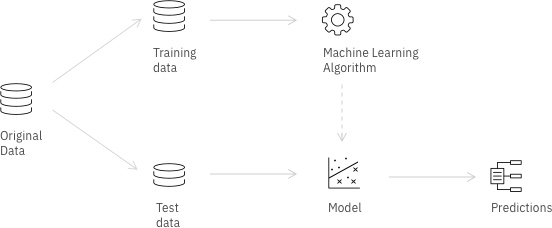
\includegraphics[scale=0.5]{images/ML_Process.jpg}
\caption {Processo padrão para aprendizado de máquina}
\label{fig:MLProcess}
\end{figure}

Um exemplo de arquitetura que generaliza todo o processo, desde a necessidade de negócio até o deploy do modelo de IA, é a IBM Analytics and AI Reference Architecture \citep{IBM_2021}, ilustrada na Figura \ref{fig:AIReferenceArchitecture}. Nela, são definidos os seguintes requisitos não-funcionais: performance, estabilidade, segurança, escalabilidade, manutenibilidade e regulamentações de privacidade/\textit{compliance}, e pode ser classificada em 4 grupos principais envolvendo diversos tipos de processos e componentes:

\begin{figure}[h]
\centering
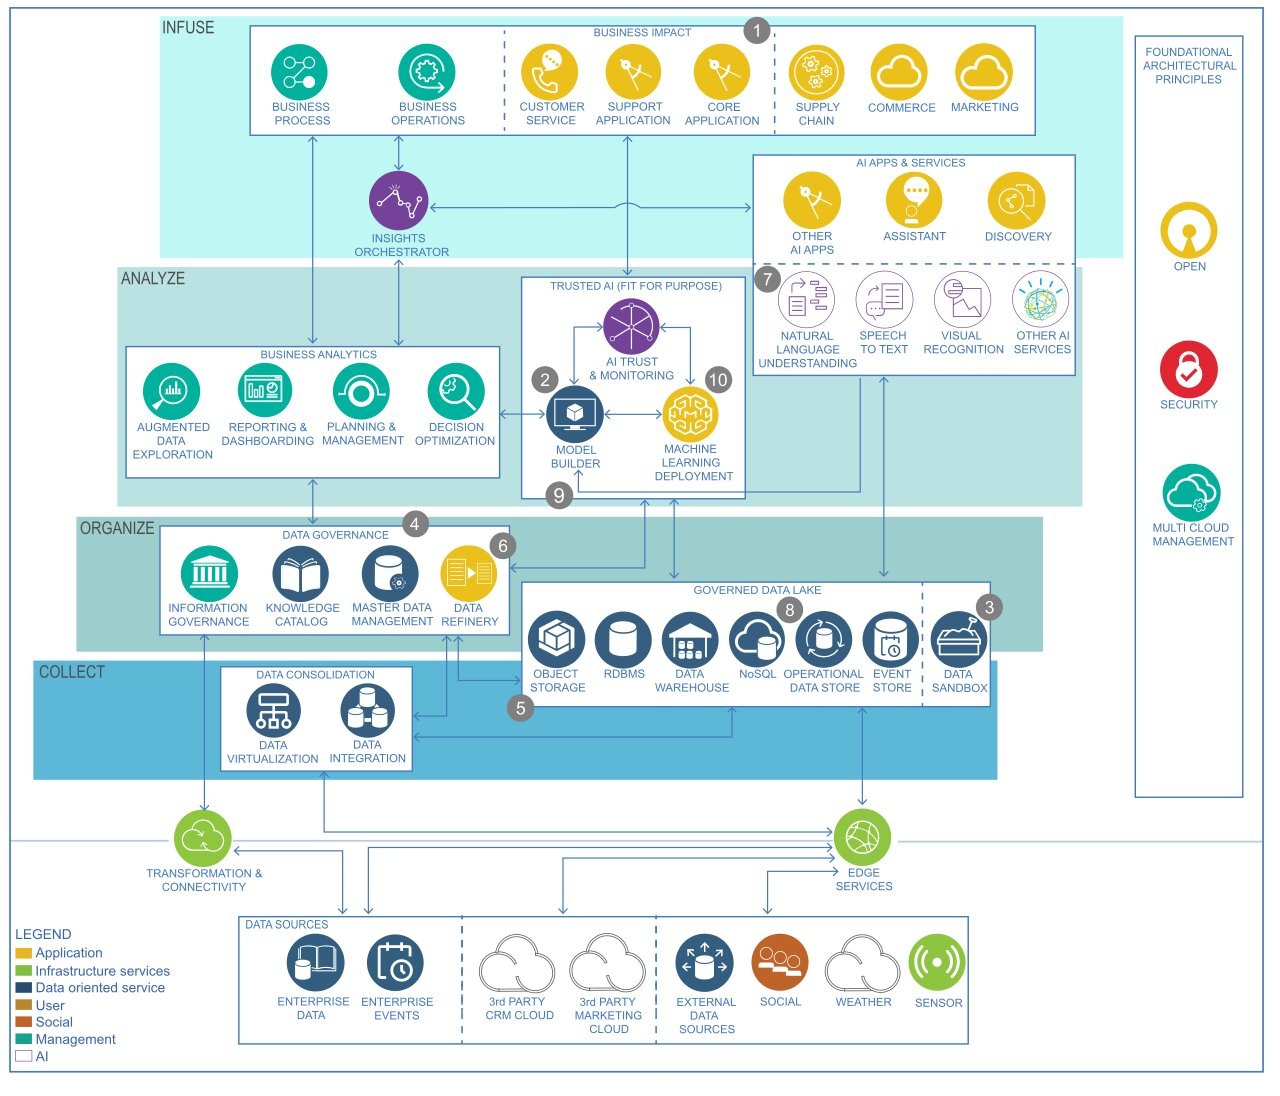
\includegraphics[scale=0.25]{images/ai-analytics-ref-diagram-analyze.jpg}
\caption {IBM Analytics and AI Reference Architecture.}
\label{fig:AIReferenceArchitecture}
\end{figure}

\begin{itemize}
\item \textbf{Coleta:} Relaciona os processos de coleta, armazenamento e transformação de diversas fontes de dados, estruturadas ou não estruturadas, para determinados repositórios (\textit{Data Lakes}).
\item \textbf{Organização:} Relaciona os processos de organização e estruturação dos dados nos presentes nos \textit{Data Lakes} e necessários para o uso das aplicações que envolvem a análise dos dados. Dependendo do uso pode-se aplicar processos de Governança.
\item \textbf{Análise:} Relaciona os processos para desenvolvimento de aplicações de IA e relatórios após a organização dos dados para tomadas de decisão e uso de aplicações externas.
\item \textbf{Infusão:} Relaciona os processos de disponibilização desses dados e conhecimento obtidos na fase de análise para aplicações externas.
\end{itemize}

\section{\textit{ModelOps}}
\label{app:ModelOps}

O ModelOps (ou operacionalização de modelos de IA) está focado principalmente na governança e gerenciamento do ciclo de vida de uma ampla gama de modelos de inteligência artificial (IA) e de decisão operacionalizados, incluindo aprendizado de máquina, grafos de conhecimento, regras, otimização, modelos linguísticos e modelos baseados em agentes~\cite{Gartner_2022}. Os principais recursos incluem integração contínua/entrega contínua (CI/CD), ambientes de desenvolvimento, sistema de controle de versão, armazenamento e reversão de modelos. O termo ModelOps é uma junção de modelos de IA e DevOps, sendo uma nova estrutura e plataforma para gerenciamento completo do ciclo de vida de artefatos de aplicativos de Inteligência Artificial~\cite{Hummer_2019} e cobrindo todos os termos relacionados a implantação de modelos baseados em IA, como MLOps e AIOps. Apesar do termo ModelOps ser criado como a generalização destes termos, a ideia de todos eles é utilizar os princípios de Integração Contínua (CI) e Entrega Contínua (Continuous Delivery, ou CD) presentes no DevOps para garantir que o modelo de IA seja sempre o melhor e mais próximo do cenário que aborda.

\begin{figure}[H]
\centering
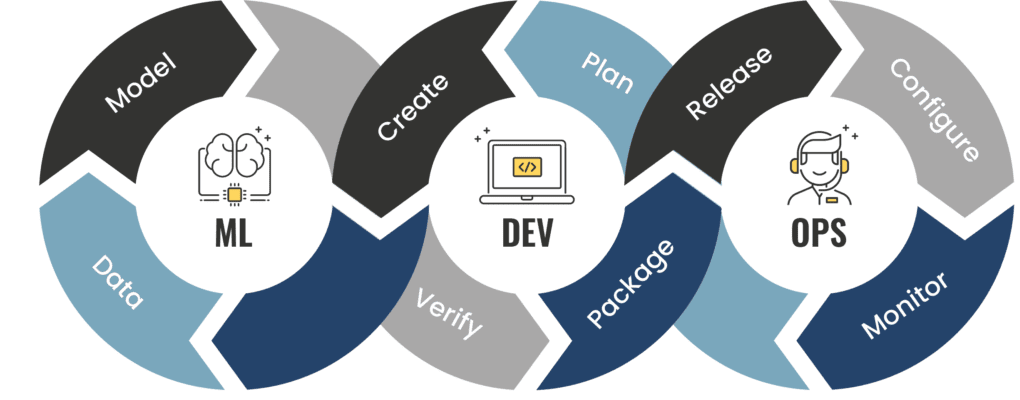
\includegraphics[scale=0.7]{images/code-validate-deploy-loop.png}
\caption {Ciclo resumido do processo presente em MLOps}
\label{fig:MLOpsLoop}
\end{figure}

A operacionalização dos procedimentos em Software já é uma prática comum de ser adotada, mas em aplicações de IA sua adoção é mais recente, e possuem desafios diferentes de uma aplicação tradicional de Software~\cite{Sculley_2015}:

\begin{itemize}
    \item \textbf{Complexidade dos modelos implantados:} A prática tradicional de Engenharia de Software mostrou que o uso de encapsulamento e design modular ajudam a criar código sustentável no qual é fácil de fazer isoladamente mudanças e melhorias. Tais práticas ajudam a expressar a consistência das entradas e saídas de informações de um determinado componente. Infelizmente, é difícil traduzir estas abstrações para sistemas de IA prescrevendo um comportamento pretendido específico. De fato, IA é necessária exatamente nos casos em que o comportamento desejado não pode ser efetivamente expresso na lógica do Software sem dependência de dados externos. O mundo real não se encaixa totalmente de forma encapsulada.
    \item \textbf{Dependência dos dados:} Débito de dependência é apontado como um dos principais contribuintes para a complexidade do código e débito técnico em configurações clássicas de Engenharia de Software. As dependências de dados em sistemas de IA possuem uma capacidade semelhante para aumentar o débito, mas podem ser mais difíceis de detectar. As dependências de código podem ser identificadas por meio de análise estática por compiladores e vinculadores. Sem ferramentas semelhantes para dependências de dados, não é difícil construir grandes cadeias de dependências de dados que podem ser difíceis de arrumar.
    \item \textbf{Ciclos de \textit{Feedback}:} Uma das principais características dos sistemas de IA é que eles geralmente acabam influenciando seu próprio comportamento se forem atualizados ao longo do tempo. Isso leva a uma forma de análise do débito, na qual é difícil prever o comportamento de um determinado modelo antes de ele ser lançado. Esses ciclos de feedback podem assumir diferentes formas, mas são mais difíceis de detectar e resolver se ocorrerem gradualmente ao longo do tempo, como pode ser o caso quando os modelos são atualizados com pouca frequência.
    \item \textbf{\textit{Anti-Patterns} nas aplicações:} É comum que sistemas de IA acabem com grandes débitos em padrões de design. Débitos como \textit{glue code} (integração de sistemas teoricamente incompatíveis), \textit{pipeline jungles} (\textit{pipelines} de grande complexidade e com difícil rastreamento de problemas, geralmente com etapas fortemente acopladas), código não utilizado, débitos de abstração, \textit{code smells} (códigos que podem indicar problemas subjacentes em um componente ou sistema) devem ser evitados ou refatorados sempre que possível.
    \item \textbf{Débitos de configuração:} Qualquer sistema grande tem uma ampla gama de opções configuráveis, incluindo quais \textit{features} são usadas, como os dados são selecionados, uma ampla variedade de configurações de aprendizado específicas de algoritmos, potencial pré ou pós-processamento, métodos de verificação, entre outras. A grande quantidade de opções e a relação que essas tem umas com as outras no sistema torna a configuração difícil de modificar corretamente e difícil de raciocinar. No entanto, erros na configuração podem custar caro, levando a sérias perdas de tempo, desperdício de recursos de computação ou problemas de produção.
    \item \textbf{Mudanças do mundo externo:} Sistemas de IA geralmente interagem diretamente com o mundo externo, e este raramente é estável, criando um custo de manutenção contínuo. Para isso, é importante prever os vieses e determinar limiares para as previsões que estes sistemas irão realizar.
    \item \textbf{Testagem e fidelidade dos dados:} Embora estejam relacionados a itens já mencionados (dependência dos dados e mudanças do mundo externo), a garantia de que estes desafios estejam bem controlados começa durante o desenvolvimento dos modelos. Dados de entrada testados e fidedignos às situações presentes do mundo garantem este controle, e procedimentos para realizar esta tarefa constituem em outro desafio para garantia da qualidade da aplicação.
    \item \textbf{Processos e cultura do time:} É importante criar equipes que se importem na melhora do modelo e do seu próprio processo de implantação. Sistemas maduros podem ter dezenas ou centenas de modelos rodando simultaneamente, tornando-se complexos ao longo do tempo e necessitando de melhoria contínua dos processos para manter a qualidade.
\end{itemize}

No caso de MLOps, ele pode ser visto como o processo de implantar os melhores modelos latentes de Machine Learning para o ambiente de produção, unindo os campos de Machine Learning, DevOps e Engenharia de Dados. Um projeto de MLOps, como exemplo mostrado na Figura \ref{fig:MLOpsPipeline}, deve dar suporte à automação, integração e monitoramento em todas as etapas da construção de um sistema de ML, incluindo treinamento, integração, teste, lançamento, implantação e gerenciamento de infraestrutura~\citep{Testi_2022}. A ideia é projetar um pipeline automatizado usando o CI/CD, sendo a tarefa de CI de testar e validar dados, esquemas de dados e modelos, e a tarefa de CD um pipeline de ML que deve implantar automaticamente outro modelo de ML.

\begin{figure}[H]
\centering
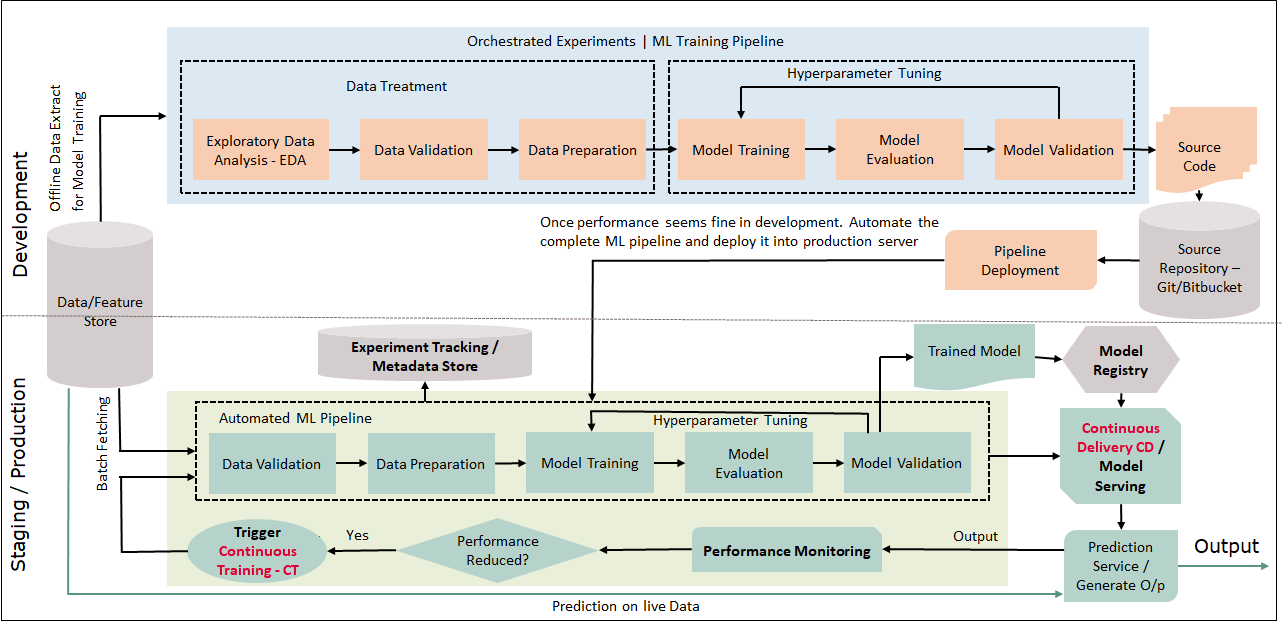
\includegraphics[scale=0.33]{images/mlops-pipeline-example.png}
\caption {Exemplo de Pipeline de MLOps com ambientes de Desenvolvimento e Produção}
\label{fig:MLOpsPipeline}
\end{figure}

O ciclo de vida de Machine Learning tem metodologias diferentes para se adequar a diferentes cenários e tipos de dados. A abordagem mais utilizada por especialistas em mineração de dados é o Cross-Industry Standard Process for Data Mining (CRISP-DM)~\citep{Shearer_2000}, introduzido em 1996 pela Daimler Chrysler. Especialistas podem emprestar as metodologias CRISP-DM padrão e tentar aplicá-las ao pipeline de MLOps, envolvendo dois papeis: Os Cientistas de Dados, responsáveis pelo treinamento e teste do modelo, e os Engenheiros de Machine Learning, responsáveis pela produção e implantação. Tais papeis trabalhariam em conjunto em tarefas envolvendo as seguintes etapas:

\begin{itemize}
    \item Análise do problema do Negócio
    \item Atributos e armazenamento do conjunto de dados
    \item Metodologia analítica de ML
    \item Componentes de um Pipeline de CI
    \item Componentes de um Pipeline de CD
    \item Acionamento automatizado do Pipeline
    \item Armazenamento de registro de modelo
    \item Monitoramento e desempenho
    \item Serviço para implantação de modelos ML em Produção
\end{itemize}

Isso pode ser feito por uma aplicação própria para realizar este gerenciamento, por funcionalidades implementadas na própria aplicação de IA ou através de frameworks de automação como o Amazon SageMaker, que podem poupar tempo para desenvolvimento de uma nova aplicação a troco de um pagamento de acordo com a demanda utilizada. Estes frameworks podem cuidar de toda a parte de gerenciamento dos dados, modelagem/treinamento ou operação/implantação, e como são modulares e cuidam apenas de uma destas três categorias do processo, podem ser escolhidas ou não de acordo com a necessidade do projeto e conhecimento da equipe.

\section{Trabalhos Relacionados}

Os principais trabalhos encontrados envolvendo métricas de \textit{Fairness} e arquitetura de sistemas pensando em \textit{Fairness} como requisito vêm do time de engenharia do LinkedIn.~\citet{Geyik_2019} fala sobre quais métricas foram utilizadas e quais algoritmos foram implementados para ranqueamento dos dados.~\citet{Kenthapadi_2019} fala sobre como o conceito de \textit{Fairness} pode ser implementado em uma aplicação de IA, e mostra a arquitetura sobre ela.

Quanto ao desenvolvimento do \textit{Workflow} e arquiteturas, é possível mencionar a própria IBM AI Reference Architecture~\citep{IBM_2021} como modelo para desenvolvimento de aplicações. Uma outra arquitetura que é comparável a arquitetura \textit{Pipes-and-Filters} é a FBFlow do Facebook~\citep{Dunn_2016}. O uso de DAGs (\textit{Direct Acyclic Graphs}) para a execução de um determinado processo ou \textit{workflow} é uma alternativa simples de ser implementada e interpretada pelos desenvolvedores, onde é possível conectar o método de ML juntamente com o cálculo de métricas para serem automatizados e organizados de forma simultânea. Há diferenças entre DAGs e \textit{pipes} e filtros, mas o objetivo de ambos acaba sendo o mesmo: Conectar diversos processos menores para formar um sistema coeso. Também por este trabalho de mestrado se tratar de um \textit{Workflow} focando em diversos algoritmos envolvendo redução de vieses, estes mesmos algoritmos, apresentados no capítulo \ref{sec:unbiasedAlgorithms}, também podem ser considerados como parte de trabalhos relacionados.

Quanto ao desenvolvimento da parte que utiliza o MAPE-K para garantir a autonomia, já há diversos artigos detalhando como o MAPE-K é importante para organizar o processo de decisão, como o \textit{"An architectural blueprint for autonomic computing"}~\citep{IBM_2005}, que detalha todas as suas bases. Para o desenvolvimento da parte de análise, um trabalho que pode ser mencionado é o artigo \textit{"The VADA Architecture for Cost-Effective Data Wrangling"}~\citep{Konstantinou_2017}, que utiliza pesos para dar contexto aos dados medidos. Embora não seja o principal tema do artigo, indicar a importância dos dados analisados garantiu a autonomia necessária sem exigir manutenção na parte de análise.

Outro trabalho a ser mencionado é o artigo \textit{"The ML test score: A rubric for ML production readiness and technical debt reduction"}~\citep{Breck_2017}, que usa uma pontuação aplicando questionários usando diversos fatores para determinar a saúde de um projeto de IA. Embora o questionario seja manual e o foco esteja na saúde do projeto ao invés da determinação dos algoritmos para a construção de melhores modelos, o cerne do que foi utilizado como solução é o mesmo: O uso de uma pontuação como garantia de melhora contínua.

\begin{table}[h]
\begin{center}
  \resizebox{\linewidth}{!}{%
  \begin{tabular}{cccccccccc}
    \toprule
    \multicolumn{2}{c}{\multirow{2}{*}{\bf Referências}} & \multicolumn{2}{c}{\multirow{2}{*}{\bf Descrição}} & \multicolumn{6}{c}{Conceitos}\\
    \cmidrule{5-10}
%    \hline
    \multicolumn{4}{c}{} & \bf Ciência/Eng. Dados & \bf ML & \bf Fairness & \bf Eng. Software & \bf Prov. dados & \bf Arq. Software\\
    \midrule
    \multicolumn{2}{c}{Geyik et al., 2019} & \multicolumn{2}{c}{\makecell{Métricas utilizadas \\ Ranqueamento dos dados}} &  & \cmark & \cmark & \cmark &  & \\[3ex]
%    \hline
    \multicolumn{2}{c}{Kenthapadi et al., 2019} & \multicolumn{2}{c}{Arquitetura/implementação de métricas de Fairness} &  & \cmark & \cmark & \cmark &  & \\[2ex]
%    \hline
    \multicolumn{2}{c}{\makecell{IBM Analytics and \\ AI Reference Architecture}} & \multicolumn{2}{c}{\makecell{Arquitetura de referência para Dados e ML}} & \cmark & \cmark &  & \cmark &  & \\[3ex]
%    \hline
    \multicolumn{2}{c}{\makecell{An architectural blueprint \\ for autonomic computing}} & \multicolumn{2}{c}{\makecell{Arquitetura para sistemas autônomos}} &  &  &  & \cmark &  & \cmark\\[3ex]
%    \hline
    \multicolumn{2}{c}{\makecell{FBFlow - Facebook \\ (Dunn, 2016)}} & \multicolumn{2}{c}{\makecell{Uso de DAGs para determinar \textit{workflow} \\ Execução/interpretação de processos de ML}} &  & \cmark & \cmark & \cmark &  & \cmark\\
%    \hline
    \multicolumn{2}{c}{\makecell{Konstantinou et al.,2017}} & \multicolumn{2}{c}{\makecell{Arquitetura para entrelaçamento de dados \\ Utilização de pesos para determinar contexto aos dados}} & \cmark &  &  &  & \cmark & \cmark\\[3ex]
%	\hline    
    \multicolumn{2}{c}{\makecell{Breck et al.,2017}} & \multicolumn{2}{c}{\makecell{Questionários para determinar pontuações em projetos de ML \\ Saúde e qualidade do projeto como fatores medidos}} & \cmark & \cmark &  & \cmark &  & \\[3ex]    
    \bottomrule
  \end{tabular}}
\end{center}
\end{table}

\chapter{Metodologia}
\label{sec:metodologia}

\section{Detalhamento do processo}

Com base nas etapas da AI Reference Architecture, foram definidos para este trabalho os seguintes papeis onde um projeto de Machine Learning pode ter atuação e onde se encaixariam:

\begin{itemize}
\item \textbf{Especialista de Domínio:} É a pessoa que detém de todo o conjunto de regras do qual a aplicação deve respeitar. Pode não ter conhecimento técnico, embora esse conhecimento possa ajudar na comunicação das regras com os demais papeis. Está presente nas fases de Coleta, Organização e Infusão do ciclo.

\item \textbf{Engenheiro de Dados:} É a pessoa responsável pelos processos de coleta e transformação dos dados para o uso em outros processos, sejam eles de Softwares tradicionais ou aplicações de Machine Learning. Pode aplicar processos de governança antes de definir que o dado esteja pronto para ser usado por outras pessoas. Está presente nas fases de Coleta e Organização do ciclo.

\item \textbf{Cientista de Dados:} É a pessoa responsável pela análise dos dados e do desenvolvimento do processo de Machine Learning após a transformação e tratamento dos dados. Pode realizar tratamentos próprios antes do treinamento, como \textit{Encoding} (\textit{Label Encoding}/\textit{One-hot Encoding}), normalização, processos de regularização como aumentação de dados, para melhorar a performance do mesmo. Está presente nas fases de Organização e Análise do ciclo.

\item \textbf{Engenheiro de Software:} É a pessoa responsável por usar o modelo de Machine Learning obtido na fase de Análise em aplicações que façam sentido para seu uso, como assistentes, automações, dashboards e relatórios. Está presente apenas na fase de Infusão, mas pode ser considerado na fase de Análise para verificar com o Cientista de Dados como está o andamento dos modelos desenvolvidos e desenhar alternativas caso os mesmos não estejam prontos para uso.

\end{itemize}

O desenvolvimento realizado neste trabalho pode ser dividido em 5 etapas maiores, que podem ser detalhadas e sub-divididas:

\begin{itemize}
\item \textbf{Obtenção dos conjuntos de dados:} Foi realizada uma pesquisa para verificar quais os conjuntos de dados utilizados em experimentos de artigos acadëmicos envolvendo algoritmos de redução de vieses. Após a pesquisa, alguns foram selecionados e obtidos para os experimentos deste trabalho.

\item \textbf{Transformação dos conjuntos de dados (Engenharia de Dados):} Como alguns dos conjuntos de dados obtidos diferentes valores qualitativos e codificados de acordo com o atributo, primeiro foi realizado uma transformação dos dados para garantir uma melhor legibilidade, o que já equivaleria minimamente ao trabalho do Engenheiro de Dados presente neste trabalho de Mestrado. Posteriormente, novas transformações foram realizadas devido a necessidade de separar grupo privilegiado ao grupo não-privilegiado, mas neste trabalho já equivaleria a parte do Cientista de Dados.

\item \textbf{Desenvolvimento do Workflow:} Como Machine Learning possui um processo muito bem definido, é possível subdividir este processo em etapas e subdividir cada uma dessas etapas em componentes isolados. O objetivo do desenvolvimento de um \textit{Workflow} é sistematizar todo esse processo de modo que supostas atualizações sejam incrementais e que seja possível realizar uma execução de forma autônoma a partir da próxima etapa. Para simplificar o processo, foi utilizada a arquitetura \textit{Pipes-and-Filters}, que é simples de ser entendida e pode ser encontrada em diferentes publicações.

\item \textbf{Desenvolvimento do Gerenciador Autonômico:} Após o desenvolvimento do \textit{Workflow}, foi desenvolvido um elemento autônomo para trabalhar em conjunto com o \textit{Workflow} como elemento gerenciado. Através das métricas obtidas em execuções anteriores, é possível inferir sugestões de melhores combinações para execução e garantia de um melhor resultado de forma mais eficiente. Para garantir uma maior flexibilidade nos resultados, foram implementadas diversas estratégias para garantir que essa sugestão seja customizada pelo Cientista de Dados e/ou pelo Especialista de Domínio se isso for necessário para as necessidades do problema.

\item \textbf{Interface Humano-Computador:} Para facilitar o entendimento dos arquivos utilizados para configuração e utilização das estratégias da arquitetura MAPE-K, foi criada uma interface onde é possível realizar a configuração pela mesma, podendo também realizar uma execução do \textit{Workflow} isolada e uma execução com sugestões, acompanhando a análise realizada no gerenciador MAPE-K.

\end{itemize}

Dado esses papeis e etapas, foi desenhado um diagrama de atividades, presente na Figura \ref{fig:AIRoles}, determinando como eles se encaixariam no processo. Detalhes de implementação serão explicados na seção \ref{sec:Desenvolvimento}.

\begin{figure}[H]
\centering
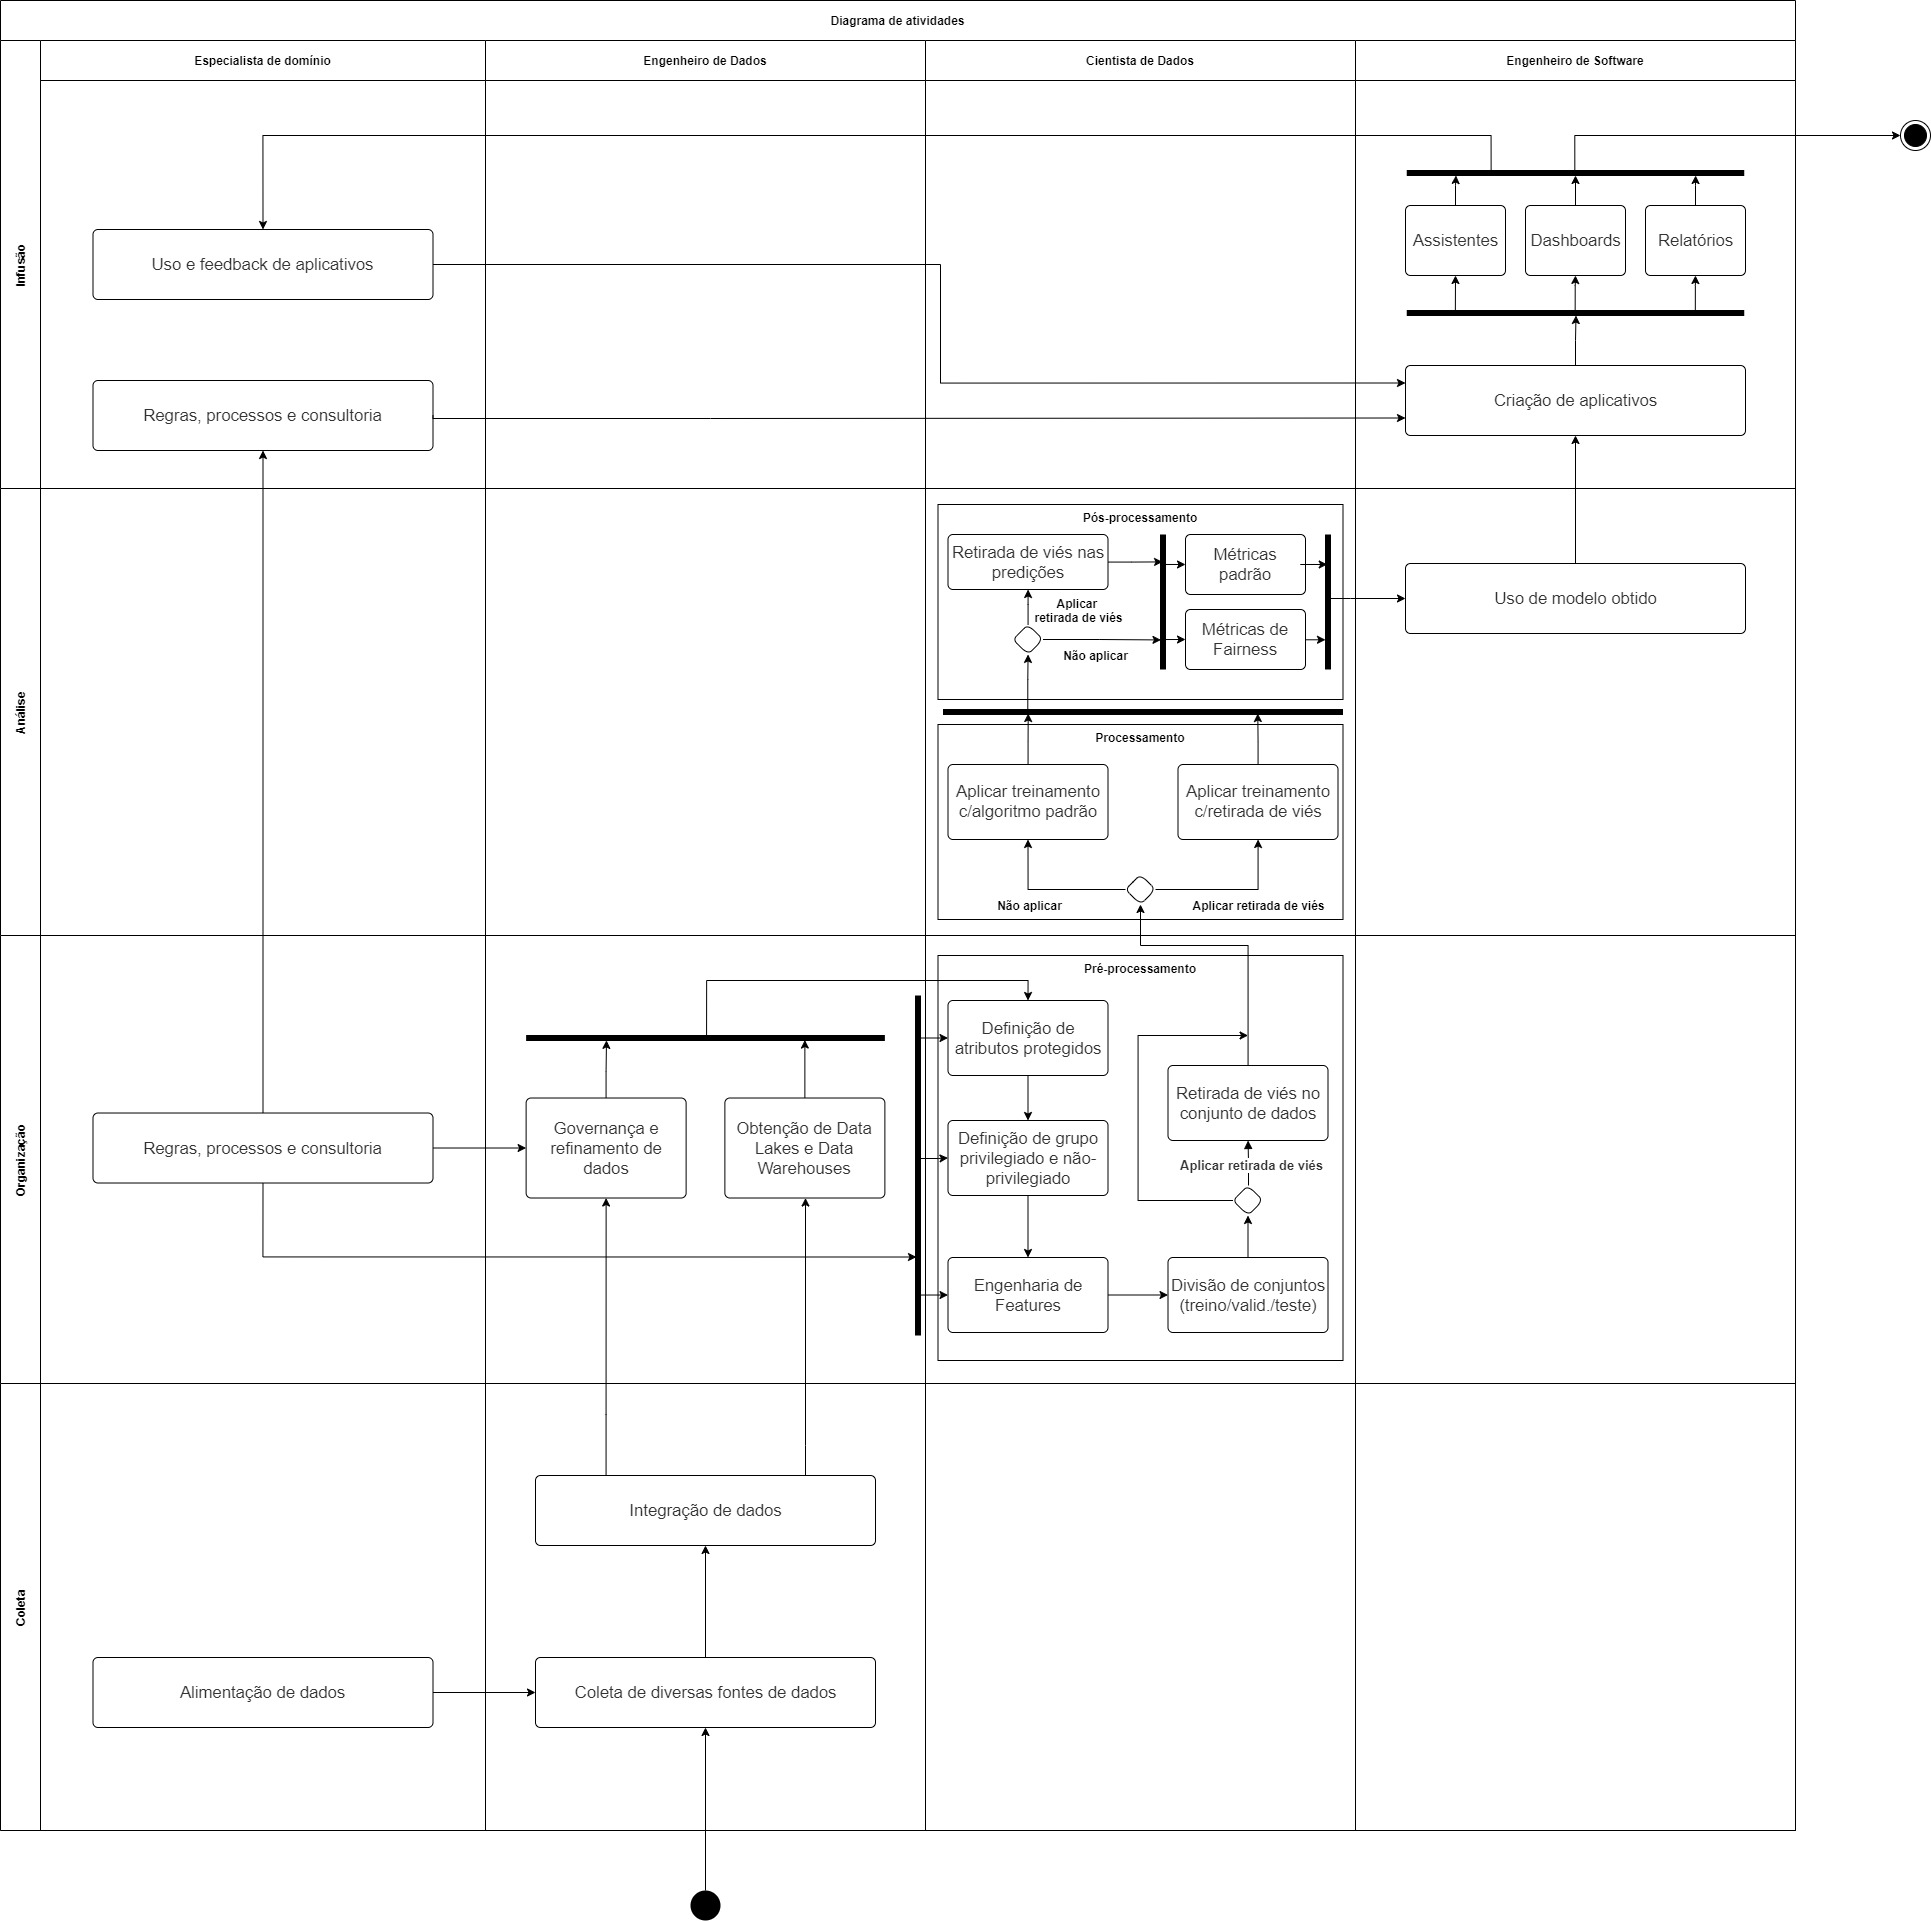
\includegraphics[scale=0.25]{images/Diagrama_Atividades.jpg}
\caption {Diagrama de atividades com subdivisão de cada papel em uma aplicação de IA utilizando métricas de Fairness, com base na IBM AI Reference Architecture~\citep{IBM_2021}}
\label{fig:AIRoles}
\end{figure}

\section{Arquitetura do sistema}

\begin{figure}[h]
\centering
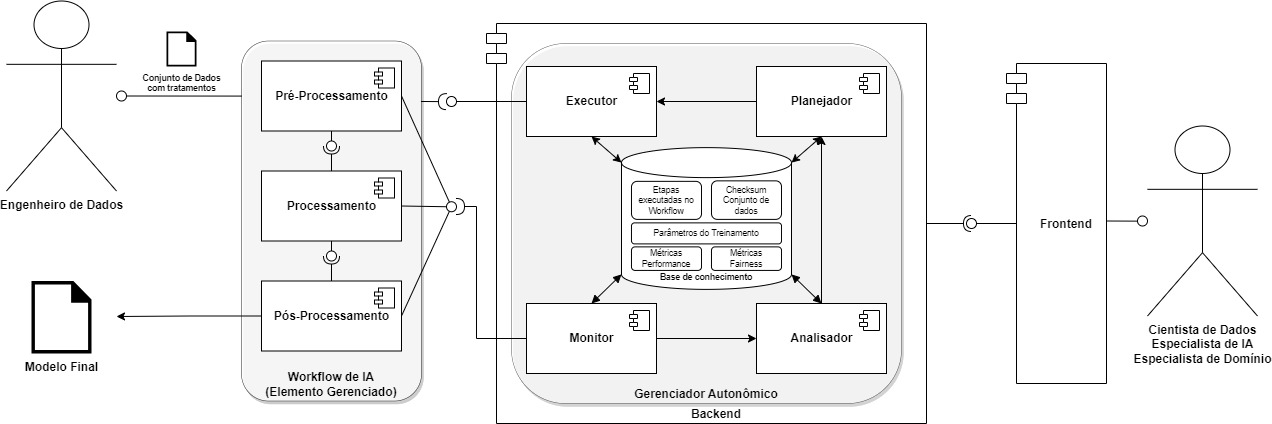
\includegraphics[scale=0.35]{images/backend-frontend-ml.jpg}
\caption {Componentes arquiteturais da solução}
\label{fig:BackendFrontendML}
\end{figure}

\begin{sidewaysfigure}
\clearpage
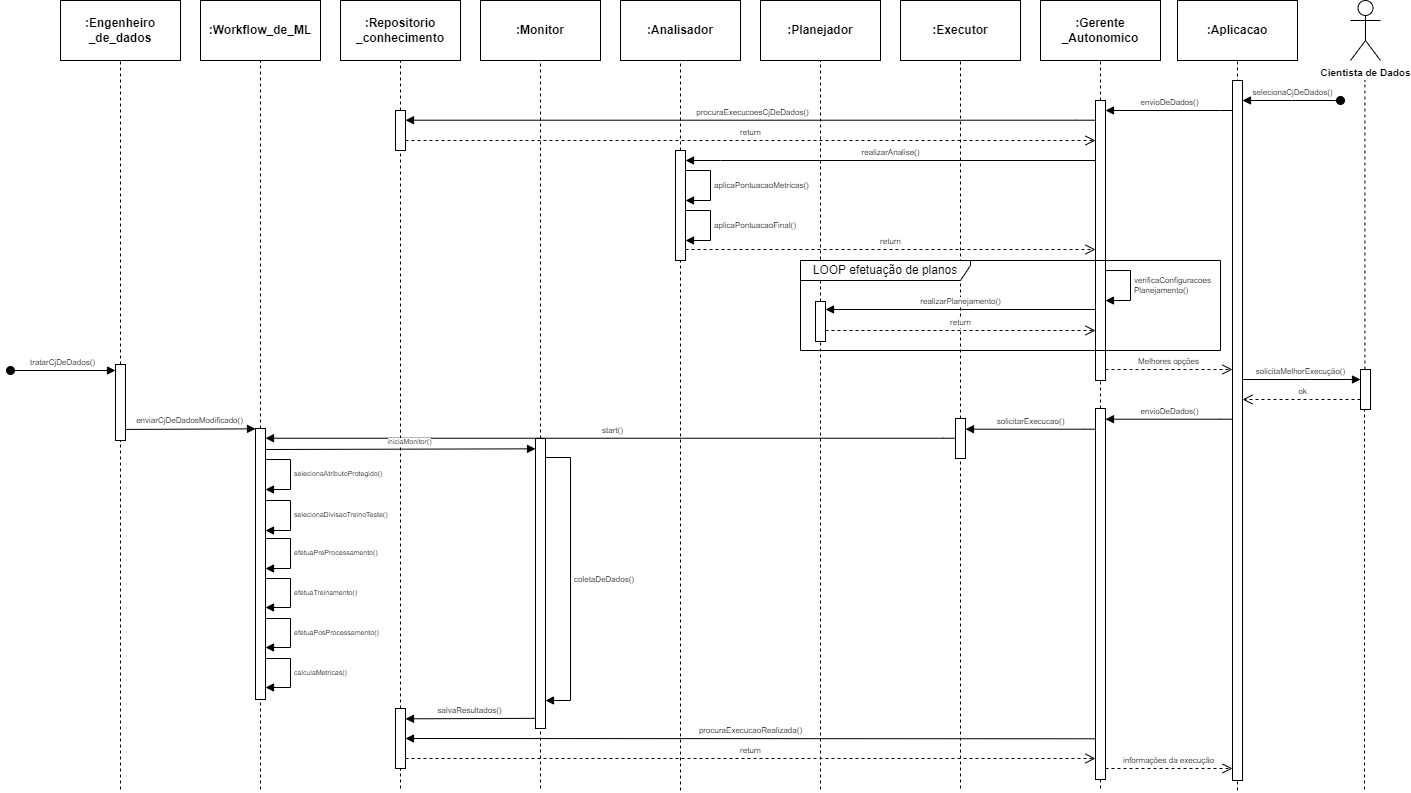
\includegraphics[scale=0.465]{images/Diagrama_Sequencia.jpg}
\caption {Diagrama de sequência do sistema}
\label{fig:DiagramaSequencia}
\end{sidewaysfigure}

Dado as etapas acima, o sistema foi dividido em 5 módulos:

\begin{itemize}
    \item {\textbf{Engenharia de Dados:}} Módulo com o objetivo de executar processos de limpeza e transformação de dados.
	\item {\textbf{\textit{Workflow} de ML:}} Módulo que executa um \textit{Pipeline} capaz de automatizar uma aplicação de ML, com estágios de preparação de dados (Pré-processamento), treinamento (Processamento) e avaliação dos resultados (Pós-processamento) para a geração de um modelo final.
     \item {\textbf{Gerenciador autonômico:}} Módulo contendo um \textit{loop} MAPE-K que controla o \textit{Workflow} como um Elemento Gerenciado para automatizar tais etapas, com o objetivo de evitar execuções manuais dependendo do algoritmo e/ou do conjunto de dados usado nas etapas.
     \item {\textbf{Interface (Frontend):}} Módulo cujo objetivo é prover uma experiência de usuário mais simples e intuitiva para o Cientista de Dados para configurar e iniciar o Gerenciador Autonômico.
	\item {\textbf{Backend:}} Módulo criado com o objetivo de conectar a Interface com o Gerenciador Autonômico.
\end{itemize}

A integração entre esses módulos é ilustrada na Figura \ref{fig:BackendFrontendML}. O módulo de Engenharia de Dados é usado pelo Engenheiro de Dados, que retorna um conjunto de dados com os tratamentos necessários para execução do \textit{workflow}. A Interface será utilizada pelo Cientista de Dados, que determinaria as configurações necessárias dependendo do contexto do problema. 

O processo que ocorre, desde a interação da interface, passando pela execução do \textit{Workflow} e chegando na obtenção dos resultados, pode ser visualizado no Diagrama de Sequência presente na Figura \ref{fig:DiagramaSequencia}. Neste processo, enquanto o Engenheiro de dados manipula o conjunto de dados com os processos de limpeza e transformação de dados presentes no módulo de Engenharia de Dados e envia estes conjuntos modificados para integração e uso no \textit{Workflow} de ML, o Cientista de Dados, pelo módulo de Interface presente na aplicação, escolhe o Conjunto de Dados e solicita uma execução do Gerenciador Autonômico. O Gerenciador Autonômico busca todas as execuções já realizadas no \textit{Workflow} de ML que já utilizaram o conjunto de dados modificado e estão salvas na Base de Conhecimento, fará a análise realizando cálculos que serão detalhados posteriormente, e fará um \textit{loop} verificando a configuração de planos de execução já implementados e executando em seguida, retornando as melhores opções de execução para que o Cientista de Dados escolha a opção mais adequada e requisitar uma nova execução para o \textit{Workflow} de ML. Durante a requisição, o \textit{Workflow} de ML inicia o Monitor do Gerenciador Autonômico para coletar dados durante a execução, seleciona o conjunto de dados e seu atributo protegido, realiza a divisão entre conjuntos de treino e teste, executa os algoritmos nas etapas de Pré-processamento, Processamento and Pós-processamento, e calcula as métricas do modelo final. O Monitor salva todos os dados coletados na Base de Conhecimento, e o Gerenciador Autonômico busca os dados desta execução para exibição na Interface ao Cientista de Dados.

\section{Desenvolvimento}
\label{sec:Desenvolvimento}

\subsection{Engenharia de Dados}

Nesta etapa, os conjuntos de dados obtidos com atributos qualitativos codificados com uma documentação própria, como o \textit{German Credit Dataset}~\citep{ucigerman_2021}, são transformados com nomenclaturas mais legíveis e colocados em arquivos CSV. O Trecho \ref{cod:DataEngTransform}, colocado abaixo, ilustra um exemplo dessas operações.

\begin{lstlisting}[language=Python, caption=Transformações do conjunto de dados \textit{German Credit Dataset},label=cod:DataEngTransform]
def german_data_to_csv():
    pd.set_option('display.max_columns', None)
    df = pd.read_csv('datasets/german.data', sep=' ')
    df.info()
    print(df)

    df['checking_account'] = df['checking_account'].map(
        {'A11': '<0', 'A12': '0<=x<200', 'A13': '>=200', 'A14': 'None'}).astype(str)
    df['credit_history'] = df['credit_history'].map(
        {'A30': 'no_credits_taken', 'A31': 'all_credits_paid_bank',
         'A32': 'existing_credits_paid', 'A33': 'delay_in_past', 'A34': 'critical'}).astype(str)
    df['purpose'] = df['purpose'].map( 'radio/tv',
         'A44': 'domestic_appliances', 'A45': 'repairs', 'A46': 'education', 'A47':
        {'A40': 'car_new', 'A41': 'car_used', 'A42': 'furniture/equipment', 'A43': 'vacation', 'A48': 'retraining',
         'A49': 'business', 'A410': 'others'}).astype(str)
    df['savings_account'] = df['savings_account'].map(
        {'A61': '<100', 'A62': '100<=x<500', 'A63': '500<=x<1000', 'A64': '>=1000', 'A65': 'unknown'}).astype(str)
    df['present_employment_since'] = df['present_employment_since'].map(
        {'A71': 'unemployed', 'A72': '<1', 'A73': '1<=x<4', 'A74': '4<=x<7', 'A75': '>=7'}).astype(str)
    df['personal_status_sex'] = df['personal_status_sex'].map(
        {'A91': 'male_divorced/separated', 'A92': 'female_divorced/separated/married', 'A93': 'male_single',
         'A94': 'male_married/widowed', 'A95': 'female_single'}).astype(str)
    df['other_debtors_guarantors'] = df['other_debtors_guarantors'].map(
        {'A101': 'None', 'A102': 'co-applicant', 'A103': 'guarantor'}).astype(str)
    df['property'] = df['property'].map(
        {'A121': 'real_estate', 'A122': 'savings_insurance', 'A123': 'car_other', 'A124': 'unknown'}).astype(str)
    df['installment_plans'] = df['installment_plans'].map(
        {'A141': 'bank', 'A142': 'stores', 'A143': 'None'}).astype(str)
    df['housing'] = df['housing'].map(
        {'A151': 'rent', 'A152': 'own', 'A153': 'for_free'}).astype(str)
    df['job'] = df['job'].map(
        {'A171': 'unemployed', 'A172': 'unskilled', 'A173': 'skilled', 'A174': 'management'}).astype(str)
    df['telephone'] = df['telephone'].map(
        {'A191': 'none', 'A192': 'yes'}).astype(str)
    df['foreign'] = df['foreign'].map(
        {'A201': 'yes', 'A202': 'no'}).astype(str)
    df['risk'] = df['risk'].map(
        {1: 'good', 2: 'bad'}).astype(str)

    print(df)
    df.to_csv('datasets/german_credit_data.csv')
\end{lstlisting}

Nele, cada uma das colunas presentes no conjunto de dados que atribuem uma qualidade é renomeada de acordo com o equivalente presente em sua documentação. Esta etapa simularia uma transformação realizada por um Engenheiro de Dados para facilitar o trabalho de análise e implementação de um Cientista de Dados.

\subsection{Workflow}

\subsubsection{Desenvolvimento de \textit{Framework}}

Para facilitar o desenvolvimento do \textit{Workflow} e deixar seu código mais legível, foi vista durante seu desenvolvimento a necessidade de desenvolver um pequeno \textit{Framework} baseado na arquitetura \textit{Pipes-and-Filters} onde foram feitas adaptações devido a características e a limitações da linguagem \textit{Python}.

\begin{figure}[H]
\centering
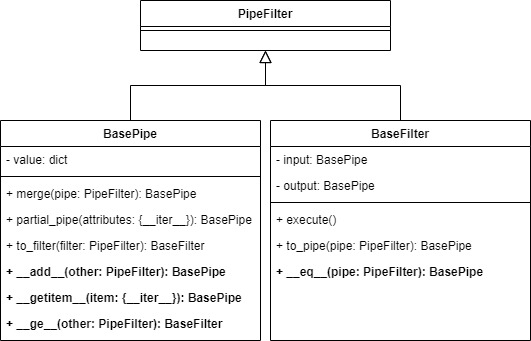
\includegraphics[scale=0.8]{images/classdiagram_Pipe-and-Filter_framework.jpg}
\caption {Diagrama de classes do \textit{Framework} baseado na arquitetura \textit{Pipes-and-Filters}}
\label{fig:PipeAndFilterFramework}
\end{figure}

Conforme ilustrado na Figura \ref{fig:PipeAndFilterFramework}, o \textit{Framework} possui 3 classes: \textbf{PipeFilter}, \textbf{BasePipe} e \textbf{BaseFilter}. A classe \textbf{PipeFilter} foi criada para ser herdada pelas classes \textbf{BasePipe} e \textbf{BaseFilter} por duas limitações: Inexistência de interfaces no \textit{Python} e acusação de heranças cíclicas. A classe \textbf{BasePipe} possui apenas um atributo \textbf{value} que é um dicionário que simboliza os dados que trafegam por esse Pipe. Como é um dicionário, ele é totalmente livre de quantos atributos o Pipe trafega, sendo assim a sua validação é responsabilidade da aplicação. A classe \textbf{BaseFilter} possui dois atributos \textbf{input} e \textbf{output} que simbolizam os Pipes de entrada e de saída do Filtro, e o uso desses dois Pipes mais a execução do Filtro vai estruturar o \textit{Workflow} como um todo.

O \textit{Workflow} é realizado através de encadeamentos do método \textbf{to\_filter} com o método \textbf{to\_pipe}. O método \textbf{to\_filter} prepara um Filtro para utilizar o Pipe, setando o atributo \textbf{input} presente na classe de Filtro passada como parâmetro, e o método \textbf{to\_pipe} obtém o Pipe resultante do Filtro, chamando o método \textbf{execute} e obtendo o atributo \textbf{output} presente no Filtro para setar no atributo \textbf{value} presente na classe de Pipe passada como parâmetro. Isso forma encadeamentos de métodos que se assemelham muito com os de uma \textit{Fluent API}~\citep{Fowler_2005}, criando uma DSL (\textit{Domain-Specific Language}) cujo domínio é a estruturação de um \textit{Workflow}. Como os métodos \textbf{to\_filter} e \textbf{to\_pipe} recebem um parâmetro do tipo \textbf{PipeFilter} devido ao problema de herança cíclica, uma validação de tipo é realizada via código para prosseguir com o tipo correto. O Trecho \ref{cod:PipeAndFilterMethods} mostra um breve exemplo de como é possível encadeá-los, onde \textbf{Pipe1}, \textbf{Pipe2} e \textbf{Pipe3} são classes que herdam \textbf{BasePipe} e \textbf{Filter1} e \textbf{Filter2} são classes que herdam \textbf{BaseFilter}.

\begin{lstlisting}[language=Python, caption=Exemplo de uso do \textit{Framework} para encadeamento dos Workflows,label=cod:PipeAndFilterMethods]
root_pipe = Pipe1()

pipe_with_filter_transformations = root_pipe.to_filter(Filter1())
											.to_pipe(Pipe2())
											.to_filter(Filter2())
											.to_pipe(Pipe3())
\end{lstlisting}

Como a execução dos próprios filtros já é executada dentro do método \textbf{to\_pipe}, basta apenas realizar a instância das classes e executar os métodos \textbf{to\_filter} e \textbf{to\_pipe} para a execução do \textit{workflow}. Com isso, os algoritmos de Machine Learning ficam encapsulados em classes que herdam a classe \textbf{BaseFilter} e utilizam o método \textbf{execute} para executá-los. Desta forma, acontece a separação de interesses entre o componente que gerencia a execução do \textit{Workflow} e os componentes que gerenciam cada passo do \textit{Workflow} especificamente, garantindo um baixo acoplamento entre os componentes uma vez que é possível trocar de componentes que executam diferentes métodos sem afetar a execução do \textit{Workflow}. Consequentemente, conforme novos métodos são descobertos, adicioná-los ao \textit{Workflow} é extremamente simples e envolve poucas mudanças no código original. Ferramentas como o Apache Airflow~\citep{ApacheAirflow_2022} realizam uma abordagem semelhante através da classe \textbf{BaseOperator}, que pode ser herdada para implementar um operador customizado e executá-lo através de DAGs (\textit{Direct Acyclic Graphs})

Utilizando o recurso de métodos especiais presente no Python~\citep{Pyspmethods_2022}, é possível manipular alguns \textit{tokens} como \textit{proxies} para executar os métodos já presentes no \textit{Framework}, simplificando a DSL e também simplificando o entendimento do \textit{Workflow} caso o Cientista de Dados tenha ciência do recurso. Para o método \textbf{to\_filter} foi escolhido o \textit{token} \textbf{$>$=}, pela semelhança com um funil, que é geralmente assemelhado a filtros em sistemas atuais, e para o \textit{token} o método \textbf{\_\_ge\_\_} é implementado como um \textit{proxy} do mesmo. Para o método \textbf{to\_pipe} foi escolhido o \textit{token} \textbf{==}, pela semelhança com um cano (pipe, em inglês), e para este \textit{token} o método \textbf{\_\_eq\_\_} é implementado como um \textit{proxy}.

\begin{lstlisting}[language=Python, caption=Trecho \ref{cod:PipeAndFilterMethods} adaptado com métodos especiais da linguagem \textit{Python},label=cod:PipeAndFilterSpecialMethods]
root_pipe = Pipe1()

pipe_with_filter_transformations = root_pipe >= Filter1() == Pipe2() >= Filter2() == Pipe3()
\end{lstlisting}

Também foram implementados métodos para manipular os dicionários presentes nos Pipes conforme necessário. O método \textbf{merge(pipe)} junta os atributos presentes nos dicionários dos Pipes em um único Pipe, enquanto o método \textbf{partial\_pipe(attributes)} pega apenas os atributos presentes nos dicionários dos Pipes que forem especificados em uma lista de atributos definida no parâmetro \textbf{attributes}, conforme ilustrado no Trecho \ref{cod:PipeAndFilterManipulation}.

Para o método \textbf{merge} foi escolhido o \textit{token} \textbf{+}, pela semelhança com uma operação de adição, e para este \textit{token} o método \textbf{\_\_add\_\_} é implementado como um \textit{proxy}. E para o método \textbf{partial\_pipe} foi escolhido os \textit{tokens} \textbf{[]}, colocados após o dicionário, pela semelhança com a operação de procurar com um item no dicionário (neste caso, é possível procurar um ou mais itens), e para este \textit{token} o método \textbf{\_\_getitem\_\_} é implementado como um \textit{proxy}. O Trecho \ref{cod:PipeAndFilterManipulationSpecial} mostra exemplos da modificação.

\begin{lstlisting}[language=Python, caption=Manipulações para Pipes presentes no \textit{Framework},label=cod:PipeAndFilterManipulation]
pipe1 = Pipe1()
pipe1.value = {'attribute1': 1, 'attribute2': 2}

pipe2 = Pipe2()
pipe2.value = {'attribute3': 3, 'attribute4': 4}


pipe3 = pipe1.merge(pipe2)
print(pipe3) # Output - {'attribute1': 1, 'attribute2': 2, 'attribute3': 3, 'attribute4': 4}
pipe4 = pipe3.partial_pipe(['attribute1', 'attribute3'])
print(pipe4) # Output - {'attribute1': 1, 'attribute3': 3}
\end{lstlisting}

\begin{lstlisting}[language=Python, caption=Manipulações para Pipes com métodos especiais,label=cod:PipeAndFilterManipulationSpecial]
pipe1 = Pipe1()
pipe1.value = {'attribute1': 1, 'attribute2': 2}

pipe2 = Pipe2()
pipe2.value = {'attribute3': 3, 'attribute4': 4}


pipe3 = pipe1 + pipe2
print(pipe3) # Output - {'attribute1': 1, 'attribute2': 2, 'attribute3': 3, 'attribute4': 4}
pipe4 = pipe3['attribute1', 'attribute3']
print(pipe4) # Output - {'attribute1': 1, 'attribute3': 3}
\end{lstlisting}

\subsubsection{Arquitetura e desenvolvimento do Workflow}

O \textit{Workflow} segue uma estrutura das fases de Pré-processamento, processamento e pós-processamento presentes em um processo para desenvolvimento de um modelo de Machine Learning, ilustrados na Figura \ref{fig:FairnessPipeline}. Os pontos de decisão entre redução de viés ou não presentes na figura foram colocados para ilustrar melhor onde atuam os algoritmos de redução dos vieses, mas em sua implementação cada algoritmo foi pensado como um componente isolado, podendo ser alterado em sua respectiva fase (Pré-Processamento, Processamento e Pós-Processamento) com uma simples mudança de parâmetro.

Além de tratar os dados, treinar o modelo e realizar testes sobre o mesmo, o \textit{Workflow} possui etapas para obter os metadados durante o processo e salvá-los junto com as métricas para obter os metadados necessários para integrá-lo a um elemento autônomo. Para a execução dos algoritmos com redução de viés, é utilizada a biblioteca AI Fairness 360, ou AIF360~\citep{AIF360_2022}, biblioteca da IBM que compila diversos algoritmos para este fim e facilita o cálculo das métricas de Fairness. Para os algoritmos sem redução de viés, é usado o scikit-learn~\citep{scikit_2022}.

Devido a natureza deste trabalho de Mestrado ser voltada à Engenharia de Software e a métricas de Fairness, detalhes do processo que também poderiam ser utilizados como estratégias mais sofisticadas para validação dos modelos, como \textit{k-fold Cross Validation}, e estratégias para regularização foram desconsiderados para evitar complexidade.

\begin{figure}[H]
\centering
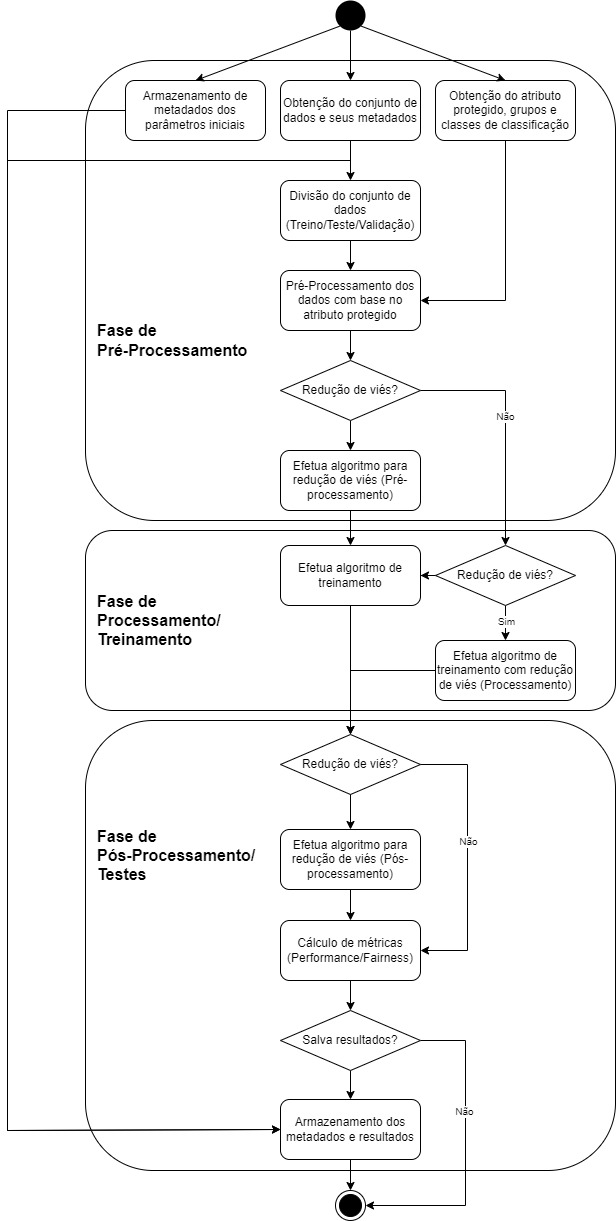
\includegraphics[scale=0.4]{images/ml-fairness-pipeline.jpg}
\caption {Fases e etapas do Workflow implementado}
\label{fig:FairnessPipeline}
\end{figure}

Cada etapa ilustrada na figura se comporta da seguinte maneira:

\begin{itemize}
\item \textbf{Fase de Pré-Processamento:}
	\begin{itemize}
	\item \textbf{Armazenamento de metadados dos parâmetros iniciais:} Os parâmetros que irão determinar quais serão os conjuntos de dados, atributos protegidos e algoritmos utilizados em cada fase do \textit{Workflow} são armazenados em um Pipe e guardados para uma gravação em arquivo caso necessário.
	\item \textbf{Obtenção do conjunto de dados e seus metadados:} De acordo com o parâmetro passado para o \textit{Workflow}, um Pipe relativo ao conjunto de dados em questão é selecionado, e os metadados presentes neste Pipe podem ser utilizados para uma gravação em arquivo caso necessário.
	\item \textbf{Obtenção do atributo protegido, grupos e classes de classificação:}De acordo com o parâmetro passado para o \textit{Workflow}, um Pipe relativo ao atributo protegido em questão é selecionado, e informações de grupos privilegiados e não-privilegiados e classes para classificação, necessárias para executar os algoritmos presentes no AIF360, também estão presentes neste Pipe.
	\item \textbf{Divisão do conjunto de dados (Treino/Validação/Testes):} Um Filtro relativo a divisão do conjunto de dados (entre conjunto de treino, conjunto de validação e conjunto de testes) é executado e suas divisões resultantes são colocadas em um Pipe.
	\item \textbf{Pré-Processamento dos dados com base no atributo protegido:} As informações de atributo protegido são passadas para um Filtro para realizar um pré-processamento no conjunto de dados, preparando o conjunto de dados para o AIF360.
	\item \textbf{Execução(ou não) de algoritmo para redução de viés:} De acordo com o parâmetro passado para o \textit{Workflow}, um algoritmo para redução de viés na fase de Pré-Processamento é colocado ou não para ser executado no \textit{Workflow}. 
	\end{itemize}
\item \textbf{Fase de Processamento/Treinamento:}
	\begin{itemize}
	\item \textbf{Execução de algoritmo de treinamento com(ou sem) redução de viés:} De acordo com o parâmetro passado para o \textit{Workflow}, um algoritmo de treinamento, podendo ter ou não ter redução de viés, é colocado ou não para ser executado no \textit{Workflow}.
	\end{itemize}
\item \textbf{Fase de Pós-Processamento/Testes:}
	\begin{itemize}
	\item \textbf{Execução(ou não) de algoritmo para redução de viés:} De acordo com o parâmetro passado para o \textit{Workflow}, um algoritmo para redução de viés na fase de Pós-Processamento é colocado ou não para ser executado no \textit{Workflow}.
	\item \textbf{Cálculo de métricas (Performance/Fairness):} É realizado uma predição do algoritmo treinado com o conjunto de teste, e as predições são comparadas com os valores verdadeiros para obtenção das métricas.
	\item \textbf{Armazenamento dos metadados e resultados:} Caso seja habilitado a gravação dos resultados, os metadados obtidos em etapas anteriores e o resultado das métricas são combinados e gravados em um arquivo JSON.
	\end{itemize}
\end{itemize}

\subsection{Gerenciador Autonômico}

Os arquivos JSON gravados na última etapa a cada execução de \textit{Workflow} vão ser utilizados como insumos para análises elemento autônomo, seguindo o modelo de arquitetura MAPE-K. Em um \textit{Workflow} de Machine Learning, é possível guardar alguns metadados que podem servir de Base de Conhecimento inicial para a etapa de análise do componente a ser desenvolvido e que ajudariam na escolha do melhor modelo possível para execução. Os metadados que podem ser guardados são os seguintes:

\begin{itemize}
\item \textbf{Fase de Pré-Processamento:} Parâmetros utilizados para execução do \textit{Workflow} (Conjuntos de dados, Atributos protegidos e Algoritmos utilizados) e "assinatura"/checksum do conjunto de dados utilizado.
\item \textbf{Fase de Processamento:} Parâmetros utilizados para execução dos algoritmos de treinamento.
\item \textbf{Fase de Pós-Processamento:} Métricas do modelo resultante (Metricas de Performance e métricas de Fairness.
\end{itemize}

\begin{figure}[H]
\centering
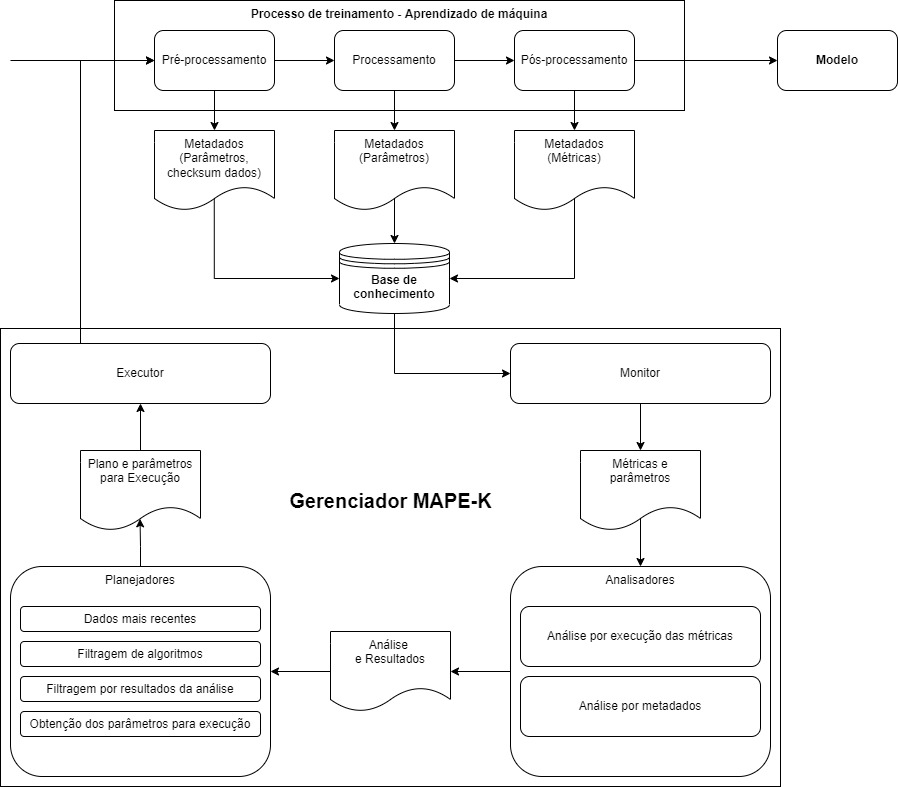
\includegraphics[scale=0.5]{images/ML-MAPE-K.jpg}
\caption {Adequação do workflow ao gerenciador MAPE-K}
\label{fig:MLMAPEK}
\end{figure}

Após a obtenção de tal Base de Conhecimento, e possível verificar como as etapas de cada parte do MAPE-K serão desenvolvidas. Conforme ilustrado na Figura \ref{fig:MLMAPEK}, as etapas de Análise e Planejamento foram subdivididas em diferentes estratégias para o MAPE-K ser configurável durante o processo de escolha, enquanto as etapas de monitoria e execução foram configuradas com uma única estratégia. As estratégias das etapas de Análise e Planejamento podem ser ativadas ou desativadas conforme o que é definido como \textit{Feature Toggles}~\citep{Rahman_2016}~\citep{Mahdavi-hezaveh_2021}, por meio de arquivos JSON presentes no projeto conforme ilustrado no Trecho \ref{cod:FeatureToggle}.

\begin{lstlisting}[language=Python, caption=Exemplo de arquivo utilizando \textit{Feature Toggles},label=cod:FeatureToggle]
{
	"ml_algorithm_validation": true,
	"ml_data_checksum": false,
	"ml_pipeline": false,
	"ml_pipeline_threshold": true	
}
\end{lstlisting}

\subsubsection{Monitoria}

Para a etapa de monitoria, os dados são obtidos em cada arquivo presente na base de conhecimento e separados em dois conjuntos diferentes: Um contendo os metadados e informações relativas a execução do \textit{Workflow} (checksum do conjunto de dados, estatísticas e parâmetros de execução do \textit{Workflow}) e outro contendo as métricas obtidas pelo modelo resultante dessa execução, ambos possuindo um identificador do arquivo para estabelecer consistência entre os dados dos dois conjuntos. Os arquivos podem ser filtrados pelo conjunto de dados e pelo atributo protegido, ou não possuir filtro obtendo todos os dados possíveis.

\subsubsection{Análise}

Para a etapa de análise, é realizado um cálculo de pesos baseado em uma seleção livre das métricas. O motivo de existir esse cálculo é mensurar o contexto do problema de acordo com uma análise prévia do Cientista de Dados e do Especialista de Domínio, e consolidar todas as métricas para simplificar as estratégias de planejamento. É possível encontrar abordagens similares e com objetivos similares, porém em diferentes contextos, pesquisando em artigos acadêmicos~\citep{Konstantinou_2017}.

\begin{lstlisting}[language=Python, caption={Exemplo de arquivo contendo informações sobre as métricas, grupos e seus respectivos pesos},label=cod:MetricsWeights]
{
  "metrics_groups": [
    {
      "group_name": "standard",
      "weight": 0.5,
      "metrics": {
        "accuracy": {
          "weight": 0.5,
          "normalize": null
        },
        "f1_score": {
          "weight": 0.5,
          "normalize": null
        }
      }
    },
    {
      "group_name": "fairness",
      "weight": 0.5,
      "metrics": {
        "statistical_parity_difference": {
          "weight": 0.33,
          "normalize": "diff"
        },
        "equal_opportunity_difference": {
          "weight": 0.33,
          "normalize": "diff"
        },
        "average_abs_odds_difference": {
          "weight": 0.34,
          "normalize": "diff"
        }
      }
    }
  ]
}
\end{lstlisting}

As métricas são divididas em dois grupos (Métricas de performance e Metricas de Fairness), e dentro desse grupo pode-se colocar quantas métricas forem necessárias, desde que seja respeitado o contexto de cada grupo. A cada grupo é atribuído pesos diferentes, e a cada métrica desse grupo também é atribuído pesos diferentes, conforme ilustrado no Trecho \ref{cod:MetricsWeights}. Primeiro, normaliza-se as métricas $m_{F_i}$ para $m'_{F_i}$, referentes às métricas de Fairness, para todas ficarem em um intervalo de 0 a 1, conforme exibido na equação \ref{eqn:normalizationFairness}. Dessa forma, seus resultados ficam uniformes e é possível aplicar os pesos sem haver distorções no cálculo. No caso das métricas de Performance, todas possuem a mesma escala, por isso as métricas $m_{P_i}$ não são normalizadas. Depois, multiplica-se cada uma por seus pesos correspondentes $w_{P_i}$ e $w_{F_i}$, e realiza-se uma média ponderada dentro do grupo para atribuir uma pontuação $S_P$ para o grupo das Métricas de Performance e $S_F$ para o grupo das Metricas de Fairness, conforme exibido na equação \ref{eqn:groupScores}. Para facilitar a visualização das pontuações, multiplica-se as pontuações por um fator $X = 1000$ para o intervalo da pontuação ser de 0 a 1000 e arredonda-se o número. Após tais pontuações serem obtidas, a pontuação geral $S$ é calculada multiplicando-as por seus pesos correspondentes $w_P$ e $w_F$ e realizando a média ponderada, conforme exibido na equação \ref{eqn:totalScore}.

\begin{equation}
\label{eqn:normalizationFairness}
	\begin{aligned}
	m'_{F_i} = 
	\begin{cases}
	1-\lvert m_{F_i} \rvert & \text{caso $m_{F_i}$ envolva diferen\c{c}a e $-1 < m_{F_i} < 1$}\\
	0 & \text{caso $m_{F_i}$ envolva diferen\c{c}a, e $m_{F_i} >= 1$ ou $m_{F_i} <= -1$}\\
	1-\lvert \frac{1}{m_{F_i}}-1 \lvert & \text{caso $m_{F_i}$ envolva razão e $m_{F_i} > 1$}\\
	1-\lvert m_{F_i}-1 \lvert & \text{caso $m_{F_i}$ envolva razão e $m_{F_i} <= 1$}\\
	m_{F_i} & \text{caso contrário}
	\end{cases}
	\end{aligned}
\end{equation}

\begin{equation}
\label{eqn:groupScores}
	\begin{aligned}
	S_F = \round*{X \times \frac{\sum_{i=1}^{n_F} w_{m'_{F_i}} \times m'_{F_i}}{\sum_{i=1}^{n} w_{m'_{F_i}}}}\\
	S_P = \round*{X \times \frac{\sum_{i=1}^{n_P} w_{m_{P_i}} \times m_{P_i}}{\sum_{i=1}^{n} w_{m_{P_i}}}}
	\end{aligned}
\end{equation}

\begin{equation}
\label{eqn:totalScore}
	S = \frac{w_F \times S_F + w_P \times S_P}{w_F + w_P}
\end{equation}

Nesta etapa, foram desenvolvidas as seguintes estratégias, cujos motivos para existir e funcionamento estão explicados abaixo:

\begin{itemize}
\item \textbf{Análise por execução das métricas:} É atribuída a cada execução presente no conjunto uma pontuação conforme o cálculo explicado acima, e as pontuações são passadas adiante para a fase de planejamento.
\item \textbf{Análise por metadados:} Para o desenvolvimento de melhores estratégias de planejamento, alguns metadados, como data de execução, são analisados e o conjunto resultante é enriquecido com esses metadados mais específicos.
\end{itemize}

\subsubsection{Planejamento}

Para a etapa de planejamento, foram desenvolvidas as seguintes estratégias, cujos motivos para existir e funcionamento estão explicados abaixo, para a escolha dos melhores modelos:

\begin{itemize}
\item \textbf{Dados mais recentes:} Os dados podem ser modificados de acordo com a execução e a qualidade das métricas são melhor definidas de acordo com a qualidade dos dados. Nesta estratégia, é realizado um filtro baseado na assinatura do dado com a execução mais recente, que só é possível de ser obtida se a análise dos metadados for executada.
\item \textbf{Filtragem de algoritmos:} Alguns algoritmos podem estar mal implementados ou seus modelos podem estar com métricas que necessitam uma melhor análise do Cientista de Dados para serem consideradas confiáveis. Para isso não acontecer, é possível realizar um filtro de acordo com as combinações de algoritmos consideradas confiáveis antes de selecionar os modelos ideais.
\item \textbf{Fase por resultados da análise:} Pelo mesmo motivo da estratégia anterior, métricas não confiáveis significam uma distorção na pontuação final. Para esse caso, foi criado um limiar de pontuação mínimo e máximo para determinar pontuações que podem ser consideradas confiáveis para avaliação.
\item \textbf{Obtenção dos parâmetros para execução:} Alguns dos modelos restantes são selecionados de acordo com as maiores pontuações e os parâmetros presentes nestes modelos selecionados são obtidos.
\end{itemize}

Após a execução das mesmas, caso estejam ativadas, os parâmetros selecionados são passados para a etapa de execução.

\subsubsection{Execução}

Para a etapa de execução, os parâmetros selecionados na fase de planejamento são configurados como parâmetros para a execução do \textit{Workflow}, e esta execução pode ampliar a Base de Conhecimento ou não dependendo do valor da opção de gravação dos resultados.

\subsection{Interface Humano-Computador}

Durante o desenvolvimento do \textit{Workflow} e de seu componente autônomo, foi notado que o número de configurações e a complexidade das mesmas era muito grande, ocasionando problemas na hora de documentar e detalhar todo o processo executado. Para facilitar tais configurações, foi criada uma Interface Humano-Computador onde é condensada toda a organização das configurações e dos arquivos utilizados para a execução simples e autônoma do \textit{Workflow}, alem da própria realização destas execuções. Também foi criado um Backend para fazer a intermediação entre o Gerenciador Autonômico e a interface.

O Backend foi desenvolvido em Python para reusar códigos já desenvolvido em etapas anteriores, usando o framework Flask para construir as requisições web e foi dividido em 3 camadas. A camada \textit{web} corresponde às requisições que constroem a ponte entre Frontend e Backend, a camada \textit{service} corresponde às funcionalidades e casos de uso que serão chamados pelas requisições, e a camada \textit{repo} corresponde às operações de leitura e escrita que serão realizadas nos arquivos do \textit{Workflow}.

A interface foi desenvolvida em JavaScript devido a facilidade e a robustez para construir interfaces com a linguagem e ao acervo grande de ferramentas para facilitar o desenvolvimento, usando as bibliotecas React e Redux e a biblioteca de componentes Material UI para economizar tempo com componentes já prontos, uma vez que o foco deste trabalho não exige componentes específicos para a interface. O uso da Material UI permite um \textit{look-and-feel} similar a aplicativos desenvolvidos para o Sistema Operacional para dispositivos móveis Android, uma vez que é baseado nas \textit{guidelines} do Material Design elaborados pelo Google.

A interface foi nomeada de FairPEK, junção dos termos Fairness e MAPE-K, e possui os seguintes detalhes:

\subsubsection{Opções do Menu}

Conforme ilustrado na Figura \ref{fig:opcoesMenu}, o menu pode ser expandido e recolhido, onde suas opções são selecionáveis independente da configuração, e foram colocados ícones ao lado do nome de sua opção para que a localização das opções seja acessível mesmo com o menu recolhido.

\begin{figure}[H]
    \centering
    \subfigure[fig:opcoesMenu1][Opções de seleção de menu expandidas.]{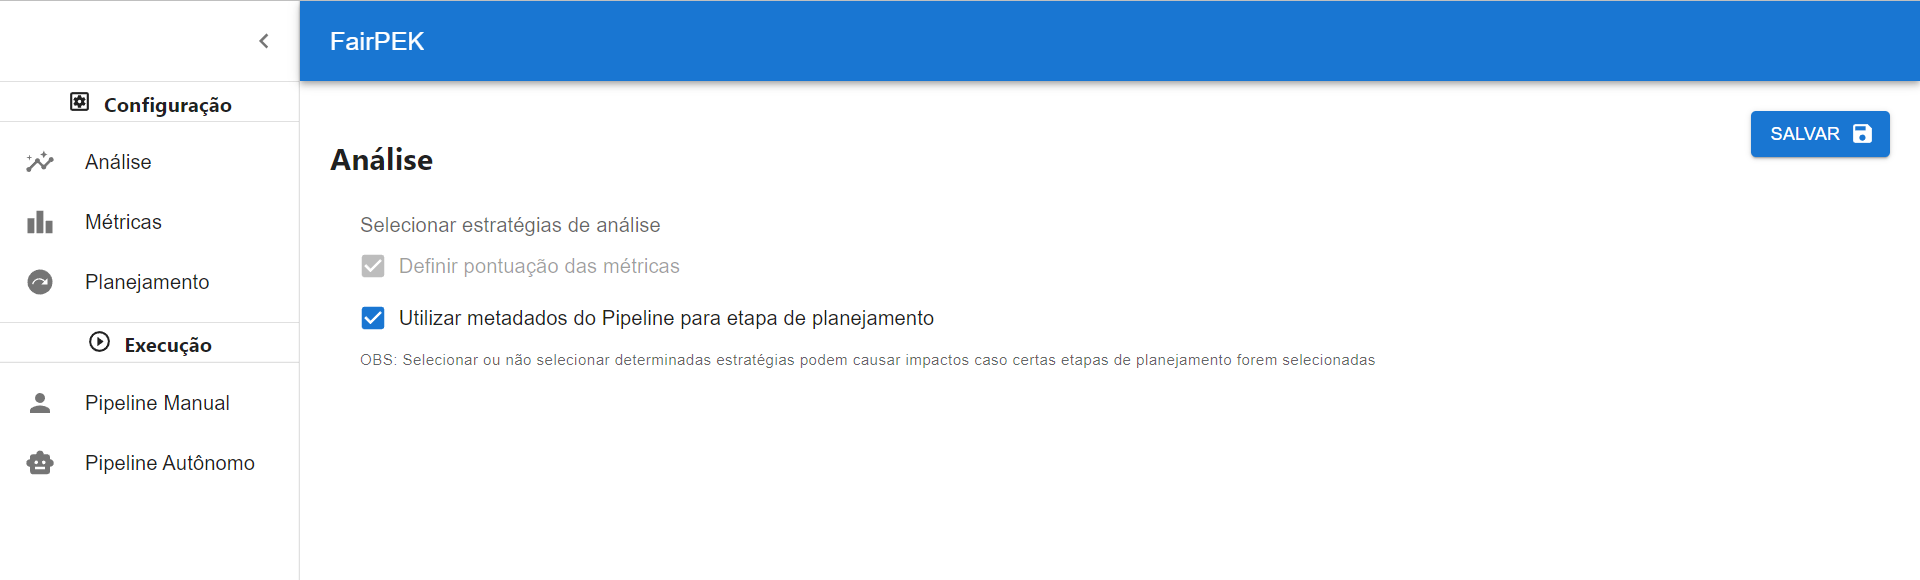
\includegraphics[scale=0.4]{images/front/Menu.png}}
    \subfigure[fig:opcoesMenu2][Opções de seleção de menu recolhidas.]{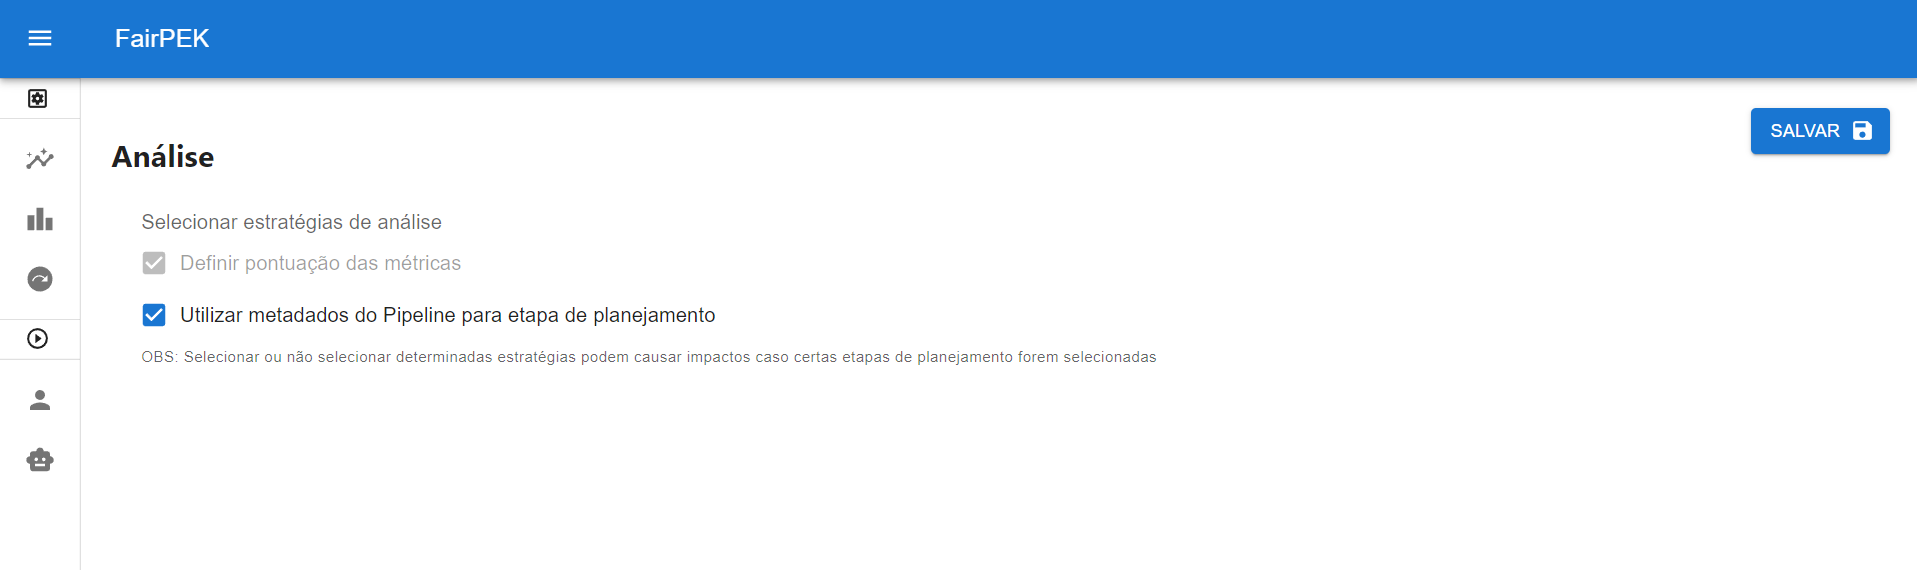
\includegraphics[scale=0.4]{images/front/Analise.png}}
    \caption{Comportamento das opções de menu.}
    \label{fig:opcoesMenu}
\end{figure}

No menu, as opções são divididas em Configuração e Execução. Em Configuração, há as opções Análise, Métricas e Planejamento relativas às configurações presentes no Gerenciador Autonômico. Em Execução, há as opções Pipeline Manual e Pipeline Autônomo relativas às maneiras de como realizar uma execução do \textit{Workflow}.

\subsubsection{Configurações para Análise}

Ao clicar a opção do menu "Análise", é exibida a tela ilustrada na Figura \ref{fig:configAnalise}. Ela possui apenas duas opções, relativas às estratégias desenvolvidas na parte de análise do Gerenciador Autonômico. Ao clicar no botão "Salvar" localizado no canto superior direito, é chamada uma requisição que salva o arquivo com as opções selecionadas e é exibida uma indicação de sucesso no canto inferior esquerdo.

\begin{figure}[H]
    \centering
    \subfigure[fig:configAnalise1][Opções para configurar etapa de análise.]{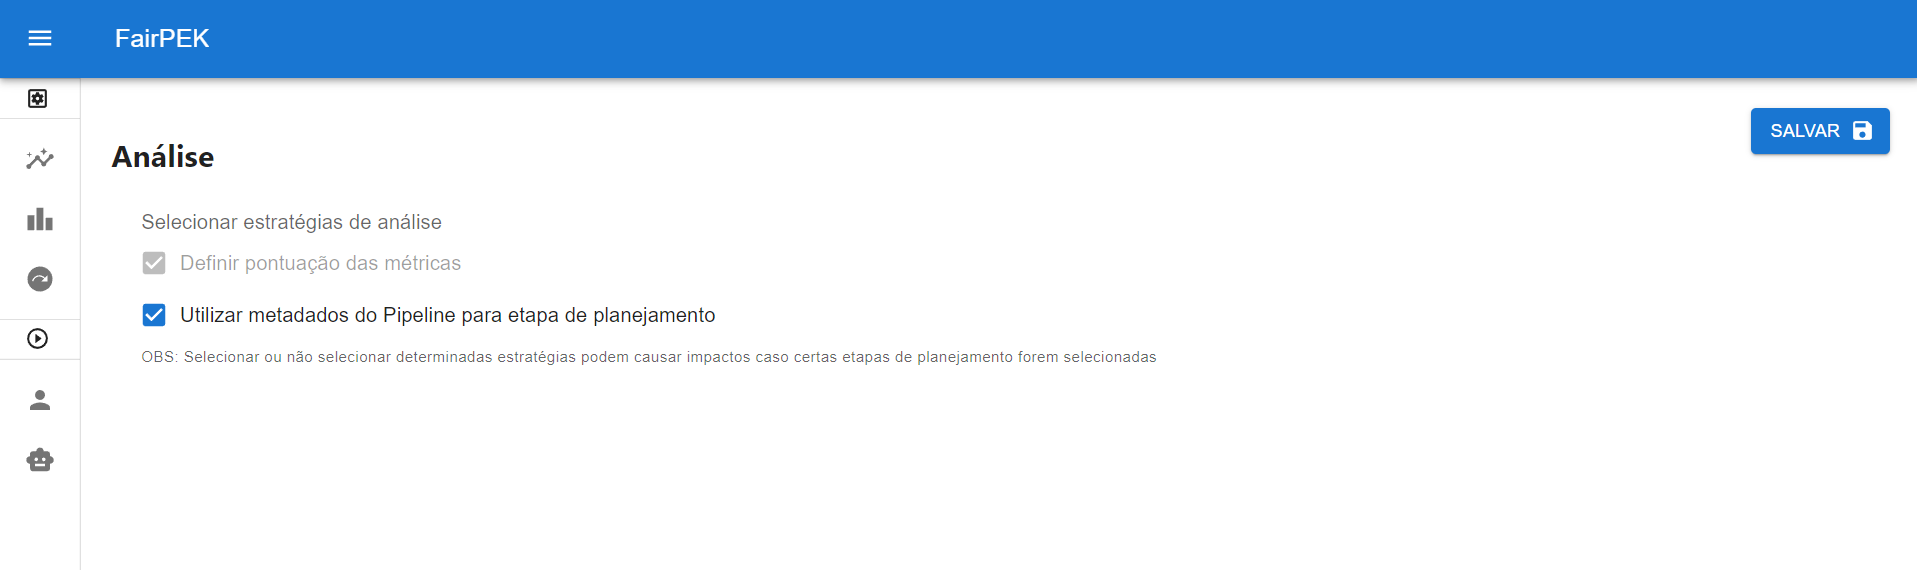
\includegraphics[scale=0.4]{images/front/Analise.png}}
    \subfigure[fig:configAnalise2][Indicação de sucesso da operação.]{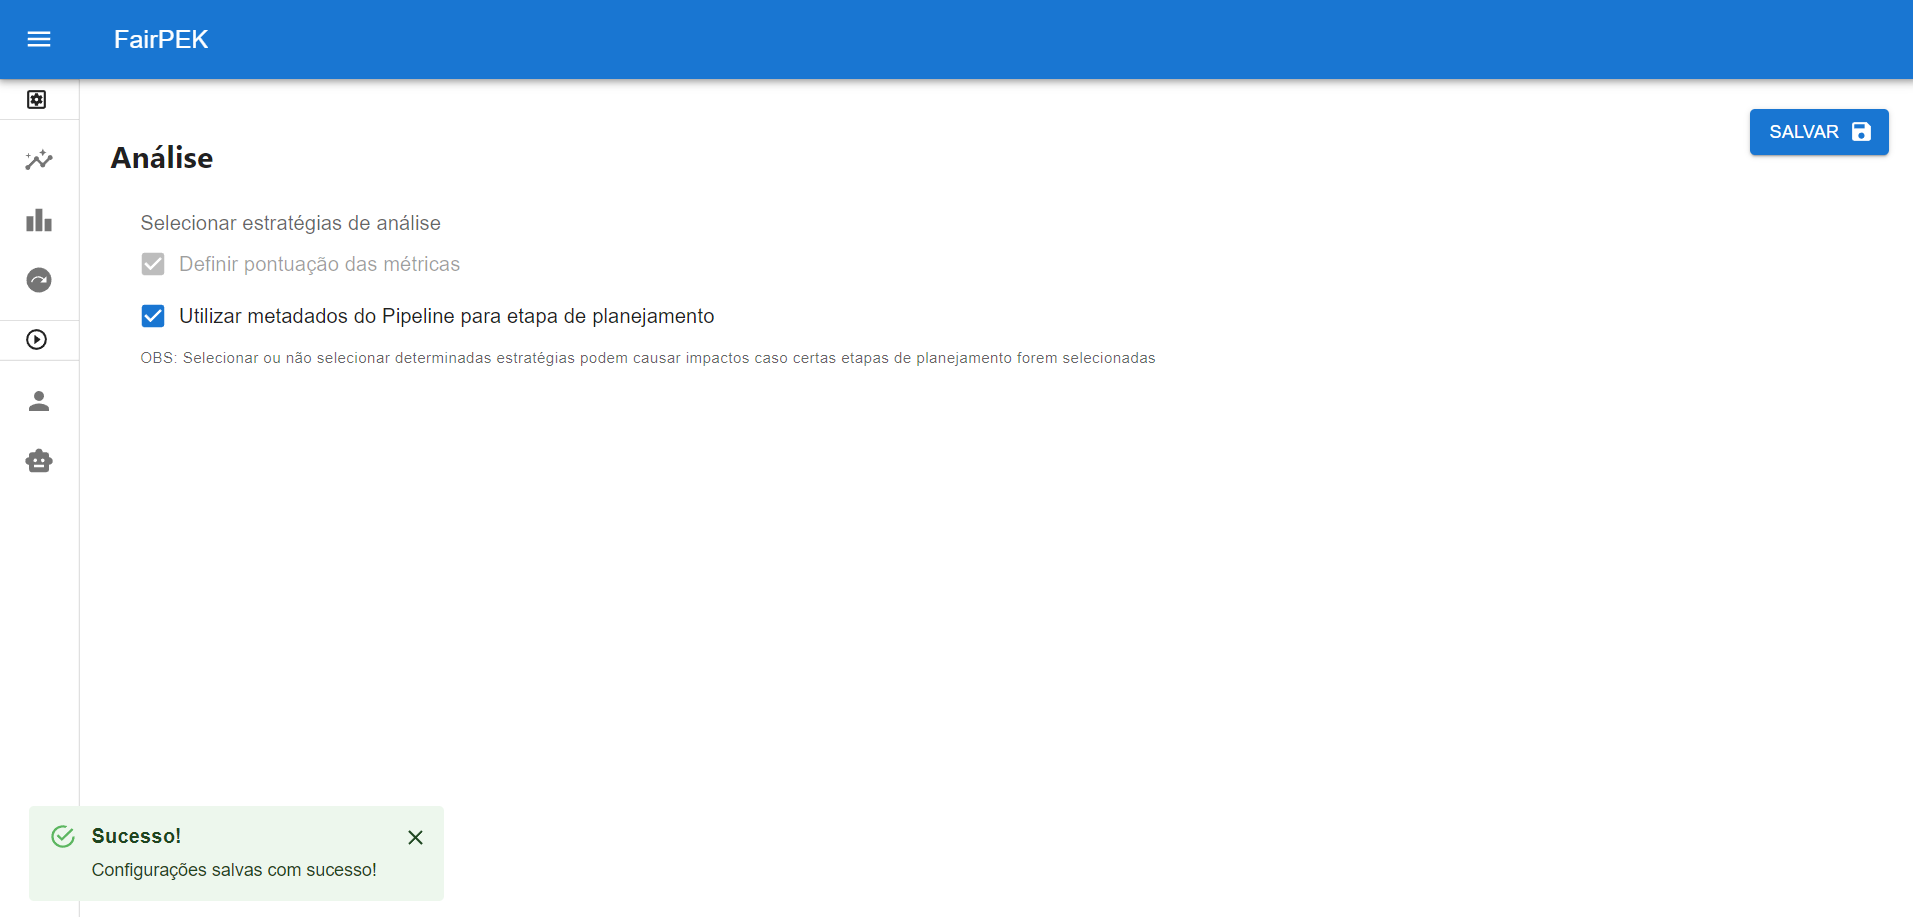
\includegraphics[scale=0.4]{images/front/Analise-Sucesso.png}}
    \caption{Configuração da etapa de análise para o workflow autônomo.}
    \label{fig:configAnalise}
\end{figure}

Uma das duas estratégias está desabilitada pois foi desenvolvida como a estratégia padrão usada pelo Gerenciador Autonômico. Se a estratégia de utilizar metadados não for habilitada, certas opções marcadas na etapa de planejamento podem não funcionar.

\subsubsection{Configurações das Métricas}

Ao clicar a opção do menu "Métricas", é exibida a tela ilustrada na Figura \ref{fig:configMetricas}. Ela é dividida em duas abas: Métricas de Avaliação e Métricas de Fairness, relativas aos grupos de métricas divididos no Gerenciador Autonômico. Em ambas as abas, há os campos de peso para avaliação, que simboliza o peso no cálculo da pontuação final, e o campo de métricas para uso, que determina quais métricas serão utilizadas para o calculo da pontuação de cada grupo. Uma vez que há apenas duas abas, a alteração do campo de peso para avaliação de uma aba automaticamente alterará o campo de peso para avaliação da outra aba para complementar a soma de 100\% sem precisar de validações.

\begin{figure}[H]
    \centering
    \subfigure[fig:configMetricas1][Configuração para Métricas de Performance.]{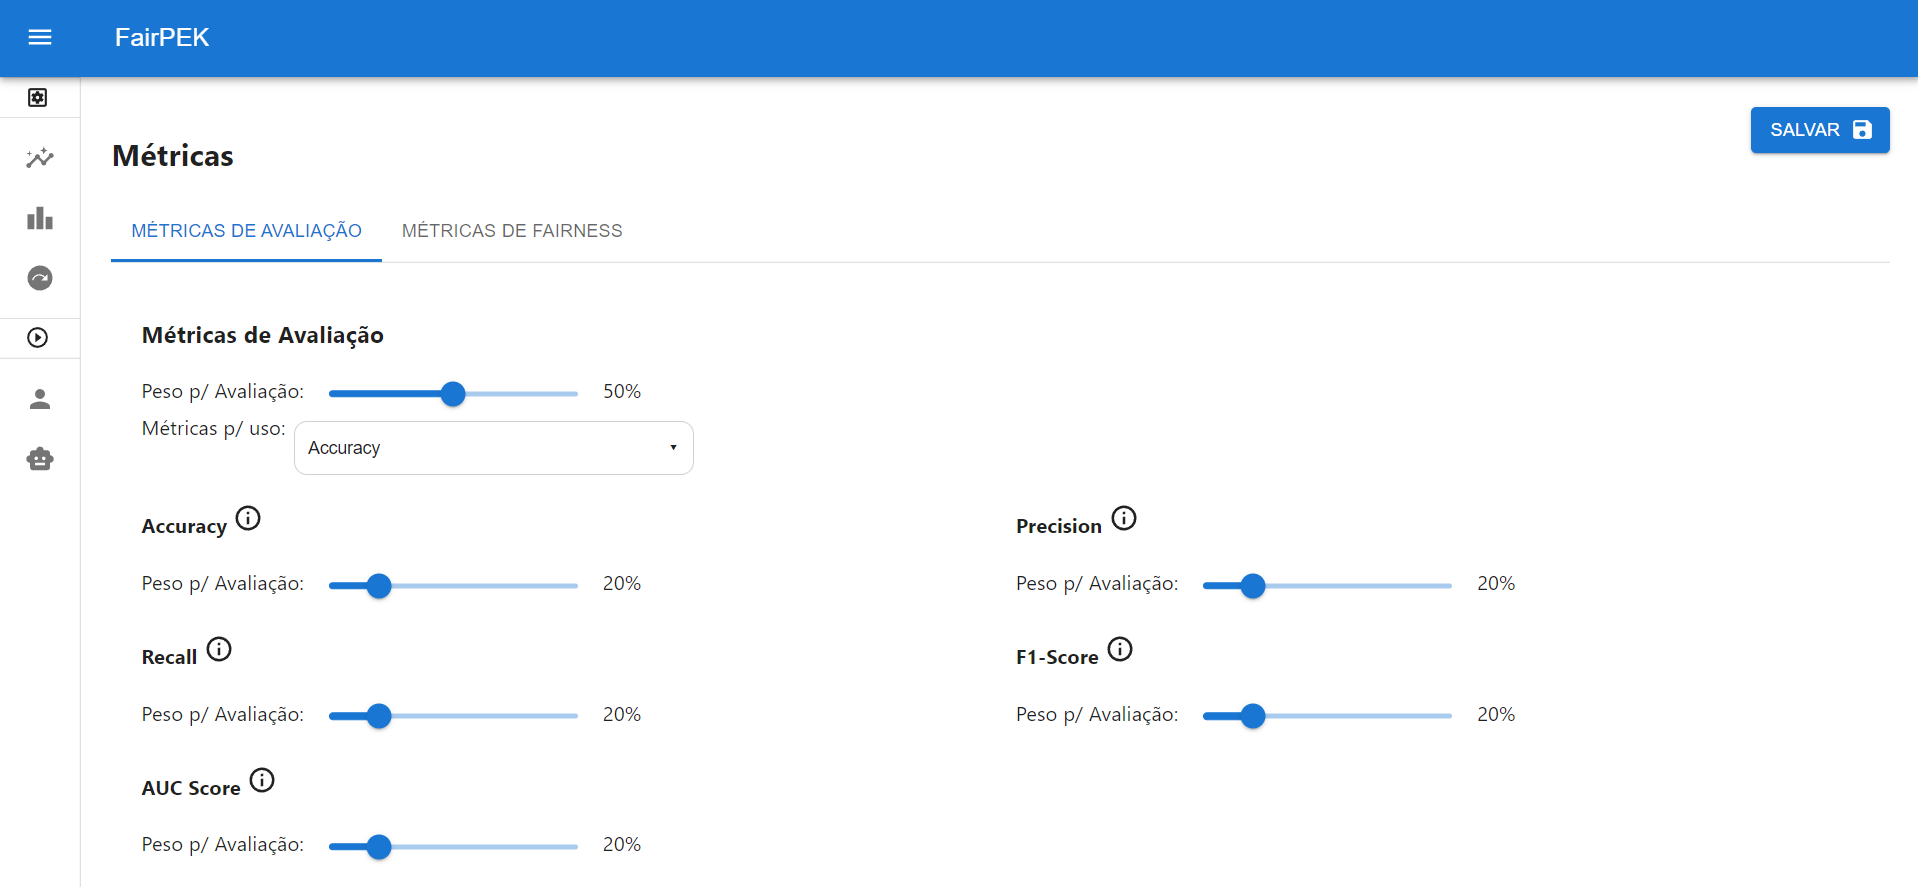
\includegraphics[scale=0.4]{images/front/Metricas-Performance.png}}
    \subfigure[fig:configMetricas2][Configuração para Métricas de Fairness.]{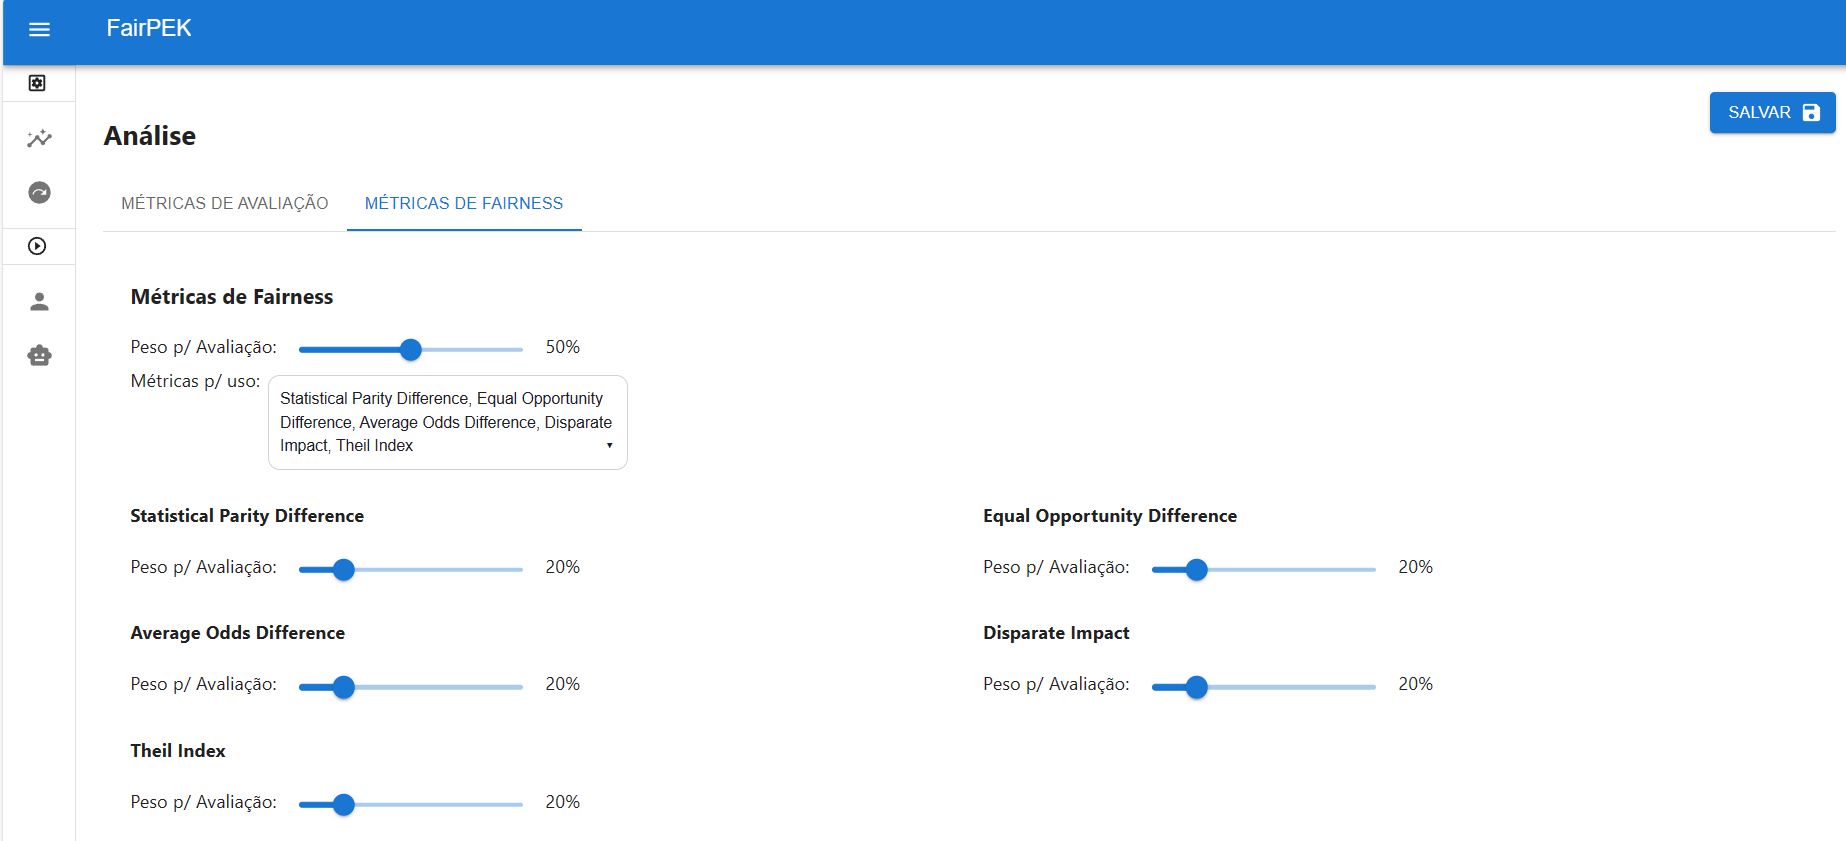
\includegraphics[scale=0.4]{images/front/Metricas-Fairness.png}}
    \caption{Configuração das métricas para etapa de análise do workflow autônomo.}
    \label{fig:configMetricas}
\end{figure}

A alteração do campo de métricas para uso implicará na presença de mais ou menos métricas para alterar os pesos para o cálculo da pontuação para o grupo de métricas. Uma vez que eu posso ter mais de duas métricas nesse caso, cpmplementar a soma de todas as métricas automaticamente para 100\% seria uma tarefa com maior complexidade, e por isso foi substituída por uma validação, conforme ilustrado na Figura \ref{fig:cenariosMetricas}. Ao clicar no botão "Salvar" localizado no canto superior direito, é realizada a validação da soma de todas as métricas e, em caso positivo, chamada uma requisição que salva o arquivo com as opções selecionadas e seus respectivos valores. Após este procedimento, será exibida uma indicação de sucesso ou erro de validação no canto inferior esquerdo indicando se o arquivo foi salvo ou não.

\begin{figure}[H]
    \centering
    \subfigure[fig:cenariosMetricas1][Erros de validação ao concluir a operação.]{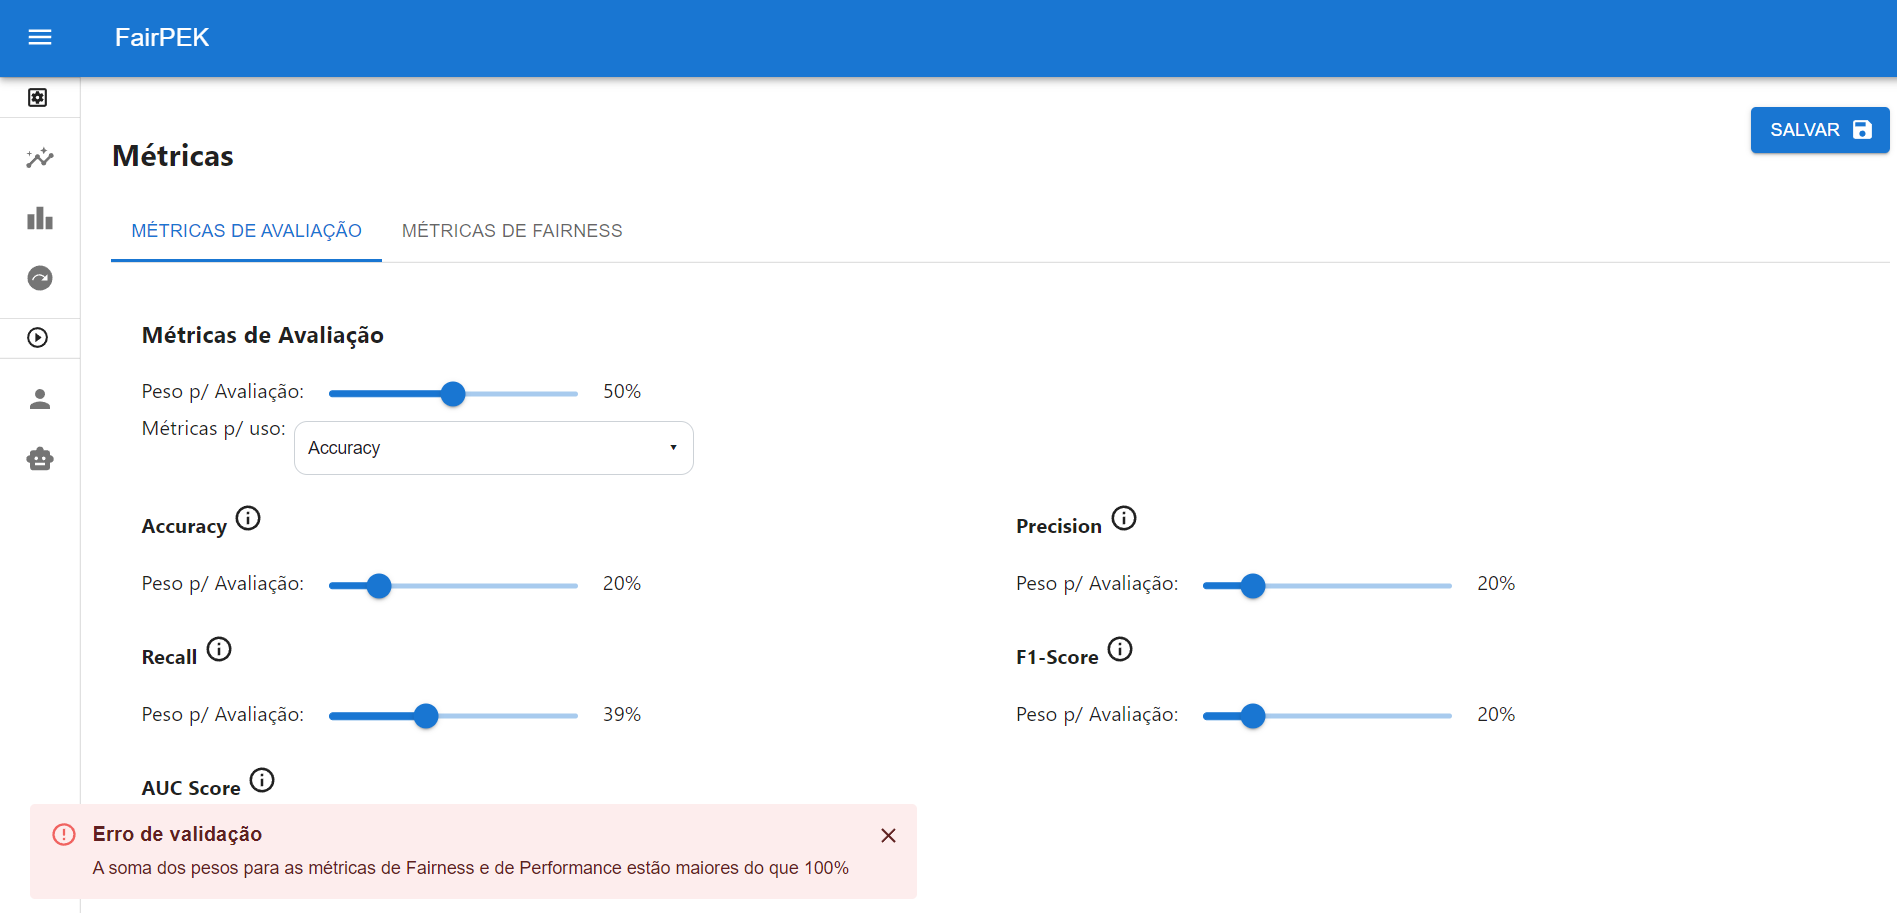
\includegraphics[scale=0.4]{images/front/Metricas-Erro.png}}
    \subfigure[fig:cenariosMetricas2][Indicação de sucesso da operação.]{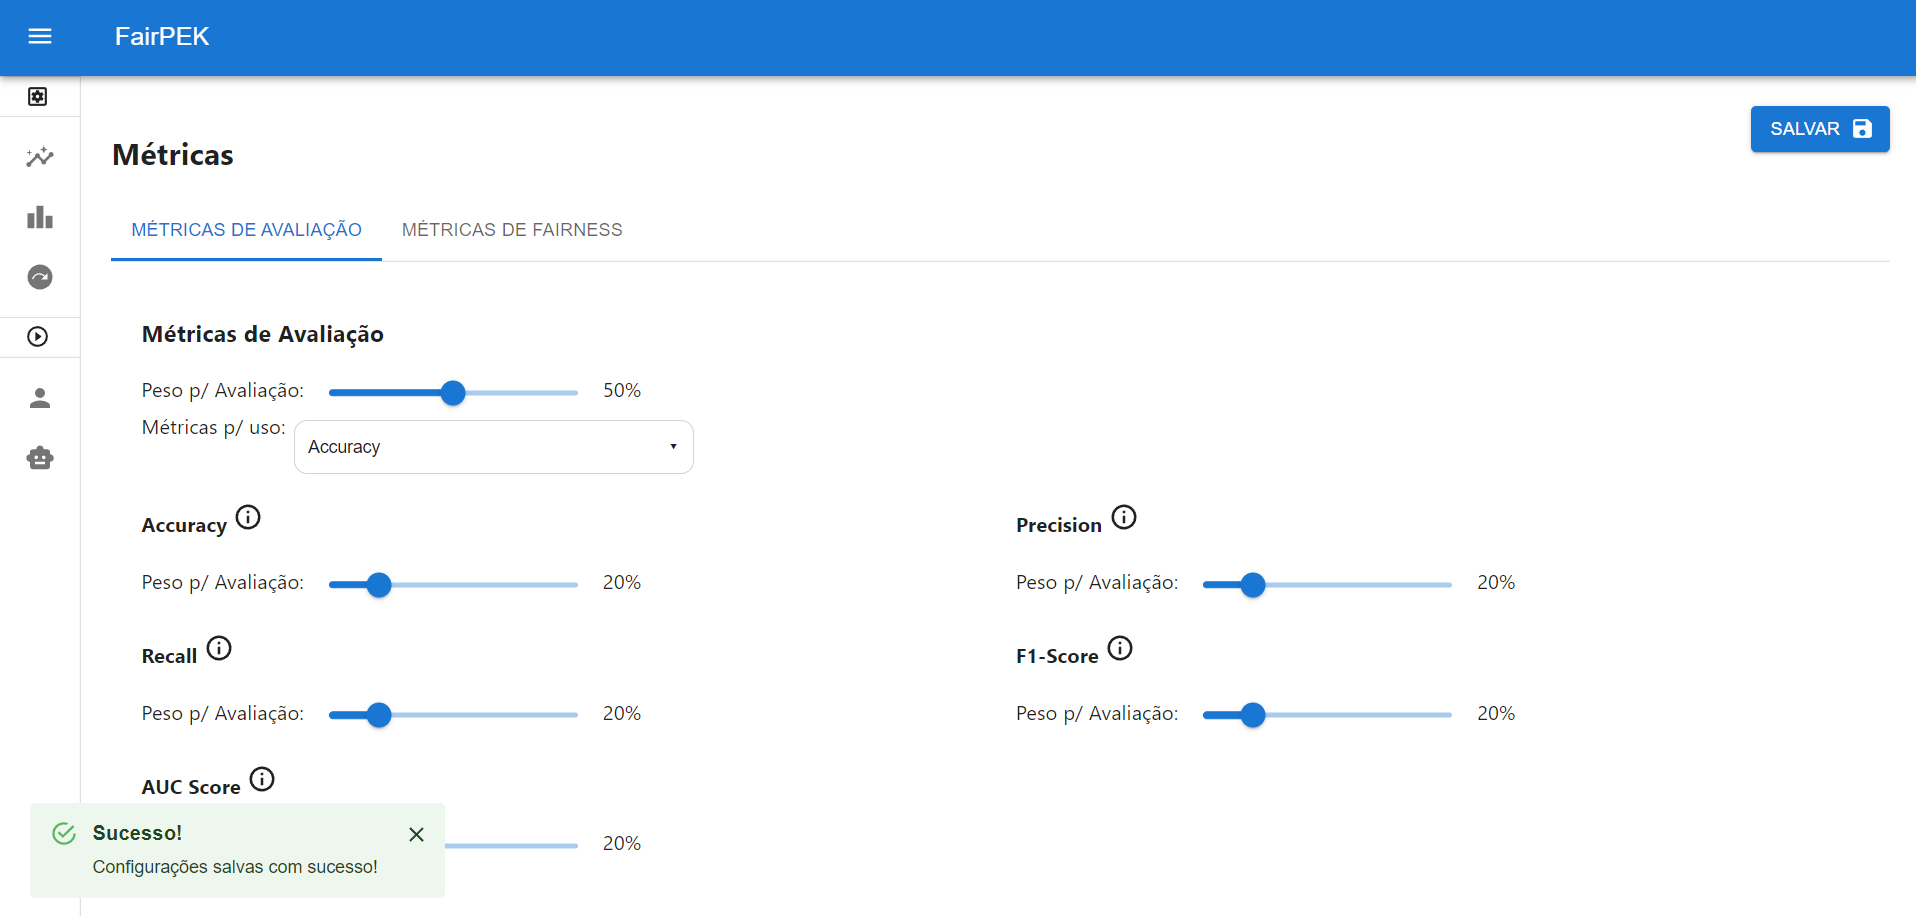
\includegraphics[scale=0.4]{images/front/Metricas-Sucesso.png}}
    \caption{Cenários possíveis na configuração das métricas.}
    \label{fig:cenariosMetricas}
\end{figure}

\subsubsection{Configurações para Planejamento}

Ao clicar a opção do menu "Planejamento", é exibida a tela ilustrada na Figura \ref{fig:configPlanejamento}. Ela possui quatro opções, relativas às estratégias desenvolvidas na parte de análise do Gerenciador Autonômico. Ao clicar no botão "Salvar" localizado no canto superior direito, são chamadas requisições que salvam os arquivos necessários e é exibida uma indicação de sucesso no canto inferior esquerdo.

\begin{figure}[H]
    \centering
    \subfigure[fig:configPlanejamento1][Opções para configurar etapa de planejamento.]{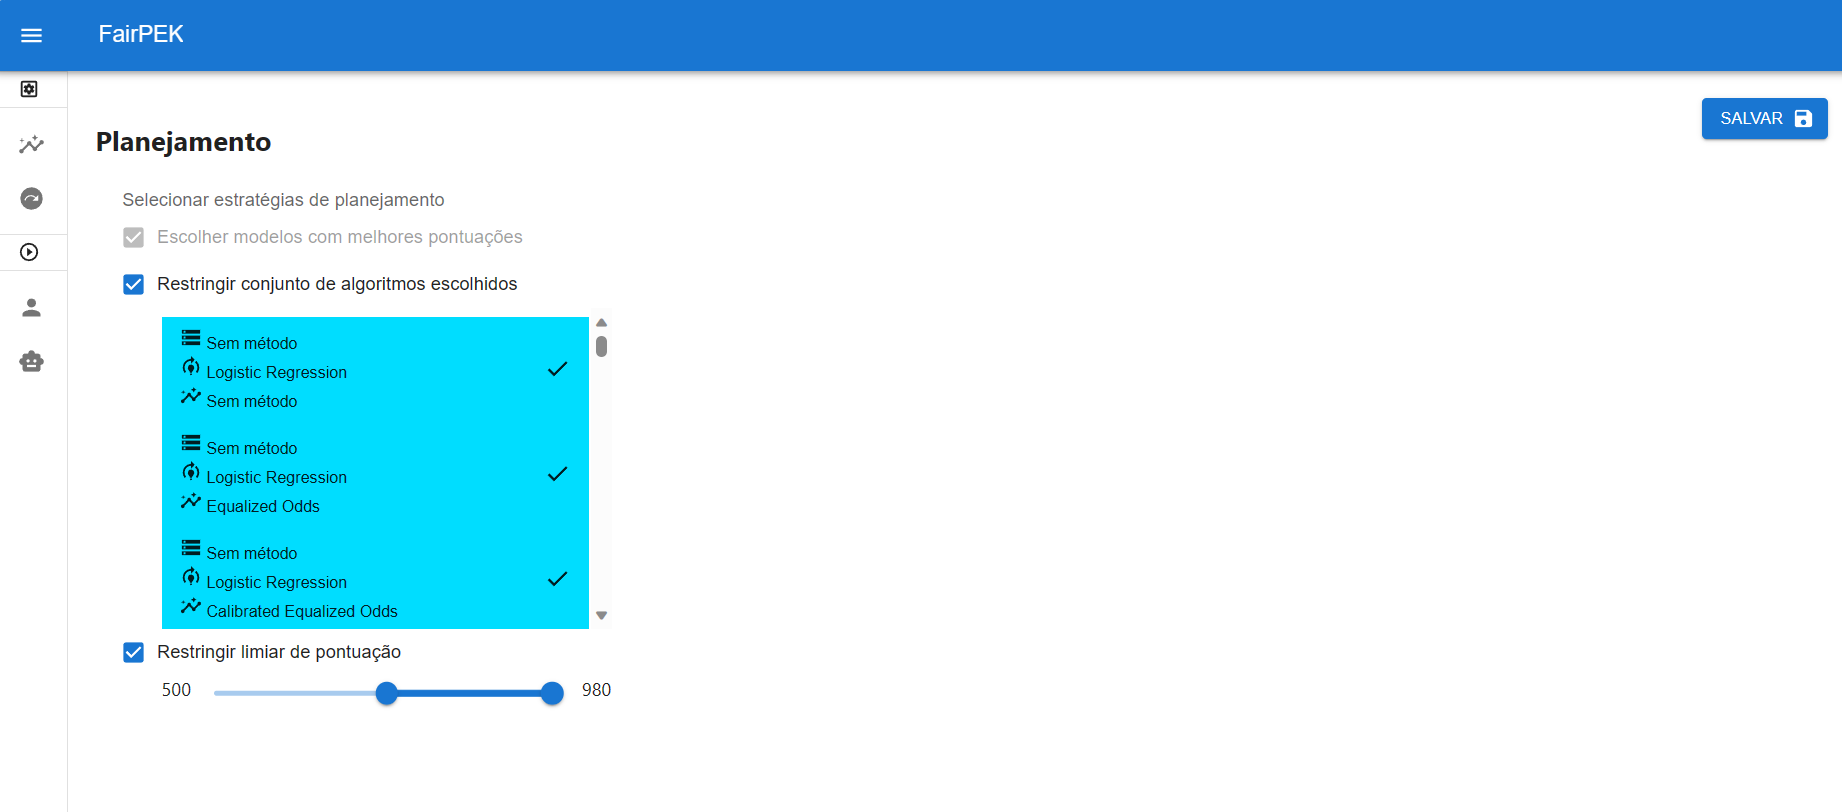
\includegraphics[scale=0.4]{images/front/Planejamento.png}}
    \subfigure[fig:configPlanejamento2][Indicação de sucesso da operação.]{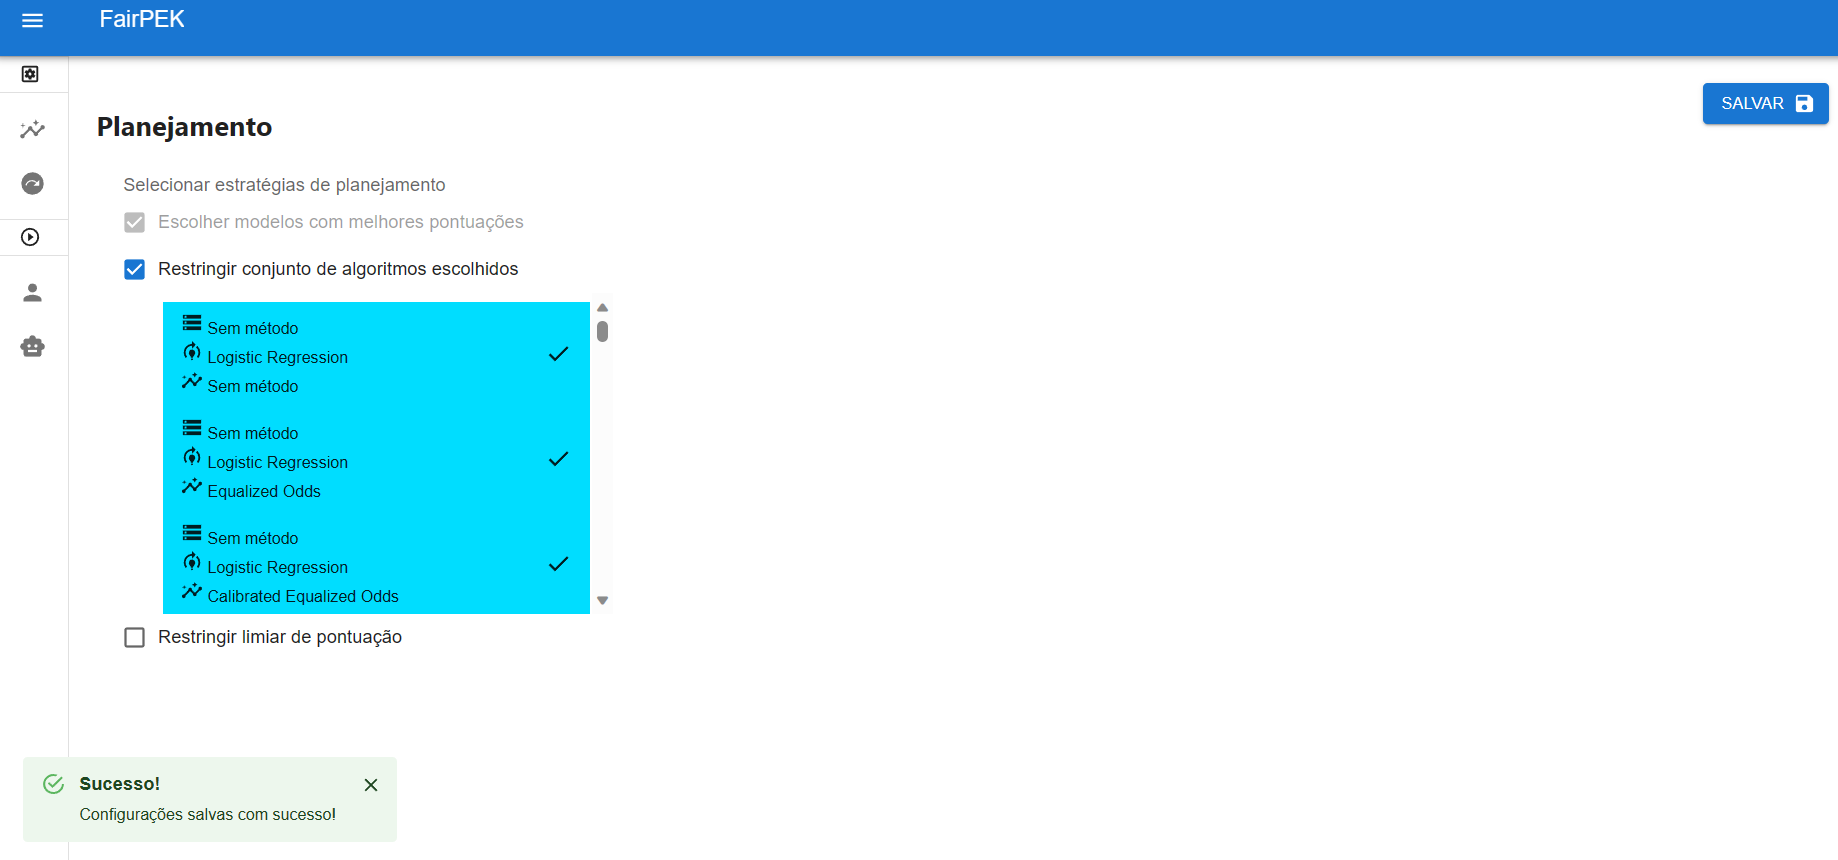
\includegraphics[scale=0.4]{images/front/Planejamento-Sucesso.png}}
    \caption{Configuração da etapa de planejamento para o workflow autônomo.}
    \label{fig:configPlanejamento}
\end{figure}

Se a estratégia de restrição de algoritmos for selecionada, é exibido um submenu contendo as combinações de algoritmos que podem ser selecionadas que são salvas em um arquivo separado para serem filtrados na etapa de planejamento. Se a estratégia de restrição por um limiar de pontuação for selecionada, é exibido um slider com uma pontuação mínima e uma pontuação máxima, e ambas as pontuações são salvas em um arquivo separado para serem filtrados na etapa de planejamento.

\subsubsection{Execução simples do Workflow}

Ao clicar a opção do menu "Pipeline Manual", é exibida a tela ilustrada na Figura \ref{fig:pipelineManual}. Ela possui indicações de etapas divididas em Parametrização, Execução e Resultados, campos para selecionar o conjunto de dados e o atributo protegido e opções para selecionar onde a redução de viés será executada. Dependendo da opção selecionada, aparecem campos para selecionar o algoritmo de treinamento e o algoritmo de redução de viés. Ao clicar no botão "Executar" localizado no canto superior direito, é feita uma requisição para executar o \textit{Workflow} com as opções selecionadas, é exibida uma indicação de sucesso no canto inferior esquerdo e a indicação de etapa é atualizada para a etapa de execução.

\begin{figure}[H]
    \centering
    \subfigure[fig:pipelineManual1][Opções para executar o workflow manualmente.]{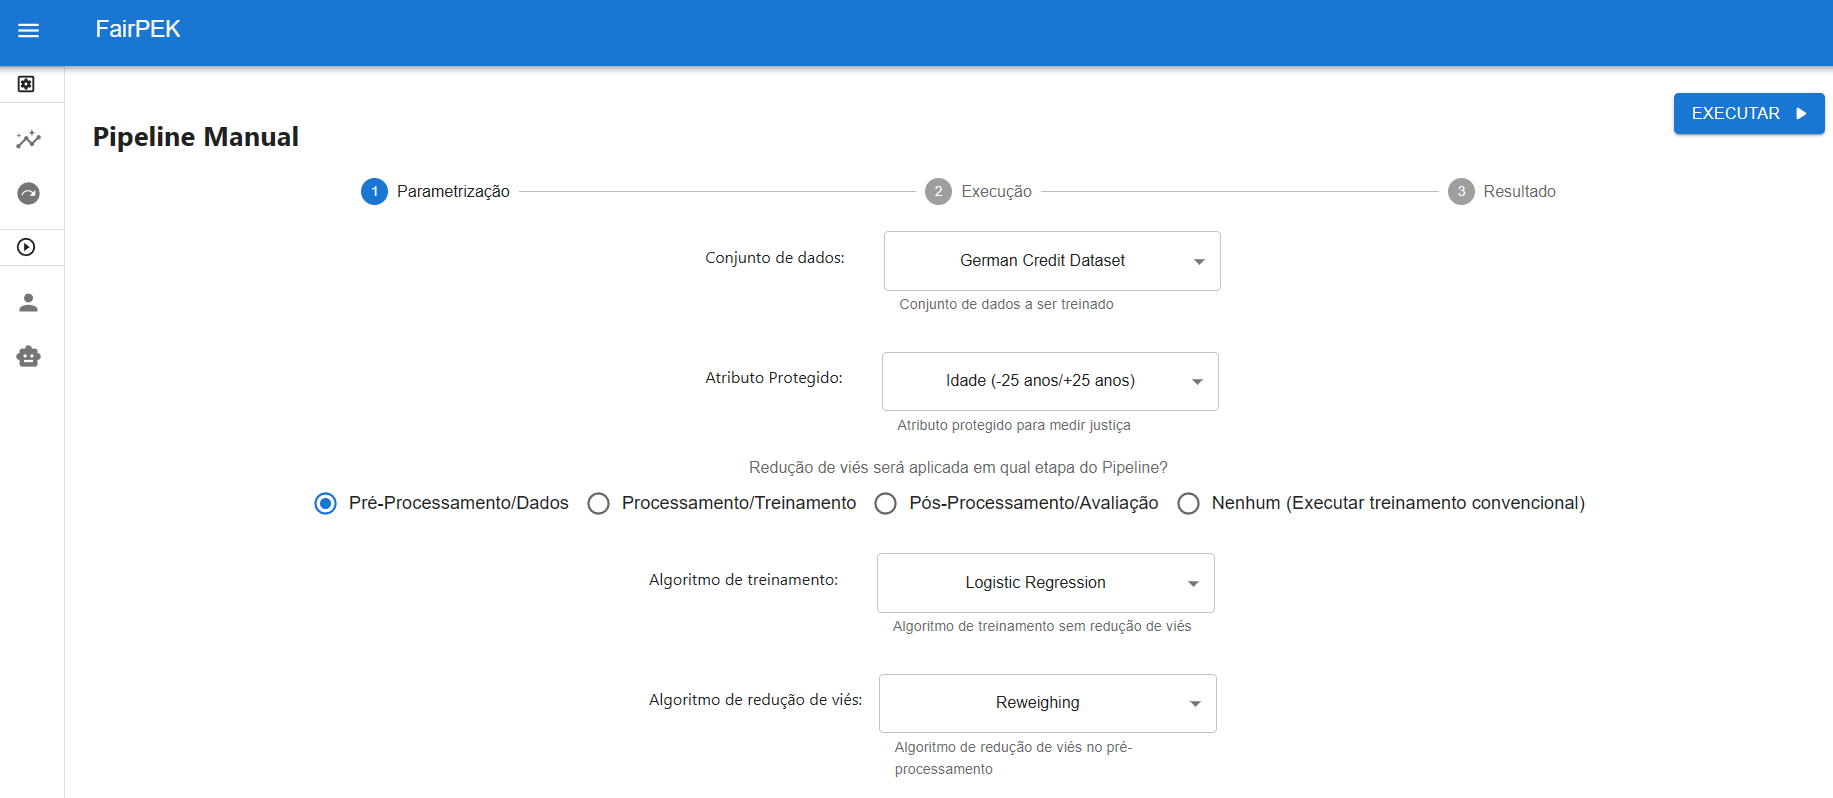
\includegraphics[scale=0.35]{images/front/Pipeline-Manual-Parametros.png}}
    \subfigure[fig:pipelineManual2][Workflow em execução.]{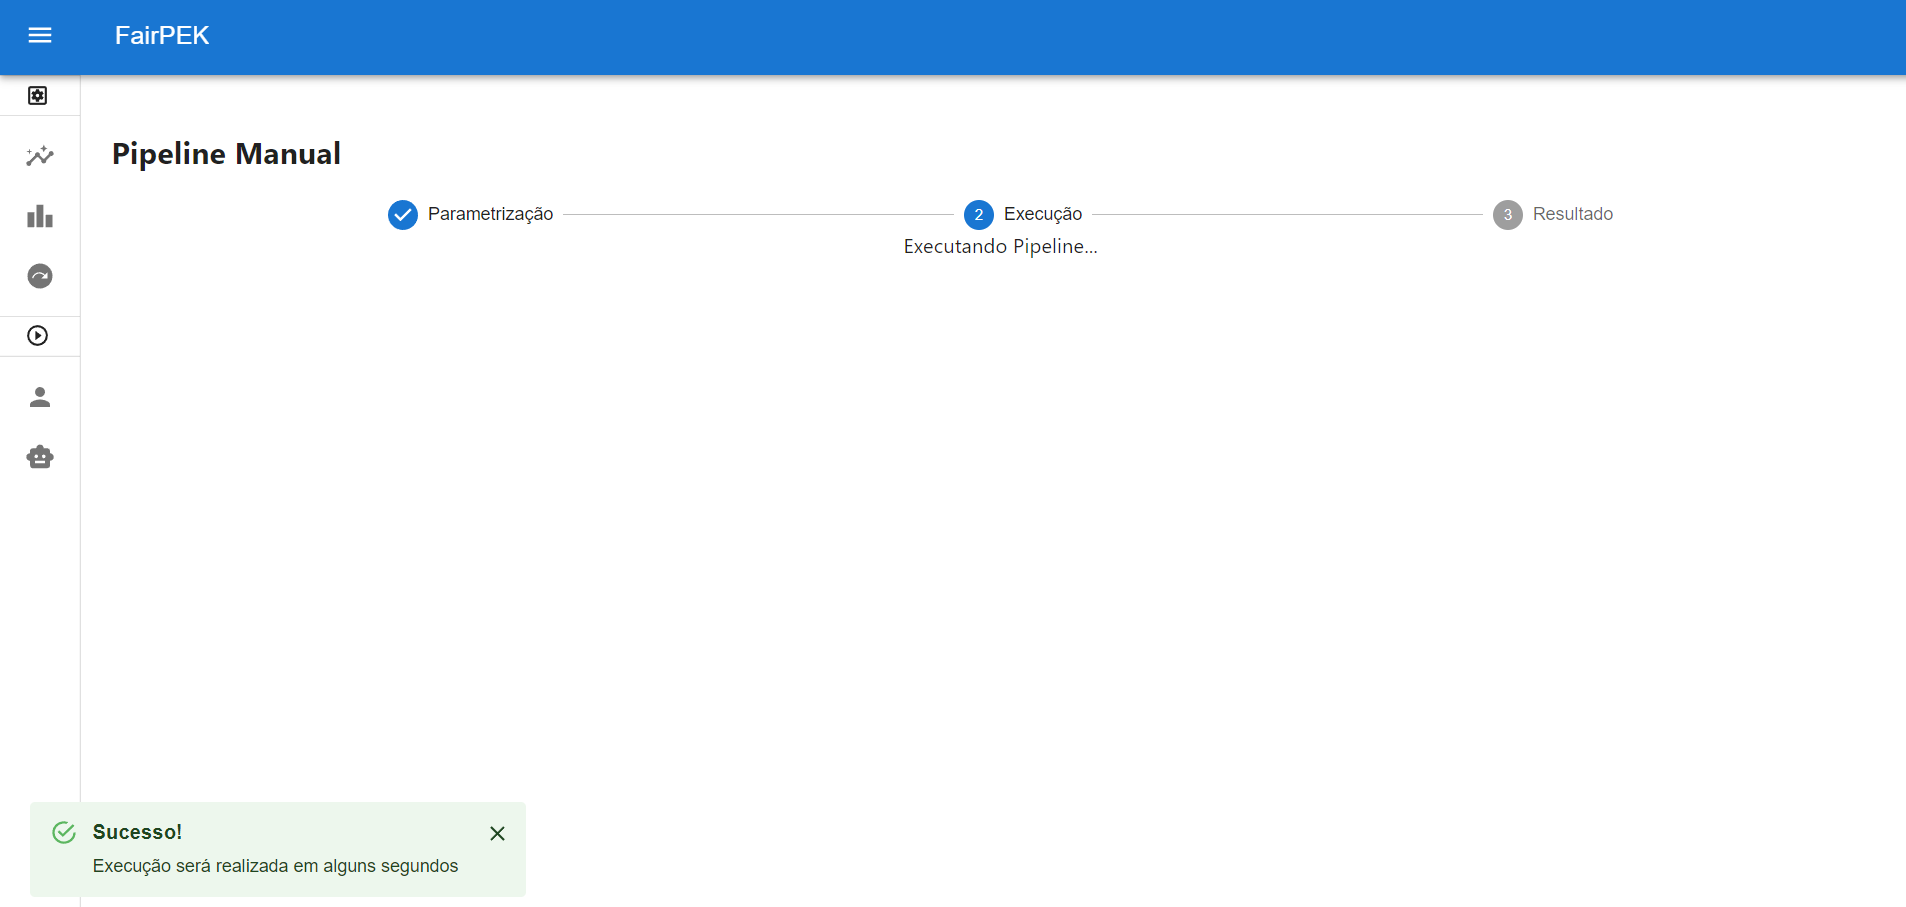
\includegraphics[scale=0.3575
    ]{images/front/Pipeline-Manual-Execucao.png}}
    \caption{Execução simples e manual do Workflow.}
    \label{fig:pipelineManual}
\end{figure}

Após a execução ser concluída,  a indicação de etapa é atualizada para a etapa de resultados, conforme ilustração nas Figuras \ref{fig:pipelineManualInfo} e \ref{fig:pipelineManualMetricas}. Nela, os parâmetros gravados são organizados em 4 grupos: Execução, relativos aos parâmetros utilizados e estatísticas da execução, Métricas de Performance, relativas aos resultados das métricas de Performance, Métricas de Fairness, relativas aos resultados das métricas de Fairness, e Pontuação, relativas ao cálculo realizado com as configurações utilizadas na parte de métricas.

\begin{figure}[H]
    \centering
    \subfigure[fig:pipelineManual1][Exibição dos parâmetros no resultado do workflow.]{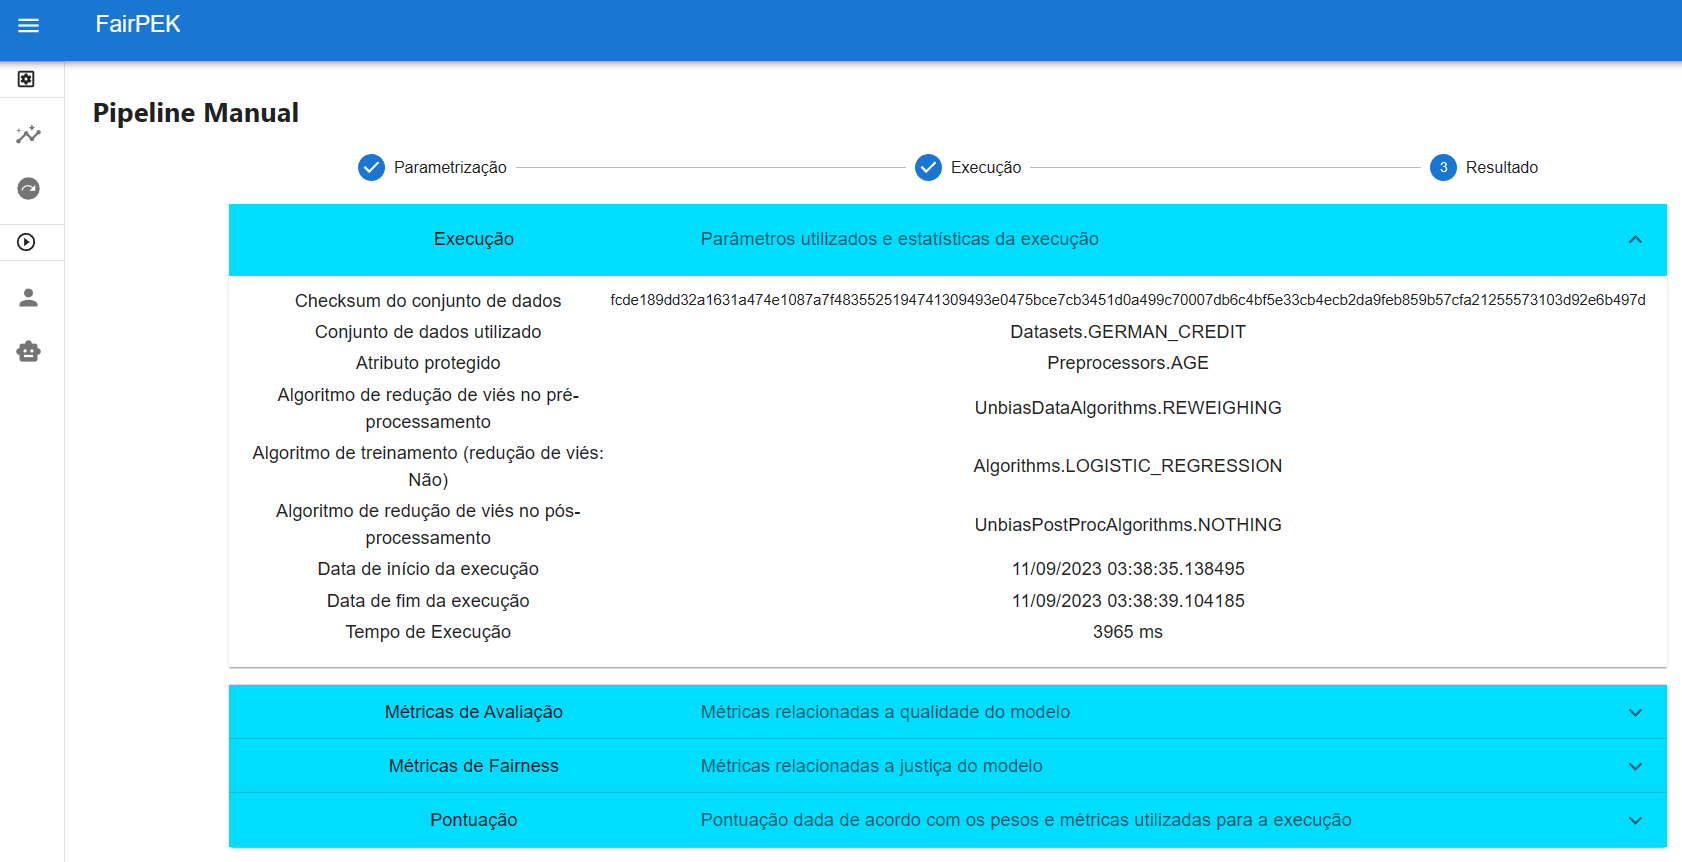
\includegraphics[scale=0.4]{images/front/Pipeline-Manual-Resultado-Parametros.png}}
    \subfigure[fig:pipelineManual2][Exibição das pontuações no resultado do workflow.]{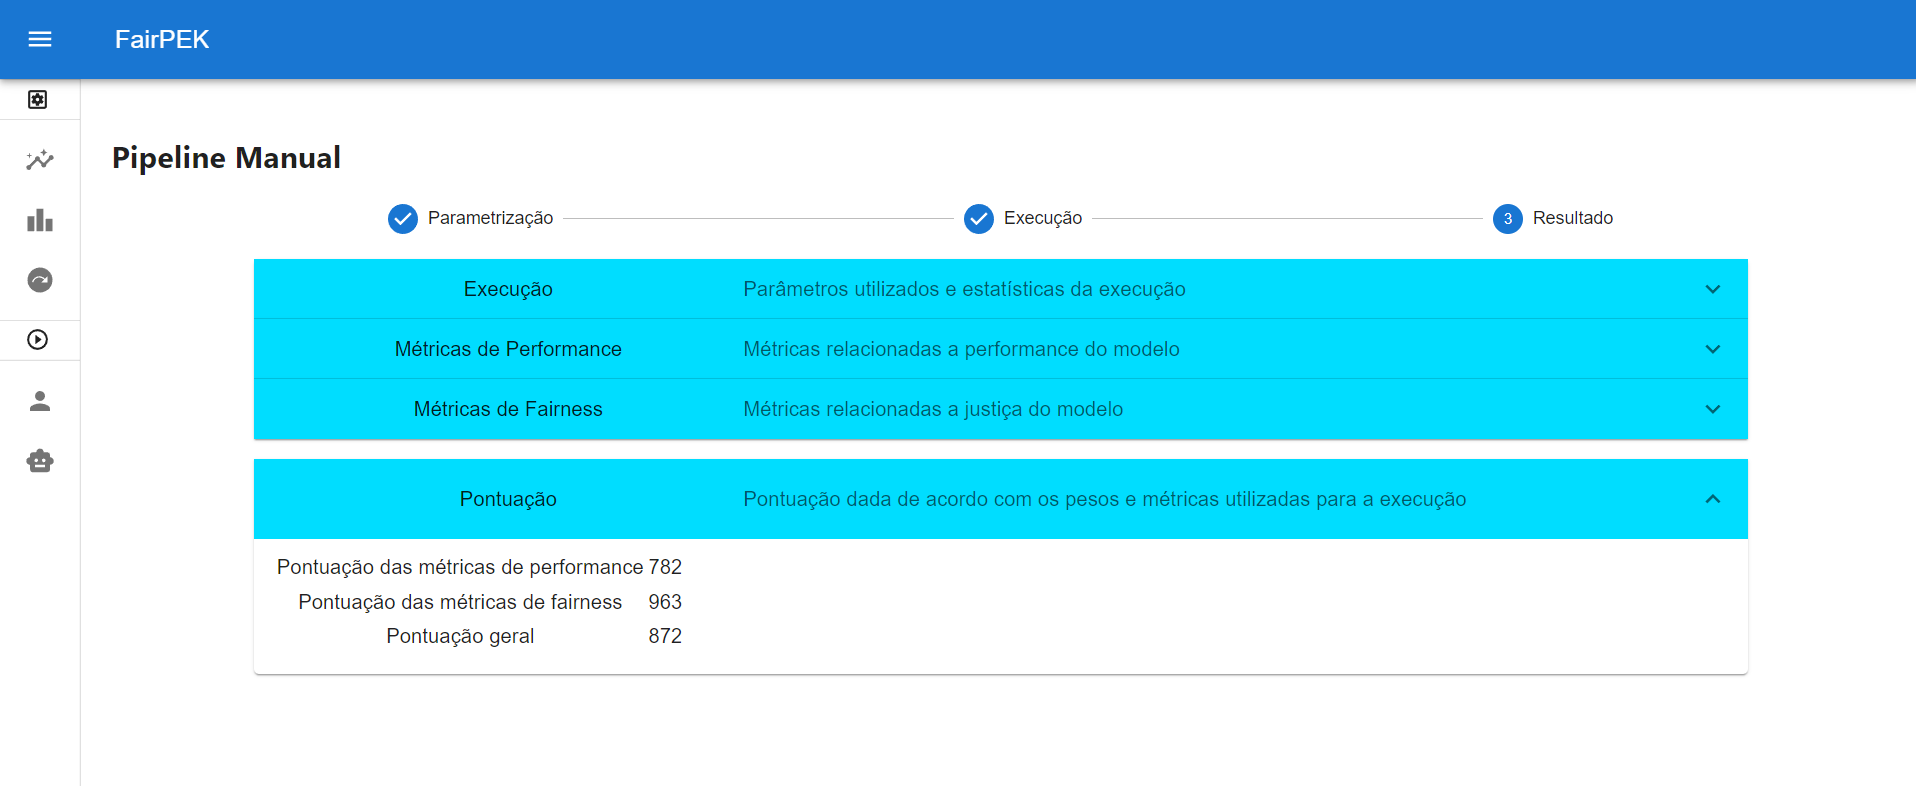
\includegraphics[scale=0.4]{images/front/Pipeline-Manual-Resultado-Pontuacao.png}}
    \caption{Informações do resultado do workflow.}
    \label{fig:pipelineManualInfo}
\end{figure}

\begin{figure}[H]
    \centering
    \subfigure[fig:pipelineManual1][Exibição das métricas de performance no resultado do workflow.]{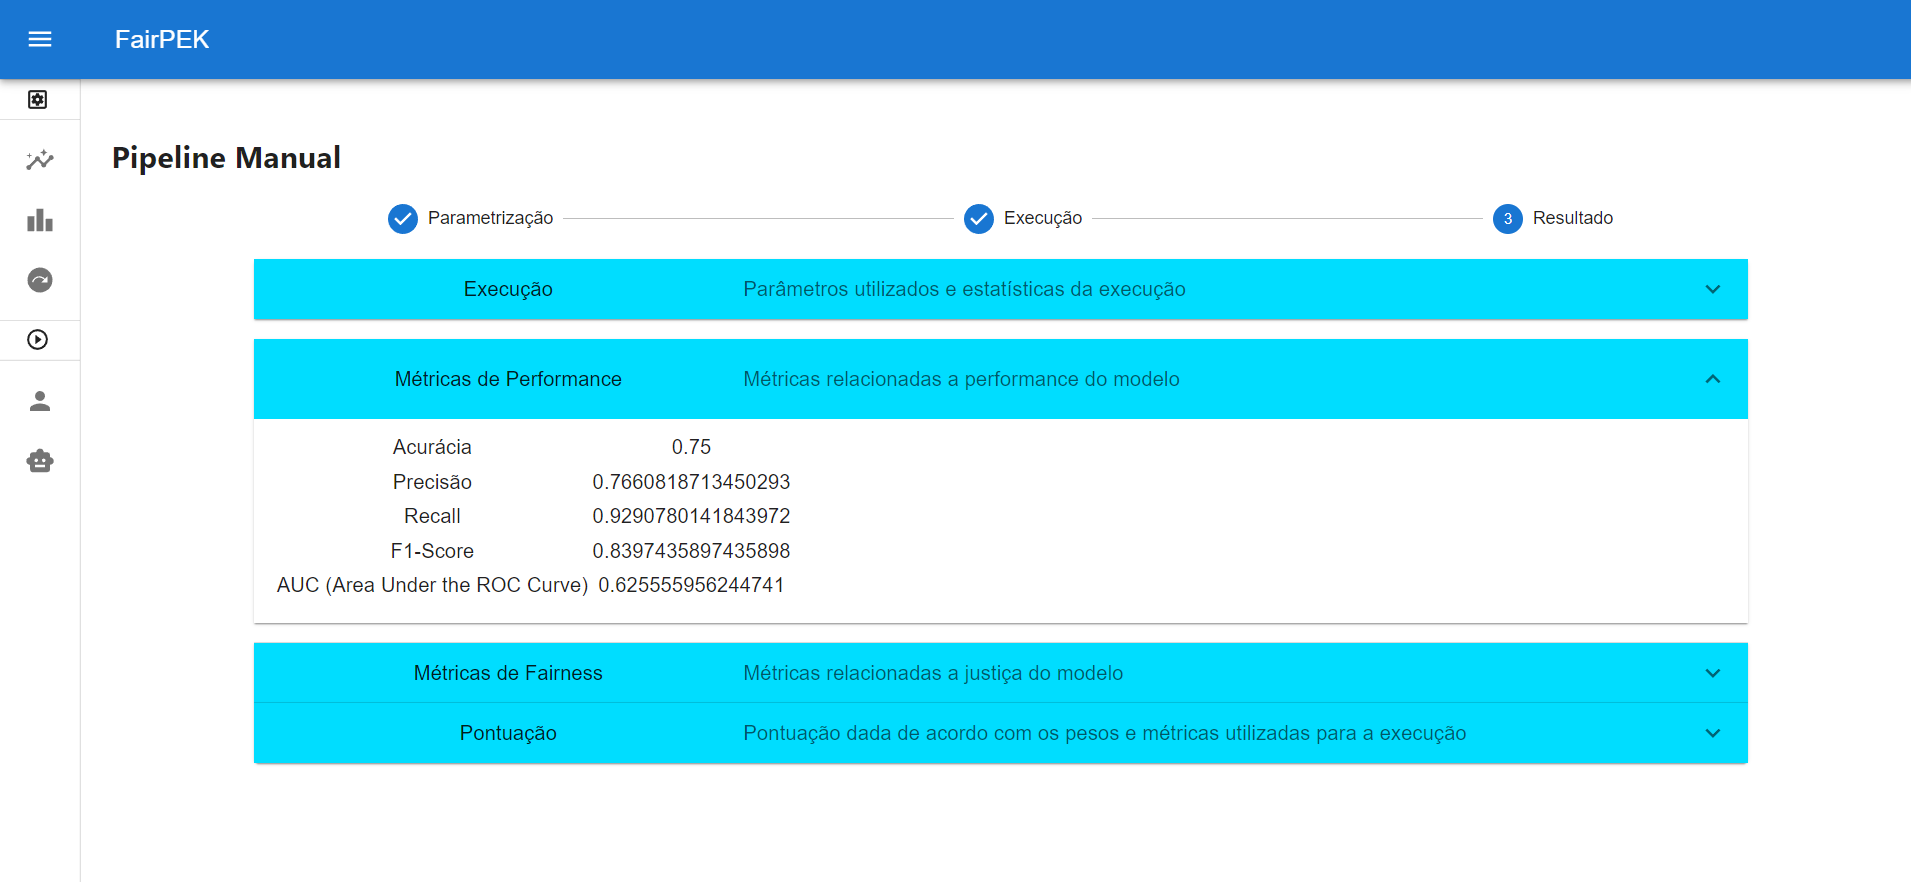
\includegraphics[scale=0.4]{images/front/Pipeline-Manual-Resultado-Metricas-Performance.png}}
    \subfigure[fig:pipelineManual2][Exibição das métricas de fairness no resultado do workflow.]{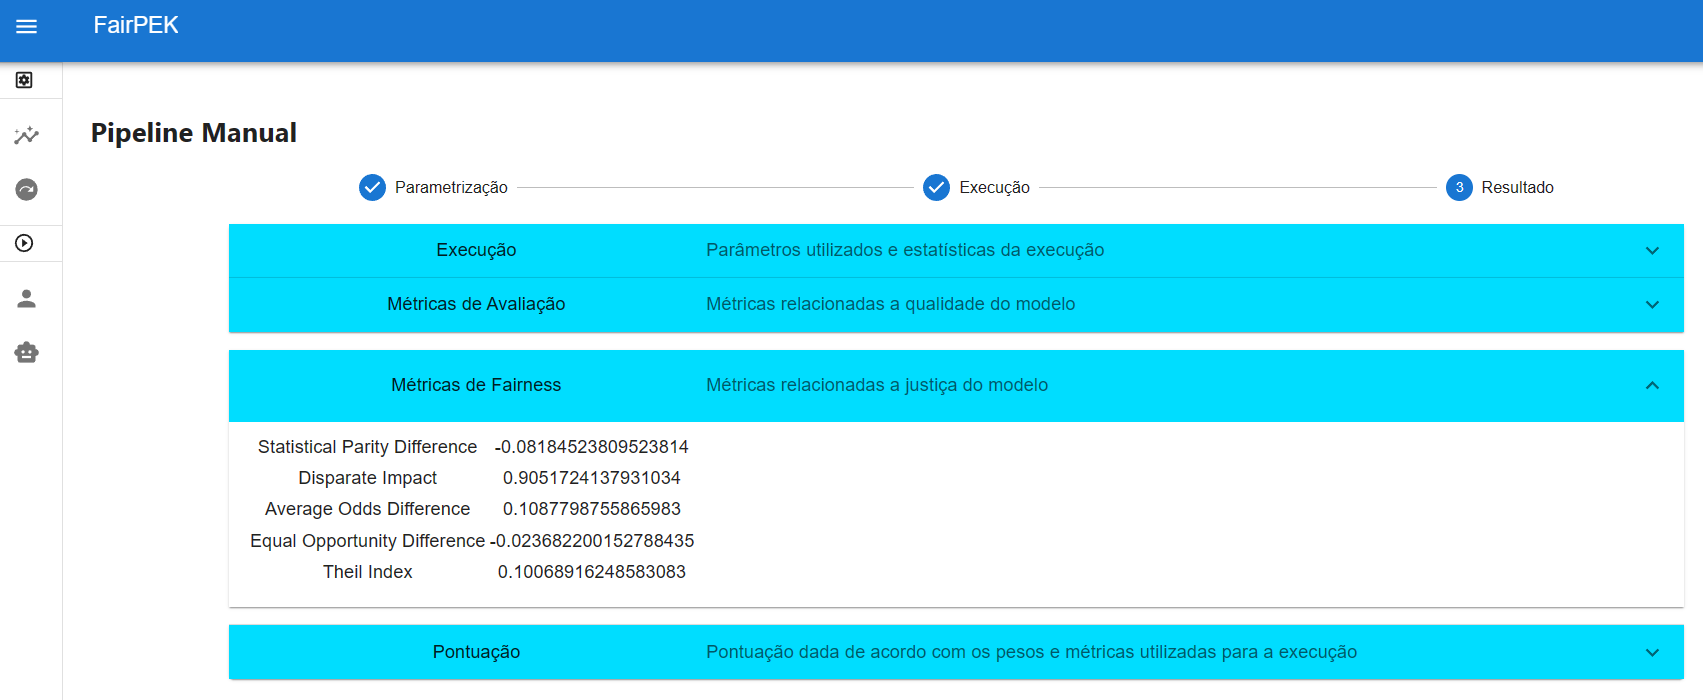
\includegraphics[scale=0.4]{images/front/Pipeline-Manual-Resultado-Metricas-Fairness.png}}
    \caption{Métricas do resultado do workflow.}
    \label{fig:pipelineManualMetricas}
\end{figure}

\subsubsection{Execução autônoma do Workflow}

Ao clicar a opção do menu "Pipeline Autônomo", é exibida a tela ilustrada na Figura \ref{fig:pipelineAutonomo}. Ela possui indicações de etapas divididas em Parametrização, Análise, Opções, Execução e Resultados e um campo para selecionar o conjunto de dados. Ao clicar no botão "Executar" localizado no canto superior direito, é feita uma requisição para escolher o melhor conjunto de parâmetros baseado em execuções anteriores, é exibida uma indicação de sucesso no canto inferior esquerdo e a indicação de etapa é atualizada para a etapa de análise.

\begin{figure}[H]
    \centering
    \subfigure[fig:pipelineAutonomo1][Opções para configurar o workflow de forma autônoma.]{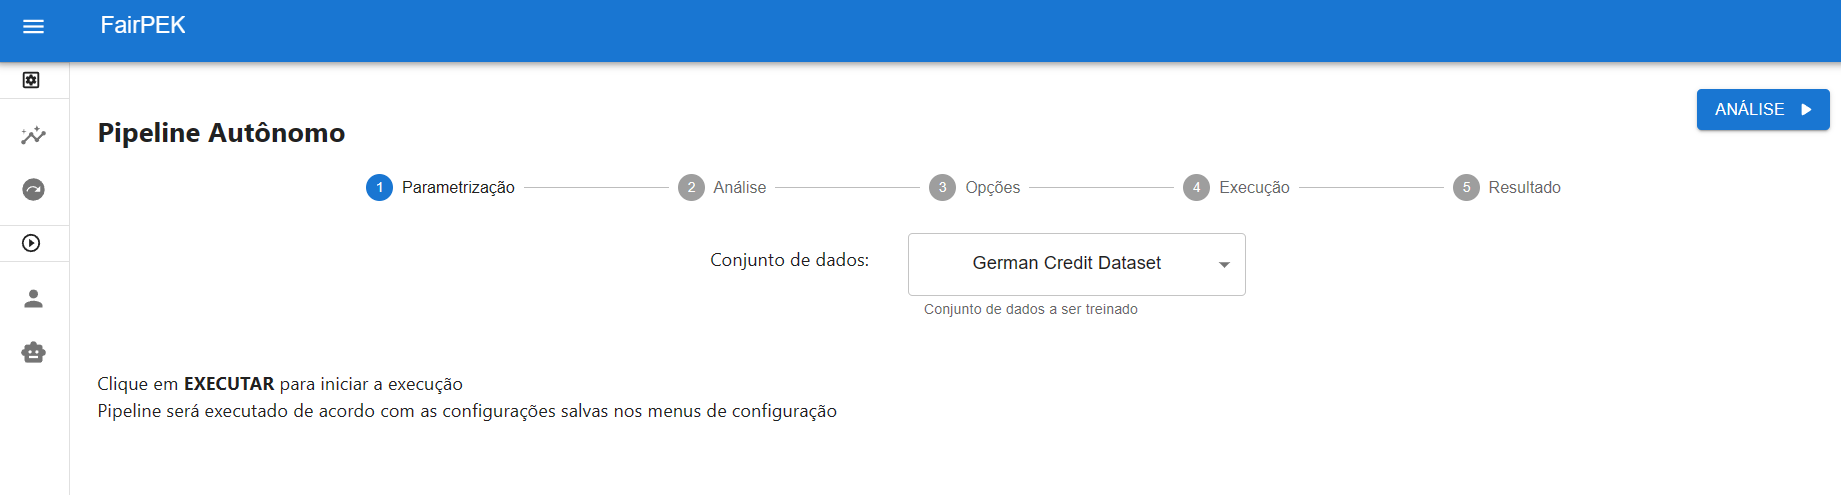
\includegraphics[scale=0.4]{images/front/Pipeline-Autonomo-Parametros.png}}
    \subfigure[fig:pipelineAutonomo2][Análise do Gerenciador Autonômico em execução.]{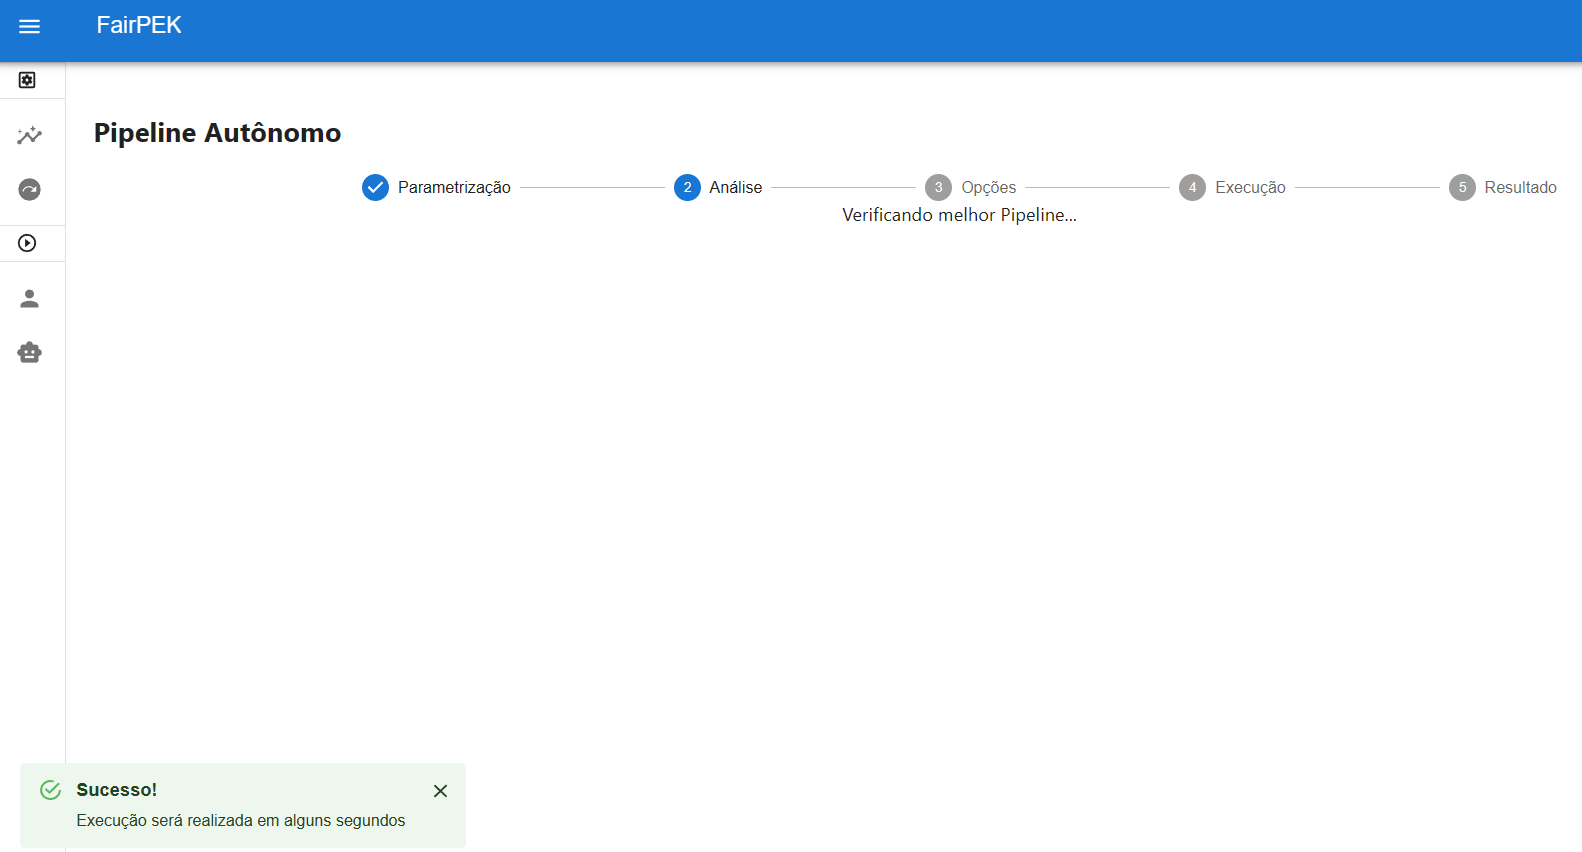
\includegraphics[scale=0.4]{images/front/Pipeline-Autonomo-Analise.png}}
    \caption{Execução autônoma do Workflow.}
    \label{fig:pipelineAutonomo}
\end{figure}

Após a etapa de análise ser concluída, a indicação de etapa é atualizada para a etapa de opções, conforme ilustração na Figura \ref{fig:pipelineAutonomoSelecao}. Nela, os parâmetros sugeridos são organizados nos mesmos grupos presentes nas Figuras \ref{fig:pipelineManualInfo} e \ref{fig:pipelineManualMetricas} e podem ser consultados para selecionar a melhor escolha possível das 5 melhores sugestões de acordo com a pontuação calculada, podendo contestar ou não a melhor escolha sugerida pelo Gerenciador Autonômico.

\begin{figure}[H]
    \centering
    \subfigure[fig:pipelineAutonomoSelecao1][Opções para seleção de workflow para execução.]{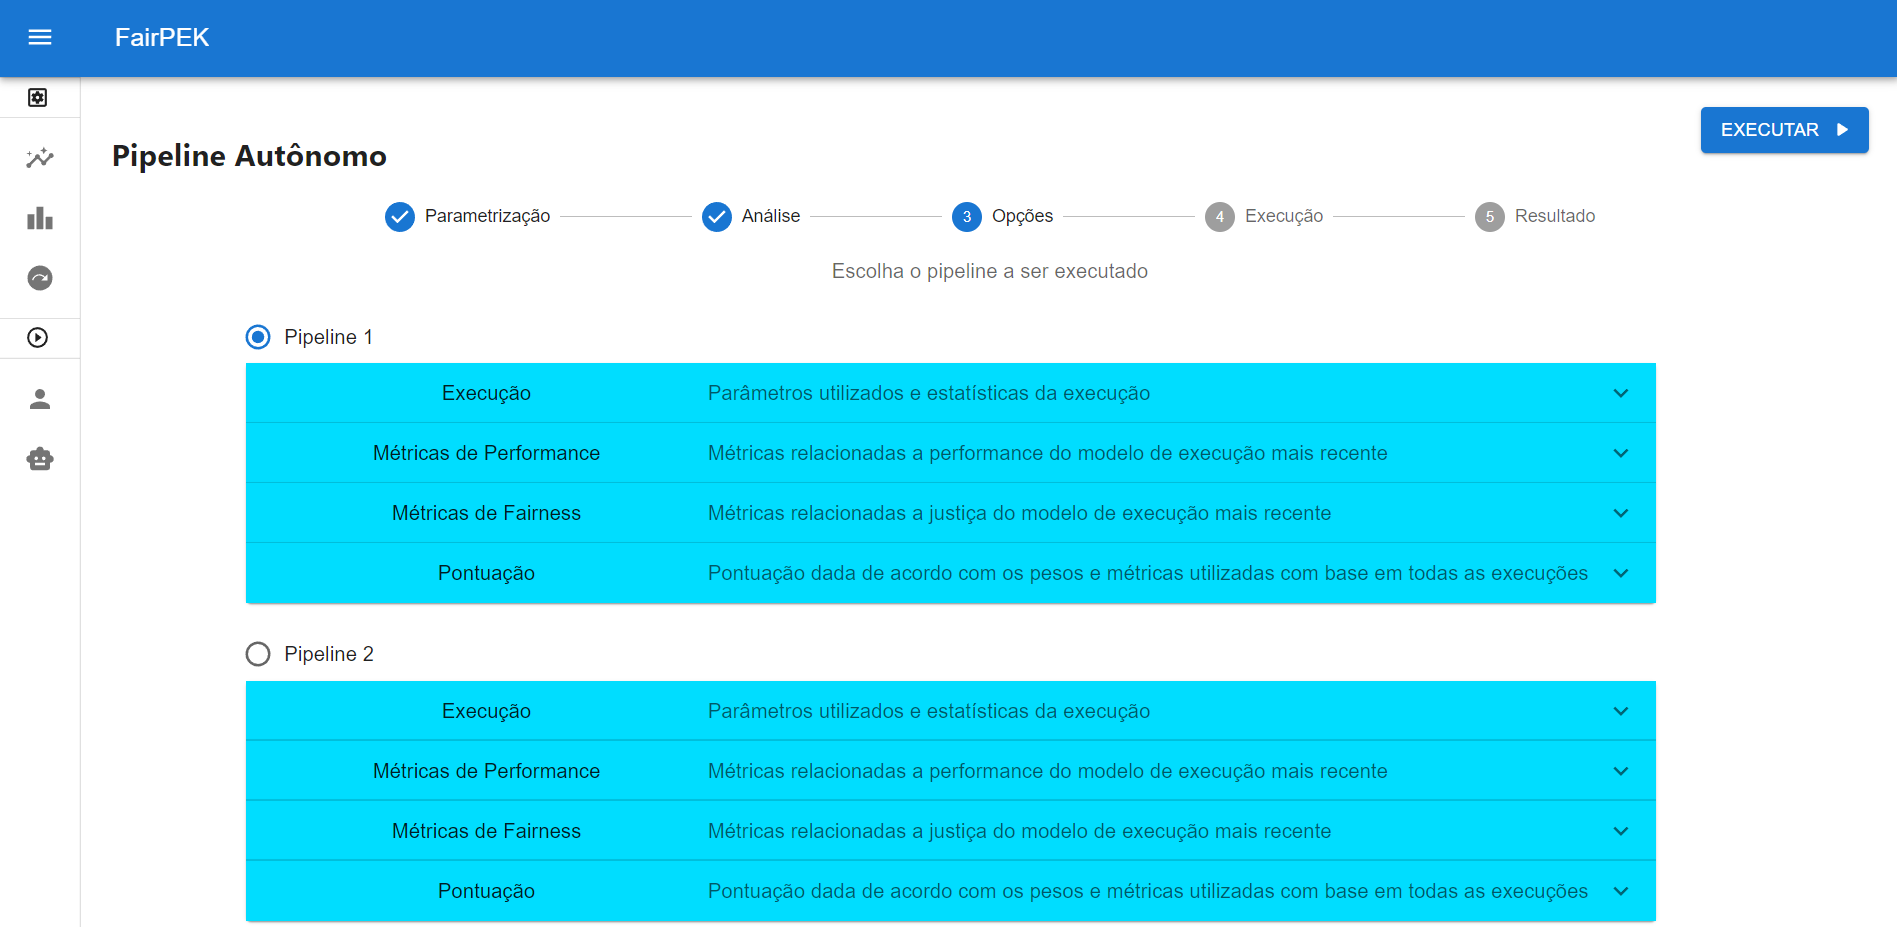
\includegraphics[scale=0.4]{images/front/Pipeline-Autonomo-Selecao.png}}
    \subfigure[fig:pipelineAutonomoSelecao2][Parâmetros a serem utilizados para execução.]{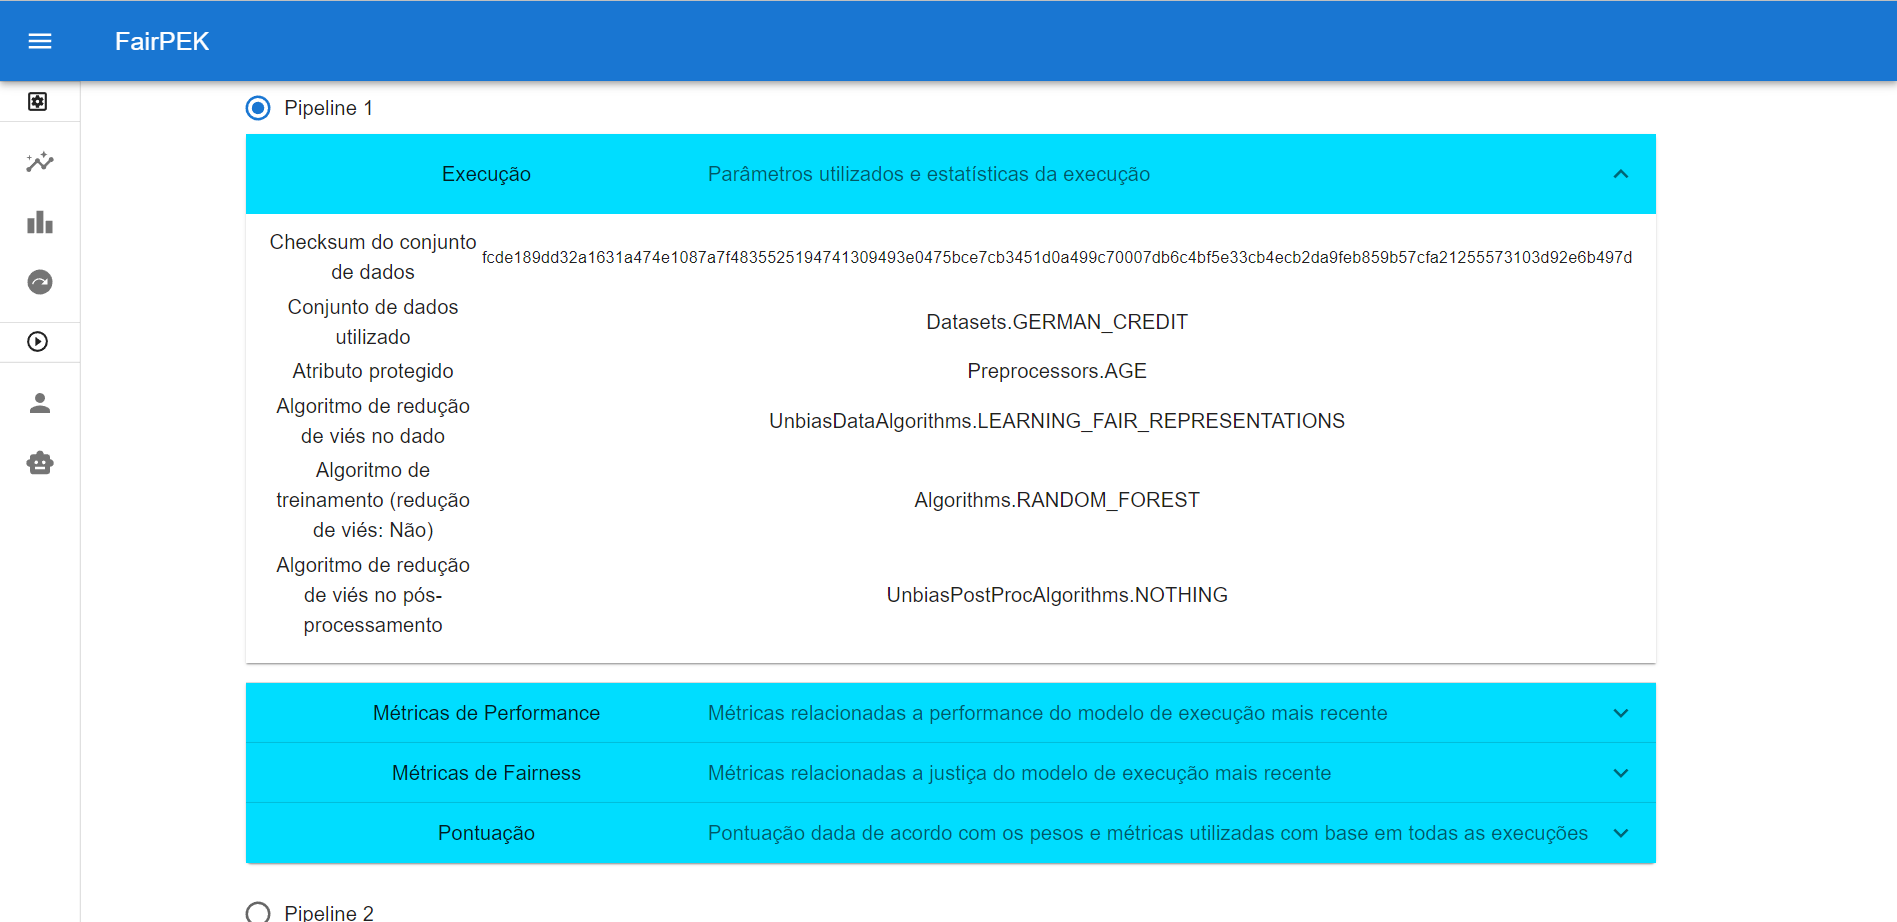
\includegraphics[scale=0.4]{images/front/Pipeline-Autonomo-Selecao-Parametros.png}}
    \caption{Seleção do workflow após análise.}
    \label{fig:pipelineAutonomoSelecao}
\end{figure}

Ao clicar novamente no botão "Executar" localizado no canto superior direito, é feita uma requisição para executar o \textit{Workflow} com a opção selecionada, e a indicação de etapa é atualizada para a etapa de execução. Após a execução ser concluída,  a indicação de etapa é atualizada para a etapa de resultados, conforme ilustração na Figura \ref{fig:pipelineAutonomoResultado}. Nela, os parâmetros sugeridos são organizados nos mesmos grupos presentes na Figura \ref{fig:pipelineAutonomoSelecao}, mas desta vez refletem as métricas e pontuação da execução realizada pelo \textit{Workflow}.

,
\begin{figure}[H]
    \centering
    \subfigure[fig:pipelineAutonomoResultado1][Workflow em execução.]{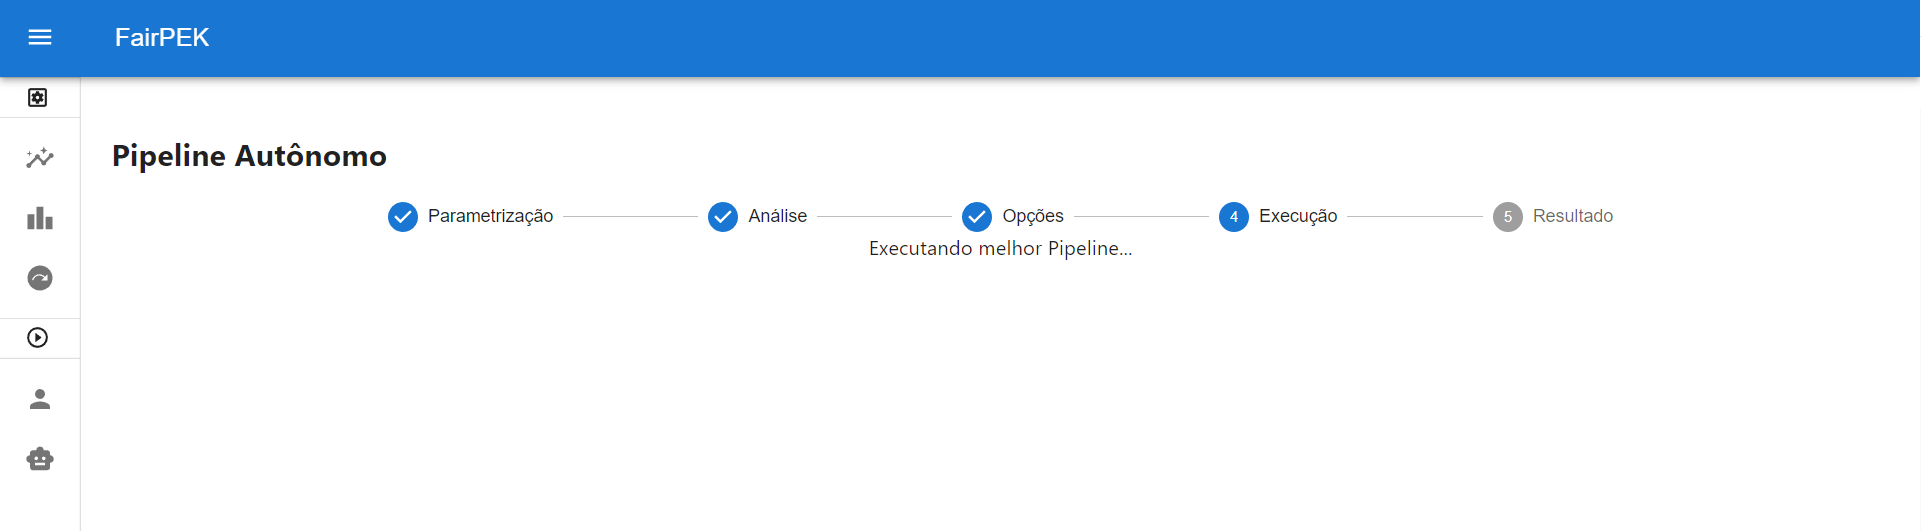
\includegraphics[scale=0.4]{images/front/Pipeline-Autonomo-Execucao.png}}
    \subfigure[fig:pipelineAutonomoResultado2][Resultados da execução realizada.]{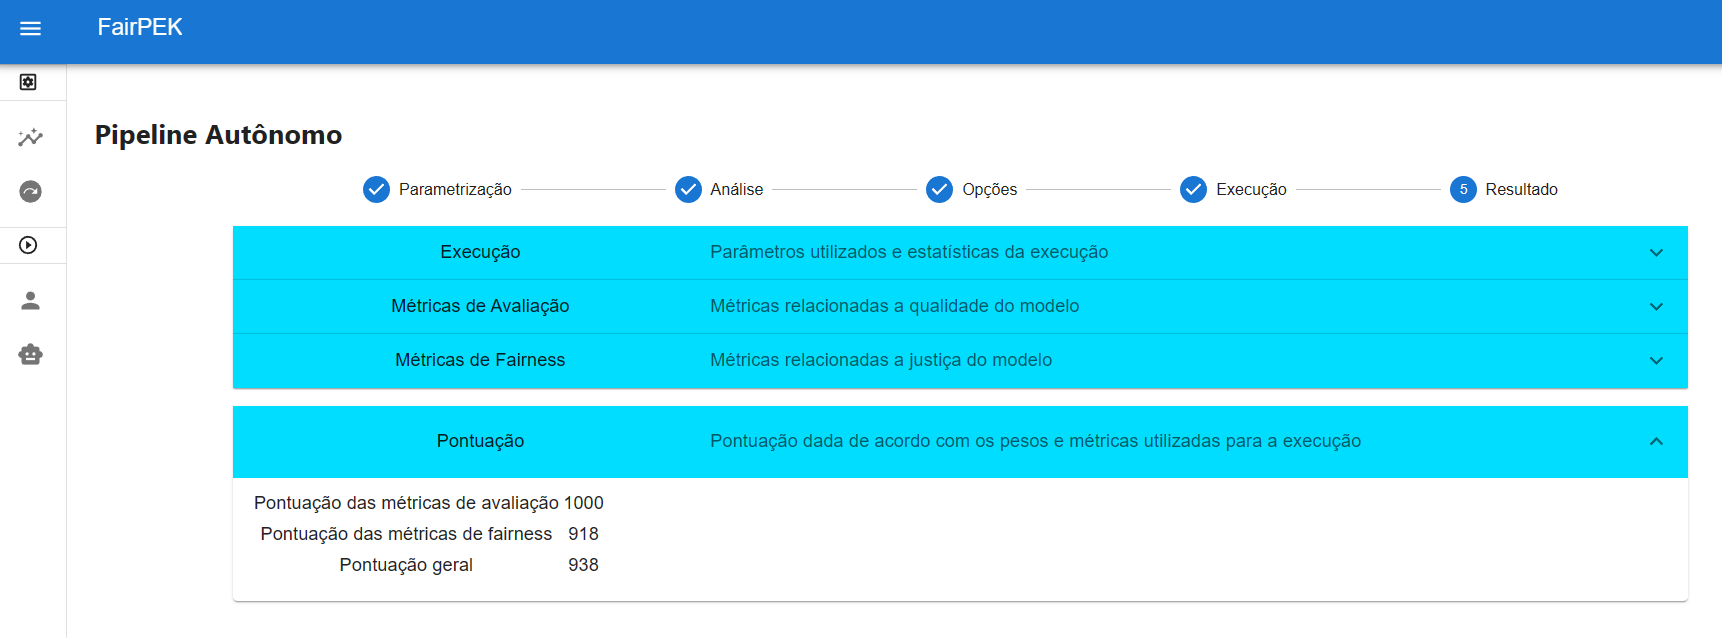
\includegraphics[scale=0.4]{images/front/Pipeline-Autonomo-Resultado.png}}
    \caption{Execução do workflow após seleção.}
    \label{fig:pipelineAutonomoResultado}
\end{figure}

\chapter{Estudo de Caso 1: Classificação de Crédito (German Credit Dataset)}

Neste Estudo de Caso, o maior foco foi colocado em testar e verificar como o \mbox{MAPE-K} se comporta em um cenário com diversas execuções prévias de \textit{Workflows}. Como as execuções geraram uma base de conhecimento, o Gerenciador Autonômico pode executar uma análise através destes dados e determinar um plano indicando a gama de algoritmos que utilizará para obter melhores resultados. Foram notados resultados em outras escolhas realizadas para a construção desta aplicação, mas que serão melhor discutidos nos estudos seguintes.

\section{Contexto e limitações}

O experimento foi realizado com o seguinte conjunto de dados e dado o seguinte contexto:

\begin{itemize}
\item \textbf{Contexto:} Obter classificação de crédito (boa ou ruim), através de uma série de \textit{features}

\item \textbf{Conjunto de dados:} German Credit Dataset, presente em \citep{ucigerman_2021}.

\item \textbf{Transformações realizadas no conjunto de dados:} Mudanças nos valores dos atributos para valores de interpretação mais simples, para que o Cientista de Dados possa categorizar o dado posteriormente e de forma mais fácil no \textit{Workflow}.

\item \textbf{Atributos protegidos:} Idade ou Nacionalidade

\item \textbf{Grupo privilegiado:} Idade maior ou igual a 25 anos; Nacionalidade Alemã

\item \textbf{Grupo não-privilegiado:} Idade menor que 25 anos; Nacionalidade diferente da Alemã (Estrangeiro)

\end{itemize}

Para realizar este experimento, foi considerado o seguinte objetivo e consideradas as seguintes limitações:

\begin{itemize}
\item \textbf{Experimento:} Execução de um \textit{workflow} de ML para obtenção de dados iniciais na base de conhecimento e discussão de um \textit{workflow} de ML utilizando MAPE-K como facilitador da escolha de modelo.

\item \textbf{Medição:} Serão medidas as pontuações de cada agrupamento de métricas (Performance e Fairness), e tais métricas também serão comparadas com o valor de cada uma para verificar seu impacto na pontuação.

\item \textbf{Obtenção dos dados:} A execução do \textit{Pipeline} utilizando o Gerenciador Autonômico foi realizada com 3 pesagens diferentes na pontuação geral:

\begin{itemize}
\item 50\% para métricas de Performance e 50\% para métricas de Fairness, para uma configuração equilibrada.
\item 75\% para métricas de Performance e 25\% para métricas de Fairness, para uma configuração que prioriza a performance em detrimento da justiça.
\item 25\% para métricas de Performance e 75\% para métricas de Fairness, para uma configuração que prioriza a justiça em detrimento da performance.
\end{itemize}

Em todas as execuções são utilizadas as métricas Acurácia, Precisão, \textit{Recall}, \textit{F1-Score} e AUC como métricas de Performance e as métricas \textit{Statistical Parity Difference}, \textit{Equal Opportunity Difference}, \textit{Average Odds Difference}, \textit{Disparate Impact} e \textit{Theil Index} como métricas de \textit{Fairness}, todas com pesagens iguais em seu respectivo agrupamento.

\item \textbf{Pré-condição 1:} Houveram \textit{workflows} que já foram pré-executados e já formaram uma base de conhecimento. Para o experimento, foi considerado ao menos 1 execução para cada combinação de conjunto de dados, atributo protegido e algoritmos utilizados.

\item \textbf{Pré-condição 2:} A base de conhecimento gerada para uso do MAPE-K terá atributos para verificar performance a imparcialidade/justiça de um modelo, mas não terá atributos para verificar a influência de cada \textit{feature} aplicada no modelo.

\item \textbf{Pré-condição 3:} Podem existir ruídos nos resultados finais devido ao German Credit Dataset ser uma base de dados com poucas amostras (apenas 1000), mas eles serão desconsiderados uma vez que o conjunto de dados ainda é considerado como \textit{benchmark} em alguns trabalhos acadêmicos \citep{Kamiran_2011}~\citep{Feldman_2015}~\citep{Celis_2019} e seus dados exemplificam muito bem uma situação real onde dados sensíveis podem ser utilizados e são possíveis de afetar a decisão de um modelo e, consequentemente, a situação de vida de uma pessoa.

\item \textbf{Restrição 1:} O algoritmo de retirada de viés é feito em apenas uma parte das etapas (Pré-processamento/Processamento/Pós-processamento). Isto foi decidido pois não foram verificadas referências onde a aplicação desses algortimos em duas ou em todas as três etapas impacta em melhora nas métricas de \textit{Fairness}.

\item \textbf{Restrição 2:} Por não conseguirem rodar com sucesso, foram retirados os \textit{Workflows} que rodaram os seguintes algoritmos: Pré-processamento Otimizado.

\item \textbf{Restrição 3:} \textit{Workflows} também foram retirados por apresentarem métricas com valores máximos, para evitar análises caso exista alguma falha não detectada na implementação. Como exemplo, os que possuíam Classificação baseada em Rejeição de Opções.

\item \textbf{Restrição 4:} Para evitar \textit{workflows} com conjuntos de algoritmos ruins e também pelo mesmo motivo da restrição anterior, o intervalo de pontuação para análise foi limitado de 500 a 950.
\end{itemize}

\section{Resultados e Discussões}

Os resultados baseados nas pré-condições e restrições já comentadas na seção anterior estão presentes abaixo nas Tabelas \ref{tbl:ScoreMAPEKGeral5050}, \ref{tbl:ScoreMAPEKGeral7525} e \ref{tbl:ScoreMAPEKGeral2575}:

\begin{table}[H]
\begin{center}
  \caption{Melhores opções escolhidas pelo modelo MAPE-K \\ Todos os métodos - 50\% Performance/50\% Fairness}
\label{tbl:ScoreMAPEKGeral5050}
  \resizebox{\linewidth}{!}{%
\begin{tabular}{c|c|c|c|c|c|c}
\multicolumn{4}{c|}{Workflow} & \multicolumn{3}{c}{Pontuação} \\
\hline
Atributo protegido & Pré-processamento & Treinamento & Pós-processamento & Performance & Fairness & \textbf{Geral} \\
\hline
Idade & Nenhum & Regressão Logística & Equalized Odds & 968 & 860 & \textbf{914} \\
Nacionalidade & Nenhum & Random Forest & Calibrated Equalized Odds & 902 & 922 & \textbf{912} \\
Nacionalidade & Nenhum & Gradient Boosting & Calibrated Equalized Odds & 870 & 925 & \textbf{898} \\
Idade & Nenhum & Gradient Boosting & Equalized Odds & 927 & 862 & \textbf{894} \\
Idade & Reweighing & Gradient Boosting & Nenhum & 804 & 931 & \textbf{868} \\
\end{tabular}}
\end{center}
\end{table}

\begin{table}[H]
\begin{center}
  \caption{Melhores opções escolhidas pelo modelo MAPE-K \\ Todos os métodos - 75\% Performance/25\% Fairness}
\label{tbl:ScoreMAPEKGeral7525}
  \resizebox{\linewidth}{!}{%
\begin{tabular}{c|c|c|c|c|c|c}
\multicolumn{4}{c|}{Workflow} & \multicolumn{3}{c}{Pontuação} \\
\hline
Atributo protegido & Pré-processamento & Treinamento & Pós-processamento & Performance & Fairness & \textbf{Geral} \\
\hline
Idade & Nenhum & Regressão Logística & Equalized Odds & 968 & 860 & \textbf{941} \\
Idade & Nenhum & Gradient Boosting & Equalized Odds & 927 & 862 & \textbf{910} \\
Nacionalidade & Nenhum & Random Forest & Calibrated Equalized Odds & 902 & 922 & \textbf{907} \\
Nacionalidade & Nenhum & Gradient Boosting & Calibrated Equalized Odds & 870 & 925 & \textbf{883} \\
Idade & Nenhum & Random Forest & Equalized Odds & 898 & 799 & \textbf{874} \\
\end{tabular}}
\end{center}
\end{table}

\begin{table}[H]
\begin{center}
  \caption{Melhores opções escolhidas pelo modelo MAPE-K \\ Todos os métodos - 25\% Performance/75\% Fairness}
\label{tbl:ScoreMAPEKGeral2575}
  \resizebox{\linewidth}{!}{%
\begin{tabular}{c|c|c|c|c|c|c}
\multicolumn{4}{c|}{Workflow} & \multicolumn{3}{c}{Pontuação} \\
\hline
Atributo protegido & Pré-processamento & Treinamento & Pós-processamento & Performance & Fairness & \textbf{Geral} \\
\hline
Idade & Disparate Impact Remover & Support Vector Machines & Nenhum & 747 & 989 & \textbf{928} \\
Nacionalidade & Disparate Impact Remover & Support Vector Machines & Nenhum & 747 & 989 & \textbf{928} \\
Idade & Nenhum & Adversarial Debiasing & Nenhum & 742 & 979 & \textbf{920} \\
Nacionalidade & Reweighing & Support Vector Machines & Nenhum & 755 & 972 & \textbf{918} \\
Nacionalidade & Learning Fair Representations & Support Vector Machines & Nenhum & 755 & 972 & \textbf{918} \\
\end{tabular}}
\end{center}
\end{table}

Nessas execuções, surpreende 2 observações. A primeira é o fato da predominância de algoritmos com redução de viés na etapa de pós-processamento especialmente em configurações que priorizavam performance, contrariando o esperado de que os algoritmos com redução de viés aumentavam justiça em detrimento da performance. A segunda é a predominância de algoritmos com redução de viés na etapa de pré-processamento em configurações que priorizavam justiça, principalmente pois todos as execuções usavam \textit{Support Vector Machines} como algoritmo de treinamento.

Diante destas 2 predominâncias envolvendo todos os \textit{workflows} executados, novos experimentos com restrições adicionais foram realizados para obter observações mais detalhadas a respeito dos resultados:

\begin{itemize}
\item Uso apenas de \textit{workflows} com o uso de algoritmos com redução de viés na etapa de \mbox{pré-processamento} (manipulação de dados).
\item Uso apenas de \textit{workflows} com o uso de algoritmos com redução de viés no \mbox{processamento} (treinamento).
\item Uso apenas de \textit{workflows} com o uso de algoritmos com redução de viés no \mbox{pós-processamento} (manipulação do resultado final).
\item Uso apenas de \textit{workflows} sem o uso de algoritmos com redução de viés.
\end{itemize}

As pré-condições, restrições e pesagens nas pontuações usadas anteriormente foram mantidas e seus resultados estão presentes abaixo nas Tabelas \ref{tbl:ScoreMAPEKPreproc5050}, \ref{tbl:ScoreMAPEKPreproc7525}, \ref{tbl:ScoreMAPEKPreproc2575}, \ref{tbl:ScoreMAPEKInproc5050}, \ref{tbl:ScoreMAPEKInproc7525}, \ref{tbl:ScoreMAPEKInproc2575}, \ref{tbl:ScoreMAPEKPostproc5050}, \ref{tbl:ScoreMAPEKPostproc7525}, \ref{tbl:ScoreMAPEKPostproc2575}, \ref{tbl:ScoreMAPEKNoproc5050}, \ref{tbl:ScoreMAPEKNoproc7525} e \ref{tbl:ScoreMAPEKNoproc2575}:

\begin{table}[H]
\begin{center}
  \caption{Melhores opções escolhidas pelo modelo MAPE-K \\ Apenas com redução de viés no dado - 50\% Performance/50\% Fairness}
\label{tbl:ScoreMAPEKPreproc5050}
  \resizebox{\linewidth}{!}{%
\begin{tabular}{c|c|c|c|c|c|c}
\multicolumn{4}{c|}{Workflow} & \multicolumn{3}{c}{Pontuação} \\
\hline
Atributo protegido & Pré-processamento & Treinamento & Pós-processamento & Performance & Fairness & \textbf{Geral} \\
\hline
Idade & Reweighing & Gradient Boosting & Nenhum & 804 & 931 & \textbf{868} \\
Idade & Learning Fair Representations & Gradient Boosting & Nenhum & 804 & 931 & \textbf{868} \\
Idade & Disparate Impact Remover & Support Vector Machines & Nenhum & 747 & 989 & \textbf{868} \\
Nacionalidade & Disparate Impact Remover & Support Vector Machines & Nenhum & 747 & 989 & \textbf{868} \\
Nacionalidade & Learning Fair Representations & Support Vector Machines & Nenhum & 755 & 972 & \textbf{864} \\
\end{tabular}}
\end{center}
\end{table}

\begin{table}[H]
\begin{center}
  \caption{Melhores opções escolhidas pelo modelo MAPE-K \\ Apenas com redução de viés no dado - 75\% Performance/25\% Fairness}
\label{tbl:ScoreMAPEKPreproc7525}
  \resizebox{\linewidth}{!}{%
\begin{tabular}{c|c|c|c|c|c|c}
\multicolumn{4}{c|}{Workflow} & \multicolumn{3}{c}{Pontuação} \\
\hline
Atributo protegido & Pré-processamento & Treinamento & Pós-processamento & Performance & Fairness & \textbf{Geral} \\
\hline
Idade & Reweighing & Gradient Boosting & Nenhum & 804 & 931 & \textbf{836} \\
Idade & Learning Fair Representations & Gradient Boosting & Nenhum & 804 & 931 & \textbf{836} \\
Nacionalidade & Learning Fair Representations & Gradient Boosting & Nenhum & 811 & 878 & \textbf{828} \\
Nacionalidade & Reweighing & Gradient Boosting & Nenhum & 811 & 878 & \textbf{828} \\
Nacionalidade & Learning Fair Representations & Random Forest & Nenhum & 801 & 883 & \textbf{821} \\
\end{tabular}}
\end{center}
\end{table}

\begin{table}[H]
\begin{center}
  \caption{Melhores opções escolhidas pelo modelo MAPE-K \\ Apenas com redução de viés no dado - 25\% Performance/75\% Fairness}
\label{tbl:ScoreMAPEKPreproc2575}
  \resizebox{\linewidth}{!}{%
\begin{tabular}{c|c|c|c|c|c|c}
\multicolumn{4}{c|}{Workflow} & \multicolumn{3}{c}{Pontuação} \\
\hline
Atributo protegido & Pré-processamento & Treinamento & Pós-processamento & Performance & Fairness & \textbf{Geral} \\
\hline
Idade & Disparate Impact Remover & Support Vector Machines & Nenhum & 747 & 989 & \textbf{928} \\
Nacionalidade & Disparate Impact Remover & Support Vector Machines & Nenhum & 747 & 989 & \textbf{928} \\
Nacionalidade & Learning Fair Representations & Support Vector Machines & Nenhum & 755 & 972 & \textbf{918} \\
Nacionalidade & Reweighing & Support Vector Machines & Nenhum & 755 & 972 & \textbf{918} \\
Idade & Learning Fair Representations & Support Vector Machines & Nenhum & 755 & 969 & \textbf{916} \\
\end{tabular}}
\end{center}
\end{table}

Nos \textit{workflows} utilizando apenas algoritmos com redução de viés no dado, percebe-se a predominância dos algoritmos de treinamento \textit{Gradient Boosting} e \textit{Support Vector Machines}, sendo o \textit{Gradient Boosting} predominante em configurações priorizando performance e o \textit{Support Vector Machines} predominante em configurações priorizando justiça, o que começa a explicar a sua predominância também presente no resultado geral. Também é possível perceber mais 2 observações: A primeira observação é que a análise de apenas uma categoria de algoritmos dá mais clareza em ver como o cálculo utilizado nas 3 configurações faz com que o equilíbrio de ambas as métricas se torna mais importante do que a prioridade apenas em performance ou apenas em justiça, uma vez que há exemplos de conjuntos de algoritmos com pontuações ligeiramente maiores em performance que acabaram sendo pior avaliados pois a pontuação em \textit{Fairness} está bem menor, e vice-versa. A segunda observação é que o uso de um atributo protegido diferente (e, por consequência, com tratamento de dados diferente) e de um algoritmo de treinamento parecem impactar tanto quanto ou até mais que o próprio algoritmo com redução de viés no dado.

\begin{table}[H]
\begin{center}
  \caption{Melhores opções escolhidas pelo modelo MAPE-K \\ Apenas com redução de viés no treinamento - 50\% Performance/50\% Fairness}
\label{tbl:ScoreMAPEKInproc5050}
  \resizebox{\linewidth}{!}{%
\begin{tabular}{c|c|c|c|c|c|c}
\multicolumn{4}{c|}{Workflow} & \multicolumn{3}{c}{Pontuação} \\
\hline
Atributo protegido & Pré-processamento & Treinamento & Pós-processamento & Performance & Fairness & \textbf{Geral} \\
\hline
Idade & Nenhum & Adversarial Debiasing & Nenhum & 742 & 979 & \textbf{860} \\
Nacionalidade & Nenhum & Grid Search Reduction & Nenhum & 789 & 895 & \textbf{845} \\
Idade & Nenhum & Meta Fair Classifier & Nenhum & 776 & 910 & \textbf{843} \\
Idade & Nenhum & Exponentiated Gradient Reduction & Nenhum & 811 & 869 & \textbf{840} \\
Nacionalidade & Nenhum & Rich Subgroup Fairness & Nenhum & 791 & 856 & \textbf{824} \\
\end{tabular}}
\end{center}
\end{table}

\begin{table}[H]
\begin{center}
  \caption{Melhores opções escolhidas pelo modelo MAPE-K \\ Apenas com redução de viés no treinamento - 75\% Performance/25\% Fairness}
\label{tbl:ScoreMAPEKInproc7525}
  \resizebox{\linewidth}{!}{%
\begin{tabular}{c|c|c|c|c|c|c}
\multicolumn{4}{c|}{Workflow} & \multicolumn{3}{c}{Pontuação} \\
\hline
Atributo protegido & Pré-processamento & Treinamento & Pós-processamento & Performance & Fairness & \textbf{Geral} \\
\hline
Idade & Nenhum & Exponentiated Gradient Reduction & Nenhum & 811 & 869 & \textbf{826} \\
Nacionalidade & Nenhum & Grid Search Reduction & Nenhum & 789 & 895 & \textbf{820} \\
Idade & Nenhum & Meta Fair Classifier & Nenhum & 776 & 910 & \textbf{809} \\
Nacionalidade & Nenhum & Exponentiated Gradient Reduction & Nenhum & 807 & 810 & \textbf{808} \\
Nacionalidade & Nenhum & Rich Subgroup Fairness & Nenhum & 791 & 856 & \textbf{807} \\
\end{tabular}}
\end{center}
\end{table}

\begin{table}[H]
\begin{center}
  \caption{Melhores opções escolhidas pelo modelo MAPE-K \\ Apenas com redução de viés no treinamento - 25\% Performance/75\% Fairness}
\label{tbl:ScoreMAPEKInproc2575}
  \resizebox{\linewidth}{!}{%
\begin{tabular}{c|c|c|c|c|c|c}
\multicolumn{4}{c|}{Workflow} & \multicolumn{3}{c}{Pontuação} \\
\hline
Atributo protegido & Pré-processamento & Treinamento & Pós-processamento & Performance & Fairness & \textbf{Geral} \\
\hline
Idade & Nenhum & Adversarial Debiasing & Nenhum & 742 & 979 & \textbf{920} \\
Idade & Nenhum & Meta Fair Classifier & Nenhum & 776 & 910 & \textbf{876} \\
Nacionalidade & Nenhum & Grid Search Reduction & Nenhum & 795 & 895 & \textbf{870} \\
Idade & Nenhum & Exponentiated Gradient Reduction & Nenhum & 811 & 869 & \textbf{854} \\
Nacionalidade & Nenhum & Prejudice Remover & Nenhum & 770 & 874 & \textbf{848} \\
\end{tabular}}
\end{center}
\end{table}

Nos \textit{workflows} utilizando apenas algoritmos com redução de viés no treinamento, percebe-se uma variedade maior nos algoritmos, até porque não há usos de redução de viés em um pré ou um pós-processamento, com destaque para o \textit{Adversarial Debiasing} que foi bem avaliado pela pontuação alta em \textit{Fairness}. Nestes \textit{workflows}, as 2 observações percebidas nos \textit{workflows} utilizando apenas algoritmos com redução de viés no dado são reforçadas por uma maior variedade de pontuações e pelo algoritmo \textit{Exponentiated Gradient Reduction} com 2 exemplos diferentes na Tabela \ref{tbl:ScoreMAPEKInproc7525}, onde o uso da Nacionalidade como atributo protegido possui pontuações de performance e \textit{Fairness} piores que a Idade e conclundo que o processamento utilizado no atributo protegido pode afetar todas as métricas.

\begin{table}[H]
\begin{center}
  \caption{Melhores opções escolhidas pelo modelo MAPE-K \\ Apenas com redução de viés no resultado - 50\% Performance/50\% Fairness}
\label{tbl:ScoreMAPEKPostproc5050}
  \resizebox{\linewidth}{!}{%
\begin{tabular}{c|c|c|c|c|c|c}
\multicolumn{4}{c|}{Workflow} & \multicolumn{3}{c}{Pontuação} \\
\hline
Atributo protegido & Pré-processamento & Treinamento & Pós-processamento & Performance & Fairness & \textbf{Geral} \\
\hline
Idade & Nenhum & Regressão Logística & Equalized Odds & 968 & 860 & \textbf{914} \\
Nacionalidade & Nenhum & Random Forest & Calibrated Equalized Odds & 902 & 922 & \textbf{912} \\
Nacionalidade & Nenhum & Gradient Boosting & Calibrated Equalized Odds & 870 & 925 & \textbf{898} \\
Idade & Nenhum & Gradient Boosting & Equalized Odds & 927 & 862 & \textbf{894} \\
Idade & Nenhum & Random Forest & Equalized Odds & 898 & 799 & \textbf{849} \\
\end{tabular}}
\end{center}
\end{table}

\begin{table}[H]
\begin{center}
  \caption{Melhores opções escolhidas pelo modelo MAPE-K \\ Apenas com redução de viés no resultado - 75\% Performance/25\% Fairness}
\label{tbl:ScoreMAPEKPostproc7525}
  \resizebox{\linewidth}{!}{%
\begin{tabular}{c|c|c|c|c|c|c}
\multicolumn{4}{c|}{Workflow} & \multicolumn{3}{c}{Pontuação} \\
\hline
Atributo protegido & Pré-processamento & Treinamento & Pós-processamento & Performance & Fairness & \textbf{Geral} \\
\hline
Idade & Nenhum & Regressão Logística & Equalized Odds & 968 & 860 & \textbf{941} \\
Idade & Nenhum & Gradient Boosting & Equalized Odds & 927 & 862 & \textbf{910} \\
Nacionalidade & Nenhum & Random Forest & Calibrated Equalized Odds & 902 & 922 & \textbf{907} \\
Nacionalidade & Nenhum & Gradient Boosting & Calibrated Equalized Odds & 870 & 925 & \textbf{883} \\
Idade & Nenhum & Random Forest & Equalized Odds & 898 & 799 & \textbf{874} \\
\end{tabular}}
\end{center}
\end{table}

\begin{table}[H]
\begin{center}
  \caption{Melhores opções escolhidas pelo modelo MAPE-K \\ Apenas com redução de viés no resultado - 25\% Performance/75\% Fairness}
\label{tbl:ScoreMAPEKPostproc2575}
  \resizebox{\linewidth}{!}{%
\begin{tabular}{c|c|c|c|c|c|c}
\multicolumn{4}{c|}{Workflow} & \multicolumn{3}{c}{Pontuação} \\
\hline
Atributo protegido & Pré-processamento & Treinamento & Pós-processamento & Performance & Fairness & \textbf{Geral} \\
\hline
Nacionalidade & Nenhum & Random Forest & Calibrated Equalized Odds & 902 & 922 & \textbf{917} \\
Nacionalidade & Nenhum & Gradient Boosting & Calibrated Equalized Odds & 870 & 925 & \textbf{911} \\
Idade & Nenhum & Regressão Logística & Equalized Odds & 968 & 860 & \textbf{887} \\
Idade & Nenhum & Gradient Boosting & Equalized Odds & 927 & 862 & \textbf{878} \\
Idade & Nenhum & Random Forest & Equalized Odds & 898 & 799 & \textbf{824} \\
\end{tabular}}
\end{center}
\end{table}

Nos \textit{workflows} utilizando apenas algoritmos com redução de viés no resultado, surpreende o fato de que os \textit{workflows} obtiveram as melhores pontuações em Performance e as piores pontuações em \textit{Fairness}, podendo indicar uma característica dos algoritmos \textit{Equalized Odds} e \textit{Calibrated Equalized Odds}. Entretanto, por conta da grande melhora por parte das métricas de performance, estes \textit{workflows} possuem um maior equilíbrio entre Performance e \textit{Fairness} e acabam garantindo maiores pontuações na média, justificando as melhores pontuações nas primeiras execuções onde foram considerados todos os métodos. Fora isto, as demais observações anteriores também se aplicam nestas execuções.

\begin{table}[H]
\begin{center}
  \caption{Melhores opções escolhidas pelo modelo MAPE-K \\ Apenas sem redução de viés - 50\% Performance/50\% Fairness}
\label{tbl:ScoreMAPEKNoproc5050}
  \resizebox{\linewidth}{!}{%
\begin{tabular}{c|c|c|c|c|c|c}
\multicolumn{4}{c|}{Workflow} & \multicolumn{3}{c}{Pontuação} \\
\hline
Atributo protegido & Pré-processamento & Treinamento & Pós-processamento & Performance & Fairness & \textbf{Geral} \\
\hline
Nacionalidade & Nenhum & Support Vector Machines & Nenhum & 755 & 972 & \textbf{864} \\
Idade & Nenhum & Support Vector Machines & Nenhum & 755 & 969 & \textbf{862} \\
Nacionalidade & Nenhum & Random Forest & Nenhum & 802 & 885 & \textbf{844} \\
Nacionalidade & Nenhum & Regressão Logística & Nenhum & 782 & 865 & \textbf{824} \\
Nacionalidade & Nenhum & Gradient Boosting & Nenhum & 817 & 784 & \textbf{800} \\
\end{tabular}}
\end{center}
\end{table}

\begin{table}[H]
\begin{center}
  \caption{Melhores opções escolhidas pelo modelo MAPE-K \\ Apenas sem redução de viés - 75\% Performance/25\% Fairness}
\label{tbl:ScoreMAPEKNoproc7525}
  \resizebox{\linewidth}{!}{%
\begin{tabular}{c|c|c|c|c|c|c}
\multicolumn{4}{c|}{Workflow} & \multicolumn{3}{c}{Pontuação} \\
\hline
Atributo protegido & Pré-processamento & Treinamento & Pós-processamento & Performance & Fairness & \textbf{Geral} \\
\hline
Nacionalidade & Nenhum & Random Forest & Nenhum & 802 & 885 & \textbf{823} \\
Nacionalidade & Nenhum & Gradient Boosting & Nenhum & 817 & 784 & \textbf{809} \\
Nacionalidade & Nenhum & Support Vector Machines & Nenhum & 755 & 972 & \textbf{809} \\
Idade & Nenhum & Support Vector Machines & Nenhum & 755 & 969 & \textbf{808} \\
Idade & Nenhum & Gradient Boosting & Nenhum & 817 & 778 & \textbf{807} \\
\end{tabular}}
\end{center}
\end{table}

\begin{table}[H]
\begin{center}
  \caption{Melhores opções escolhidas pelo modelo MAPE-K \\ Apenas sem redução de viés - 25\% Performance/75\% Fairness}
\label{tbl:ScoreMAPEKNoproc2575}
  \resizebox{\linewidth}{!}{%
\begin{tabular}{c|c|c|c|c|c|c}
\multicolumn{4}{c|}{Workflow} & \multicolumn{3}{c}{Pontuação} \\
\hline
Atributo protegido & Pré-processamento & Treinamento & Pós-processamento & Performance & Fairness & \textbf{Geral} \\
\hline
Nacionalidade & Nenhum & Support Vector Machines & Nenhum & 755 & 972 & \textbf{918} \\
Idade & Nenhum & Support Vector Machines & Nenhum & 755 & 969 & \textbf{916} \\
Nacionalidade & Nenhum & Random Forest & Nenhum & 802 & 885 & \textbf{864} \\
Nacionalidade & Nenhum & Regressão Logística & Nenhum & 782 & 865 & \textbf{844} \\
Idade & Nenhum & Regressão Logística & Nenhum & 782 & 802 & \textbf{797} \\
\end{tabular}}
\end{center}
\end{table}

Olhando os \textit{workflows} sem algoritmos com redução de viés, é curioso notar que, ao comparar com \textit{workflows} equivalentes mas com algoritmos usando redução de viés no dado, é possível notar que a hipótese principal se confirma em sua grande maioria: As pontuações em Performance são ligeiramente maiores e as pontuações em \textit{Fairness} são ligeiramente menores. É possível notar uma exceção no \textit{workflow} envolvendo o algoritmo \textit{Random Forest}, mas nos outros casos a hipótese é verificada com sucesso. Ao comparar com \textit{workflows} usando algoritmos com redução de viés no treinamento tal hipótese também se confirma, entretanto o uso de \textit{Support Vector Machines} parece ser uma exceção a regra, implicando que o uso do algoritmo possibilita modelos mais justos para o conjunto de dados utilizado. Ao comparar com \textit{workflows} usando algoritmos com redução de viés no resultado, a hipótese não se confirma devido a observação da grande melhora por parte das métricas de performance nos \textit{workflows} usando algoritmos com redução de viés no resultado, mas ao verificar a pontuação em \textit{Fairness} é possível notar uma ligeira melhora. Há a exceção de \textit{workflows} envolvendo \textit{Support Vector Machines} que são melhores nos \textit{workflows} sem algoritmos com redução de viés, mas no uso de outros algoritmos ocorre melhora na pontuação em \textit{Fairness}.

Após a verificação das pontuações, foram catalogadas todas as métricas de todos os conjuntos de algoritmos em seus valores máximo, mínimo e médio para verificar a eficácia destas pontuações, definidas nas Tabelas \ref{tbl:PerformanceMetrics} e \ref{tbl:FairnessMetrics} exibidas abaixo.

\begin{table}[H]
    \begin{center} 
        \caption{Métricas de performance das execuções de Workflows}
        \label{tbl:PerformanceMetrics}
        \resizebox{\linewidth}{!}{%
        \begin{tabular}{c|c|c|c|c|c|c|c|c|c|c|c|c|c}
            \multicolumn{4}{c|}{Workflow} & \multicolumn{10}{c}{Métricas} \\
            \hline
            Atributo protegido & Pré-processamento & Treinamento & Pós-processamento & \multicolumn{2}{c|}{Acurácia} & \multicolumn{2}{c|}{Precisão} & \multicolumn{2}{c|}{Recall} & \multicolumn{2}{c|}{F1-Score} & \multicolumn{2}{c}{AUC} \\
            \hline
            \multirow{3}{*}{Nacionalidade} & \multirow{3}{*}{Nenhum} & \multirow{3}{*}{Support Vector Machines} & \multirow{3}{*}{Nenhum} & \textbf{Mínimo} & 0,715 & \textbf{Mínimo} & 0,7143 & \textbf{Mínimo} & 0,9929 & \textbf{Mínimo} & 0,8309 & \textbf{Mínimo} & 0,5219 \\
             & & & & \textbf{Máximo} & 0,715 & \textbf{Máximo} & 0,7143 & \textbf{Máximo} & 0,9929 & \textbf{Máximo} & 0,8309 & \textbf{Máximo} & 0,5219 \\
             & & & & \textbf{Média} & 0,715 & \textbf{Média} & 0,7143 & \textbf{Média} & 0,9929 & \textbf{Média} & 0,8309 & \textbf{Média} & 0,5219 \\
            \hline
            \multirow{3}{*}{Idade} & \multirow{3}{*}{Nenhum} & \multirow{3}{*}{Support Vector Machines} & \multirow{3}{*}{Nenhum} & \textbf{Mínimo} & 0,715 & \textbf{Mínimo} & 0,7143 & \textbf{Mínimo} & 0,9929 & \textbf{Mínimo} & 0,8309 & \textbf{Mínimo} & 0,5219 \\
             & & & & \textbf{Máximo} & 0,715 & \textbf{Máximo} & 0,7143 & \textbf{Máximo} & 0,9929 & \textbf{Máximo} & 0,8309 & \textbf{Máximo} & 0,5219 \\
             & & & & \textbf{Média} & 0,715 & \textbf{Média} & 0,7143 & \textbf{Média} & 0,9929 & \textbf{Média} & 0,8309 & \textbf{Média} & 0,5219 \\
            \hline
            \multirow{3}{*}{Nacionalidade} & \multirow{3}{*}{Nenhum} & \multirow{3}{*}{Random Forest} & \multirow{3}{*}{Nenhum} & \textbf{Mínimo} & 0,76 & \textbf{Mínimo} & 0,7784 & \textbf{Mínimo} & 0,9007 & \textbf{Mínimo} & 0,8442 & \textbf{Mínimo} & 0,6474 \\
             & & & & \textbf{Máximo} & 0,79 & \textbf{Máximo} & 0,8037 & \textbf{Máximo} & 0,9291 & \textbf{Máximo} & 0,8618 & \textbf{Máximo} & 0,6933 \\
             & & & & \textbf{Média} & 0,774 & \textbf{Média} & 0,7933 & \textbf{Média} & 0,9192 & \textbf{Média} & 0,8515 & \textbf{Média} & 0,6731 \\
            \hline
            \multirow{3}{*}{Nacionalidade} & \multirow{3}{*}{Nenhum} & \multirow{3}{*}{Regressão Logística} & \multirow{3}{*}{Nenhum} & \textbf{Mínimo} & 0,75 & \textbf{Mínimo} & 0,7661 & \textbf{Mínimo} & 0,9291 & \textbf{Mínimo} & 0,8397 & \textbf{Mínimo} & 0,6256 \\
             & & & & \textbf{Máximo} & 0,75 & \textbf{Máximo} & 0,7661 & \textbf{Máximo} & 0,9291 & \textbf{Máximo} & 0,8397 & \textbf{Máximo} & 0,6256 \\
             & & & & \textbf{Média} & 0,75 & \textbf{Média} & 0,7661 & \textbf{Média} & 0,9291 & \textbf{Média} & 0,8397 & \textbf{Média} & 0,6256 \\
            \hline
            \multirow{3}{*}{Nacionalidade} & \multirow{3}{*}{Nenhum} & \multirow{3}{*}{Gradient Boosting} & \multirow{3}{*}{Nenhum} & \textbf{Mínimo} & 0,79 & \textbf{Mínimo} & 0,8194 & \textbf{Mínimo} & 0,9007 & \textbf{Mínimo} & 0,8581 & \textbf{Mínimo} & 0,7131 \\
             & & & & \textbf{Máximo} & 0,79 & \textbf{Máximo} & 0,8194 & \textbf{Máximo} & 0,9007 & \textbf{Máximo} & 0,8581 & \textbf{Máximo} & 0,7131 \\
             & & & & \textbf{Média} & 0,79 & \textbf{Média} & 0,8194 & \textbf{Média} & 0,9007 & \textbf{Média} & 0,8581 & \textbf{Média} & 0,7131 \\
            \hline
            \multirow{3}{*}{Idade} & \multirow{3}{*}{Nenhum} & \multirow{3}{*}{Gradient Boosting} & \multirow{3}{*}{Nenhum} & \textbf{Mínimo} & 0,79 & \textbf{Mínimo} & 0,8235 & \textbf{Mínimo} & 0,8936 & \textbf{Mínimo} & 0,8571 & \textbf{Mínimo} & 0,718 \\
             & & & & \textbf{Máximo} & 0,79 & \textbf{Máximo} & 0,8235 & \textbf{Máximo} & 0,8936 & \textbf{Máximo} & 0,8571 & \textbf{Máximo} & 0,718 \\
             & & & & \textbf{Média} & 0,79 & \textbf{Média} & 0,8235 & \textbf{Média} & 0,8936 & \textbf{Média} & 0,8571 & \textbf{Média} & 0,718 \\
            \hline
            \multirow{3}{*}{Idade} & \multirow{3}{*}{Nenhum} & \multirow{3}{*}{Regressão Logística} & \multirow{3}{*}{Nenhum} & \textbf{Mínimo} & 0,75 & \textbf{Mínimo} & 0,7661 & \textbf{Mínimo} & 0,9291 & \textbf{Mínimo} & 0,8397 & \textbf{Mínimo} & 0,6256 \\
             & & & & \textbf{Máximo} & 0,75 & \textbf{Máximo} & 0,7661 & \textbf{Máximo} & 0,9291 & \textbf{Máximo} & 0,8397 & \textbf{Máximo} & 0,6256 \\
             & & & & \textbf{Média} & 0,75 & \textbf{Média} & 0,7661 & \textbf{Média} & 0,9291 & \textbf{Média} & 0,8397 & \textbf{Média} & 0,6256 \\
            \hline
            \multirow{3}{*}{Idade} & \multirow{3}{*}{Reweighing} & \multirow{3}{*}{Gradient Boosting} & \multirow{3}{*}{Nenhum} & \textbf{Mínimo} & 0,775 & \textbf{Mínimo} & 0,8 & \textbf{Mínimo} & 0,9078 & \textbf{Mínimo} & 0,8505 & \textbf{Mínimo} & 0,6827 \\
             & & & & \textbf{Máximo} & 0,775 & \textbf{Máximo} & 0,8 & \textbf{Máximo} & 0,9078 & \textbf{Máximo} & 0,8505 & \textbf{Máximo} & 0,6827 \\
             & & & & \textbf{Média} & 0,775 & \textbf{Média} & 0,8 & \textbf{Média} & 0,9078 & \textbf{Média} & 0,8505 & \textbf{Média} & 0,6827 \\
            \hline
            \multirow{3}{*}{Idade} & \multirow{3}{*}{Learning Fair Representations} & \multirow{3}{*}{Gradient Boosting} & \multirow{3}{*}{Nenhum} & \textbf{Mínimo} & 0,775 & \textbf{Mínimo} & 0,8 & \textbf{Mínimo} & 0,9078 & \textbf{Mínimo} & 0,8505 & \textbf{Mínimo} & 0,6827 \\
             & & & & \textbf{Máximo} & 0,775 & \textbf{Máximo} & 0,8 & \textbf{Máximo} & 0,9078 & \textbf{Máximo} & 0,8505 & \textbf{Máximo} & 0,6827 \\
             & & & & \textbf{Média} & 0,775 & \textbf{Média} & 0,8 & \textbf{Média} & 0,9078 & \textbf{Média} & 0,8505 & \textbf{Média} & 0,6827 \\
            \hline
            \multirow{3}{*}{Idade} & \multirow{3}{*}{Disparate Impact Remover} & \multirow{3}{*}{Support Vector Machines} & \multirow{3}{*}{Nenhum} & \textbf{Mínimo} & 0,705 & \textbf{Mínimo} & 0,705 & \textbf{Mínimo} & 1 & \textbf{Mínimo} & 0,827 & \textbf{Mínimo} & 0,5 \\
             & & & & \textbf{Máximo} & 0,705 & \textbf{Máximo} & 0,705 & \textbf{Máximo} & 1 & \textbf{Máximo} & 0,827 & \textbf{Máximo} & 0,5 \\
             & & & & \textbf{Média} & 0,705 & \textbf{Média} & 0,705 & \textbf{Média} & 1 & \textbf{Média} & 0,827 & \textbf{Média} & 0,5 \\
            \hline
            \multirow{3}{*}{Nacionalidade} & \multirow{3}{*}{Disparate Impact Remover} & \multirow{3}{*}{Support Vector Machines} & \multirow{3}{*}{Nenhum} & \textbf{Mínimo} & 0,705 & \textbf{Mínimo} & 0,705 & \textbf{Mínimo} & 1 & \textbf{Mínimo} & 0,827 & \textbf{Mínimo} & 0,5 \\
             & & & & \textbf{Máximo} & 0,705 & \textbf{Máximo} & 0,705 & \textbf{Máximo} & 1 & \textbf{Máximo} & 0,827 & \textbf{Máximo} & 0,5 \\
             & & & & \textbf{Média} & 0,705 & \textbf{Média} & 0,705 & \textbf{Média} & 1 & \textbf{Média} & 0,827 & \textbf{Média} & 0,5 \\
            \hline
            \multirow{3}{*}{Nacionalidade} & \multirow{3}{*}{Learning Fair Representations} & \multirow{3}{*}{Support Vector Machines} & \multirow{3}{*}{Nenhum} & \textbf{Mínimo} & 0,715 & \textbf{Mínimo} & 0,7143 & \textbf{Mínimo} & 0,9929 & \textbf{Mínimo} & 0,8309 & \textbf{Mínimo} & 0,5219 \\
             & & & & \textbf{Máximo} & 0,715 & \textbf{Máximo} & 0,7143 & \textbf{Máximo} & 0,9929 & \textbf{Máximo} & 0,8309 & \textbf{Máximo} & 0,5219 \\
             & & & & \textbf{Média} & 0,715 & \textbf{Média} & 0,7143 & \textbf{Média} & 0,9929 & \textbf{Média} & 0,8309 & \textbf{Média} & 0,5219 \\
            \hline
            \multirow{3}{*}{Nacionalidade} & \multirow{3}{*}{Learning Fair Representations} & \multirow{3}{*}{Gradient Boosting} & \multirow{3}{*}{Nenhum} & \textbf{Mínimo} & 0,785 & \textbf{Mínimo} & 0,8063 & \textbf{Mínimo} & 0,9149 & \textbf{Mínimo} & 0,8571 & \textbf{Mínimo} & 0,6947 \\
             & & & & \textbf{Máximo} & 0,785 & \textbf{Máximo} & 0,8063 & \textbf{Máximo} & 0,9149 & \textbf{Máximo} & 0,8571 & \textbf{Máximo} & 0,6947 \\
             & & & & \textbf{Média} & 0,785 & \textbf{Média} & 0,8063 & \textbf{Média} & 0,9149 & \textbf{Média} & 0,8571 & \textbf{Média} & 0,6947 \\
            \hline
            \multirow{3}{*}{Nacionalidade} & \multirow{3}{*}{Reweighing} & \multirow{3}{*}{Gradient Boosting} & \multirow{3}{*}{Nenhum} & \textbf{Mínimo} & 0,785 & \textbf{Mínimo} & 0,8063 & \textbf{Mínimo} & 0,9149 & \textbf{Mínimo} & 0,8571 & \textbf{Mínimo} & 0,6947 \\
             & & & & \textbf{Máximo} & 0,785 & \textbf{Máximo} & 0,8063 & \textbf{Máximo} & 0,9149 & \textbf{Máximo} & 0,8571 & \textbf{Máximo} & 0,6947 \\
             & & & & \textbf{Média} & 0,785 & \textbf{Média} & 0,8063 & \textbf{Média} & 0,9149 & \textbf{Média} & 0,8571 & \textbf{Média} & 0,6947 \\
            \hline
            \multirow{3}{*}{Nacionalidade} & \multirow{3}{*}{Learning Fair Representations} & \multirow{3}{*}{Random Forest} & \multirow{3}{*}{Nenhum} & \textbf{Mínimo} & 0,76 & \textbf{Mínimo} & 0,7831 & \textbf{Mínimo} & 0,8936 & \textbf{Mínimo} & 0,84 & \textbf{Mínimo} & 0,6559 \\
             & & & & \textbf{Máximo} & 0,79 & \textbf{Máximo} & 0,8113 & \textbf{Máximo} & 0,922 & \textbf{Máximo} & 0,86 & \textbf{Máximo} & 0,7032 \\
             & & & & \textbf{Média} & 0,772 & \textbf{Média} & 0,7949 & \textbf{Média} & 0,9121 & \textbf{Média} & 0,8494 & \textbf{Média} & 0,6746 \\
            \hline
            \multirow{3}{*}{Nacionalidade} & \multirow{3}{*}{Reweighing} & \multirow{3}{*}{Support Vector Machines} & \multirow{3}{*}{Nenhum} & \textbf{Mínimo} & 0,715 & \textbf{Mínimo} & 0,7143 & \textbf{Mínimo} & 0,9929 & \textbf{Mínimo} & 0,8309 & \textbf{Mínimo} & 0,5219 \\
             & & & & \textbf{Máximo} & 0,715 & \textbf{Máximo} & 0,7143 & \textbf{Máximo} & 0,9929 & \textbf{Máximo} & 0,8309 & \textbf{Máximo} & 0,5219 \\
             & & & & \textbf{Média} & 0,715 & \textbf{Média} & 0,7143 & \textbf{Média} & 0,9929 & \textbf{Média} & 0,8309 & \textbf{Média} & 0,5219 \\
            \hline
            \multirow{3}{*}{Idade} & \multirow{3}{*}{Learning Fair Representations} & \multirow{3}{*}{Support Vector Machines} & \multirow{3}{*}{Nenhum} & \textbf{Mínimo} & 0,715 & \textbf{Mínimo} & 0,7143 & \textbf{Mínimo} & 0,9929 & \textbf{Mínimo} & 0,8309 & \textbf{Mínimo} & 0,5219 \\
             & & & & \textbf{Máximo} & 0,715 & \textbf{Máximo} & 0,7143 & \textbf{Máximo} & 0,9929 & \textbf{Máximo} & 0,8309 & \textbf{Máximo} & 0,5219 \\
             & & & & \textbf{Média} & 0,715 & \textbf{Média} & 0,7143 & \textbf{Média} & 0,9929 & \textbf{Média} & 0,8309 & \textbf{Média} & 0,5219 \\
            \hline
            \multirow{3}{*}{Idade} & \multirow{3}{*}{Nenhum} & \multirow{3}{*}{Adversarial Debiasing} & \multirow{3}{*}{Nenhum} & \textbf{Mínimo} & 0,295 & \textbf{Mínimo} & 0 & \textbf{Mínimo} & 0 & \textbf{Mínimo} & 0 & \textbf{Mínimo} & 0,5 \\
             & & & & \textbf{Máximo} & 0,705 & \textbf{Máximo} & 0,7097 & \textbf{Máximo} & 1 & \textbf{Máximo} & 0,827 & \textbf{Máximo} & 0.5105 \\
             & & & & \textbf{Média} & 0,6317 & \textbf{Média} & 0,5888 & \textbf{Média} & 0,8168 & \textbf{Média} & 0,6842 & \textbf{Média} & 0,503 \\
            \hline
            \multirow{3}{*}{Nacionalidade} & \multirow{3}{*}{Nenhum} & \multirow{3}{*}{Grid Search Reduction} & \multirow{3}{*}{Nenhum} & \textbf{Mínimo} & 0,75 & \textbf{Mínimo} & 0,7791 & \textbf{Mínimo} & 0,9007 & \textbf{Mínimo} & 0,8355 & \textbf{Mínimo} & 0,6453 \\
             & & & & \textbf{Máximo} & 0,78 & \textbf{Máximo} & 0,7939 & \textbf{Máximo} & 0,9362 & \textbf{Máximo} & 0,8562 & \textbf{Máximo} & 0,6764 \\
             & & & & \textbf{Média} & 0,765 & \textbf{Média} & 0,7857 & \textbf{Média} & 0,9167 & \textbf{Média} & 0,8461 & \textbf{Média} & 0,6596 \\
            \hline
            \multirow{3}{*}{Idade} & \multirow{3}{*}{Nenhum} & \multirow{3}{*}{Meta Fair Classifier} & \multirow{3}{*}{Nenhum} & \textbf{Mínimo} & 0,73 & \textbf{Mínimo} & 0,7278 & \textbf{Mínimo} & 0,9291 & \textbf{Mínimo} & 0,8374 & \textbf{Mínimo} & 0,5522 \\
             & & & & \textbf{Máximo} & 0,755 & \textbf{Máximo} & 0,7661 & \textbf{Máximo} & 0,9858 & \textbf{Máximo} & 0,8474 & \textbf{Máximo} & 0,6256 \\
             & & & & \textbf{Média} & 0,742 & \textbf{Média} & 0,7466 & \textbf{Média} & 0,9617 & \textbf{Média} & 0,8402 & \textbf{Média} & 0,5893 \\
            \hline
            \multirow{3}{*}{Idade} & \multirow{3}{*}{Nenhum} & \multirow{3}{*}{Exponentiated Gradient Reduction} & \multirow{3}{*}{Nenhum} & \textbf{Mínimo} & 0,785 & \textbf{Mínimo} & 0,8063 & \textbf{Mínimo} & 0,9149 & \textbf{Mínimo} & 0,8571 & \textbf{Mínimo} & 0,6947 \\
             & & & & \textbf{Máximo} & 0,785 & \textbf{Máximo} & 0,8063 & \textbf{Máximo} & 0,9149 & \textbf{Máximo} & 0,8571 & \textbf{Máximo} & 0,6947 \\
             & & & & \textbf{Média} & 0,785 & \textbf{Média} & 0,8063 & \textbf{Média} & 0,9149 & \textbf{Média} & 0,8571 & \textbf{Média} & 0,6947 \\
            \hline
            \multirow{3}{*}{Nacionalidade} & \multirow{3}{*}{Nenhum} & \multirow{3}{*}{Rich Subgroup Fairness} & \multirow{3}{*}{Nenhum} & \textbf{Mínimo} & 0,76 & \textbf{Mínimo} & 0,808 & \textbf{Mínimo} & 0,8653 & \textbf{Mínimo} & 0,8356 & \textbf{Mínimo} & 0,6869 \\
             & & & & \textbf{Máximo} & 0,76 & \textbf{Máximo} & 0,808 & \textbf{Máximo} & 0,8653 & \textbf{Máximo} & 0,8356 & \textbf{Máximo} & 0,6869 \\
             & & & & \textbf{Média} & 0,76 & \textbf{Média} & 0,808 & \textbf{Média} & 0,8653 & \textbf{Média} & 0,8356 & \textbf{Média} & 0,6869 \\
            \hline
            \multirow{3}{*}{Nacionalidade} & \multirow{3}{*}{Nenhum} & \multirow{3}{*}{Exponentiated Gradient Reduction} & \multirow{3}{*}{Nenhum} & \textbf{Mínimo} & 0,775 & \textbf{Mínimo} & 0,8038 & \textbf{Mínimo} & 0,9007 & \textbf{Mínimo} & 0,8495 & \textbf{Mínimo} & 0,6876 \\
             & & & & \textbf{Máximo} & 0,785 & \textbf{Máximo} & 0,8101 & \textbf{Máximo} & 0,9078 & \textbf{Máximo} & 0,8562 & \textbf{Máximo} & 0,6997 \\
             & & & & \textbf{Média} & 0,7788 & \textbf{Média} & 0,8057 & \textbf{Média} & 0,9043 & \textbf{Média} & 0,8521 & \textbf{Média} & 0,6915 \\
            \hline
            \multirow{3}{*}{Nacionalidade} & \multirow{3}{*}{Nenhum} & \multirow{3}{*}{Prejudice Remover} & \multirow{3}{*}{Nenhum} & \textbf{Mínimo} & 0,735 & \textbf{Mínimo} & 0,7683 & \textbf{Mínimo} & 0,8936 & \textbf{Mínimo} & 0,8262 & \textbf{Mínimo} & 0,6248 \\
             & & & & \textbf{Máximo} & 0,735 & \textbf{Máximo} & 0,7683 & \textbf{Máximo} & 0,8936 & \textbf{Máximo} & 0,8262 & \textbf{Máximo} & 0,6248 \\
             & & & & \textbf{Média} & 0,735 & \textbf{Média} & 0,7683 & \textbf{Média} & 0,8936 & \textbf{Média} & 0,8262 & \textbf{Média} & 0,6248 \\
            \hline
            \multirow{3}{*}{Idade} & \multirow{3}{*}{Nenhum} & \multirow{3}{*}{Regressão Logística} & \multirow{3}{*}{Equalized Odds} & \textbf{Mínimo} & 0,965 & \textbf{Mínimo} & 0,9589 & \textbf{Mínimo} & 0,9929 & \textbf{Mínimo} & 0,9756 & \textbf{Mínimo} & 0,9456 \\
             & & & & \textbf{Máximo} & 0,965 & \textbf{Máximo} & 0,9589 & \textbf{Máximo} & 0,9929 & \textbf{Máximo} & 0,9756 & \textbf{Máximo} & 0,9456 \\
             & & & & \textbf{Média} & 0,965 & \textbf{Média} & 0,9589 & \textbf{Média} & 0,9929 & \textbf{Média} & 0,9756 & \textbf{Média} & 0,9456 \\
            \hline
            \multirow{3}{*}{Nacionalidade} & \multirow{3}{*}{Nenhum} & \multirow{3}{*}{Random Forest} & \multirow{3}{*}{Calibrated Equalized Odds} & \textbf{Mínimo} & 0,82 & \textbf{Mínimo} & 0,7966 & \textbf{Mínimo} & 1 & \textbf{Mínimo} & 0,8868 & \textbf{Mínimo} & 0,6949 \\
             & & & & \textbf{Máximo} & 0,93 & \textbf{Máximo} & 0,9097 & \textbf{Máximo} & 1 & \textbf{Máximo} & 0,9527 & \textbf{Máximo} & 0,8814 \\
             & & & & \textbf{Média} & 0,8925 & \textbf{Média} & 0,87 & \textbf{Média} & 1 & \textbf{Média} & 0,9299 & \textbf{Média} & 0,8178 \\
            \hline
            \multirow{3}{*}{Nacionalidade} & \multirow{3}{*}{Nenhum} & \multirow{3}{*}{Gradient Boosting} & \multirow{3}{*}{Calibrated Equalized Odds} & \textbf{Mínimo} & 0,84 & \textbf{Mínimo} & 0,8150 & \textbf{Mínimo} & 1 & \textbf{Mínimo} & 0,8981 & \textbf{Mínimo} & 0,7288 \\
             & & & & \textbf{Máximo} & 0,875 & \textbf{Máximo} & 0,8494 & \textbf{Máximo} & 1 & \textbf{Máximo} & 0,9186 & \textbf{Máximo} & 0,7881 \\
             & & & & \textbf{Média} & 0,855 & \textbf{Média} & 0,8296 & \textbf{Média} & 1 & \textbf{Média} & 0,9068 & \textbf{Média} & 0,7542 \\
            \hline
            \multirow{3}{*}{Idade} & \multirow{3}{*}{Nenhum} & \multirow{3}{*}{Gradient Boosting} & \multirow{3}{*}{Equalized Odds} & \textbf{Mínimo} & 0,905 & \textbf{Mínimo} & 0,9769 & \textbf{Mínimo} & 0,8723 & \textbf{Mínimo} & 0,9283 & \textbf{Mínimo} & 0,9249 \\
             & & & & \textbf{Máximo} & 0,915 & \textbf{Máximo} & 0,9919 & \textbf{Máximo} & 0,9007 & \textbf{Máximo} & 0,9373 & \textbf{Máximo} & 0,9277 \\
             & & & & \textbf{Média} & 0,9083 & \textbf{Média} & 0,9869 & \textbf{Média} & 0,8818 & \textbf{Média} & 0,9313 & \textbf{Média} & 0,9268 \\
            \hline
            \multirow{3}{*}{Idade} & \multirow{3}{*}{Nenhum} & \multirow{3}{*}{Random Forest} & \multirow{3}{*}{Equalized Odds} & \textbf{Mínimo} & 0,8 & \textbf{Mínimo} & 0,9697 & \textbf{Mínimo} & 0,7234 & \textbf{Mínimo} & 0,8361 & \textbf{Mínimo} & 0,8532 \\
             & & & & \textbf{Máximo} & 0,915 & \textbf{Máximo} & 0,9903 & \textbf{Máximo} & 0,9078 & \textbf{Máximo} & 0,9377 & \textbf{Máximo} & 0,92 \\
             & & & & \textbf{Média} & 0,8733 & \textbf{Média} & 0,9789 & \textbf{Média} & 0,8392 & \textbf{Média} & 0,9011 & \textbf{Média} & 0,897 \\
        \end{tabular}}
    \end{center}
\end{table}
\begin{table}[H]
    \begin{center}
        \caption{Métricas de Fairness das execuções de Workflows}
        \label{tbl:FairnessMetrics}
        \resizebox{\linewidth}{!}{%
        \begin{tabular}{c|c|c|c|c|c|c|c|c|c|c|c|c|c}
            \multicolumn{4}{c|}{Workflow} & \multicolumn{10}{c}{Métricas} \\
            \hline
            Atributo protegido & Pré-processamento & Treinamento & Pós-processamento & \multicolumn{2}{c|}{Statistical Parity Difference} & \multicolumn{2}{c|}{Equal Opportunity Difference} & \multicolumn{2}{c|}{Average Odds Difference} & \multicolumn{2}{c|}{Disparate Impact} & \multicolumn{2}{c}{Theil Index} \\
            \hline
            \multirow{3}{*}{Nacionalidade} & \multirow{3}{*}{Nenhum} & \multirow{3}{*}{Support Vector Machines} & \multirow{3}{*}{Nenhum} & \textbf{Mínimo} & -0,0209 & \textbf{Mínimo} & -0,0075 & \textbf{Mínimo} & -0,0296 & \textbf{Mínimo} & 0,9791 & \textbf{Mínimo} & 0,0615 \\
             & & & & \textbf{Máximo} & -0,0209 & \textbf{Máximo} & -0,0075 & \textbf{Máximo} & -0,0296 & \textbf{Máximo} & 0,9791 & \textbf{Máximo} & 0,0615 \\
             & & & & \textbf{Média} & -0,0209 & \textbf{Média} & -0,0075 & \textbf{Média} & -0,0296 & \textbf{Média} & 0,9791 & \textbf{Média} & 0,0615 \\
            \hline
            \multirow{3}{*}{Idade} & \multirow{3}{*}{Nenhum} & \multirow{3}{*}{Support Vector Machines} & \multirow{3}{*}{Nenhum} & \textbf{Mínimo} & 0,0238 & \textbf{Mínimo} & 0,0084 & \textbf{Mínimo} & 0,0348 & \textbf{Mínimo} & 1,0244 & \textbf{Mínimo} & 0,0615 \\
             & & & & \textbf{Máximo} & 0,0238 & \textbf{Máximo} & 0,0084 & \textbf{Máximo} & 0,0348 & \textbf{Máximo} & 1,0244 & \textbf{Máximo} & 0,0615 \\
             & & & & \textbf{Média} & 0,0238 & \textbf{Média} & 0,0084 & \textbf{Média} & 0,0348 & \textbf{Média} & 1,0244 & \textbf{Média} & 0,0615 \\
            \hline
            \multirow{3}{*}{Nacionalidade} & \multirow{3}{*}{Nenhum} & \multirow{3}{*}{Random Forest} & \multirow{3}{*}{Nenhum} & \textbf{Mínimo} & -0,09831 & \textbf{Mínimo} & 0,0273 & \textbf{Mínimo} & -0,2191 & \textbf{Mínimo} & 0,8894 & \textbf{Mínimo} & 0,0955 \\
             & & & & \textbf{Máximo} & 0,03898 & \textbf{Máximo} & 0,1899 & \textbf{Máximo} & -0,1378 & \textbf{Máximo} & 1,0501 & \textbf{Máximo} & 0,1173 \\
             & & & & \textbf{Média} & -0,0520 & \textbf{Média} & 0,0733 & \textbf{Média} & -0,1806 & \textbf{Média} & 0.9428 & \textbf{Média} & 0,1045 \\
            \hline
            \multirow{3}{*}{Nacionalidade} & \multirow{3}{*}{Nenhum} & \multirow{3}{*}{Regressão Logística} & \multirow{3}{*}{Nenhum} & \textbf{Mínimo} & -0,1518 & \textbf{Mínimo} & -0,0752 & \textbf{Mínimo} & -0,2014 & \textbf{Mínimo} & 0,8482 & \textbf{Mínimo} & 0,1013 \\
             & & & & \textbf{Máximo} & -0,1518 & \textbf{Máximo} & -0,0752 & \textbf{Máximo} & -0,2014 & \textbf{Máximo} & 0,8482 & \textbf{Máximo} & 0,1013 \\
             & & & & \textbf{Média} & -0,1518 & \textbf{Média} & -0,0752 & \textbf{Média} & -0,2014 & \textbf{Média} & 0,8482 & \textbf{Média} & 0,1013 \\
            \hline
            \multirow{3}{*}{Nacionalidade} & \multirow{3}{*}{Nenhum} & \multirow{3}{*}{Gradient Boosting} & \multirow{3}{*}{Nenhum} & \textbf{Mínimo} & 0,1134 & \textbf{Mínimo} & 0,2923 & \textbf{Mínimo} & -0,1211 & \textbf{Mínimo} & 1,1702 & \textbf{Mínimo} & 0,1137 \\
             & & & & \textbf{Máximo} & 0,1134 & \textbf{Máximo} & 0,2923 & \textbf{Máximo} & -0,1211 & \textbf{Máximo} & 1,1702 & \textbf{Máximo} & 0,1137 \\
             & & & & \textbf{Média} & 0,1134 & \textbf{Média} & 0,2923 & \textbf{Média} & -0,1211 & \textbf{Média} & 1,1702 & \textbf{Média} & 0,1137 \\
            \hline
            \multirow{3}{*}{Idade} & \multirow{3}{*}{Nenhum} & \multirow{3}{*}{Gradient Boosting} & \multirow{3}{*}{Nenhum} & \textbf{Mínimo} & -0,2411 & \textbf{Mínimo} & -0,1971 & \textbf{Mínimo} & -0,2537 & \textbf{Mínimo} & 0,7 & \textbf{Mínimo} & 0,1183 \\
             & & & & \textbf{Máximo} & -0,2411 & \textbf{Máximo} & -0,1971 & \textbf{Máximo} & -0,2537 & \textbf{Máximo} & 0,7 & \textbf{Máximo} & 0,1183 \\
             & & & & \textbf{Média} & -0,2411 & \textbf{Média} & -0,1971 & \textbf{Média} & -0,2537 & \textbf{Média} & 0,7 & \textbf{Média} & 0,1183 \\
            \hline
            \multirow{3}{*}{Idade} & \multirow{3}{*}{Nenhum} & \multirow{3}{*}{Regressão Logística} & \multirow{3}{*}{Nenhum} & \textbf{Mínimo} & -0,1518 & \textbf{Mínimo} & -0,0752 & \textbf{Mínimo} & -0,2014 & \textbf{Mínimo} & 0,8482 & \textbf{Mínimo} & 0,1013 \\
             & & & & \textbf{Máximo} & -0,1518 & \textbf{Máximo} & -0,0752 & \textbf{Máximo} & -0,2014 & \textbf{Máximo} & 0,8482 & \textbf{Máximo} & 0,1013 \\
             & & & & \textbf{Média} & -0,1518 & \textbf{Média} & -0,0752 & \textbf{Média} & -0,2014 & \textbf{Média} & 0,8482 & \textbf{Média} & 0,1013 \\
            \hline
            \multirow{3}{*}{Idade} & \multirow{3}{*}{Reweighing} & \multirow{3}{*}{Gradient Boosting} & \multirow{3}{*}{Nenhum} & \textbf{Mínimo} & -0,0595 & \textbf{Mínimo} & -0,0523 & \textbf{Mínimo} & -0,0517 & \textbf{Mínimo} & 0,9265 & \textbf{Mínimo} & 0,1118 \\
             & & & & \textbf{Máximo} & -0,0595 & \textbf{Máximo} & -0,0523 & \textbf{Máximo} & -0,0517 & \textbf{Máximo} & 0,9265 & \textbf{Máximo} & 0,1118 \\
             & & & & \textbf{Média} & -0,0595 & \textbf{Média} & -0,0523 & \textbf{Média} & -0,0517 & \textbf{Média} & 0,9265 & \textbf{Média} & 0,1118 \\
            \hline
            \multirow{3}{*}{Idade} & \multirow{3}{*}{Learning Fair Representations} & \multirow{3}{*}{Gradient Boosting} & \multirow{3}{*}{Nenhum} & \textbf{Mínimo} & -0,0595 & \textbf{Mínimo} & -0,0523 & \textbf{Mínimo} & -0,0517 & \textbf{Mínimo} & 0,9265 & \textbf{Mínimo} & 0,1118 \\
             & & & & \textbf{Máximo} & -0,0595 & \textbf{Máximo} & -0,0523 & \textbf{Máximo} & -0,0517 & \textbf{Máximo} & 0,9265 & \textbf{Máximo} & 0,1118 \\
             & & & & \textbf{Média} & -0,0595 & \textbf{Média} & -0,0523 & \textbf{Média} & -0,0517 & \textbf{Média} & 0,9265 & \textbf{Média} & 0,1118 \\
            \hline
            \multirow{3}{*}{Idade} & \multirow{3}{*}{Disparate Impact Remover} & \multirow{3}{*}{Support Vector Machines} & \multirow{3}{*}{Nenhum} & \textbf{Mínimo} & 0 & \textbf{Mínimo} & 0 & \textbf{Mínimo} & 0 & \textbf{Mínimo} & 1 & \textbf{Mínimo} & 0,0573 \\
             & & & & \textbf{Máximo} & 0 & \textbf{Máximo} & 0 & \textbf{Máximo} & 0 & \textbf{Máximo} & 1 & \textbf{Máximo} & 0,0573 \\
             & & & & \textbf{Média} & 0 & \textbf{Média} & 0 & \textbf{Média} & 0 & \textbf{Média} & 1 & \textbf{Média} & 0,0573 \\
            \hline
            \multirow{3}{*}{Nacionalidade} & \multirow{3}{*}{Disparate Impact Remover} & \multirow{3}{*}{Support Vector Machines} & \multirow{3}{*}{Nenhum} & \textbf{Mínimo} & 0 & \textbf{Mínimo} & 0 & \textbf{Mínimo} & 0 & \textbf{Mínimo} & 1 & \textbf{Mínimo} & 0,0573 \\
             & & & & \textbf{Máximo} & 0 & \textbf{Máximo} & 0 & \textbf{Máximo} & 0 & \textbf{Máximo} & 1 & \textbf{Máximo} & 0,0573 \\
             & & & & \textbf{Média} & 0 & \textbf{Média} & 0 & \textbf{Média} & 0 & \textbf{Média} & 1 & \textbf{Média} & 0,0573 \\
            \hline
            \multirow{3}{*}{Nacionalidade} & \multirow{3}{*}{Learning Fair Representations} & \multirow{3}{*}{Support Vector Machines} & \multirow{3}{*}{Nenhum} & \textbf{Mínimo} & -0,0209 & \textbf{Mínimo} & -0,0075 & \textbf{Mínimo} & -0,0296 & \textbf{Mínimo} & 0,9791 & \textbf{Mínimo} & 0,0615 \\
             & & & & \textbf{Máximo} & -0,0209 & \textbf{Máximo} & -0,0075 & \textbf{Máximo} & -0,0296 & \textbf{Máximo} & 0,9791 & \textbf{Máximo} & 0,0615 \\
             & & & & \textbf{Média} & -0,0209 & \textbf{Média} & -0,0075 & \textbf{Média} & -0,0296 & \textbf{Média} & 0,9791 & \textbf{Média} & 0,0615 \\
            \hline
            \multirow{3}{*}{Nacionalidade} & \multirow{3}{*}{Learning Fair Representations} & \multirow{3}{*}{Gradient Boosting} & \multirow{3}{*}{Nenhum} & \textbf{Mínimo} & -0,0931 & \textbf{Mínimo} & 0,0423 & \textbf{Mínimo} & -0,2202 & \textbf{Mínimo} & 0,8953 & \textbf{Mínimo} & 0,1055 \\
             & & & & \textbf{Máximo} & -0,0931 & \textbf{Máximo} & 0,0423 & \textbf{Máximo} & -0,2202 & \textbf{Máximo} & 0,8953 & \textbf{Máximo} & 0,1055 \\
             & & & & \textbf{Média} & -0,0931 & \textbf{Média} & 0,0423 & \textbf{Média} & -0,2202 & \textbf{Média} & 0,8953 & \textbf{Média} & 0,1055 \\
            \hline
            \multirow{3}{*}{Nacionalidade} & \multirow{3}{*}{Reweighing} & \multirow{3}{*}{Gradient Boosting} & \multirow{3}{*}{Nenhum} & \textbf{Mínimo} & -0,0931 & \textbf{Mínimo} & 0,0423 & \textbf{Mínimo} & -0,2202 & \textbf{Mínimo} & 0,8953 & \textbf{Mínimo} & 0,1055 \\
             & & & & \textbf{Máximo} & -0,0931 & \textbf{Máximo} & 0,0423 & \textbf{Máximo} & -0,2202 & \textbf{Máximo} & 0,8953 & \textbf{Máximo} & 0,1055 \\
             & & & & \textbf{Média} & -0,0931 & \textbf{Média} & 0,0423 & \textbf{Média} & -0,2202 & \textbf{Média} & 0,8953 & \textbf{Média} & 0,1055 \\
            \hline
            \multirow{3}{*}{Nacionalidade} & \multirow{3}{*}{Learning Fair Representations} & \multirow{3}{*}{Random Forest} & \multirow{3}{*}{Nenhum} & \textbf{Mínimo} & -0,0983 & \textbf{Mínimo} & 0,0197 & \textbf{Mínimo} & -0,2289 & \textbf{Mínimo} & 0,8894 & \textbf{Mínimo} & 0,1025 \\
             & & & & \textbf{Máximo} & 0,0285 & \textbf{Máximo} & 0,1673 & \textbf{Máximo} & -0,1405 & \textbf{Máximo} & 1,0367 & \textbf{Máximo} & 0,1237 \\
             & & & & \textbf{Média} & -0,0604 & \textbf{Média} & 0,0658 & \textbf{Média} & -0,1895 & \textbf{Média} & 0,933 & \textbf{Média} & 0,1095 \\
            \hline
            \multirow{3}{*}{Nacionalidade} & \multirow{3}{*}{Reweighing} & \multirow{3}{*}{Support Vector Machines} & \multirow{3}{*}{Nenhum} & \textbf{Mínimo} & -0,0209 & \textbf{Mínimo} & -0,0075 & \textbf{Mínimo} & -0,0296 & \textbf{Mínimo} & 0,9791 & \textbf{Mínimo} & 0,0615 \\
             & & & & \textbf{Máximo} & -0,0209 & \textbf{Máximo} & -0,0075 & \textbf{Máximo} & -0,0296 & \textbf{Máximo} & 0,9791 & \textbf{Máximo} & 0,0615 \\
             & & & & \textbf{Média} & -0,0209 & \textbf{Média} & -0,0075 & \textbf{Média} & -0,0296 & \textbf{Média} & 0,9791 & \textbf{Média} & 0,0615 \\
            \hline
            \multirow{3}{*}{Idade} & \multirow{3}{*}{Learning Fair Representations} & \multirow{3}{*}{Support Vector Machines} & \multirow{3}{*}{Nenhum} & \textbf{Mínimo} & 0,0238 & \textbf{Mínimo} & 0,0084 & \textbf{Mínimo} & 0,0348 & \textbf{Mínimo} & 1,0244 & \textbf{Mínimo} & 0,0615 \\
             & & & & \textbf{Máximo} & 0,0238 & \textbf{Máximo} & 0,0084 & \textbf{Máximo} & 0,0348 & \textbf{Máximo} & 1,0244 & \textbf{Máximo} & 0,0615 \\
             & & & & \textbf{Média} & 0,0238 & \textbf{Média} & 0,0084 & \textbf{Média} & 0,0348 & \textbf{Média} & 1,0244 & \textbf{Média} & 0,0615 \\
            \hline
            \multirow{3}{*}{Idade} & \multirow{3}{*}{Nenhum} & \multirow{3}{*}{Adversarial Debiasing} & \multirow{3}{*}{Nenhum} & \textbf{Mínimo} & 0 & \textbf{Mínimo} & 0 & \textbf{Mínimo} & -0,0086 & \textbf{Mínimo} & 1 & \textbf{Mínimo} & 0,0573 \\
             & & & & \textbf{Máximo} & 0,0104 & \textbf{Máximo} & 0,042 & \textbf{Máximo} & 0,0017 & \textbf{Máximo} & 1,0109 & \textbf{Máximo} & 1,2208 \\
             & & & & \textbf{Média} & 0,0032 & \textbf{Média} & 0,0106 & \textbf{Média} & -0,0012 & \textbf{Média} & N/A & \textbf{Média} & 0,2629 \\
            \hline
            \multirow{3}{*}{Nacionalidade} & \multirow{3}{*}{Nenhum} & \multirow{3}{*}{Grid Search Reduction} & \multirow{3}{*}{Nenhum} & \textbf{Mínimo} & -0,0826 & \textbf{Mínimo} & 0,0273 & \textbf{Mínimo} & -0,1933 & \textbf{Mínimo} & 0,9071 & \textbf{Mínimo} & 0,0932 \\
             & & & & \textbf{Máximo} & -0,0512 & \textbf{Máximo} & 0,0648 & \textbf{Máximo} & -0,1659 & \textbf{Máximo} & 0,9424 & \textbf{Máximo} & 0,1204 \\
             & & & & \textbf{Média} & -0,0695 & \textbf{Média} & 0,0442 & \textbf{Média} & -0,1827 & \textbf{Média} & 0,9218 & \textbf{Média} & 0,1076 \\
            \hline
            \multirow{3}{*}{Idade} & \multirow{3}{*}{Nenhum} & \multirow{3}{*}{Meta Fair Classifier} & \multirow{3}{*}{Nenhum} & \textbf{Mínimo} & -0,1548 & \textbf{Mínimo} & -0,0943 & \textbf{Mínimo} & -0,1849 & \textbf{Mínimo} & 0,8289 & \textbf{Mínimo} & 0,0652 \\
             & & & & \textbf{Máximo} & -0,0208 & \textbf{Máximo} & 0,0168 & \textbf{Máximo} & -0,0406 & \textbf{Máximo} & 0,9783 & \textbf{Máximo} & 0,1013 \\
             & & & & \textbf{Média} & -0,0926 & \textbf{Média} & -0,0408 & \textbf{Média} & -0,1186 & \textbf{Média} & 0,8979 & \textbf{Média} & 0,0802 \\
            \hline
            \multirow{3}{*}{Idade} & \multirow{3}{*}{Nenhum} & \multirow{3}{*}{Exponentiated Gradient Reduction} & \multirow{3}{*}{Nenhum} & \textbf{Mínimo} & -0,1339 & \textbf{Mínimo} & -0,1146 & \textbf{Mínimo} & -0,1328 & \textbf{Mínimo} & 0,837 & \textbf{Mínimo} & 0,1055 \\
             & & & & \textbf{Máximo} & -0,1339 & \textbf{Máximo} & -0,1146 & \textbf{Máximo} & -0,1328 & \textbf{Máximo} & 0,837 & \textbf{Máximo} & 0,1055 \\
             & & & & \textbf{Média} & -0,1339 & \textbf{Média} & -0,1146 & \textbf{Média} & -0,1328 & \textbf{Média} & 0,837 & \textbf{Média} & 0,1055 \\
            \hline
            \multirow{3}{*}{Nacionalidade} & \multirow{3}{*}{Nenhum} & \multirow{3}{*}{Rich Subgroup Fairness} & \multirow{3}{*}{Nenhum} & \textbf{Mínimo} & -0,1402 & \textbf{Mínimo} & -0,0103 & \textbf{Mínimo} & -0,2638 & \textbf{Mínimo} & 0,8423 & \textbf{Mínimo} & 0,1427 \\
             & & & & \textbf{Máximo} & -0,1402 & \textbf{Máximo} & -0,0103 & \textbf{Máximo} & -0,2638 & \textbf{Máximo} & 0,8423 & \textbf{Máximo} & 0,1427 \\
             & & & & \textbf{Média} & -0,1402 & \textbf{Média} & -0,0103 & \textbf{Média} & -0,2638 & \textbf{Média} & 0,8423 & \textbf{Média} & 0,1427 \\
            \hline
            \multirow{3}{*}{Nacionalidade} & \multirow{3}{*}{Nenhum} & \multirow{3}{*}{Exponentiated Gradient Reduction} & \multirow{3}{*}{Nenhum} & \textbf{Mínimo} & -0,2199 & \textbf{Mínimo} & -0,1053 & \textbf{Mínimo} & -0,2989 & \textbf{Mínimo} & 0,7801 & \textbf{Mínimo} & 0,1101 \\
             & & & & \textbf{Máximo} & -0,2147 & \textbf{Máximo} & -0,0977 & \textbf{Máximo} & -0,2903 & \textbf{Máximo} & 0,7853 & \textbf{Máximo} & 0,1165 \\
             & & & & \textbf{Média} & -0,2186 & \textbf{Média} & -0,1015 & \textbf{Média} & -0,2943 & \textbf{Média} & 0,7814 & \textbf{Média} & 0,1135 \\
            \hline
            \multirow{3}{*}{Nacionalidade} & \multirow{3}{*}{Nenhum} & \multirow{3}{*}{Prejudice Remover} & \multirow{3}{*}{Nenhum} & \textbf{Mínimo} & 0,0442 & \textbf{Mínimo} & 0,1523 & \textbf{Mínimo} & -0,1049 & \textbf{Mínimo} &  1,057 & \textbf{Mínimo} & 0,1274 \\
             & & & & \textbf{Máximo} & 0,0442 & \textbf{Máximo} & 0,1523 & \textbf{Máximo} & -0,1049 & \textbf{Máximo} & 1,057 & \textbf{Máximo} & 0,1274 \\
             & & & & \textbf{Média} & 0,0442 & \textbf{Média} & 0,1523 & \textbf{Média} & -0,1049 & \textbf{Média} & 1,057 & \textbf{Média} & 0,1274 \\
            \hline
            \multirow{3}{*}{Idade} & \multirow{3}{*}{Nenhum} & \multirow{3}{*}{Regressão Logística} & \multirow{3}{*}{Equalized Odds} & \textbf{Mínimo} & 0,1726 & \textbf{Mínimo} & 0,0084 & \textbf{Mínimo} & 0,3042 & \textbf{Mínimo} & 1.2458 & \textbf{Mínimo} & 0.0159 \\
             & & & & \textbf{Máximo} & 0,1726 & \textbf{Máximo} & 0,0084 & \textbf{Máximo} & 0,3042 & \textbf{Máximo} & 1.2458 & \textbf{Máximo} & 0.0159 \\
             & & & & \textbf{Média} & 0,1726 & \textbf{Média} & 0,0084 & \textbf{Média} & 0,3042 & \textbf{Média} & 1.2458 & \textbf{Média} & 0.0159 \\
            \hline
            \multirow{3}{*}{Nacionalidade} & \multirow{3}{*}{Nenhum} & \multirow{3}{*}{Random Forest} & \multirow{3}{*}{Calibrated Equalized Odds} & \textbf{Mínimo} & -0,1193 & \textbf{Mínimo} & 0 & \textbf{Mínimo} & 0,1207 & \textbf{Mínimo} & 0,8658 & \textbf{Mínimo} & 0,02303 \\
             & & & & \textbf{Máximo} & -0,0041 & \textbf{Máximo} & 0 & \textbf{Máximo} & 0,3103 & \textbf{Máximo} & 0,9954 & \textbf{Máximo} & 0,046 \\
             & & & & \textbf{Média} & -0,08 & \textbf{Média} & 0 & \textbf{Média} & 0,1853 & \textbf{Média} & 0,91 & \textbf{Média} & 0,0314 \\
            \hline
            \multirow{3}{*}{Nacionalidade} & \multirow{3}{*}{Nenhum} & \multirow{3}{*}{Gradient Boosting} & \multirow{3}{*}{Calibrated Equalized Odds} & \textbf{Mínimo} & -0,0617 & \textbf{Mínimo} & 0 & \textbf{Mínimo} & 0,2155 & \textbf{Mínimo} & 0,9306 & \textbf{Mínimo} & 0,0362 \\
             & & & & \textbf{Máximo} & -0,025 & \textbf{Máximo} & 0 & \textbf{Máximo} & 0,2759 & \textbf{Máximo} & 0,9719 & \textbf{Máximo} & 0,0428 \\
             & & & & \textbf{Média} & -0,0407 & \textbf{Média} & 0 & \textbf{Média} & 0,25 & \textbf{Média} & 0,9542 & \textbf{Média} & 0,0401 \\
            \hline
            \multirow{3}{*}{Idade} & \multirow{3}{*}{Nenhum} & \multirow{3}{*}{Gradient Boosting} & \multirow{3}{*}{Equalized Odds} & \textbf{Mínimo} & 0,1176 & \textbf{Mínimo} & 0,1177 & \textbf{Mínimo} & 0,1256 & \textbf{Mínimo} & 1,1955 & \textbf{Mínimo} & 0,0786 \\
             & & & & \textbf{Máximo} & 0,1563 & \textbf{Máximo} & 0,1513 & \textbf{Máximo} & 0,2088 & \textbf{Máximo} & 1,25 & \textbf{Máximo} & 0,0964 \\
             & & & & \textbf{Média} & 0,1305 & \textbf{Média} & 0,1401 & \textbf{Média} & 0,1534 & \textbf{Média} & 1,2137 & \textbf{Média} & 0,0905 \\
            \hline
            \multirow{3}{*}{Idade} & \multirow{3}{*}{Nenhum} & \multirow{3}{*}{Random Forest} & \multirow{3}{*}{Equalized Odds} & \textbf{Mínimo} & 0,1682 & \textbf{Mínimo} & 0,1092 & \textbf{Mínimo} & 0,2139 & \textbf{Mínimo} & 1,2743 & \textbf{Mínimo} & 0,0751 \\
             & & & & \textbf{Máximo} & 0,2426 & \textbf{Máximo} & 0,3277 & \textbf{Máximo} & 0,2546 & \textbf{Máximo} & 1,5094 & \textbf{Máximo} & 0,2193 \\
             & & & & \textbf{Média} & 0,1974 & \textbf{Média} & 0,1905 & \textbf{Média} & 0,2286 & \textbf{Média} & 1,3571 & \textbf{Média} & 0,1279 \\
            \end{tabular}}
        \end{center}
    \end{table}

Com estes dados, é possível reforçar com clareza observações notadas anteriormente: Boas métricas de Performance nos casos onde algoritmos com redução de viés no resultado foram utilizados, boas métricas de \textit{Fairness} nos casos onde o algoritmo \textit{Support Vector Machines} foi utilizado, mudanças nas métricas de \textit{Fairness} dependendo do algoritmo de treinamento ou do atributo protegido utilizado independente de utilizar redução de viés no \textit{workflow} ou não. Este reforço comprova que o cálculo utilizado para a etapa de Análise no Gerenciador Autonômico foi eficaz em consolidar as métricas existentes sem afetar a análise dos resultados.

Entretanto, perceber qual \textit{workflow} possui o melhor equilíbrio entre estes dois grupos de métricas com contextos completamente diferentes ainda se torna difuso diante da grande quantidade de métricas e conjuntos de algoritmos utilizados. Além disso, a diferença entre as métricas é extremamente pequena e dificulta ainda mais a escolha. Nesse contexto, a consolidação das métricas em grupos simplifica a visualização de quais \textit{workflows} são mais equilibrados, e o uso de pesos para cada métrica e para cada grupo pode calibrar qual o melhor equilíbrio desejado para determinada situação.

Deste modo, pode-se concluir também que, em um contexto de desenvolvimento, o processo simplifica a decisão do Cientista de Dados e reduz significantemente o tempo para obtenção e implantação de um modelo otimizado, pois não exigirá execuções em diversos algoritmos uma vez que já há uma base de conhecimento prévia. Além disso, poderá poupar processamento e custos para a resolução de diversos outros problemas, uma vez que as execuções economizadas pelas equipes que utilizariam esse processo abrem margem para que outras equipes utilizem esse processamento.

\chapter{Estudo de Caso 2: Classificação de Crédito (Lendingclub Dataset) e evolução do sistema}

Neste Estudo de Caso, foi realizada uma evolução do sistema adicionando um novo conjunto de dados mais próximo de conjuntos de dados reais. Além de reforçar a versatilidade do MAPE-K em diferentes contextos, um maior foco foi colocado na manutenção do sistema, discutindo se as etapas e arquiteturas escolhidas são viáveis para evoluir e manter o \textit{Workflow} sem grandes deteriorações nas ideias originais de seu desenvolvimento.

\section{Contexto e limitações}

O experimento foi realizado com o seguinte conjunto de dados e dado o seguinte contexto:

\begin{itemize}
\item \textbf{Contexto:} Obter classificação de crédito (boa ou ruim), através de uma série de \textit{features}.

\item \textbf{Conjunto de dados:} Lendingclub Dataset, presente em \citep{lendingclub_2022}.

\item \textbf{Transformações realizadas no conjunto de dados:} Filtragem de linhas que não definiam classificação boa ou ruim de crédito; seleção de 20 \textit{features} utilizando algoritmo de informação mútua~\citep{Ross_2014}, mais uma \textit{feature} para caracterizar dado sensível (atributo protegido) e \textit{feature} de classificação de crédito, totalizando 22 \textit{features} no total.

\item \textbf{Atributos protegidos:} Renda

\item \textbf{Grupo privilegiado:} Renda de 1 ou mais salários mínimos

\item \textbf{Grupo não-privilegiado:} Renda de menos de 1 salário mínimo

\end{itemize}

Para realizar este Estudo de Caso, foi considerado o seguinte objetivo e consideradas as seguintes limitações:

\begin{itemize}
\item \textbf{Experimento:} Realização das mesmas condições do Estudo de Caso 1 para discussão da manutenção do \textit{workflow} e reforço da viabilidade do MAPE-K em casos mais próximos do mundo real.

\item \textbf{Medição:} Além das medições do Estudo de Caso 1, serão medidas a quantidade de linhas modificadas e sua relação com a quantidade de linhas escritas.

\item \textbf{Obtenção dos dados:} A execução do Workflow utilizando o Gerenciador Autonômico foi realizada nas mesmas condições do Estudo de Caso 1. A contagem de linhas e arquivos foi realizada executando o comando \textbf{find ./src -name '*.py' | xargs wc -l} para os arquivos Python e o comando \textbf{find ./ml-ui/src -name '*.js' | xargs wc -l} para os arquivos Javascript presentes no projeto, excluindo-se os arquivos \textbf{\_\_init\_\_.py} que não possuem linhas de código e são criados apenas para o Python utilizar códigos de arquivos que estão dentro de outras pastas.

\item \textbf{Pré-condições:} Por se tratar de um outro conjunto de dados, as pré-condições 1 e 2 do Estudo de Caso 1 foram mantidas, e a pré-condição 3 foi desconsiderada.

\item \textbf{Restrições:} As 4 restrições determinadas no Estudo de Caso 1 foram mantidas, com uma diferença: Na Restrição 4, como o \textit{Lendingclub Dataset} possui métricas com valores melhores do que as apresentadas no \textit{German Credit Dataset}, o intervalo de pontuação para análise foi ampliado de 500 a 980, mas as motivações para esse valor permanecem as mesmas.
\end{itemize}

\section{Resultados e Discussões}

Os resultados baseados nas pré-condições e restrições já comentadas na seção anterior estão presentes abaixo nas Tabelas \ref{tbl:ScoreMAPEKLendingclubGeral5050}, \ref{tbl:ScoreMAPEKLendingclubGeral7525} e \ref{tbl:ScoreMAPEKLendingclubGeral2575}:

\begin{table}[H]
\begin{center}
  \caption{Melhores opções escolhidas pelo modelo MAPE-K \\ Todos os métodos - 50\% Performance/50\% Fairness}
\label{tbl:ScoreMAPEKLendingclubGeral5050}
  \resizebox{\linewidth}{!}{%
\begin{tabular}{c|c|c|c|c|c|c}
\multicolumn{4}{c|}{Workflow} & \multicolumn{3}{c}{Pontuação} \\
\hline
Atributo protegido & Pré-processamento & Treinamento & Pós-processamento & Performance & Fairness & \textbf{Geral} \\
\hline
Renda & Learning Fair Representations & Random Forest & Nenhum & 991 & 968 & \textbf{979} \\
Renda & Nenhum & Gradient Boosting & Equalized Odds & 988 & 969 & \textbf{978} \\
Renda & Reweighing & Random Forest & Nenhum & 991 & 963 & \textbf{977} \\
Renda & Learning Fair Representations & Regressão Logística & Nenhum & 981 & 973 & \textbf{977} \\
Renda & Reweighing & Gradient Boosting & Nenhum & 987 & 964 & \textbf{976} \\
\end{tabular}}
\end{center}
\end{table}

\begin{table}[H]
\begin{center}
  \caption{Melhores opções escolhidas pelo modelo MAPE-K \\ Todos os métodos - 75\% Performance/25\% Fairness}
\label{tbl:ScoreMAPEKLendingclubGeral7525}
  \resizebox{\linewidth}{!}{%
\begin{tabular}{c|c|c|c|c|c|c}
\multicolumn{4}{c|}{Workflow} & \multicolumn{3}{c}{Pontuação} \\
\hline
Atributo protegido & Pré-processamento & Treinamento & Pós-processamento & Performance & Fairness & \textbf{Geral} \\
\hline
Renda & Nenhum & Regressão Logística & Equalized Odds & 985 & 965 & \textbf{980} \\
Renda & Learning Fair Representations & Gradient Boosting & Nenhum & 987 & 960 & \textbf{980} \\
Renda & Learning Fair Representations & Regressão Logística & Nenhum & 981 & 973 & \textbf{979} \\
Renda & Nenhum & Grid Search Reduction & Nenhum & 989 & 950 & \textbf{979} \\
Renda & Reweighing & Regressão Logística & Nenhum & 981 & 965 & \textbf{977} \\
\end{tabular}}
\end{center}
\end{table}

\begin{table}[H]
\begin{center}
  \caption{Melhores opções escolhidas pelo modelo MAPE-K \\ Todos os métodos - 25\% Performance/75\% Fairness}
\label{tbl:ScoreMAPEKLendingclubGeral2575}
  \resizebox{\linewidth}{!}{%
\begin{tabular}{c|c|c|c|c|c|c}
\multicolumn{4}{c|}{Workflow} & \multicolumn{3}{c}{Pontuação} \\
\hline
Atributo protegido & Pré-processamento & Treinamento & Pós-processamento & Performance & Fairness & \textbf{Geral} \\
\hline
Renda & Learning Fair Representations & Regressão Logística & Nenhum & 981 & 973 & \textbf{975} \\
Renda & Nenhum & Gradient Boosting & Equalized Odds & 988 & 969 & \textbf{974} \\
Renda & Learning Fair Representations & Random Forest & Nenhum & 991 & 968 & \textbf{973} \\
Renda & Nenhum & Exponentiated Gradient Reduction & Nenhum & 986 & 966 & \textbf{971} \\
Renda & Reweighing & Gradient Boosting & Nenhum & 987 & 964 & \textbf{970} \\
\end{tabular}}
\end{center}
\end{table}

Nessas execuções, a principal observação notada é que a relação de algoritmos com melhores desempenhos mudou completamente, com predominância do algoritmo \textit{Learning Fair Representations} para redução de viés e Regressão Logística para algoritmo de treinamento. Também se nota que algoritmos com redução de viés no pós-processamento e algoritmos de treinamento como \textit{Support Vector Machines} não foram tão eficientes. Com isso, pode-se concluir que, ao mudar o contexto do problema e os dados envolvidos, o MAPE-K pode ajudar a enxergar tais sutilezas e ajudar em uma decisão de forma mais eficiente e ágil. Entretanto, os dados e metadados obtidos não ajudaram a entender o porquê de tais sutilezas acontecerem.

Para processar o Lendingclub Dataset, foram necessárias modificações para realizar a evolução do sistema e adicionar este conjunto de dados como opção no \textit{Workflow}. Estas foram contadas de acordo com seus \textit{commits} realizados no repositório e exibidos  na Tabela \ref{tbl:ManutencaoPipelineDataset}:

\begin{table}[H]
\begin{center}
  \caption{Quantidade de modificações realizadas ao adicionar um novo conjunto de dados ao \textit{Workflow}}
\label{tbl:ManutencaoPipelineDataset}
  \resizebox{\linewidth}{!} & \textbf{66,67\%} \\
\textit{Workflow} de IA & 76 & 1982 & 5 & 38 & \textbf{3,84\%} & \textbf{13,16\%} \\
Gerenciador Autonômico & 0 & 457 & 0 & 10 & \textbf{0,00\%} & \textbf{0,00\%} \\
\makecell{Interface Humano-Computador\\(\textit{Frontend})} & 13 & 2905 & 2 & 14 & \textbf{0,45\%} & \textbf{14,29\%} \\
\makecell{Interface Humano-Computador\\(\textit{Backend})} & 4 & 432 & 1 & 7 & \textbf{0,93\%} & \textbf{14,29\%} \\
\hline
\textbf{TOTAL} & \textbf{215} & \textbf{6053} & \textbf{10} & \textbf{72} & \textbf{3,55\%} & \textbf{13,89\%} \\
\end{tabular}}}
\end{center}
\end{table}

A primeira conclusão que é possível discutir é que a adição do conjunto de dados não exigiu modificações no Gerenciador Autonômico, mesmo os resultados sendo completamente diferentes do Estudo de Caso 1. Isto reforça a autonomia proposta no MAPE-K, possibilitando escolhas diferentes baseadas nos metadados presentes no \textit{Workflow} sem realizar modificações. O Gerenciador Autonômico só exigirá modificações se os metadados salvos do \textit{Workflow} forem modificados, ou se modificar alguma configuração intrínseca ao próprio MAPE-K, que não possui nenhuma relação com o \textit{Workflow}. 

Os elementos na Interface Humano-Computador exigiram pouquíssimas modificações, podendo ser resumidos a simples adições para colocar a opção do novo conjunto de dados. As maiores modificações foram realizadas no \textit{Workflow} de IA e nas Transformações do Conjunto de Dados, principalmente deste último. Das modificações no \textit{Workflow} de IA, a grande parte (34 linhas, ou 44,74\% das linhas) foi realizada no pré-processamento do dado para o cálculo dos algoritmos de treinamento. Embora a estruturação baseada na arquitetura \textit{Pipes-and-Filters} traga algumas linhas a mais para as modificações devido a quantidade de classes criadas para o \textit{workflow} (2 para pipes e 1 para filtro), etapas de processamento e transformação dos dados serão as partes de onde se consumirá mais tempo e modificações por parte dos Engenheiros e Cientistas de Dados.

Embora tenha a consequência de escrever algumas linhas a mais, o uso da arquitetura \textit{Pipes-and-Filters} permite o encapsulamento dos algoritmos e a separação de interesses de forma simples, fazendo com que a parte de código existente para o \textit{workflow} possa ter escolhas mais interessantes e elegantes para um bom \textit{Design} do código. Como exemplo disso há o Trecho \ref{cod:DataPostprocessExample}, onde há grande flexibilidade para configurar o método de pós-processamento e ele pode ser expandido conforme novas classes de filtro forem implementadas sem grande esforço.

\begin{lstlisting}[language=Python, caption=Método para escolha do algoritmo com redução de viés no pós-processamento,label=cod:DataPostprocessExample]
    def data_postprocess(self, test_pipe, prediction_pipe, fairness_pipe, unbias_postproc_algorithm):
        unbias_postproc_options = [
            (UnbiasPostProcAlgorithms.EQUALIZED_ODDS, EqualizedOddsFilter()),
            (UnbiasPostProcAlgorithms.CALIBRATED_EQUALIZED_ODDS, CalibratedEqualizedOddsFilter()),
            (UnbiasPostProcAlgorithms.REJECT_OPTION_CLASSIFICATION, RejectOptionClassificationFilter())
        ]

        for option, filter in unbias_postproc_options:
            if unbias_postproc_algorithm == option:
                init_pipe = test_pipe + prediction_pipe + fairness_pipe['unprivileged_group', 'privileged_group']
                init_pipe >= filter == prediction_pipe
                break

        return prediction_pipe
\end{lstlisting}

Dito isso, realizar a manutenção/evolução do sistema no \textit{Workflow} e na Interface Humano-Computador é relativamente simples, desde que se saiba os arquivos onde as modificações serão realizadas. Por isso, a criação de uma documentação, presente nos Apêndices \ref{ann:DocInstall} e \ref{ann:DocMain}, é extremamente importante para que um novo desenvolvedor entenda o todo do sistema e não adicione linhas em trechos desnecessários.

\chapter{Estudo de Caso 3: Evolução do sistema com outros desenvolvedores}

Neste Estudo de Caso, foi realizada uma evolução do sistema adicionando um novo algoritmo de classificação. O foco ainda é na manutenção do sistema, mas desta vez foi colocado para outros desenvolvedores desenvolverem a solução. A discussão se focará mais se as arquiteturas escolhidas são versáteis e simples o suficiente para que pessoas entendam o contexto do sistema e façam novas evoluções.

\section{Contexto e limitações}

O experimento foi realizado com o seguinte conjunto de dados e dado o seguinte contexto:

\begin{itemize}
\item \textbf{Contexto:} Obter classificação de crédito (boa ou ruim), através de uma série de \textit{features}.

\item \textbf{Conjunto de dados:} Lendingclub Dataset, presente em \citep{lendingclub_2022}.

\item \textbf{Transformações realizadas no conjunto de dados:} Filtragem de linhas que não definiam classificação boa ou ruim de crédito; seleção de 20 \textit{features} utilizando algoritmo de informação mútua~\citep{Ross_2014}, mais uma \textit{feature} para caracterizar dado sensível (atributo protegido) e \textit{feature} de classificação de crédito, totalizando 22 \textit{features} no total.

\item \textbf{Atributos protegidos:} Renda

\item \textbf{Grupo privilegiado:} Renda de 1 ou mais salários mínimos

\item \textbf{Grupo não-privilegiado:} Renda de menos de 1 salário mínimo

\end{itemize}

Para realizar este Estudo de Caso, foi considerado o seguinte objetivo e consideradas as seguintes limitações:

\begin{itemize}
\item \textbf{Experimento:} Realização das mesmas condições do Estudo de Caso 2 para discussão da manutenção do \textit{workflow}, porém com outro desenvolvedor adicionando um novo algoritmo.

\item \textbf{Medição:} As mesmas medições do Estudo de Caso 2, atualizadas para o contexto deste Estudo de caso.

\item \textbf{Obtenção dos dados:} Mesmas condições do Estudo de caso 2, observações do desenvolvedor através de um questionário, e pontos de melhoria obtidos com o mesmo durante a sessão de desenvolvimento.

\item \textbf{Pré-condições:} Mesmas pré-condições do Estudo de caso 2.

\item \textbf{Restrições:} Mesmas restrições do Estudo de caso 2.
\end{itemize}

\section{Resultados e Discussões}

Foi realizada uma sessão de desenvolvimento com um outro desenvolvedor, durando um tempo entre 1 e 2 horas, onde este adicionou um novo algoritmo de classificação dentro da estrutura do \textit{workflow} com a documentação montada durante o Estudo de caso anterior. Durante a sessão, foram notados e corrigidos, através de observação e \textit{feedbacks} do desenvolvedor, os seguintes itens:

\begin{itemize}
\item \textbf{Adaptações para Linux} - Como uma das máquinas que testamos rodava o sistema operacional Linux, certas estruturas de pastas mudam em relação ao Windows e tais mudanças foram atualizadas na documentação.
\item \textbf{Fixar versão de biblioteca} - Durante o período de testes, uma biblioteca foi atualizada e isto causou incompatibilidades com outras. A solução foi fixá-la no arquivo onde elas são informadas.
\item \textbf{Instalação em PCs sem GPU Nvidia e com GPU Nvidia} - Como uma das máquinas que testamos não tinha GPU Nvidia, foi colocado um modo apenas para uso de CPU. Para máquinas com GPUs Nvidia, foi colocada na documentação a orientação para instalar o CUDA Toolkit.
\item \textbf{Correções de bugs} - Foram encontrados 2 bugs, 1 no Frontend e outro no MAPE-K, sendo detectados rapidamente, corrigidos e colocados na documentação.
\item \textbf{Correções na documentação} - Foram colocados modificações em métodos que faltaram constar na documentação para obter certas parametrizações do \textbf{Workflow}, além de deixar mais explícito onde cada arquivo se encontra.
\end{itemize}

Por causa de alguns itens presentes acima, uma pequena parte da sessão foi gasto em auxílios e dúvidas para que o desenvolvedor pudesse realizar o desenvolvimento sem que precisasse gastar o tempo identificando problemas que não foram de responsabilidade dele. Depois da sessão, o desenvolvedor preencheu um questionário presente no Apêndice \ref{ann:Questionary}, refletindo um perfil com certa experiência na área de dados e desenvolvimento. No geral, as impressões foram positivas e a implementação ocorreu sem dificuldades. Embora a intenção inicial era que o desenvolvedor apenas se guiasse pela documentação e o auxílio durante a sessão acabou facilitado o entendimento por parte do desenvolvedor, ele próprio considerou a adaptação a tal experimento rápida

Outro item notado não apenas após o desenvolvimento, mas durante todo o desenvolvimento do \textit{workflow}, foram notados alertas de vulnerabilidades das bibliotecas utilizadas no projeto e disponibilizados no GitHub. Isso reforça o fato de que o processo de Engenharia de Software para aprimorar tal \textit{workflow} é contínuo, mas que existem certas situações que estão fora do seu escopo. A própria AIF360 é uma biblioteca que implementa vários algoritmos com redução de viés baseadas em artigos disponibilizados na comunidade acadêmica mas ainda peca pela não atualização dos mesmos, fazendo com que muitos algoritmos utilizados necessitem de bibliotecas desatualizadas para funcionar.

O algoritmo de classificação escolhido para o desenvolvimento foi o Naive Bayes\citep{Naive_Bayes_2004}, que também é bastante difundido como classificador. Após o desenvolvimento, os resultados baseados nas pré-condições e restrições já comentadas na seção anterior estão presentes abaixo nas Tabelas \ref{tbl:ScoreMAPEKLendingclubCaso35050}, \ref{tbl:ScoreMAPEKLendingclubCaso37525} e \ref{tbl:ScoreMAPEKLendingclubCaso32575}:

\begin{table}[H]
\begin{center}
  \caption{Melhores opções escolhidas pelo modelo MAPE-K \\ Todos os métodos - 50\% Performance/50\% Fairness}
\label{tbl:ScoreMAPEKLendingclubCaso35050}
  \resizebox{\linewidth}{!}{%
\begin{tabular}{c|c|c|c|c|c|c}
\multicolumn{4}{c|}{Workflow} & \multicolumn{3}{c}{Pontuação} \\
\hline
Atributo protegido & Pré-processamento & Treinamento & Pós-processamento & Performance & Fairness & \textbf{Geral} \\
\hline
Renda & Learning Fair Representations & Random Forest & Nenhum & 991 & 968 & \textbf{979} \\
Renda & Nenhum & Gradient Boosting & Equalized Odds & 988 & 969 & \textbf{978} \\
Renda & Reweighing & Random Forest & Nenhum & 991 & 963 & \textbf{977} \\
Renda & Learning Fair Representations & Regressão Logística & Nenhum & 981 & 973 & \textbf{977} \\
Renda & Reweighing & Gradient Boosting & Nenhum & 987 & 964 & \textbf{976} \\
\end{tabular}}
\end{center}
\end{table}

\begin{table}[H]
\begin{center}
  \caption{Melhores opções escolhidas pelo modelo MAPE-K \\ Todos os métodos - 75\% Performance/25\% Fairness}
\label{tbl:ScoreMAPEKLendingclubCaso37525}
  \resizebox{\linewidth}{!}{%
\begin{tabular}{c|c|c|c|c|c|c}
\multicolumn{4}{c|}{Workflow} & \multicolumn{3}{c}{Pontuação} \\
\hline
Atributo protegido & Pré-processamento & Treinamento & Pós-processamento & Performance & Fairness & \textbf{Geral} \\
\hline
Renda & Nenhum & Regressão Logística & Equalized Odds & 985 & 965 & \textbf{980} \\
Renda & Learning Fair Representations & Gradient Boosting & Nenhum & 987 & 960 & \textbf{980} \\
Renda & Learning Fair Representations & Regressão Logística & Nenhum & 981 & 973 & \textbf{979} \\
Renda & Nenhum & Grid Search Reduction & Nenhum & 989 & 950 & \textbf{979} \\
Renda & Reweighing & Regressão Logística & Nenhum & 981 & 965 & \textbf{977} \\
\end{tabular}}
\end{center}
\end{table}

\begin{table}[H]
\begin{center}
  \caption{Melhores opções escolhidas pelo modelo MAPE-K \\ Todos os métodos - 25\% Performance/75\% Fairness}
\label{tbl:ScoreMAPEKLendingclubCaso32575}
  \resizebox{\linewidth}{!}{%
\begin{tabular}{c|c|c|c|c|c|c}
\multicolumn{4}{c|}{Workflow} & \multicolumn{3}{c}{Pontuação} \\
\hline
Atributo protegido & Pré-processamento & Treinamento & Pós-processamento & Performance & Fairness & \textbf{Geral} \\
\hline
Renda & Nenhum & Naive Bayes & Calibrated Equalized Odds & 991 & 976 & \textbf{980} \\
Renda & Learning Fair Representations & Regressão Logística & Nenhum & 981 & 973 & \textbf{975} \\
Renda & Nenhum & Gradient Boosting & Equalized Odds & 988 & 969 & \textbf{974} \\
Renda & Learning Fair Representations & Random Forest & Nenhum & 991 & 968 & \textbf{973} \\
Renda & Nenhum & Exponentiated Gradient Reduction & Nenhum & 986 & 966 & \textbf{971} \\
\end{tabular}}
\end{center}
\end{table}

Para o contexto do Lendingclub Dataset a adição do Naive Bayes no \textit{workflow} mostrou seu valor, apresentando uma pontuação acima do esperado para configurações que privilegiam justiça e só não foi mais destacada por causa do limiar máximo estabelecido de 980. Entretanto, como já visto em estudos de caso anteriores, pode não funcionar em outros contextos e os dados e metadados estabelecidos não definem explicações do porquê o Naive Bayes teve um comportamento positivo para este conjunto de dados.

As evoluções realizadas no \textit{Workflow} para adicionar o Naive Bayes foram contadas de acordo com seus \textit{commits} realizados no repositório e exibidos  na Tabela \ref{tbl:ManutencaoPipelineDataset}:

\begin{table}[H]
\begin{center}
  \caption{Quantidade de modificações realizadas ao adicionar um novo algoritmo ao \textit{Workflow}}
\label{tbl:ManutencaoPipelineCaso3}
  \resizebox{\linewidth}{!} & \textbf{0,00\%} \\
\textit{Workflow} de IA & 60 & 2042 & 5 & 39 & \textbf{2,94\%} & \textbf{12,82\%} \\
Gerenciador Autonômico & 1 & 458 & 1 & 10 & \textbf{0,22\%} & \textbf{10,00\%} \\
\makecell{Interface Humano-Computador\\(\textit{Frontend})} & 71 & 2948 & 3 & 14 & \textbf{2,41\%} & \textbf{21,43\%} \\
\makecell{Interface Humano-Computador\\(\textit{Backend})} & 1 & 433 & 1 & 7 & \textbf{0,23\%} & \textbf{14,29\%} \\
\hline
\textbf{TOTAL} & \textbf{132} & \textbf{6157} & \textbf{9} & \textbf{72} & \textbf{2,14\%} & \textbf{12,50\%} \\
\end{tabular}}}
\end{center}
\end{table}

Desta vez, a única parte do sistema sem necessidade de modificações foi a parte de Transformação do conjunto de dados. Entretanto, a única modificação necessária no Gerenciador Autonômico e no \textit{Backend} da Interface Humano-Computador foi a adição do Naive Bayes como parte de uma parametrização, que poderia ser transferida para um arquivo externo de configuração e não exigir modificações futuramente.

No geral, foram exigidas menos modificações que a evolução proposta no Estudo de Caso anterior. A única parte que exigiu mais modificações foi no \textit{Frontend} da Interface Humano-Computador, em grande parte por causa de um único componente presente na tela de Configurações para Planejamento do MAPE-K. Fora esta exceção, adicionar um algoritmo é uma evolução mais simples de ser feita, e junto com a documentação criada um desenvolvedor com relativa experiência consegue executar essa tarefa sem grandes dificuldades.

\chapter{Conclusões}

Neste projeto, a AI Reference Architecture permitiu visualizar com clareza quais pessoas, quais etapas e projetos para desenvolvimento de funcionalidades e aplicações são necessários para ir da obtenção dos dados, passando pela implantação do modelo até chegar ao consumo pelo cliente final. Deste modo, é possível traçar melhores planejamentos para desenvolvimento de uma aplicação baseada em Inteligência Artificial. 

Pode-se dizer também que o conjunto da arquitetura de \textit{Pipes-and-Filters} com a arquitetura MAPE-K se adaptou muito bem na implementação dos objetivos principais. Com a arquitetura \textit{Pipes-and-Filters}, foi possível encapsular todos os procedimentos presentes em um \textit{workflow} de uma aplicação de IA em etapas coesas e trocá-las caso haja a necessidade de teste com outro algoritmo, atributo protegido ou conjunto de dados. Com a arquitetura MAPE-K, foi possível realizar um fluxo para que os dados obtidos no processo fossem filtrados, analisados para que haja uma tomada de decisão automática. Com a junção destes conceitos, foi possível estabelecer um \textit{workflow} automatizado, dependendo apenas dos próprios dados obtidos em execuções anteriores para a automação ser executada.

Entretanto, pode-se notar alguns pontos na implementação que não irão ser resolvidos apenas pela escolha da arquitetura. Embora o \textit{Pipes-and-Filters} seja um modelo que facilite o encapsulamento e a Durante o processo de desenvolvimento do \textit{workflow}, quem desenvolve terá de equilibrar memória, armazenamento e performance. Os conjuntos de dados avaliados nos Estudos de Caso puderam ser armazenados em memória e garantir performance máxima, mas em um contexto onde \textit{gigabytes}/\textit{terabytes} de dados são consumidos diariamente é necessário sacrificar performance e realizar as operações em dispositivos de armazenamento para manter a aplicação estável e com baixo custo, evitando gastos com infra-estrutura.

Ao usar a arquitetura MAPE-K para possibilitar uma escolha autônoma de algoritmos e processamento do conjunto de dados foram notadas algumas vantagens. É um modelo de organização conhecido, o que facilita a manutenção do desenvolvedor que já possui conhecimento desta arquitetura. Ela permite separar muito bem as etapas para executar um plano e, com isso, reconfigurar o \textit{workflow} para executar as opções com melhores resultados. Esta separação também auxilia na manutenção, uma vez que o ciclo de monitoria, análise, planejamento, execução e obtenção de conhecimento é um \textit{workflow} muito bem definido para análise de dados e execução de ações, facilitando o entendimento de seu funcionamento e, consequentemente, de seu código.

Entretanto, não é recomendável uma autonomia completa devido aos problemas ainda enfrentados pelo tema \textit{Fairness}. A literatura revisada sobre \textit{Fairness} verifica apenas problemas de classificação binária, e para evoluções e novos métodos é provável que ocorram refatorações no \textit{workflow}. Também há de se considerar que, mesmo que o \textit{workflow} evolua para abrigar outros tipos de problemas, o contexto do problema é importante ao se avaliar se o modelo é considerado bom ou não. O uso de pesos para as métricas e diferentes estratégias nas fases de análise e planejamento do Gerenciador Autonômico ajudam a definir o contexto para uma avaliação, mas ainda vai depender de um Cientista de Dados e/ou de um especialista de Domínio para entender quais as necessidades do problema analisado e se os resultados são aceitáveis para a publicação de um modelo otimizado e justo.

A qualidade dos dados coletados pelo Gerenciador Autonômico também é um ponto que deverá ser observado conforme o uso do sistema for crescente: É possível ter resultados fora do comum (\textit{outliers}), alguns atributos podem não permitir uma avaliação acurada, ou a quantidade de atributos pode não ser suficiente para avaliar após evoluções no processo de análise. É preciso realizar processos de limpeza dos dados conforme novas execuções no \textit{workflow} e atualizações no Gerenciador Autonômico forem realizadas.

Apesar da autonomia tornar o processo de decisão por uma gama de algoritmos mais simples e rápido para o Cientista de Dados, o número de configurações necessárias para dar autonomia ao \textit{workflow} pode ser um entrave para que este opte por este tipo de abordagem e fique com a abordagem mais tradicional. Este fato, além de mostrar a importância de uma boa documentação para facilitar o entendimento da pessoa que irá usar a solução, mostra como a interface humano-computador simplifica o entendimento do processo utilizado para a obtenção do \textit{workflow} e pode ser um caminho mais interessante para uma maior adoção do que a implementação de configurações no próprio projeto, que são mais simples de serem implementadas mas podem ser consideradas frustrantes para uma pessoa fora deste processo de desenvolvimento. 

Ao usar uma interface humano-computador para intermediar as interações entre o Gerenciador Autonômico e as escolhas de um usuário, houve uma maneira completamente diferente de como enxergar as soluções que podem ser propostas. Inicialmente, teve-se a ideia de que a autonomia seria contínua, em uma espécie de \textit{workflow} completamente "online", onde era possivel obter resultados imediatos com o deploy de novos modelos através do Gerenciador Autonômico. Entretanto, foi notado que tal abordagem dificultava o entendimento de seu funcionamento, motivando a elaboração da interface. Após o desenvolvimento da mesma, foi possível notar e explicar melhor como funcionam as etapas, como funciona o cálculo para análise e como as configurações presentes para a etapa de planejamento afetam o resultado final, implicando em resultados mais eficientes para o treinamento de novos usuários. O uso da interface também levou a uma conclusão inesperada: Com alguns ajustes, é possível adaptar o sistema para processos de MLOps, uma vez que a base de conhecimento gerada pode ajudar na decisão de retornar modelos mais antigos, porém com menos ruídos em seus dados e, consequentemente, melhores métricas no geral. 

Como trabalhos futuros, é possível trabalhar com algumas possibilidades. No Gerenciador Autonômico, o Analisador pode realizar uma análise mais profunda aumentando o número de indicadores e considerando grupos além de métricas de \textit{Fairness} e métricas de Performance. No \textit{workflow}, introduzir técnicas para melhora dos resultados como \textit{Data Augmentation} e \textit{K-Fold Cross-Validation} e introduzir soluções para \textit{AI Explainability} como forma de garantir mais transparência. Também é possível mudar o foco para solucionar problemas de MLOps, utilizando o Gerenciador Autonômico para determinar um melhor deploy em caso de piora nas métricas de um modelo já utilizado por clientes, além de funcionalidades como notificação para tais casos de diminuição de métricas, mecanismos para deploy dos modelos obtidos, opções de visualização dos dados, um sistema para versionamento dos conjuntos de dados para armazenamento e economia de espaço.

% As referências:
\bibliographystyle{plainnat}
\bibliography{full,thesis}

% Os anexos, se houver, vêm depois das referências:
%\backmatter
\appendix
\chapter{Documentação de Instalação}
\label{ann:DocInstall}

\section{Introdução}

Esta documentação foi criada com o objetivo de guiar o desenvolvedor de Software a entender, configurar e manter este sistema, que é dividido em 5 módulos principais:

\begin{itemize}
    \item {\textbf{Engenharia de dados:}} Etapa criada com o objetivo de simular processos de transformação e limpeza de dados.
    \item {\textbf{Workflow de IA:}} Etapa para execução de um Pipeline que simula o desenvolvimento de uma aplicação automatizada de IA, desde uma categorização dos dados mais específica do que na etapa anterior, passando pelo algoritmo utilizado e finalizando obtendo métricas para determinar qualidade do resultado final.
    \item {\textbf{Gerenciador Autonômico:}} Etapa que executa um componente para automatizar todas as etapas do Workflow, com o objetivo de evitar com que perca-se tempo em execuções manuais que podem demorar dependendo do algoritimo e do conjunto de dados utilizado.
    \item {\textbf{Interface:}} Etapa criada com o objetivo de simular a etapa anterior, porém de modo a proporcionar uma experiência de usuário mais simples e intuitiva. É dividida em duas partes:
    \begin{itemize}
        \item {\textbf{Frontend:}} Parte visual, exibida em um navegador.
        \item \textbf{{Backend:}} Parte onde o Frontend se comunica para obter os dados e montar o visual corretamente, de forma que corresponda a configurações utilizadas pelo Gerenciador Autonômico.
    \end{itemize}
\end{itemize}

\section{Programas necessários para instalação}

\begin{itemize}
    \item {\textbf{Python:}} É a linguagem de programação utilizada para montar e executar todas as etapas com a exceção do Frontend da interface. É disponível no site \url{https://www.python.org/} e é necessária a versão \textbf{3.8}, \textbf{3.9} ou \textbf{3.10}. A versão \textbf{3.11} apresentou problemas de compatibilidade devido a mudanças em seu funcionamento.
    \item {\textbf{Node.js:}} É o programa necessário para montar o Frontend da interface. É disponível no site \url{https://nodejs.org/} e foi testado na versão \textbf{16.14.2}, embora outras versões podem ser executadas sem problemas de compatibilidade.
    \item {\textbf{Git:}} É o programa necessário para realizar o download do código-fonte e realizar atualizações no mesmo. É disponível no site \url{https://git-scm.com/} e foi testado na versão \textbf{2.35.1}, embora outras versões podem ser executadas sem problemas de compatibilidade.
	\item {\textbf{CUDA Toolkit:}} É a biblioteca necessária para rodar alguns dos algoritmos presentes no Workflow. É disponível no site \url{https://developer.nvidia.com/cuda-toolkit-archives} e foi testado na versão \textbf{11}, mas não houve testes se versões posteriores são compatíveis. É compatível apenas para GPUs Nvidia, caso não tiver há uma versão apenas para CPUs disponível.
\end{itemize}

\section{Instalação do sistema}

A partir desta parte, os exemplos serão realizados utilizando o Git Bash no Sistema Operacional Windows. Entretanto, no Linux e no Mac os passos são semelhantes por ambos também utilizarem esta linha de comando.

\subsection{Obtenção do código-fonte}

O sistema se encontra no repositório \url{https://github.com/tenazatto/MsC}. Para obter seu código-fonte, basta digitar o seguinte comando:

\begin{quote}\textbf{git clone https://github.com/tenazatto/MsC.git}\end{quote}

O Git baixará todos os arquivos e após o download é possível ver a pasta e seus arquivos na pasta \textbf{MsC}

\begin{figure}[h!]
\centering
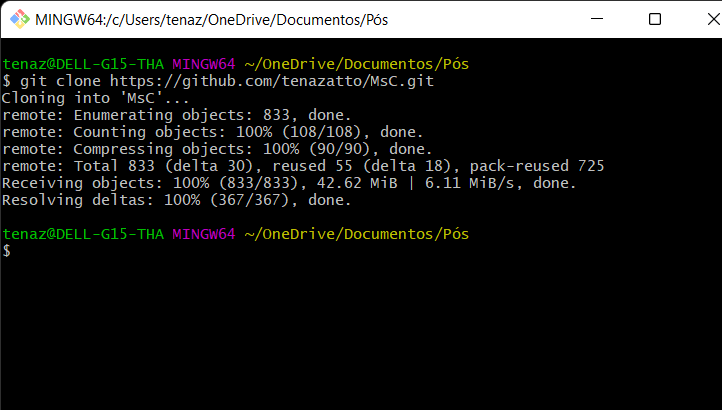
\includegraphics[scale=0.4]{images/doc-install/git-clone.png}
\label{fig:DocInstallGitClone}
\end{figure}

\subsection{Montagem de ambiente}

Para evitar problemas de versão com bibliotecas de outros projetos instalados, é possível criar um ambiente virtual para realizar a instalação das bibliotecas separadamente. Para criar, é necessário o \textbf{virtualenv} instalado no Python. Caso ele não esteja instalado, ele é obtido através do comando:

\begin{quote}\textbf{pip install virtualenv}\end{quote}

Para criar um novo ambiente virtual, é preciso digitar o comando

\begin{quote}\textbf{python3 -m venv ./(nome do ambiente)}\end{quote}

Como exemplo, nesta documentação foi criado o documento \textbf{testenv}

\begin{figure}[H]
\centering
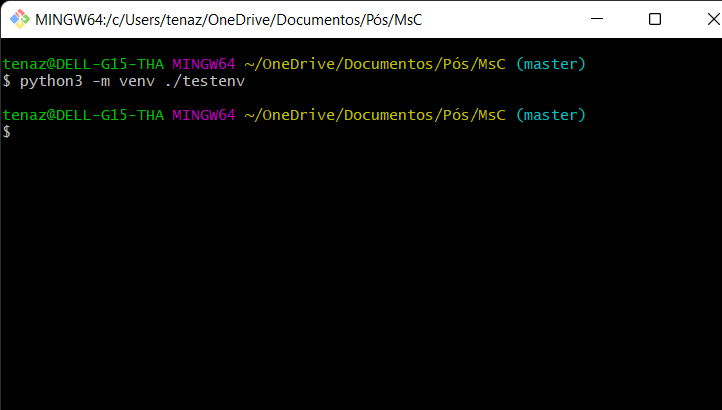
\includegraphics[scale=0.4]{images/doc-install/virtualenv-sh.png}
\label{fig:DocInstallVirtualEnvShell}
\end{figure}

Após o término, aparecerá uma nova pasta de mesmo nome

\begin{figure}[H]
\centering
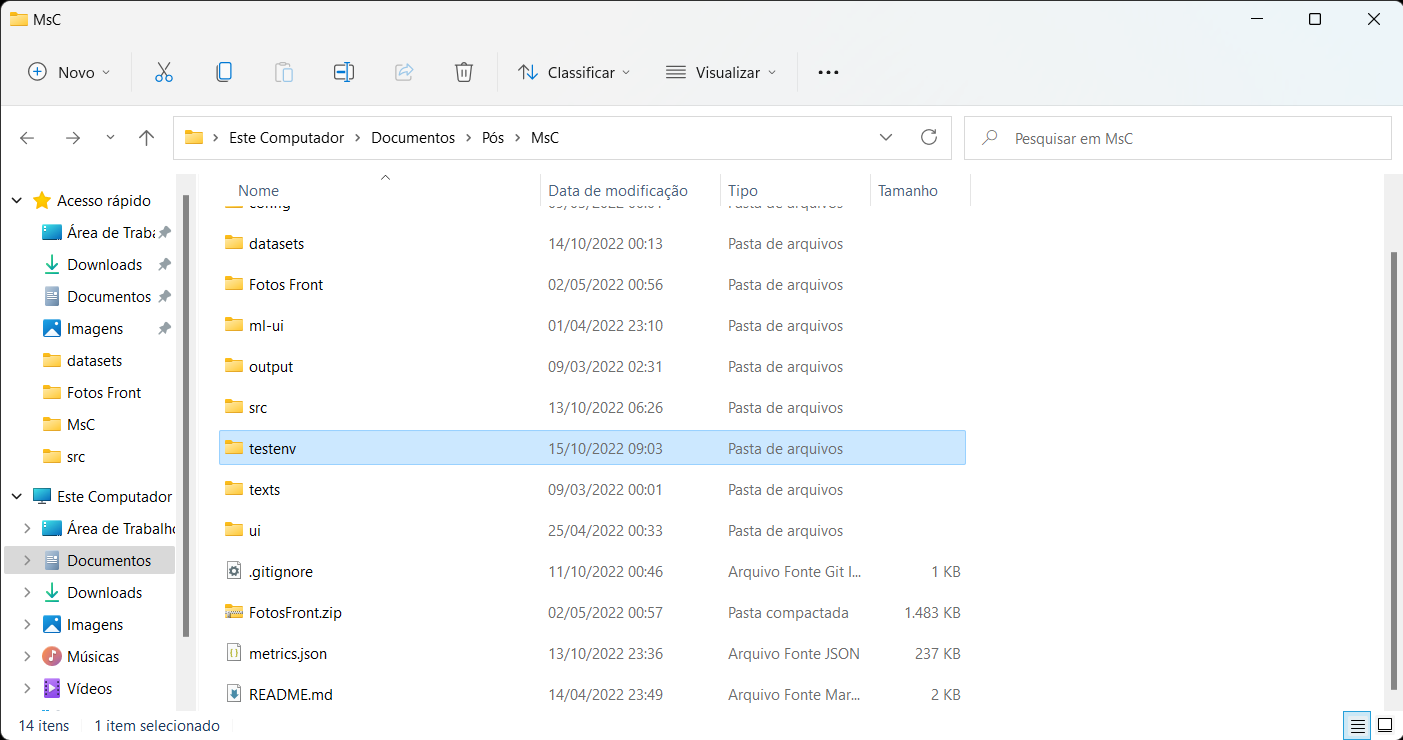
\includegraphics[scale=0.25]{images/doc-install/virtualenv.png}
\label{fig:DocInstallVirtualEnvFolder}
\end{figure}

Após criar o ambiente virtual, é preciso ativá-lo para utilizar

\begin{quote}
\textbf{.\textbackslash (nome do ambiente)\textbackslash Scripts\textbackslash activate.bat} (Windows - Prompt de Comando)
\end{quote}
\begin{quote}
\textbf{source ./(nome do ambiente)/Scripts/activate} (Windows - Bash)
\end{quote}
\begin{quote}
\textbf{source ./(nome do ambiente)/bin/activate} (Linux)
\end{quote}

Para verificar se o ambiente foi ativado, é possível verificar, ao digitar qualquer comando no bash, que o nome do ambiente virtual aparece logo abaixo.

\begin{figure}[h!]
\centering
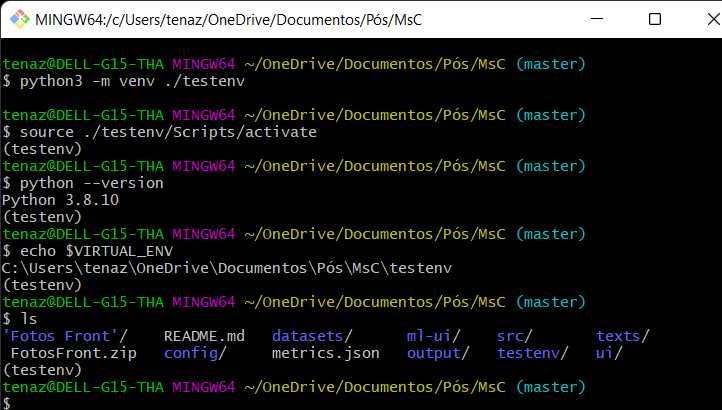
\includegraphics[scale=0.4]{images/doc-install/virtualenv-check.png}
\label{fig:DocInstallVirtualEnvCheck}
\end{figure}

Para desativar o ambiente virtual, é preciso digitar o comando

\begin{quote}\textbf{deactivate}\end{quote}

Para verificar se o ambiente foi desativado, é possível verificar, ao digitar qualquer comando no bash, que o nome do ambiente virtual não irá mais aparecer até ser ativado novamente.

No caso do Node.js não é necessário realizar tais etapas, pois a instalação das bibliotecas nesta documentação é realizada de maneira local

\subsection{Instalação das bibliotecas}

\subsubsection{Python}

Com o ambiente virtual criado e ativado, é possível utilizar os arquivos \textbf{src/requirements.txt}, dependendo das configurações da sua máquina, para instalar todas as bibliotecas necessárias através do comando

\begin{quote}\textbf{pip install -r ./src/requirements-nvidia.txt} (GPU Nvidia)\end{quote}
\begin{quote}\textbf{pip install -r ./src/requirements-cpu.txt} (CPU)\end{quote}

Estes arquivos foram preparados apenas para rodar de acordo com o hardware apresentado. A execução de ambos os comandos não é necessária e nem recomendável.

\subsubsection{Node.js}

Para o Node.js, como o arquivo \textbf{package.json} está dentro da pasta \textbf{ml-ui}, é possível acessar essa pasta e digitar o comando

\begin{quote}\textbf{npm install}\end{quote}

\section{Execução do sistema}

\subsection{Engenharia de dados}

Dentro da pasta \textbf{MsC} e com o ambiente virtual criado e ativado, para rodar a etapa de Engenharia de dados basta digitar o seguinte comando

\begin{quote}\textbf{python -m src.data\_engineering.data\_engineering\_start -{}-data (Opção)}\end{quote}

No momento, há 3 opções disponíveis:

\begin{itemize}
    \item {\textbf{GERMAN\_CREDIT:}} Manipula o German Credit Dataset, cujo arquivo está na localização \textbf{datasets/german.data}, para utilização no Workflow.
    \item {\textbf{LENDINGCLUB:}} Baixa e manipula o Lendingclub Dataset para utilização no Workflow.
    \item {\textbf{METRICS:}} Obtém o maior valor, menor valor e a média de cada métrica para cada Workflow já executado.
\end{itemize}

\subsection{Workflow de IA}

Dentro da pasta \textbf{MsC} e com o ambiente virtual criado e ativado, para rodar todos os Workflows possíveis basta digitar o seguinte comando

\begin{quote}\textbf{python -m src.pipeline.pipeline\_start -{}-dataset (Opção)}\end{quote}

No momento, há 4 opções disponíveis:

\begin{itemize}
    \item {\textbf{ADULT\_INCOME\_SEX:}} Executa os Workflows para o Adult Income Dataset, cujo arquivo está na localização \textbf{datasets/adult.csv}, utilizando Sexo (Masculino/Feminino) como atributo protegido.
    \item {\textbf{GERMAN\_CREDIT\_FOREIGN:}} Executa os Workflows para o German Credit Dataset, cujo arquivo é manipulado na etapa anterior, utilizando Nacionalidade (Alemão/Estrangeiro) como atributo protegido.
    \item {\textbf{GERMAN\_CREDIT\_AGE:}} Executa os Workflows para o German Credit Dataset, cujo arquivo é manipulado na etapa anterior, utilizando Idade (-25 anos/25 ou + anos) como atributo protegido.
    \item {\textbf{LENDINGCLUB\_INCOME:}} Executa os Workflows para o Lendingclub Dataset, cujo arquivo é manipulado na etapa anterior, utilizando Renda (-1 salário mínimo/1 ou + salários mínimos) como atributo protegido.
\end{itemize}

Após a execução, é possível ver a geração das métricas dentro da pasta \textbf{output/metrics}, necessárias para a execução da próxima etapa.

\begin{figure}[H]
\centering
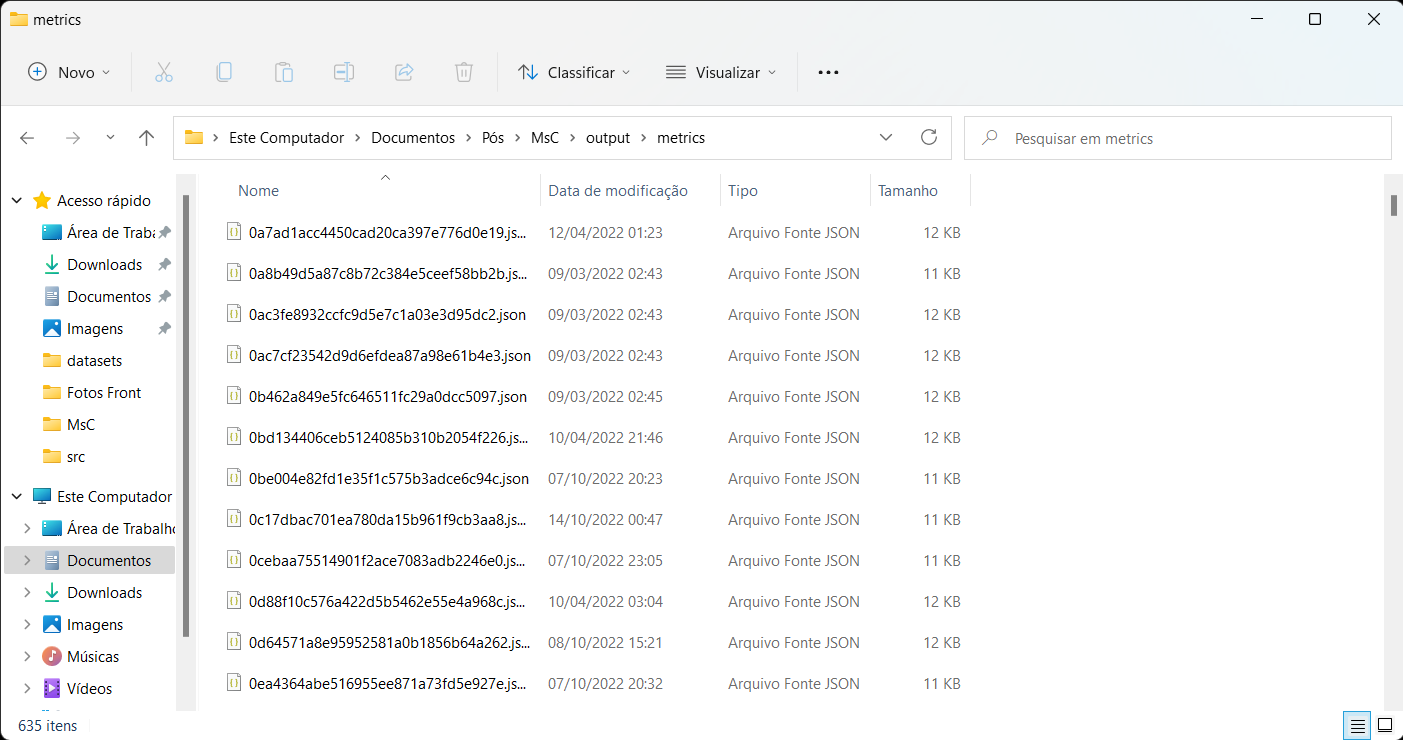
\includegraphics[scale=0.25]{images/doc-install/metrics.png}
\label{fig:DocInstallMetrics}
\end{figure}

\subsection{Autonomia do Workflow}

Dentro da pasta \textbf{MsC}, com o ambiente virtual criado e ativado e com pelo menos um Workflow executado, é possível verificar como a etapa de autonomia funciona com o seguinte comando

\begin{quote}\textbf{python -m src.mapek.mapek\_start}\end{quote}

Nesta etapa, ele escolhe o Workflow que apresentou as melhores métricas, porém a filtragem por conjunto de dados está desenvolvida até o momento apenas na próxima etapa. Como ele roda ininterruptamente, é preciso interromper sua execução.

\subsection{Interface}

\subsubsection{Backend}

Dentro da pasta \textbf{MsC}, com o ambiente virtual criado e ativado e com pelo menos um Workflow executado, é possível rodar o Backend da interface com o seguinte comando

\begin{quote}\textbf{python -m src.api.flask\_start}\end{quote}

Ele vai iniciar um servidor na porta 8080, necessário para rodar as requisições que o Frontend vai solicitar

\begin{figure}[H]
\centering
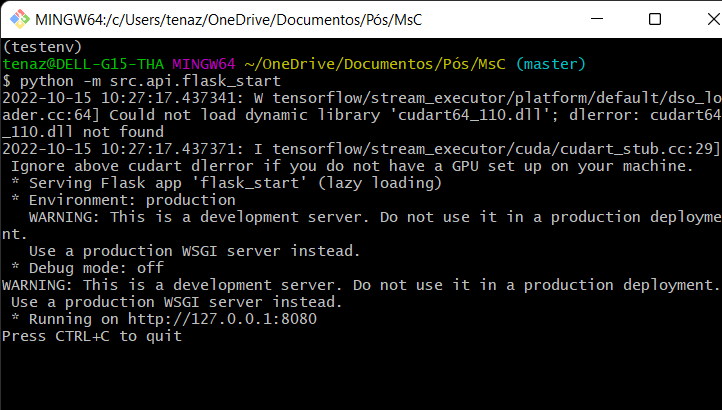
\includegraphics[scale=0.4]{images/doc-install/backend-start.png}
\label{fig:DocInstallVirtualEnvBackendStart}
\end{figure}

\subsubsection{Frontend}

Dentro da pasta \textbf{MsC/ml-ui}, é possível rodar o Frontend da interface com o seguinte comando

\begin{quote}\textbf{npm start}\end{quote}

Ele vai iniciar o navegador acessando um servidor na porta 3000, e deverá iniciar a tela no menu de Análise

\begin{figure}[H]
\centering
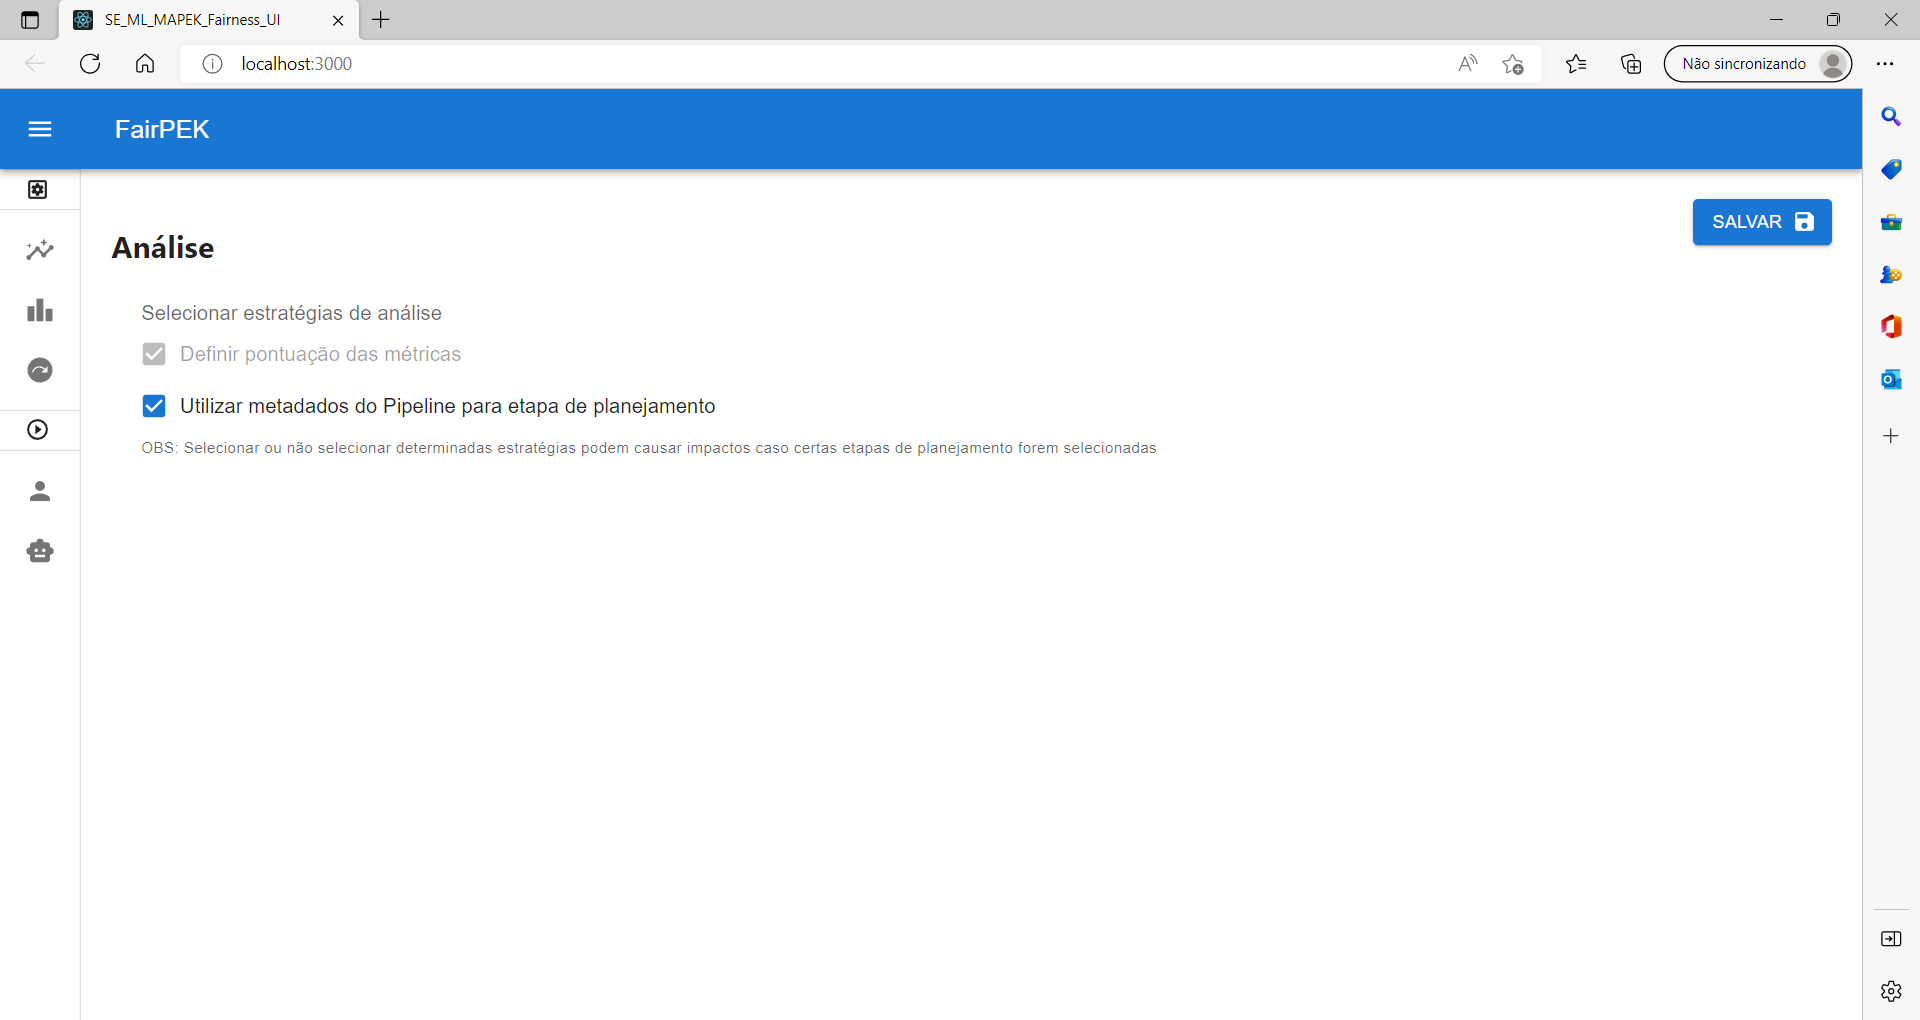
\includegraphics[scale=0.2]{images/doc-install/ml-ui.png}
\label{fig:DocInstallMLUI}
\end{figure}

\chapter{Documentação de Manutenção}
\label{ann:DocMain}

\section{Introdução}

Esta documentação foi criada com o objetivo de guiar o desenvolvedor de Software a entender, configurar e manter este sistema, que é dividido em 4 módulos principais:

\begin{itemize}
    \item {\textbf{Engenharia de dados:}} Etapa criada com o objetivo de simular processos de transformação e limpeza de dados.
    \item {\textbf{Workflow de IA:}} Etapa para execução de um Pipeline que simula o desenvolvimento de uma aplicação automatizada de IA, desde uma categorização dos dados mais específica do que na etapa anterior, passando pelo algoritmo utilizado e finalizando obtendo métricas para determinar qualidade do resultado final.
    \item {\textbf{Autonomia do Workflow (Gerenciador Autonômico):}} Etapa que executa um componente para automatizar todas as etapas do Workflow, com o objetivo de evitar com que perca-se tempo em execuções manuais que podem demorar dependendo do algoritimo e do conjunto de dados utilizado.
    \item {\textbf{Interface:}} Etapa criada com o objetivo de simular a etapa anterior, porém de modo a proporcionar uma experiência de usuário mais simples e intuitiva. É dividida em duas partes:
    \begin{itemize}
        \item {\textbf{Frontend:}} Parte visual, exibida em um navegador.
        \item \textbf{{Backend:}} Parte onde o Frontend se comunica para obter os dados e montar o visual corretamente, de forma que corresponda a configurações utilizadas pelo Gerenciador Autonômico.
    \end{itemize}
\end{itemize}

\section{Arquitetura do Workflow e Framework}

O Workflow usa uma arquitetura chamada de Pipes-and-Filters, onde Pipes, que transportam os dados, são ligados por Filters, que realizam as manipulações desses dados. Pipes e Filters se encadeiam para formar uma sequência de operações, caracterizando todo o Pipeline. Para auxiliar no desenvolvimento, um pequeno framework foi criado, para facilitar as operações necessárias entre Pipes e Filters. 

\subsection{Estrutura}

Pipes herdam a classe \textbf{BasePipe}. Essa classe possui o atributo \textbf{value}, que caracteriza os dados transformados, em formato de um dicionário Python

\begin{lstlisting}[language=Python, label=cod:FairnessPipeClass]
class FairnessPipe(BasePipe):
    privileged\_group = []
    unprivileged_group = []

    label_names = []
    protected_attribute_names = []

    optim_options = {}

    def __init__(self):
        self.value = {
            'privileged_group': self.privileged_group,
            'unprivileged_group': self.unprivileged_group,
            'label_names': self.label_names,
            'protected_attribute_names': self.protected_attribute_names,
            'optim_options': self.optim_options
        }
\end{lstlisting}

Filters herdam a classe \textbf{BaseFilter}. Essa classe possui dois Pipes (input e output) e um método chamado \textbf{execute}, que é onde as operações de transformação do Pipe de input são executadas para serem colocadas no Pipe de output

\begin{lstlisting}[language=Python, label=cod:TrainTestSplitClass]
from sklearn.model_selection import train_test_split

from src.pipeline.pipe_filter.pipe import BaseFilter


class TrainTestSplit(BaseFilter):
    test_size = 0.2

    def __init__(self, test_size=0.2):
        self.test_size = test_size

    def execute(self):
        df_x = self.input['df_x']
        df_y = self.input['df_y']

        x_train, x_test, y_train, y_test = train_test_split(df_x, df_y, test_size=self.test_size, random_state=42)

        self.output = {
            'x_train': x_train,
            'x_test': x_test,
            'y_train': y_train,
            'y_test': y_test,
            'checksum': self.input['checksum']
        }
\end{lstlisting}

\subsection{Operações}

No Framework, estão presentes as seguintes operações:

\subsection{Ligação de Pipe com Filter}

Para juntar um Pipe com um Filter, basta realizar o comando \textbf{>=}, caracterizando o transporte a um Filter.

\begin{lstlisting}[language=Python, label=cod:PipeToFilter]
    Pipe1() >= Filter1()
\end{lstlisting}

Se o Pipe estiver carregando os dados corretos, o Filter será automaticamente executado.

\subsection{Ligação de Filter com Pipe}

Para juntar um Filter com um Pipe, basta realizar o comando \textbf{==}, caracterizando o transporte a um Pipe.

\begin{lstlisting}[language=Python, label=cod:FilterToPipe]
    Filter1() == Pipe1()
\end{lstlisting}

Se o Filter esiver corretamente implementado, o Pipe será caracterizado como a saída desse mesmo Filter.

\subsection{Seleção parcial de dados presentes no Pipe}

Para selecionar apenas alguns atributos presentes no Pipe, basta adicionar colchetes e colocar os campos desejados.

\begin{lstlisting}[language=Python, label=cod:PartialPipe]
    pipe1['campo1', 'campo2', 'campo3']
\end{lstlisting}

\subsection{Junção de Pipes}

Pra juntar os dados de dois pipes em um só, basta realizar o comando \textbf{+}, caracterizando uma junção de Pipes.

\begin{lstlisting}[language=Python, label=cod:MergePipes]
    pipe1 + pipe2
\end{lstlisting}

\section{Incrementos no Workflow}

Aqui estão dois exemplos de como é possível realizar a manuntenção do Workflow

\subsection{Adicionando um novo Conjunto de Dados}

\subsubsection{Engenharia de dados}

\begin{enumerate}
\item Geralmente conjuntos de dados não vem filtrados, e é preciso um trabalho de Engenharia de dados para realizar experimentos com melhores resultados. Neste sistema, a parte de Engenharia de dados se encontra na pasta \textbf{src/data\_engineering}.

\item Os métodos onde os processamentos são realizados ficam no arquivo \textbf{data\_engineering.py}. Para adicionar um novo processamento, basta adicionar um novo método neste arquivo.

\item Importar o novo método no arquivo \textbf{data\_engineering\_start.py}.

\item Adicionar uma nova opção no parâmetro \textbf{choices} presente no método \textbf{parser.add\_argument}

\begin{lstlisting}[language=Python, label=cod:ParserAddArgument]
    parser.add_argument("--data", help="Selecao do gerador do conjunto de dados tratado",
                        choices=['GERMAN_CREDIT', 'LENDINGCLUB', 'METRICS'])
\end{lstlisting}

\item Adicionar uma nova condição com a opção adicionada
\end{enumerate}

\subsubsection{Workflow}

\begin{enumerate}
\item Neste sistema, a parte do Workflow se encontra na pasta \textbf{src/pipeline}. Dentro dela, os Pipes que armazenam os conjuntos de dados se encontram na pasta \textbf{processors/preprocessors/data}. Dentro dela, no arquivo \textbf{dataset.py}, criar uma classe que herda a classe \textbf{Dataset}, preenchendo os atributos \textbf{dataset\_path} com o caminho do arquivo.

\begin{lstlisting}[language=Python, label=cod:FairnessPipe]
class LendingclubDataset(Dataset):
    dataset_path = 'datasets/lendingclub_dataset.csv'

    def __init__(self):
        super().__init__()
\end{lstlisting}

\item Criar um novo arquivo.

\item Criar uma classe que herda a classe \textbf{FairnessPipe}, preenchendo os atributos \textbf{privileged\_group}, \textbf{unprivileged\_group}, \textbf{label\_names}, \textbf{protected\_attribute\_names} e \textbf{optim\_options}.

\begin{lstlisting}[language=Python, label=cod:FairnessPipe]
class LendingclubIncomeFairnessPipe(FairnessPipe):
    privileged_group = [{'annual_inc': 1}]
    unprivileged_group = [{'annual_inc': 0}]

    label_names = ['loan_status']
    protected_attribute_names = ['annual_inc']

    optim_options = {
        "distortion_fun": get_distortion_german,
        "epsilon": 0.05,
        "clist": [0.99, 1.99, 2.99],
        "dlist": [.1, 0.05, 0]
    }

    def __init__(self):
        super().__init__()
\end{lstlisting}

\item Criar uma classe que herda a classe \textbf{FairnessPreprocessor}, preenchendo o método \textbf{dataset\_preprocess} e retornando um DataFrame Pandas de dados de entrada e um DataFrame de dados de saída.

\begin{lstlisting}[language=Python, label=cod:FairnessPreprocessor]
class LendingclubIncomePreprocessor(FairnessPreprocessor):
    def dataset_preprocess(self, df):
        df.info()

        SAMPLE_PERCENTAGE = 100
        df_sample_nok = df[df['loan_status'] == 'Charged Off'].sample(frac=SAMPLE_PERCENTAGE/100)
        df_sample_ok = df[df['loan_status'] == 'Fully Paid'].sample(frac=SAMPLE_PERCENTAGE / 100)
        df_sample = pd.concat([df_sample_ok, df_sample_nok])

        df_x = df_sample.drop('loan_status', axis=1)
        df_y = pd.DataFrame(df_sample.loan_status)

        return df_x, df_y
\end{lstlisting}

\item Na pasta \textbf{src/pipeline/processors} e dentro do arquivo \textbf{enums.py}, colocar novas opções nas classes \textbf{Datasets} e \textbf{Preprocessors}.

\begin{lstlisting}[language=Python, label=cod:EnumOptions]
class Datasets(ExtendedEnum):
    ADULT_INCOME = 1
    GERMAN_CREDIT = 2
    LENDINGCLUB = 3


class Preprocessors(ExtendedEnum):
    SEX = 1
    AGE = 2
    FOREIGN = 3
    INCOME = 4
\end{lstlisting}

\item Na pasta \textbf{src/pipeline} e dentro do arquivo \textbf{validation.py}, atualizar a variável \textbf{existant\_preprocessors} com as novas opções colocadas no item anterior.

\begin{lstlisting}[language=Python, label=cod:ValidationPreprocessors]
        existant_preprocessors = \
            (dataset == Datasets.ADULT_INCOME and preprocessor == Preprocessors.SEX) or \
            (dataset == Datasets.GERMAN_CREDIT and preprocessor == Preprocessors.AGE) or \
            (dataset == Datasets.GERMAN_CREDIT and preprocessor == Preprocessors.FOREIGN) or \
            (dataset == Datasets.LENDINGCLUB and preprocessor == Preprocessors.INCOME)
\end{lstlisting}

\item Na pasta \textbf{src/pipeline} e dentro do arquivo \textbf{pipeline.py}, encontrar o método \textbf{select\_data\_preprocessor}, atualizar a variável \textbf{options} com as novas opções e classes implementadas nos itens anteriores.

\begin{lstlisting}[language=Python, label=cod:PipelinePreprocessors]
    def select_data_preprocessor(self, dataset, preprocessor):
        choice = [dataset, preprocessor]
        options = [
            ([Datasets.ADULT_INCOME, Preprocessors.SEX], (AdultDataset(), AdultSexPreprocessor(), AdultSexFairnessPipe())),
            ([Datasets.GERMAN_CREDIT, Preprocessors.AGE], (GermanDataset(), GermanAgePreprocessor(), GermanAgeFairnessPipe())),
            ([Datasets.GERMAN_CREDIT, Preprocessors.FOREIGN], (GermanDataset(), GermanForeignPreprocessor(), GermanForeignFairnessPipe())),
            ([Datasets.LENDINGCLUB, Preprocessors.INCOME], (LendingclubDataset(), LendingclubIncomePreprocessor(), LendingclubIncomeFairnessPipe())),
        ]

        for option, pipe_filter in options:
            if choice == option:
                dataset_pipe, data_preprocessor_filter, fairness_pipe = pipe_filter
                preprocessed_data_pipe = dataset_pipe >= data_preprocessor_filter == self.new_pipe()
                break

        return preprocessed_data_pipe, fairness_pipe
\end{lstlisting}

\item Na pasta \textbf{src/pipeline} e dentro do arquivo \textbf{pipeline\_start.py}, adicionar uma nova opção no parâmetro \textbf{choices} presente no método \textbf{parser.add\_argument}.

\begin{lstlisting}[language=Python, label=cod:ParserAddArgumentPipeline]
    parser.add_argument("--dataset", help="Conjunto de dados tratado com atributo protegido",
                        choices=['ADULT_INCOME_SEX',
                                 'GERMAN_CREDIT_FOREIGN', 'GERMAN_CREDIT_AGE',
                                 'LENDINGCLUB_INCOME'])
\end{lstlisting}

\item No mesmo arquivo, adicionar uma nova condição com a opção adicionada.

\begin{lstlisting}[language=Python, label=cod:IfPipelineStart]
    if args.dataset == 'ADULT_INCOME_SEX':
        datasets.append((Datasets.ADULT_INCOME, Preprocessors.SEX))
    elif args.dataset == 'ADULT_INCOME_FOREIGN':
        datasets.append((Datasets.GERMAN_CREDIT, Preprocessors.FOREIGN))
    elif args.dataset == 'GERMAN_CREDIT_AGE':
        datasets.append((Datasets.GERMAN_CREDIT, Preprocessors.AGE))
    elif args.dataset == 'LENDINGCLUB_INCOME':
        datasets.append((Datasets.LENDINGCLUB, Preprocessors.INCOME))]
\end{lstlisting}

\end{enumerate}

\subsubsection{Interface (Backend)}

\begin{enumerate}
\item Neste sistema, a parte do Backend se encontra na pasta \textbf{src/api}. Dentro dela, no arquivo \textbf{repo/pipeline.py}, adicionar a opção no método \textbf{get\_dataset}.

\begin{lstlisting}[language=Python, label=cod:AddDataset]
    def get_dataset(self, dataset):
        indexes = {
            'Datasets.ADULT_INCOME': Datasets.ADULT_INCOME,
            'Datasets.GERMAN_CREDIT': Datasets.GERMAN_CREDIT,
            'Datasets.LENDINGCLUB': Datasets.LENDINGCLUB,
        }

        return next(filter(lambda a: a[0] == dataset, indexes.items()))[1]
\end{lstlisting}

\item Na pasta \textbf{src/api} e dentro do arquivo \textbf{repo/pipeline.py}, adicionar a opção no método \textbf{get\_preprocessor}.

\begin{lstlisting}[language=Python, label=cod:AddDataset]
    def get_preprocessor(self, preprocessor):
        indexes = {
            'Preprocessors.SEX': Preprocessors.SEX,
            'Preprocessors.AGE': Preprocessors.AGE,
            'Preprocessors.FOREIGN': Preprocessors.FOREIGN
        }

        return next(filter(lambda a: a[0] == preprocessor, indexes.items()))[1]
\end{lstlisting}
\end{enumerate}

\subsubsection{Interface (Frontend)}

\begin{enumerate}
\item Neste sistema, a parte do Frontend se encontra na pasta \textbf{ml-ui/src}. Dentro dela, no arquivo \textbf{Auto-Pipeline-Menu.js}, adicionar a opção colocada na etapa de Workflow no componente Select onde estão as outras opções de conjunto de dados.

\begin{lstlisting}[language=Python, label=cod:AddDatasetAuto]
<Select
  sx={{fontSize: '14px'}}
  value={dataset}
  onChange={handleDatasetChange}
  displayEmpty
  inputProps={{ 'aria-label': 'Without label' }}
>
  <MenuItem value={'Datasets.ADULT_INCOME'}>Adult Income Dataset</MenuItem>
  <MenuItem value={'Datasets.GERMAN_CREDIT'}>German Credit Dataset</MenuItem>
  <MenuItem value={'Datasets.LENDINGCLUB'}>Lendingclub Dataset</MenuItem>
</Select>
\end{lstlisting}

\item Na pasta \textbf{ml-ui/src} e dentro do arquivo \textbf{Manual-Pipeline-Menu.js}, adicionar a opção colocada na etapa de Workflow no componente Select onde estão as outras opções de conjunto de dados.

\begin{lstlisting}[language=Python, label=cod:AddDatasetManual]
<Select
  sx={{fontSize: '14px'}}
  value={dataset}
  onChange={handleDatasetChange}
  displayEmpty
  inputProps={{ 'aria-label': 'Without label' }}
>
  <MenuItem value={'Datasets.ADULT_INCOME'}>Adult Income Dataset</MenuItem>
  <MenuItem value={'Datasets.GERMAN_CREDIT'}>German Credit Dataset</MenuItem>
  <MenuItem value={'Datasets.LENDINGCLUB'}>Lendingclub Dataset</MenuItem>
</Select>
\end{lstlisting}

\item Na pasta \textbf{ml-ui/src} e dentro do arquivo \textbf{Manual-Pipeline-Menu.js}, adicionar a opção colocada na etapa de Workflow no componente Select onde estão as outras opções de pré-processadores.

\begin{lstlisting}[language=Python, label=cod:AddDatasetManual]
<FormControl sx={{ m: 1, width: 300, marginLeft: '35px' }}>
  {dataset === 'Datasets.ADULT_INCOME' ?
    <Select
      sx={{fontSize: '14px'}}
      value={protectedAtt}
      onChange={handleProtectedAttChange}
      displayEmpty
      inputProps={{ 'aria-label': 'Without label' }}
    >
      <MenuItem value={'Preprocessors.SEX'}>Sexo (Masculino/Feminino)</MenuItem>
    </Select>
  : dataset === 'Datasets.ADULT_INCOME' ?
    <Select
      sx={{fontSize: '14px'}}
      value={protectedAtt}
      onChange={handleProtectedAttChange}
      displayEmpty
      inputProps={{ 'aria-label': 'Without label' }}
    >
      <MenuItem value={'Preprocessors.AGE'}>Idade (-25 anos/+25 anos)</MenuItem>
      <MenuItem value={'Preprocessors.FOREIGN'}>Nacionalidade (Local/Estrangeiro)</MenuItem>
    </Select>
  :
    <Select
      sx={{fontSize: '14px'}}
      value={protectedAtt}
      onChange={handleProtectedAttChange}
      displayEmpty
      inputProps={{ 'aria-label': 'Without label' }}
    >
      <MenuItem value={'Preprocessors.INCOME'}>Renda (-1 Salario Minimo/1+ Salarios Minimos)</MenuItem>
    </Select>
  }
  <FormHelperText>Atributo protegido para medir justica</FormHelperText>
</FormControl>
\end{lstlisting}

\item Na pasta \textbf{ml-ui/src} e dentro do arquivo \textbf{Manual-Pipeline-Menu.js} adicionar a condição para a opção colocada na etapa de Workflow no método \textbf{handleDatasetChange}.

\begin{lstlisting}[language=Python, label=cod:AddDatasetManual]
  const handleDatasetChange = (event) => {
    setDataset(event.target.value);

    if (event.target.value === 'Datasets.ADULT_INCOME') {
      setProtectedAtt('Preprocessors.SEX');
    } else if (event.target.value === 'Datasets.GERMAN_CREDIT') {
      setProtectedAtt('Preprocessors.AGE');
    } else {
      setProtectedAtt('Preprocessors.INCOME');
    }
  }
\end{lstlisting}
\end{enumerate}

\subsection{Adicionando um novo Algoritmo}

\subsubsection{Workflow}

\begin{enumerate}
\item Neste sistema, a parte do Workflow se encontra na pasta \textbf{src/pipeline}. Dentro dela, os Filters que executam os algoritmos ficam dentro da pasta \textbf{processors}. Dentro dela, no arquivo \textbf{enums.py}, colocar novas opções na classe \textbf{Algorithms}.

\begin{lstlisting}[language=Python, label=cod:EnumAlgorithmOptions]
class Algorithms:
    LOGISTIC_REGRESSION = 1
    RANDOM_FOREST = 2
    GRADIENT_BOOST = 3
    SUPPORT_VECTOR_MACHINES = 4
    LINEAR_REGRESSION = 901
    DECISION_TREE = 902
    KERNEL_RIDGE = 903
\end{lstlisting}

A classe \textbf{Algorithms} serve para este exemplo em questão, mas para outros tipos de algoritmos as classes \textbf{UnbiasDataAlgorithms}, \textbf{UnbiasInProcAlgorithms} ou \textbf{UnbiasPostProcAlgorithms} podem ser mais adequadas.

\item Na pasta \textbf{src/pipeline} e dentro do arquivo \textbf{validation.py}, adicionar uma nova condição para a variável \textbf{existant\_algorithms} no método \textbf{validate\_params}.

\begin{lstlisting}[language=Python, label=cod:ValidationAddArgumentPipeline]
            existant_algorithms = \
            (algorithm == Algorithms.LOGISTIC_REGRESSION and unbias_data_algorithm == UnbiasDataAlgorithms.NOTHING and unbias_postproc_algorithm == UnbiasPostProcAlgorithms.NOTHING) or \
            (...)
            (algorithm == UnbiasInProcAlgorithms.GRID_SEARCH_REDUCTION and unbias_data_algorithm == UnbiasDataAlgorithms.NOTHING and unbias_postproc_algorithm == UnbiasPostProcAlgorithms.NOTHING) or \
            (algorithm == Algorithms.NOVA_OPCAO and unbias_data_algorithm == UnbiasDataAlgorithms.NOTHING and unbias_postproc_algorithm == UnbiasPostProcAlgorithms.NOTHING) or \
            (algorithm == Algorithms.NOVA_OPCAO and unbias_data_algorithm == UnbiasDataAlgorithms.NOTHING and unbias_postproc_algorithm == UnbiasPostProcAlgorithms.EQUALIZED_ODDS) or \
            (algorithm == Algorithms.NOVA_OPCAO and unbias_data_algorithm == UnbiasDataAlgorithms.NOTHING and unbias_postproc_algorithm == UnbiasPostProcAlgorithms.CALIBRATED_EQUALIZED_ODDS) or \
            (algorithm == Algorithms.NOVA_OPCAO and unbias_data_algorithm == UnbiasDataAlgorithms.NOTHING and unbias_postproc_algorithm == UnbiasPostProcAlgorithms.REJECT_OPTION_CLASSIFICATION) or \
            (algorithm == Algorithms.NOVA_OPCAO and unbias_data_algorithm == UnbiasDataAlgorithms.REWEIGHING and unbias_postproc_algorithm == UnbiasPostProcAlgorithms.NOTHING) or \
            (algorithm == Algorithms.NOVA_OPCAO and unbias_data_algorithm == UnbiasDataAlgorithms.DISPARATE_IMPACT_REMOVER and unbias_postproc_algorithm == UnbiasPostProcAlgorithms.NOTHING) or \
            (algorithm == Algorithms.NOVA_OPCAO and unbias_data_algorithm == UnbiasDataAlgorithms.OPTIMIZED_PREPROCESSING and unbias_postproc_algorithm == UnbiasPostProcAlgorithms.NOTHING) or \
            (algorithm == Algorithms.NOVA_OPCAO and unbias_data_algorithm == UnbiasDataAlgorithms.LEARNING_FAIR_REPRESENTATIONS and unbias_postproc_algorithm == UnbiasPostProcAlgorithms.NOTHING)
\end{lstlisting}

\item Na pasta \textbf{src/pipeline} e dentro do arquivo \textbf{pipeline.py}, colocar as novas opções colocadas no item anterior no método \textbf{find\_algorithm}.

\begin{lstlisting}[language=Python, label=cod:FindAlgorithm]
    def find_algorithm(self, algorithm):
        indexes = {
            'Algorithms.LOGISTIC_REGRESSION': 1,
            'Algorithms.RANDOM_FOREST': 2,
            'Algorithms.GRADIENT_BOOST': 3,
            'Algorithms.SUPPORT_VECTOR_MACHINES': 4,
            'Algorithms.LINEAR_REGRESSION': 901,
            'Algorithms.DECISION_TREE': 902,
            'Algorithms.KERNEL_RIDGE': 903,
            'UnbiasInProcAlgorithms.PREJUDICE_REMOVER': 101,
            'UnbiasInProcAlgorithms.ADVERSARIAL_DEBIASING': 102,
            'UnbiasInProcAlgorithms.EXPONENTIATED_GRADIENT_REDUCTION': 103,
            'UnbiasInProcAlgorithms.RICH_SUBGROUP_FAIRNESS': 104,
            'UnbiasInProcAlgorithms.GRID_SEARCH_REDUCTION': 105,
            'UnbiasInProcAlgorithms.META_FAIR_CLASSIFIER': 106,
            'UnbiasInProcAlgorithms.ART_CLASSIFIER': 107
        }

        return next(filter(lambda a: a[1] == algorithm, indexes.items()))[0]
\end{lstlisting}

\item Criar um novo arquivo na pasta categorizada pelo algoritmo a ser implementado. Para o exemplo exemplo ilustrado abaixo, como o Gradient Boosting é um algoritmo de treinamento e não foi projetado para redução de viés, os Filters que executam os algoritmos se encontram na pasta \textbf{processors/inprocessors/inproc\_algorithms}.

Seguem as pastas onde os respectivos Filters se encontram:

\begin{itemize}
\item \textbf{Algoritmo de treinamento sem redução de viés:} processors/inprocessors/inproc\_algorithms
\item \textbf{Algoritmo com redução de viés no dado (Pré-processamento):} processors/preprocessors/unbias\_algorithms
\item \textbf{Algoritmo com redução de viés no treinamento (Processamento):} processors/inprocessors/unbias\_algorithms
\item \textbf{Algoritmo com redução de viés no resultado (Pós-processamento):} processors/postprocessors
\end{itemize}

\item No arquivo criado, criar uma classe que herda a classe \textbf{BaseFilter}.

\begin{lstlisting}[language=Python, label=cod:BaseFilter]
class GradientBoostFilter(BaseFilter):
    weighed = False

    def __init__(self, weighed=False):
        self.weighed = weighed
\end{lstlisting}

\item Implementar nesta classe o método \textbf{execute}, atribuindo em \textbf{self.output} um dicionário Python com os atributos \textbf{y\_pred} e \textbf{scores}.

\begin{lstlisting}[language=Python, label=cod:FilterExecute]
    def execute(self):
        y_pred, scores = self.gradient_boost_weighed() if self.weighed else self.gradient_boost()

        self.output = {
            'y_pred': y_pred,
            'scores': scores
        }
\end{lstlisting}

\item Na pasta \textbf{src/pipeline} e dentro do arquivo \textbf{pipeline.py}, encontrar o método \textbf{process}, atualizar a variável \textbf{process\_options} com as novas opções e classes implementadas nos itens anteriores.

\begin{lstlisting}[language=Python, label=cod:ProcessAlgorithm]
    def process(self, process_pipe, algorithm, unbias_data_algorithm):
        weighed_algorithm = unbias_data_algorithm == UnbiasDataAlgorithms.REWEIGHING or \
                            unbias_data_algorithm == UnbiasDataAlgorithms.LEARNING_FAIR_REPRESENTATIONS

        process_options = [
            (Algorithms.LOGISTIC_REGRESSION, LogisticRegressionFilter(weighed=weighed_algorithm)),
            (Algorithms.RANDOM_FOREST, RandomForestFilter(weighed=weighed_algorithm)),
            (Algorithms.GRADIENT_BOOST, GradientBoostFilter(weighed=weighed_algorithm)),
            (Algorithms.SUPPORT_VECTOR_MACHINES, SVMFilter(weighed=weighed_algorithm)),
            (UnbiasInProcAlgorithms.PREJUDICE_REMOVER, PrejudiceRemoverFilter()),
            (UnbiasInProcAlgorithms.ADVERSARIAL_DEBIASING, AdversarialDebiasingFilter()),
            (UnbiasInProcAlgorithms.EXPONENTIATED_GRADIENT_REDUCTION, ExponentiatedGradientReductionFilter(algorithm=Algorithms.GRADIENT_BOOST)),
            (UnbiasInProcAlgorithms.RICH_SUBGROUP_FAIRNESS, RichSubgroupFairnessFilter(algorithm=Algorithms.DECISION_TREE)),
            (UnbiasInProcAlgorithms.META_FAIR_CLASSIFIER, MetaFairClassifierFilter()),
            (UnbiasInProcAlgorithms.GRID_SEARCH_REDUCTION, GridSearchReductionFilter(algorithm=Algorithms.RANDOM_FOREST))
        ]

        for option, filter in process_options:
            if algorithm == option:
                prediction_pipe = process_pipe >= filter == self.new_pipe()
                break

        return prediction_pipe
\end{lstlisting}

O método \textbf{process} serve para este exemplo em questão, mas para outros tipos de algoritmos os métodos \textbf{unbias\_data\_preprocessor} ou \textbf{data\_postprocess} podem ser mais adequados.

\item Na pasta \textbf{src/pipeline} dentro do arquivo \textbf{pipeline\_start.py}, adicionar as opções (adaptadas a opção corrente) na variável \textbf{process\_options}.

\begin{lstlisting}[language=Python, label=cod:ParserAddArgumentPipeline]
    process_options = [
        (Algorithms.NOVA_OPCAO, UnbiasDataAlgorithms.NOTHING, UnbiasPostProcAlgorithms.NOTHING),
        (Algorithms.NOVA_OPCAO, UnbiasDataAlgorithms.NOTHING, UnbiasPostProcAlgorithms.EQUALIZED_ODDS),
        (Algorithms.NOVA_OPCAO, UnbiasDataAlgorithms.NOTHING,
         UnbiasPostProcAlgorithms.CALIBRATED_EQUALIZED_ODDS),
        (Algorithms.NOVA_OPCAO, UnbiasDataAlgorithms.NOTHING,
         UnbiasPostProcAlgorithms.REJECT_OPTION_CLASSIFICATION),
        (Algorithms.NOVA_OPCAO, UnbiasDataAlgorithms.REWEIGHING, UnbiasPostProcAlgorithms.NOTHING),
        (Algorithms.NOVA_OPCAO, UnbiasDataAlgorithms.DISPARATE_IMPACT_REMOVER,
         UnbiasPostProcAlgorithms.NOTHING),
        # (Algorithms.NOVA_OPCAO, UnbiasDataAlgorithms.OPTIMIZED_PREPROCESSING, UnbiasPostProcAlgorithms.NOTHING),
        (Algorithms.NOVA_OPCAO, UnbiasDataAlgorithms.LEARNING_FAIR_REPRESENTATIONS,
         UnbiasPostProcAlgorithms.NOTHING)
    ]
\end{lstlisting}

\end{enumerate}

\subsubsection{MAPE-K}

\begin{enumerate}
\item Neste sistema, a parte do Backend se encontra na pasta \textbf{src/mapek}. Dentro dela, no arquivo \textbf{ml/planner.py}, colocar as novas opções colocadas no item anterior no método \textbf{find\_inproc\_algorithm}.

\begin{lstlisting}[language=Python, label=cod:findInprocAlgorithm]
    def find_inproc_algorithm(self, algorithm):
        indexes = {
            'Algorithms.LOGISTIC_REGRESSION': 1,
            'Algorithms.RANDOM_FOREST': 2,
            'Algorithms.GRADIENT_BOOST': 3,
            'Algorithms.SUPPORT_VECTOR_MACHINES': 4,
            'Algorithms.LINEAR_REGRESSION': 901,
            'Algorithms.DECISION_TREE': 902,
            'Algorithms.KERNEL_RIDGE': 903,
            'UnbiasInProcAlgorithms.PREJUDICE_REMOVER': 101,
            'UnbiasInProcAlgorithms.ADVERSARIAL_DEBIASING': 102,
            'UnbiasInProcAlgorithms.EXPONENTIATED_GRADIENT_REDUCTION': 103,
            'UnbiasInProcAlgorithms.RICH_SUBGROUP_FAIRNESS': 104,
            'UnbiasInProcAlgorithms.GRID_SEARCH_REDUCTION': 105,
            'UnbiasInProcAlgorithms.META_FAIR_CLASSIFIER': 106,
            'UnbiasInProcAlgorithms.ART_CLASSIFIER': 107
        }

        return next(filter(lambda a: a[0] == algorithm, indexes.items()))[1]
\end{lstlisting}
\end{enumerate}

\subsubsection{Interface (Backend)}

\begin{enumerate}
\item Neste sistema, a parte do Backend se encontra na pasta \textbf{src/api}. Dentro dela, no arquivo \textbf{repo/pipeline.py}, colocar as novas opções colocadas no item anterior no método \textbf{get\_inproc\_algorithm}.

\begin{lstlisting}[language=Python, label=cod:getInprocAlgorithm]
    def get_inproc_algorithm(self, algorithm):
        indexes = {
            'Algorithms.LOGISTIC_REGRESSION': 1,
            'Algorithms.RANDOM_FOREST': 2,
            'Algorithms.GRADIENT_BOOST': 3,
            'Algorithms.SUPPORT_VECTOR_MACHINES': 4,
            'Algorithms.LINEAR_REGRESSION': 901,
            'Algorithms.DECISION_TREE': 902,
            'Algorithms.KERNEL_RIDGE': 903,
            'UnbiasInProcAlgorithms.PREJUDICE_REMOVER': 101,
            'UnbiasInProcAlgorithms.ADVERSARIAL_DEBIASING': 102,
            'UnbiasInProcAlgorithms.EXPONENTIATED_GRADIENT_REDUCTION': 103,
            'UnbiasInProcAlgorithms.RICH_SUBGROUP_FAIRNESS': 104,
            'UnbiasInProcAlgorithms.GRID_SEARCH_REDUCTION': 105,
            'UnbiasInProcAlgorithms.META_FAIR_CLASSIFIER': 106,
            'UnbiasInProcAlgorithms.ART_CLASSIFIER': 107
        }

        return next(filter(lambda a: a[0] == algorithm, indexes.items()))[1]
\end{lstlisting}
\end{enumerate}

\subsubsection{Interface (Frontend)}

\begin{enumerate}
\item Neste sistema, a parte do Frontend se encontra na pasta \textbf{ml-ui/src}. Dentro dela, no arquivo \textbf{Manual-Pipeline-Menu.js}, adicionar a opção colocada na etapa de Workflow no componente Select onde estão as outras opções de algoritmos.

\begin{lstlisting}[language=Python, label=cod:AddAlgorithmManual]
<Select
  sx={{fontSize: '14px'}}
  value={trainAlgorithm}
  onChange={handleTrainAlgorithmChange}
  displayEmpty
  inputProps={{ 'aria-label': 'Without label' }}
>
  <MenuItem value={'Algorithms.LOGISTIC_REGRESSION'}>Logistic Regression</MenuItem>
  <MenuItem value={'Algorithms.RANDOM_FOREST'}>Random Forest</MenuItem>
  <MenuItem value={'Algorithms.GRADIENT_BOOST'}>Gradient Boost</MenuItem>
  <MenuItem value={'Algorithms.SUPPORT_VECTOR_MACHINES'}>Support Vector Machines</MenuItem>
</Select>
\end{lstlisting}

\item Na pasta \textbf{ml-ui/src} e dentro do arquivo \textbf{Planning-Menu.js}, adicionar as opções (adaptadas a opção corrente) na variável \textbf{validAlgorithms}.
\end{enumerate}

\begin{lstlisting}[language=Python, label=cod:AddPlanningConfig]
    {
      options: ["Algorithms.NOVA_OPCAO", "UnbiasDataAlgorithms.NOTHING", "UnbiasPostProcAlgorithms.NOTHING"],
      labels: ["Nome da nova opcao", "Sem metodo", "Sem metodo"],
      selected: true
    },
    {
      options: ["Algorithms.NOVA_OPCAO", "UnbiasDataAlgorithms.NOTHING", "UnbiasPostProcAlgorithms.EQUALIZED_ODDS"],
      labels: ["Nome da nova opcao", "Sem metodo", "Equalized Odds"],
      selected: true
    },
    {
      options: ["Algorithms.NOVA_OPCAO", "UnbiasDataAlgorithms.NOTHING", "UnbiasPostProcAlgorithms.CALIBRATED_EQUALIZED_ODDS"],
      labels: ["Nome da nova opcao", "Sem metodo", "Calibrated Equalized Odds"],
      selected: true
    },
    {
      options: ["Algorithms.NOVA_OPCAO", "UnbiasDataAlgorithms.NOTHING", "UnbiasPostProcAlgorithms.REJECT_OPTION_CLASSIFICATION"],
      labels: ["Nome da nova opcao", "Sem metodo", "Reject Option Classification"],
      selected: true
    },
    {
      options: ["Algorithms.NOVA_OPCAO", "UnbiasDataAlgorithms.REWEIGHING", "UnbiasPostProcAlgorithms.NOTHING"],
      labels: ["Nome da nova opcao", "Reweighing", "Sem metodo"],
      selected: true
    },
    {
      options: ["Algorithms.NOVA_OPCAO", "UnbiasDataAlgorithms.DISPARATE_IMPACT_REMOVER", "UnbiasPostProcAlgorithms.NOTHING"],
      labels: ["Nome da nova opcao", "Disparate Impact Remover", "Sem metodo"],
      selected: true
    },
    {
      options: ["Algorithms.NOVA_OPCAO", "UnbiasDataAlgorithms.OPTIMIZED_PREPROCESSING", "UnbiasPostProcAlgorithms.NOTHING"],
      labels: ["Nome da nova opcao", "Optimized Preprocessing", "Sem metodo"],
      selected: true
    },
    {
      options: ["Algorithms.NOVA_OPCAO", "UnbiasDataAlgorithms.LEARNING_FAIR_REPRESENTATIONS", "UnbiasPostProcAlgorithms.NOTHING"],
      labels: ["Nome da nova opcao", "Learning Fair Representations", "Sem metodo"],
      selected: true
    }
\end{lstlisting}

\chapter{Questionário Aplicado ao Desenvolvedor}
\label{ann:Questionary}

\textbf{Observação:} Nome e e-mail não disponibilizados para manter o anonimato.
\linebreak
\linebreak
\fbox{\begin{minipage}{38em}
\textbf{Nome:} ************

\textbf{E-mail:} *******************

\textbf{Anos de experiência em Desenvolvimento de Aplicações:}

\begin{itemize}
\item[\Square] Não tive experiência
\item[\Square] Até 2 Anos
\item[\Square] 2 a 5 Anos
\item[\XBox] Mais de 5 Anos
\end{itemize}

\textbf{Anos de experiência em Engenharia de Dados:} 

\begin{itemize}
\item[\Square] Não tive experiência
\item[\XBox] Até 2 Anos
\item[\Square] 2 a 5 Anos
\item[\Square] Mais de 5 Anos
\end{itemize}

\textbf{Anos de experiência em Ciência de Dados:} 

\begin{itemize}
\item[\Square] Não tive experiência
\item[\XBox] Até 2 Anos
\item[\Square] 2 a 5 Anos
\item[\Square] Mais de 5 Anos
\end{itemize}
\vskip 1cm
\end{minipage}}

\noindent
\fbox{\begin{minipage}{38em}
\textbf{Quais os pontos positivos ao realizar o desenvolvimento?}

A documentação possui informações detalhadas sobre o que é e como funciona o Framework, explicando as tecnologias usadas, como instalar e usar.
\linebreak
\linebreak
\textbf{O que poderia melhorar a experiência do desenvolvimento?}

Alguns pontos que levantei na documentação sobre a referência dos diretórios.
\linebreak
\linebreak
\textbf{Comentários/Sugestões adicionais a serem feitas?}

Consegui criar uma função nova com o método Naive Bayes com certa facilidade e gostei bastante do trabalho.
\end{minipage}}

\end{document}
